%%%%%%%%%%%%%%%%%%%%%%%%%%%%%%%%%%%%%%%%%%%%%%%%%%%%%%%%%%%%%%%%%%%%%%
%%  disstemplate.tex, to be compiled with latex.		     %
%%  08 April 2002	Version 4				     %
%%%%%%%%%%%%%%%%%%%%%%%%%%%%%%%%%%%%%%%%%%%%%%%%%%%%%%%%%%%%%%%%%%%%%%
%%								     %
%%  Writing a Doctoral Dissertation with LaTeX at		     %
%%	the University of Texas at Austin			     %
%%								     %
%%  (Modify this ``template'' for your own dissertation.)	     %
%%								     %
%%%%%%%%%%%%%%%%%%%%%%%%%%%%%%%%%%%%%%%%%%%%%%%%%%%%%%%%%%%%%%%%%%%%%%


\documentclass[12pt]{report}	% The documentclass must be ``report''.

\usepackage{utdiss2}  		% Dissertation package style file.


%%%%%%%%%%%%%%%%%%%%%%%%%%%%%%%%%%%%%%%%%%%%%%%%%%%%%%%%%%%%%%%%%%%%%%
% Optional packages used for this sample dissertation. If you don't  %
% need a capability in your dissertation, feel free to comment out   %
% the package usage command.					     %
%%%%%%%%%%%%%%%%%%%%%%%%%%%%%%%%%%%%%%%%%%%%%%%%%%%%%%%%%%%%%%%%%%%%%%

%\usepackage[showframe,left=1.00in,right=1.00in]{geometry}
\usepackage[left=1.00in,right=1.00in]{geometry}
\usepackage[tbtags]{amsmath}
\usepackage{amsthm,amsfonts,amscd} 
				% Some packages to write mathematics.
\usepackage[T1]{fontenc}
\usepackage[utf8]{inputenc}
\usepackage{eucal} 	 	% Euler fonts
\usepackage{verbatim}      	% Allows quoting source with commands.
\usepackage{makeidx}       	% Package to make an index.
\usepackage[version=3]{mhchem}
\usepackage{siunitx}
\usepackage{colortbl}
\usepackage{notoccite}
%\usepackage{bibentry}
\usepackage{booktabs}
\usepackage{multirow}
\usepackage{adjustbox}
\usepackage{chemmacros}
\usepackage[Symbolsmallscale]{upgreek}
\usepackage{textgreek}
%\usepackage{gensymb}
\usepackage[sort&compress,numbers,super]{natbib}
\usepackage{natmove}

\DeclareSIUnit\wn{\cm\tothe{-1}}
\sisetup{per-mode=symbol}

\newlength{\double}
\setlength{\double}{6.5in}

\newlength{\single}
\setlength{\single}{3.25in}

%\usepackage{psfig}         	% Allows inclusion of eps files.
%\usepackage{epsfig}         	% Allows inclusion of eps files.
%\usepackage{citesort}         	% 
\usepackage{url}		% Allows good typesetting of web URLs.
%\usepackage{draftcopy}		% Uncomment this line to have the
				% word, "DRAFT," as a background
				% "watermark" on all of the pages of
				% of your draft versions. When ready
				% to generate your final copy, re-comment
				% it out with a percent sign to remove
				% the word draft before you re-run
				% Makediss for the last time.

\author{Jeremy Todd First}  	% Required

\address{12310 Limerick Ave\\ Austin, Texas 78758}  % Required

%\title{Simulations and stuff of biomolecules in, like, not water}
\title{Molecular simulations of noncovalent interactions in complex biological systems}
                                                    % Required

%%%%%%%%%%%%%%%%%%%%%%%%%%%%%%%%%%%%%%%%%%%%%%%%%%%%%%%%%%%%%%%%%%%%%%
% NOTICE: The total number of supervisors and other members %%%%%%%%%%
%%%%%%%%%%%%%%% MUST be seven (7) or less! If you put in more, %%%%%%%
%%%%%%%%%%%%%%% they are put on the page after the Committee %%%%%%%%%
%%%%%%%%%%%%%%% Certification of Approved Version page. %%%%%%%%%%%%%%
%%%%%%%%%%%%%%%%%%%%%%%%%%%%%%%%%%%%%%%%%%%%%%%%%%%%%%%%%%%%%%%%%%%%%%

%%%%%%%%%%%%%%%%%%%%%%%%%%%%%%%%%%%%%%%%%%%%%%%%%%%%%%%%%%%%%%%%%%%%%%
%
% Enter names of the supervisor and co-supervisor(s), if any,
% of your dissertation committee. Put one name per line with
% the name in square brackets. The name on the last line, however,
% must be in curly braces.
%
% If you have only one supervisor, the entry below will read:
%
%	\supervisor
%		{Supervisor's Name}
%
% NOTE: Maximum three supervisors. Minimum one supervisor.
% NOTE: The Office of Graduate Studies will accept only two supervisors!
% 
%
\supervisor{Lauren J. Webb}

%%%%%%%%%%%%%%%%%%%%%%%%%%%%%%%%%%%%%%%%%%%%%%%%%%%%%%%%%%%%%%%%%%%%%%
%
% Enter names of the other (non-supervisor) members(s) of your
% dissertation committee. Put one name per line with the name
% in square brackets. The name on the last line, however, must
% be in curly braces.
%
% NOTE: Maximum six other members. Minimum zero other members.
% NOTE: The Office of Graduate Studies may restrict you to a total
%	of six committee members.
%
%
\committeemembers
	[Carlos R. Baiz]
	[Ron Elber]
	[Dmitrii E. Makarov]
	{Pengyu Ren}

%%%%%%%%%%%%%%%%%%%%%%%%%%%%%%%%%%%%%%%%%%%%%%%%%%%%%%%%%%%%%%%%%%%%%%

\previousdegrees{B.S.}
     % The abbreviated form of your previous degree(s).
     % E.g., \previousdegrees{B.S., MBA}.
     %
     % The default value is `B.S., M.S.'

\graduationmonth{August}
     % Graduation month, either May, August, or December, in the form
     % as `\graduationmonth{May}'. Do not abbreviate.
     %
     % The default value (either May, August, or December) is guessed
     % according to the time of running LaTeX.

\graduationyear{2019}   
     % Graduation year, in the form as `\graduationyear{2001}'.
     % Use a 4 digit (not a 2 digit) number.
     %
     % The default value is guessed according to the time of 
     % running LaTeX.

\typist{the author}       
     % The name(s) of typist(s), put `the author' if you do it yourself.
     % E.g., `\typist{Maryann Hersey and the author}'.
     %
     % The default value is `the author'.


%%%%%%%%%%%%%%%%%%%%%%%%%%%%%%%%%%%%%%%%%%%%%%%%%%%%%%%%%%%%%%%%%%%%%%
% Commands for master's theses and reports.			     %
%%%%%%%%%%%%%%%%%%%%%%%%%%%%%%%%%%%%%%%%%%%%%%%%%%%%%%%%%%%%%%%%%%%%%%
%
% If the degree you're seeking is NOT Doctor of Philosophy, uncomment
% (remove the % in front of) the following two command lines (the ones
% that have the \ as their second character).
%
%\degree{MASTER OF ARTS}
%\degreeabbr{M.A.}

% Uncomment the line below that corresponds to the type of master's
% document you are writing.
%
%\masterreport
%\masterthesis


%%%%%%%%%%%%%%%%%%%%%%%%%%%%%%%%%%%%%%%%%%%%%%%%%%%%%%%%%%%%%%%%%%%%%%
% Some optional commands to change the document's defaults.	     %
%%%%%%%%%%%%%%%%%%%%%%%%%%%%%%%%%%%%%%%%%%%%%%%%%%%%%%%%%%%%%%%%%%%%%%
%
%\singlespacing
%\oneandonehalfspacing

%\singlespacequote
\oneandonehalfspacequote

\topmargin 0.125in	% Adjust this value if the PostScript file output
			% of your dissertation has incorrect top and 
			% bottom margins. Print a copy of at least one
			% full page of your dissertation (not the first
			% page of a chapter) and measure the top and
			% bottom margins with a ruler. You must have
			% a top margin of 1.5" and a bottom margin of
			% at least 1.25". The page numbers must be at
			% least 1.00" from the bottom of the page.
			% If the margins are not correct, adjust this
			% value accordingly and re-compile and print again.
			%
			% The default value is 0.125"

		% If you want to adjust other margins, they are in the
		% utdiss2-nn.sty file near the top. If you are using
		% the shell script Makediss on a Unix/Linux system, make
		% your changes in the utdiss2-nn.sty file instead of
		% utdiss2.sty because Makediss will overwrite any changes
		% made to utdiss2.sty.

%%%%%%%%%%%%%%%%%%%%%%%%%%%%%%%%%%%%%%%%%%%%%%%%%%%%%%%%%%%%%%%%%%%%%%
% Some optional commands to be tested.				     %
%%%%%%%%%%%%%%%%%%%%%%%%%%%%%%%%%%%%%%%%%%%%%%%%%%%%%%%%%%%%%%%%%%%%%%

% If there are 10 or more sections, 10 or more subsections for a section,
% etc., you need to make an adjustment to the Table of Contents with the
% command \longtocentry.
%
%\longtocentry 



%%%%%%%%%%%%%%%%%%%%%%%%%%%%%%%%%%%%%%%%%%%%%%%%%%%%%%%%%%%%%%%%%%%%%%
%	Some math support.					     %
%%%%%%%%%%%%%%%%%%%%%%%%%%%%%%%%%%%%%%%%%%%%%%%%%%%%%%%%%%%%%%%%%%%%%%
%
%	Theorem environments (these need the amsthm package)
%
%% \theoremstyle{plain} %% This is the default

\newtheorem{thm}{Theorem}[section]
\newtheorem{cor}[thm]{Corollary}
\newtheorem{lem}[thm]{Lemma}
\newtheorem{prop}[thm]{Proposition}
\newtheorem{ax}{Axiom}

\theoremstyle{definition}
\newtheorem{defn}{Definition}[section]

\theoremstyle{remark}
\newtheorem{rem}{Remark}[section]
\newtheorem*{notation}{Notation}

\numberwithin{equation}{chapter}
\numberwithin{figure}{chapter}


%%%%%%%%%%%%%%%%%%%%%%%%%%%%%%%%%%%%%%%%%%%%%%%%%%%%%%%%%%%%%%%%%%%%%%
%	Macros.							     %
%%%%%%%%%%%%%%%%%%%%%%%%%%%%%%%%%%%%%%%%%%%%%%%%%%%%%%%%%%%%%%%%%%%%%%
%
%	Here some macros that are needed in this document:
%\newcommand{\pKa}{{p$K_a$}}

\definecolor{lgray}{gray}{0.95}
\newcommand{\pCNF}{{\emph{p}CNF}}

\newcommand{\latexe}{{\LaTeX\kern.125em2%
                      \lower.5ex\hbox{$\varepsilon$}}}

\newcommand{\amslatex}{\AmS-\LaTeX{}}

\chardef\bslash=`\\	% \bslash makes a backslash (in tt fonts)
			%	p. 424, TeXbook

\newcommand{\cn}[1]{\texttt{\bslash #1}}

\makeatletter		% Starts section where @ is considered a letter
			% and thus may be used in commands.
\def\square{\RIfM@\bgroup\else$\bgroup\aftergroup$\fi
  \vcenter{\hrule\hbox{\vrule\@height.6em\kern.6em\vrule}%
                                              \hrule}\egroup}
\makeatother		% Ends sections where @ is considered a letter.
			% Now @ cannot be used in commands.

\makeindex    % Make the index


%Adds journal titles to bibliography
\begin{filecontents}{\jobname-control.bib}
@Control{achemso-control,
  ctrl-article-title  = "yes",
  ctrl-etal-number    = "15",
  ctrl-etal-firstonly = "yes",
}
\end{filecontents}
\AtBeginDocument{\nocite{achemso-control}}

%% Mendeley Unicode fixes for titles: 
% U+22EF: Hydrogen bonds 
% U+2009: Thin space after colon
\DeclareUnicodeCharacter{22EF}{$\cdots$} 
\DeclareUnicodeCharacter{2009}{ }         
\DeclareUnicodeCharacter{03D5}{$\phi$}         

%%%%%%%%%%%%%%%%%%%%%%%%%%%%%%%%%%%%%%%%%%%%%%%%%%%%%%%%%%%%%%%%%%%%%%
%		The document starts here.			     %
%%%%%%%%%%%%%%%%%%%%%%%%%%%%%%%%%%%%%%%%%%%%%%%%%%%%%%%%%%%%%%%%%%%%%%

\begin{document}

\copyrightpage          % Produces the copyright page.


%
% NOTE: In a doctoral dissertation, the Committee Certification page
%		(with signatures) is BEFORE the Title page.
%	In a masters thesis or report, the Signature page
%		(with signatures) is AFTER the Title page.
%
%	If you are writing a masters thesis or report, you MUST REVERSE
%	the order of the \commcertpage and \titlepage commands below.
%
\commcertpage           % Produces the Committee Certification
			%   of Approved Version page (doctoral)
			%   or Signature page (masters).
			%		20 Mar 2002	cwm

\titlepage              % Produces the title page.



%%%%%%%%%%%%%%%%%%%%%%%%%%%%%%%%%%%%%%%%%%%%%%%%%%%%%%%%%%%%%%%%%%%%%%
% Dedication and/or epigraph are optional, but must occur here.      %
%%%%%%%%%%%%%%%%%%%%%%%%%%%%%%%%%%%%%%%%%%%%%%%%%%%%%%%%%%%%%%%%%%%%%%

\begin{dedication}
\index{Dedication@\emph{Dedication}}%
This is where dedications will go. 
\end{dedication}


\begin{acknowledgments}		% Optional
\index{Acknowledgments@\emph{Acknowledgments}}%
First, I would like to thank my dissertation committee, Dr. Carlos Baiz, Dr. Ron Elber, Dr. Dmitrii Makarov, and Dr. Pengyu Ren, for their helpful discussions and encouragement throughout my graduate career. 
I would also like to thank Dr. Darrin Bellert and Dr. Kevin Chambliss at my undergraduate institute Baylor University for their encouragement and advice on pursuing a graduate education. 
I thank the Texas Advanced Computing Center for their computing resources that have been an integral part of all of my research projects. 

Next, I would like to thank the Webb group as a whole for being a wonderful group providing valuable ideas and comments, and help pushing this research further. 
Specifically, I want to thank Joshua Slocum and Elisa Novelli for their tireless experimental work that provided the basis for many of these calculations. 
These collaborations have been the most exciting and rewarding part of my graduate career, which is due in no small part to their patience, scientific curiosity, genuine insight, and friendship.  

I would like to thank my advisor Dr. Lauren Webb for her mentorship over the last five years. 
Lauren has taught me everything I know about being an effective scientist and communicator. 
I'm extremely grateful to have been a part of such a friendly and collaborative lab group that has shaped the success of my graduate career. 
In particular, Josh, Elisa, Whitney and Cari are now all lifelong friends. 
Without them, I likely would not have finished this program. 
They have commiserated with me when times were tough, pushed me when deadlines were approaching, and encouraged me to take a break when I needed it. 

I would like to thank my family for their unending support and love, specifically my parents, Todd and Lisa. 
Without their encouragement, none of this work would have been possible.  
I thank my siblings Zach and Lindsay for their friendship and for being there when I needed anything. 
I thank my grandparents for their insistence on the importance of higher education and for their financial support when it was needed most. 

Finally, I would like to thank my wife Meredith, and our dog Mia, for standing by me through the last five years while I pursued this degree. 
Her encouragement and motivation has pushed me through the stressful moments and helped shape these past years into the best of my life. 

\end{acknowledgments}


% The abstract is required. Note the use of ``utabstract'' instead of
% ``abstract''! This was necessary to fix a page numbering problem.
% The abstract heading is generated automatically.
% Do NOT use \begin{abstract} ... \end{abstract}.
%
\utabstract
\index{Abstract}%
\indent

Molecular dynamics (MD) simulations have proven to be incredibly useful for understanding the complex and dynamic interactions between atoms in biomolecular systems. 
The dynamic movement of each atom, for up to tens of thousands of atoms, can be calculated in MD simulations on timescales from femtoseconds up to microseconds. 
While many biological phenomena occur occur in larger systems and on timescales still out of reach of MD simulations, this dynamic range far exceeds those of any experimental technique. 
However, the major disadvantage is, as a theoretical calculation, the simulations must be benchmarked against experimental information to know if they are accurate. 
Often this is structural information.
Emerging relevant biological phenomena, such as biomolecules at surface interfaces or in non-aqueous solvent, are difficult to characterize structurally and are underrepresented in datasets used for benchmarks;
thus the relibility of MD simulations in these more complex environments is uncertain. 
In addition, non-structural properties, such as the electric field in a biomolecular system are often overlooked and the datasets are more scarce, making such calculations unreliable until there is a sufficient dataset to properly paramterize the underlying force fields for that property. 
However, the interpretation of leading experimental electrostatic probes, \pKa{} probes and vibrational Stark effect (VSE) probes, is complicated by their susceptibility to local interactions. 
While calculating electric fields remains a challenge, the accurate modeling of molecular structure can aid in the interpretation of experiments that report electric field, eventually allowing the development of a dataset of electric field measurements to be used to parameterize electrostatic-centered force fields that accurate calculation and prediction of electric fields. 

The work herein investigates the reliability of MD simulations of biomolecules at complex interfaces, demonstrating a protocol to test and validate force fields in complex environments. 
Additionally, we investigate the effect of local interactions on the ability of nitrile spectra to act as VSE probes. 
We establish specific hydrogen bonding as a dominant factor in nitrile vibrational spectra and provide evidence of a control experiment that may be used to diagnose the hydrogen bonding status of the nitrile probe. 
Finally, we provide an example of the importance of electric field measurements (and thus the importance of experiments to diagnose hydrogen bonding to nitriles) by providing evidence that electrostatic contributions control the rate of hydrolysis of p$^{21}$H-Ras, where altered electric fields in the active site change the rate of hydrolysis causing tumorigenesis. 
This work demonstrates the importance of simultaneous investigation \emph{in silico} and \emph{in vitro} into biological phenomena. 
When combined, experiments and calculations compliment each other to provide a mutual feedback loop that increases the molecular level understanding of how the dynamic motion of atoms can cooperatively achieve an observed outcome. 


\tableofcontents   % Table of Contents will be automatically
%                   % generated and placed here.
%
\listoftables      % List of Tables and List of Figures will be placed
\listoffigures     % here, if applicable.



%%%%%%%%%%%%%%%%%%%%%%%%%%%%%%%%%%%%%%%%%%%%%%%%%%%%%%%%%%%%%%%%%%%%%%
% Actual text starts here.					     %
%%%%%%%%%%%%%%%%%%%%%%%%%%%%%%%%%%%%%%%%%%%%%%%%%%%%%%%%%%%%%%%%%%%%%%
%
\chapter{Introduction} \label{intro}

%\begin{enumerate}
%    \item{The need to computational experiments on biological systems}
%    \item{Molecular dynamics as a technique}
%    \item{Force fields} 
%    \item{Reduction of electrostatic effects to Coulomb's law}
%    \item{Typical validatation of force fields} 
%    \item{How can we tell if electrostatic effect simplification is valid?}
%    \item{Experimental methodologies for measuring electrostatics}
%        \subitem{pKa as a tool for evaluating electrostatic environments of proteins} 
%        \subitem{VSE} 
%            \subsubitem{Drawbacks of VSE}
%    \item{Outline of dissertation}
%        \subitem{Outline of models systems} 
%\end{enumerate}

Modern biophysical research increasingly relies on the use of computational methodologies to gain an accurate and molecular-level understanding of biomolecules. 
Such methods are now routinely used to model proteins, lipids, and small molecules in solution, membranes, and docked complexes. 
The dramatic increase in computational resources has made possible the modeling of larger complexes, such as chaperone proteins. 
Experimentally, modern spectroscopic techniques are reaching both faster and longer times scales, providing rich experimental data to benchmark the computational models. 
These computational models can provide information that is unattainable in experiment, and provide visual and molecular level details of how thousands of atoms interact to perform a biological function. 

\section{Molecular dynamics simulations}

Molecular dynamics (MD) simulations, in particular, have become extremely robust, as the arbitrary spatio-temporal resolution is particularly attractive \cite{Karplus2002}. 
The method relies on the integration of Newton's equation of motion: 
\begin{equation}
    F = m a 
\end{equation}
where $F$ represents the force acting on a particle, $m$ represents the mass of the particle, and $a$ represents the resulting acceleration of that particle. 
Integrating this equation twice results in the particle's position as a function of time: 
\begin{equation}
    x_{k+1} = x_k + v_k \Delta t = \frac{F(x_k)}{2m} \Delta t^2
    \label{eq:intro-verlet}
\end{equation}
where $x_k$ and $v_k$ are the position and velocity of a particle at time $k$,  $\Delta t$ represents the time step of the numerical integration, $m$ represents the mass of the particle, and $F(x_k)$ represents the force acting on the particle at time step $k$. 
Equation \ref{eq:intro-verlet} represents the central idea of classical MD simulations; 
however, the equations of motion are more commonly solved as: 
\begin{equation}
    x_{k+1} = 2 x_k - x_{k-1} + \frac{1}{m} F(t)\Delta t^2
    \label{eq:intro-leapfrog}
\end{equation}
where the force is evaluated in between time steps. 
This algorithm, known as the leap-frog algorithm, significantly reduces the error of integration induced by the finite time step \cite{Hockney1974, Berendsen1986}.
In this manner, given a force acting on a particle, the trajectory of the particle along the dimension $x$ can be calculated as a function of time.
This idea can be easily extended into three (or higher) dimensions and to an arbitrary number of particles. 
Given an accurate and well-calibrated force calculation, which is not trivial and we will discuss below,
MD simulations allow us to watch how proteins move, fold, and interact with species in solution or on a surface. 
Importantly, the method can be extended to any time scale or spatial resolution, with only a variance in the cost of the calculation. 
Because of this MD simulations can give insight in areas unreachable by experiments. 
They can show how entire proteins fold \cite{Cavalli2002, Piana2013}, determine the exact location of particular water molecules in a complex hydrogen bonding network \cite{ContiNibali2014, Jong2017}, or reveal dynamic and coordinated movement of protein domains that provide the basis for catalytic activity \cite{Zeng1999, Ma2000}. 
%Noticed no citations so far. Is this something you have to cite?

\section{Definition of a force field}

Often, especially when considering chemical systems, it is more tractable to define a potential energy function for the coordinate space rather than the force acting on a particle. 
Given a potential energy function, the equivalent force vector can be calculated as the negative gradient of the potential energy function: 
\begin{equation} 
    \vec{F_i} \equiv -\frac{\partial U}{\partial x_i}
\end{equation}
where $\partial x_i$ denotes that this vector can be calculated along any dimension of $U$. 
Calculating the time evolution of the system, then, depends only on the accurate depiction of the potential energy of the atoms in the system. 
In principle, the potential energy of a chemical system can be calculated to arbitrary precision using quantum mechanical frameworks. 
However, such frameworks are intractable for biomolecules; the average eukaryotic protein is composed of 300-500 amino acids, resulting in tens of thousands of atoms on average \cite{Kozlowski2017}. 
Such size makes quantum mechanical calculations for the entire system prohibitively time consuming, although there has been great work using quantum mechanics on a subset of the protein structure and treating the rest of the system classically \cite{Senn2009, Tichauer2018}.
%CITE HERE, also just more citations in general -- you didn't come up with these equations on your own
The cost of such a calculation increases dramatically when considering the solvent environment of the protein, resulting in system sizes upwards of hundreds of thousands of atoms. 
Instead, classical MD simulations fit simple and continuous functions to approximate the quantum mechanical potential energy surfaces. 
While the functional form of the potential energy function varies between applications, they are typically composed of both bonded and non-bonded terms: 
\begin{equation}
    U_{\text{total}} = U_{\text{bonded}} + U_{\text{non-bonded}}
\end{equation}
where the $U_{\text{bonded}}$ is composed of two-, three-, four-, or higher body interactions of atoms that are connected through covalent bonds, and the $U_{\text{non-bonded}}$ term is composed of forces calculated pair wise for all atoms in the system. 
For example, $U_{\text{bonded}}$ is often composed of a bond stretching term (typically represented with Hook's law), an angle bending term (also represented with Hook's law), a torsional term, and an out-of-plane torsional term: 
\begin{equation}
    \begin{split}
        U_{\text{bonded}} &= \sum_{\text{bonds}} k_b(x-x_0)^2 + \sum_{\text{angles}} k_\theta (\theta - \theta_0)^2 \\
        &+ \sum_{\text{torsion}} \left ( \sum_{n = 1}^3 \frac{V_\text{tors}}{2} (1 - \cos (n \phi - \phi_n^0) ) \right ) + \sum_{\text{out-of-plane}} \frac{V_\text{oop}}{2} \chi^2
    \end{split}
    \label{eq:intro-bond}
\end{equation}
where $k_b$, and $k_\theta$, and $V_\text{oop}$ are the force constants of bond stretching, angle bending, and out of plane torsional bending, respectively; 
$x_0$ and $\theta_0$ are the equilibrium bond and angles, respectively; 
$V_\text{tors}$ and $\phi_n^0$ are the heights and locations of potential energy maxima on a continuous, periodic torsional profile; 
and $x$, $\theta$, $\phi$, and $\chi$ are the bond length, bond angle, torsional angle, and out of plane bending angle at any given time. 
The non-bonded terms are typically composed of a short-range van der Waals (VDW) interaction term (typically represented by a 12-6 Lennard-Jones potential) and a long-range electrostatics term (typically represented by Coulomb's law): 
\begin{equation}
    U_\text{non-bonded} = \sum_{i \ne j} 4 \epsilon_{ij} \left ( \left (\frac{\sigma_{ij}}{r_{ij}} \right )^{12} - \left (\frac{\sigma_{ij}}{r_{ij}} \right )^6 \right ) + \sum_{i \ne j} \frac{q_i q_j}{r_{ij}}
    \label{eq:intro-nonbond}
\end{equation}
where $q_i$ represent the partial charge on atom $i$, $\sigma_{ij}$ represents the VDW radius (due to Pauli repulsion), $\epsilon$ is the well-depth of the attractive interaction (due to dispersion forces), and $r_{ij}$ is the interaction distance of any pair of particles in the system. 
Note that both terms in Equation \ref{eq:intro-nonbond} are pairwise calculations, which can take significant calculation time in a system of hundreds of thousands of atoms. 
While the VDW term decays with $r \propto \frac{1}{r^6}$, the electrostatic term decays with $r \propto \frac{1}{r}$. 
The VDW term therefore is often truncated to nearby atoms with a certain cutoff (typically $\sim$1 nm), but the electrostatic term cannot be truncated as easily and must be calculated between every pair of atoms in the system, making this term the most computationally intensive part of the leap-frog algorithm in Equation \ref{eq:intro-leapfrog}. 
Note that the application of Coulomb's law in the electrostatics is already a crude approximation and may not accurately capture the electrostatic forces in a molecular system. 
We will discuss this in more detail in Section \ref{intro-electrostatic}. 
%So much so that often there are approximations used as a shortcut that may or may not properly %capture the electrostatics of the system. 
%I think there are some bits here that might need to be rearranged.


The coefficients in Equations \ref{eq:intro-bond} and \ref{eq:intro-nonbond} are collectively referred to as the parameters of a ``force field'': a potential energy surface that provides a field of forces on particles as a function of the internal coordinates of the particles. 
Amber \cite{Duan2003}, OPLS \cite{Jorgensen1996, Kaminski2001}, and CHARMM \cite{Best2012} are common force fields based on potential energy functions similar to that of Equations \ref{eq:intro-bond} and \ref{eq:intro-nonbond} and are highly optimized for accurate simulations of protein and nucleic acid structures. 
The accuracy of any simulation based on a force field is strictly dependent on the accuracy of the parameters in the situation being simulated. 
Many different force fields exist, with each aimed at correctly reproducing particular aspects of the systems. 
In any case, the parameters used in the force field must be validated against experimental data. 

Structural data is the primary target for validation of force field parameters, where the ensemble of structure generated with an MD simulation is compared to crystallographic structures or NMR data. 
This has been extremely useful, and some MD folding simulations have been able to reproduce the exact structure from only the amino acid sequence of the protein \cite{Duan1998, Lindorff-Larsen2011, Bowman2011, Voelz2012, Shaw2010, Lane2013, Koukos2014}. 
However, this validation strategy is inherently limited to biomolecular structures that are easy to crystallize or analyze with NMR.
Often such structures are small, compact, globular proteins. 
There is little crystallographic data of more complex (and arguably more interesting) biological systems such as membrane bound proteins, docked protein complexes, proteins in non-aqueous environments such as liquid-liquid phase separated organelles, and proteins at a solid interface \cite{Berman2013}. 
The accuracy of force fields in these cases must be tested and cannot be assumed to reliable, yet there is no robust experimental data set of structural information about such systems. 
Advances in cryo-electron microscopy may one day alleviate the gap of structures in such environment \cite{Murata2018}, but for now we can use indirect evidence such as adsorption energies\cite{Latour2002, Raut2005, Abramyan2015} or circular dichroic spectra \cite{Holzwarth1965, Woody1967, Johnson1988, Berova2000circular, Kelly2005}.
We will examine this idea further in Chapter \ref{helix-folding} where we compare folding MD simulations to circular dichroism spectra of a peptide in a binary solvent and on the surface of a self-assembled monolayer. 

\section{Electrostatics in biological systems}\label{intro-electrostatic}

Typically for biomolecular simulations, the configurations sampled in a simulation are compared to known structural information.  
This type of data can be very useful for validating force fields as there is an abundance of structural data in pubic databases, such as the protein data bank (PDB) \cite{Berman2000}. 
However, since the relevant physics is being oversimplified to an equation such as Equations \ref{eq:intro-bond} and \ref{eq:intro-nonbond}, validating force fields against structural information likely sacrifices the accuracy in other areas.
In particular, structural information is validated using simulations of protein folding, which often requires hundreds of microseconds of simulation time \cite{Duan1998, Lindorff-Larsen2011, Bowman2011, Voelz2012, Shaw2010, Lane2013, Koukos2014}. 
For this reason, the calculation of the potential energy at each time step must be extremely quick. 
The electrostatic term in Equation \ref{eq:intro-nonbond} represents the most simple level of description of the electrostatic effect of atoms: a single point-charge interacting with another point-charge through Coulomb's law. 
Atoms, however, are not point-charges; instead the electrons surrounding each nucleus have a complex probability distribution according to quantum mechanics.
Further, the electrons interact with the field of other electrons in their surroundings, altering their probability distribution. 
This induced polarization effect is entirely absent from Equation \ref{eq:intro-nonbond}, but is known to have a large impact on the accuracy of simulations. 
Several more advanced force fields are modified to explicitly include these effects. 
More advanced force fields, such as the AMOEBA force field \cite{Shi2013}, include (among other things) an expanded description of the electrostatic term. 
The inclusion of permanent dipoles, multipole moments, and an induction term, which solves for the mutual polarizability of each atom to self consistency at each step of the simulation, in AMOEBA allowed for the the accurate prediction of differential binding between proteins and similarly charged cations \cite{Jing2018}.
However, the increased level of description comes at an increased computational cost, and these simulations can become exceedingly expensive for large proteins, limiting the application scope of polarizable force fields to smaller proteins or shorter timescales, although this situation is rapidly changing as computational speeds increase \cite{Baker2015}. 
For that reason, we will focus on classical, fixed-charged force fields (such as that in Equations \ref{eq:intro-bond} and \ref{eq:intro-nonbond} for the remainder of this dissertation. 

It is unfortunate that the most serious approximation occurs on the electrostatic term of the potential energy function in classical fixed-charge force fields. 
Electric fields are ubiquitous in biology and known to drive important biological phenomena such as protein folding, catalysis, protein-protein docking and signaling cascades, cell signaling, and the specificity of ligand binding to proteins \cite{Hayes1976, Warshel1978, Honig1995, Gunner1996, Warshel1998}. 
With careful parameterization, the point-charge approximation could perhaps accurately model electric fields, but, as mentioned earlier, much parameterization is based on structural information and not electrostatic information. 
One practical reason for this is the abundance of experimental structural data and the relative lack of experimental methods to directly measure electric fields in proteins. 

\subsection{\pKa{}}

The most common method for experimentally measuring the electrostatic environment of a protein is through the use of \pKa{} probes \cite{Bradbury1966, Forsyth2002, Isom2010, Langsetmo1991, Markley1975}. 
For these measurements, a titratable amino acid (usually a lysine or glutamic acid) is placed site-specifically in a protein. 
The electrostatic environment surrounding the residue may stabilize or destabilize the charged state, which shifts the free energy of the proton transfer reaction. 
The change in free energy shifts the equilibrium of the reaction and is measured a change in \pKa{} ($\Delta$\pKa{}).
Databases of \pKa{} shifts for titratable residues have long been used to validate electrostatic models \cite{Gibas1996, Antosiewicz1996, Fogolari2002, Li2005, Witham2011, Meyer2015, Mehler1999, Nielsen2011}. 
The advantage of of this method is that the probe is site-specific and reports the net contribution of the overall electrostatic environment, allowing for the estimation of the dielectric constant on the interior of the protein. 
The disadvantage is that there are many convoluting local effects, such as salt-bridge stabilization and hydrogen bonding, that are not necessarily related to the overall electrostatic environment. 

\subsection{The Vibrational Stark Effect}

Alternatively, the Stark effect can be used to measure an electric field in a protein environment \cite{Slocum2018, Fried2015, Blasiak2017}. 
The Stark effect (also known as the electrochromic effect) approximates a change in probe transition energy, $\Delta E$, due to a local electric field, $\Delta \vec{F}$ through a Taylor series expansion:
\begin{equation}
    \Delta E = -(\Delta \mu \cdot \vec{F} + \Delta \alpha \cdot \vec{F} \cdot \Delta \alpha + \ldots)
    \label{eq:intro-stark}
\end{equation}
where $\Delta \vec{\mu}$ and $\Delta \alpha$ are the difference in the dipole moment and the polarizability, respectively, of the ground and excited states of the chromophore \cite{Stark1913}. 
Calibrating $\Delta E$ against a known, applied electric field allows for the determination of $\Delta \vec{mu}$ and $\Delta \alpha$ and therefore allows a change in absorption energy to be related to an unknown electric field \cite{Boxer2009,Fried2015}. 

Our group primarily uses nitrile vibrational transitions to measure the electric fields at complex biological interfaces. 
Nitriles carry several advantages in that they are small, can be incorporated virtually anywhere in a protein structure \cite{Fafarman2006, Getahun2003, Kirshenbaum2002}, absorb in a relatively uncluttered region of the infrared (IR) spectrum, and $\Delta \alpha$ is sufficiently small, allowing the reduction of Equation \ref{eq:intro-stark} to the linear Stark equation \cite{Webb2008}: 
\begin{equation} 
    \Delta E = - \Delta \vec{\mu} \cdot \Delta \vec{F}
    \label{eq:intro-vse}
\end{equation}
We, and others, have used nitrile groups to measure electric fields in a variety of biological systems, including membranes \cite{Shrestha2015, Shrestha2017}, protein-protein interfaces \cite{Stafford2010, Stafford2012, Novelli2018}, the interior of proteins \cite{Slocum2016, Slocum2017, First2018}, and the active sites of proteins \cite{Webb2008, Fafarman2012}. 
Fundamentally, \pKa{} probes and nitrile probes both report on the electrostatic environment of the probe and therefore should agree in most cases. 
In Chapter \ref{gfp-pKa}, we will show this is the case in a model protein, green fluorescent protein (GFP), which contains a natural \pKa{} and electronic Stark effect probe. 
For the most part, these two measurements also agreed with the vibrational energies of a nearby nitrile probe as well, indicating that all three reporters of electric field do in fact report the same electrostatic environment. 
However, \pKa{} probes and nitrile probes differ in their extent and response to local interactions. 
We will discuss local interactions to nitriles further below, and in Chapter \ref{snase} we present work that directly compared the susceptibility of \pKa{} probes and nitrile probes using the model protein staphylococcal nuclease (SNase), for which a large dataset of \pKa{} measurements had previously been published. 

\subsection{Hydrogen bonding to nitriles} 

Nitriles, as vibrational Stark effect probes, have been highly criticized for their ability to accept hydrogen bonds \cite{Adhikary2014, Adhikary2015}. 
Hydrogen bonds withdraw electron density from the nitrile bond, changing the vibrational frequency in a way not described by Equation \ref{eq:intro-vse}. 
This is further complicated by the fact that the exact angle of the interaction varies the hydrogen bonding shift in both magnitude and direction \cite{Choi2008, First2018}.  
Because of this, it has been suggested that nitriles can only be interpreted according to Equation \ref{eq:intro-vse} in situations void of hydrogen bond donors \cite{Adhikary2014}. 
This is likely never the case for protein environments or biological systems in protic solvents like water. 
Because of this, an experimental diagnostic tool for the hydrogen bonding status of nitrile probes is needed in order to interpret changes in nitrile frequencies as a measurement of electric field. 
In Chapters \ref{gfp-hbond} and \ref{snase}, we present work that used MD simulations to validate such a tool in both GFP and SNase.  

\section{Outline of Dissertation} 

This dissertation presents a body of work centered around the goal of using MD simulations in collaboration with experimental spectroscopic techniques to gain a molecular level understanding of several complex biological systems. 
First, in Chapter \ref{helix-folding}, we compare folding MD simulations to circular dichroism spectra, which is commonly used to assess protein secondary structure, of a peptide in aqueous solvent, a binary solvent, and on the surface of a self-assembled monolayer. 
We found that a canonical force field was sufficiently accurate for our peptide in these two complex environments, despite being parameterized for biomolecules in solution. 
We then turn our focus to whether modern force fields can accurately capture electrostatics in biomolecular structures. 
Chapter \ref{gfp-pKa} reports on the work we have done in GFP that demonstrates that \pKa{} and nitrile frequencies are responding to the same overall electric field changes. 
Chapter \ref{gfp-hbond} investigates the hydrogen bond contribution to the nitrile frequency and provides evidence of a experimental tool to diagnose the hydrogen bonding status of a nitrile prob. 
Chapter \ref{snase} extends the work in GFP to a new model system SNase and examines discrepancies between the electrostatic environment reported by two different \pKa{} probes against that reported by a nitrile probe. 
Finally, in Chapter \ref{ras} we use a combination of experimental electrostatic measurements and MD simulations to interpret differences kinetic rates of an oncogenic enzyme p$^{21}$H-Ras. 
Together, these works demonstrate the need for careful validation of MD simulations against experimental data and, when validated, the power of using a simultaneous experimental and computational investigation into biological phenomena.



\chapter{Agreement Between Experimental and Simulated Circular Dichroic Spectra of a Positively Charged Peptide in Aqueous Solution and on Self-Assembled Monolayers}\label{helix-folding}

\newcommand{\tbawat}{{2:1 \emph{t}-BuOH:\ce{H2O}}}
\newcommand{\tba}{{\emph{t}-BuOH}}
\newcommand{\pep}{{\textalpha{}11LK(CH)}}

Successfully mobilizing functional proteins on inorganic surfaces has long been a challenge to the biophysics and bioengineering communities. 
This is due in part to a lack of understanding of the effect of non-aqueous environments on protein structure from both experimental and computational perspectives. 
Because most experimental information about protein structure comes from the protein data bank (PDB) and is collected from an aqueous solvent environment, modern force fields for molecular dynamics (MD) simulations are parameterized against these data. 
Therefore, the applicability of such force fields to biomolecules in different environments, including when in contact with surfaces and substrates, must be validated. 
Here, we present MD folding simulations of a highly charged peptide solvated in water, solvated in a solution of \tbawat{}, and bound to the surface of a methyl-terminated self-assembled monolayer (SAM) and compare the structures predicted by these simulations to previously reported circular dichroism (CD) spectra. 
We show quantitative agreement between experiment and simulation of a solvent- and surface-induced conformational change of a positively charged peptide in these three environments. 
We show further that that the surface-bound peptide must fold before chemically reacting with the surface. 
Finally, we demonstrate that a well-ordered SAM is critical to the folding process. 
These results will guide further simulations of peptides and proteins in diverse and complex environments. 

%%%%%%%%%%%%%%%%%%%%%%%%%%%%%%%%%%%%%%%%%%%%%%%%%%%%%%%%%%%%%%%%
%%%%%%%%%%%%%%%%%%%%%%%%%%%%%%%%%%%%%%%%%%%%%%%%%%%%%%%%%%%%%%%%
\section{Publication note} \label{helix-pub-note}
%%%%%%%%%%%%%%%%%%%%%%%%%%%%%%%%%%%%%%%%%%%%%%%%%%%%%%%%%%%%%%%%
%%%%%%%%%%%%%%%%%%%%%%%%%%%%%%%%%%%%%%%%%%%%%%%%%%%%%%%%%%%%%%%%

Portions of this chapter are adapted from the following publication: 

\noindent Jeremy T. First, Lauren J. Webb; Agreement Between Experimental and Simulated Circular Dichroic Spectra of a Positively Charged Peptide in Aqueous Solution and on Self-Assembled Monolayers. \emph{Journal of Physical Chemistry B}. \emph{Accepted}.

%%%%%%%%%%%%%%%%%%%%%%%%%%%%%%%%%%%%%%%%%%%%%%%%%%%%%%%%%%%%%%%%
%%%%%%%%%%%%%%%%%%%%%%%%%%%%%%%%%%%%%%%%%%%%%%%%%%%%%%%%%%%%%%%%
\section{Introduction}\index{helix-intro}
%%%%%%%%%%%%%%%%%%%%%%%%%%%%%%%%%%%%%%%%%%%%%%%%%%%%%%%%%%%%%%%%
%%%%%%%%%%%%%%%%%%%%%%%%%%%%%%%%%%%%%%%%%%%%%%%%%%%%%%%%%%%%%%%%

Quantitatively reliable computer simulations of biomolecular properties such as structure, ligand binding, dynamics, and function are now a ubiquitous aspect of biomolecular research. 
Much of this success is aided by recent dramatic increases in 1) computational resources, 2) computational efficiency, and 3) accuracy of computational methodologies. 
While these methodologies vary in scale and level of physical description, every method must be validated against experimental data. 
Molecular dynamics (MD) simulations rely on a potential energy function (referred to as a force field) that can accurately reproduce structural data in the protein database (PDB). 
In some cases, this has been extremely successful \cite{Duan1998, Lindorff-Larsen2011, Bowman2011, Voelz2012, Shaw2010, Lane2013, Koukos2014a}.
To date, however, over 90\% of structures deposited in the PDB come from X-ray crystallography experiments \cite{Berman2000}. 
This inherently biases the database to systems for which a crystal can be obtained: often compact, globular proteins crystallized from dilute solutions. 
While such structures dominate the PDB, most interesting biological phenomena occur in systems too complex to crystalize. 
For example, structural information of docked protein complexes, protein-surface interactions, protein-membrane interactions, intrinsically disordered proteins, or proteins in non-aqueous environments are currently rare in the PDB\cite{Berman2013} despite the importance of such systems in the living cell. 
The applicability of force field parameters validated against PDB structures to these more complex biological systems is therefore not guaranteed.

The necessity for reliable simulations at or near a surface has recently become more apparent for several reasons. 
First, there is growing evidence of a link between surface-induced conformational changes and the development of diseases associated with amyloid plaques \cite{Makin2005, Rambaran2008, Lednev2014}.
Second, the crowded conditions inside a cell likely preclude proteins from being alone in dilute solvent. 
It has been suggested surfaces, such as the inside of the chaperonin cavity, alter the free energy landscape of folding preventing misfolded intermediates\cite{Bhattacharya2012}, and full atomistic simulations of such large systems have only recently become accessible\cite{Piana2018}. 
Third, from an applications perspective, the growing interest in immobilizing proteins on abiological surfaces for use in biosensors and catalytic devices likewise will require accurate simulations of biomolecular structure and dynamics within these artificial environments to develop and test hypotheses of protein-surface interactions \cite{Sarikaya2003, Barton2004, Noll2011, Renner2016}.
Evolved biological molecules offer specificity and reactivity that has yet to be replicated in artificial devices and could therefore be of enormous benefit to the biomedical community if they could be reliably incorporated onto a device. 
The glucose monitor, which converts blood glucose concentration to an electrochemical readout using glucose oxidase bound to a biochemical sensor, is a well-known example of such a device\cite{Wang2008}. 
However, harnessing biomolecular specificity and reactivity on a device is impeded by the difficulty of immobilizing a protein on an inorganic substrate in a controlled manner while simultaneously maintaining the structure and function of the protein that is heavily dependent on its solvation environment. 
This is further hindered by the lack of general and reliable MD methods to inform surface design and interpret experimental results. 

Experimental work in our laboratory has focused on implementing a two-fold strategy to immobilize proteins on a gold surface in a reproducible and controlled manner: 
1) the use of an organic blocking layer between the protein and the Au surface; and 
2) the covalent attachment of a peptide to the blocking layer, creating a biomimetic surface to immobilize the protein by exploiting native noncovalent and electrostatic interactions. 
To this end, we have covalently attached an alkyne-containing peptide using a Cu(I) catalyzed Huisgen cycloaddition (i.e. ``click'' reaction) with homogenously dispersed \ce{N3}-terminated alkane thiols in a self-assembled monolayer (SAM) of decanethiols\cite{Gallardo2010}.   
Recently, we have demonstrated that similar strategies can be used to attach this peptide on nanoparticles as well\cite{Wilder2019}. 
These surfaces have been characterized extensively through both surface-averaged and spatially-resolved methods\cite{Gallardo2010, Gallardo2012, Raigoza2012, Dugger2015a, Dugger2015, Raigoza2017}.
Reliable MD simulations could aid and inform our experimental design; however, the application of generally available methods to biomolecules in abiological systems, such as non-aqueous solvents or near a surface, requires careful consideration and validation of the computational methodology. 
For example, the Latour group developed a specialized dual force field model to generate simulations that accurately reproduced adsorption energies of peptides on an abiological surface \cite{Latour2002, Raut2005, Abramyan2015}.
However, such methods are not widely available and can require extensive expertise to implement. 
Extending more canonical force fields such as Amber, OPLS, and CHARMM to such environments requires validation against experimental data such as we have collected for the specific peptide-terminated Au surfaces generated in our laboratory.

We have previously investigated a surface-bound peptide with the sequence LKKLXKKLLKKLLKKXLKKL, where X is the unnatural amino acid propargylglycine. 
(Hereafter, we refer to the peptide as ``\pep{}''). 
This was designed by DeGrado and Lear to adopt a helical conformation at a polar/apolar interface \cite{DeGrado1985}.   
The spacing of the hydrophilic and hydrophobic residues is such that, when the peptide is perfectly \textalpha{}-helical, the charged lysine residues are one side of the helical axis and the nonpolar leucine residues are on the opposite side of the helical axis. 
Therefore, when the peptide is at a polar/apolar interface, the peptide assumes a helical conformation to maximize contact between the polar residues and the polar solvent, and between the nonpolar residues and the apolar medium\cite{DeGrado1985}. 
In previously published work using circular dichroism (CD) spectroscopy (Figure \ref{fig:helix-cd_spectra}), we observed three distinct spectra of this peptide in three different solvent environments, each with different hydrophobicity \cite{Gallardo2012}.   
When dissolved in aqueous buffer, the observed CD spectrum of \pep{} indicated an unfolded or disordered conformation (Figure \ref{fig:helix-cd_spectra}, black). 
When dissolved in \tbawat{} (the solvent for the ``click'' reaction), the observed CD spectrum contained two unresolved negative features, around 208 nm and 222 nm (Figure \ref{fig:helix-cd_spectra}, blue). 
Negative ellipticity at these wavelengths is indicative of helical character \cite{Holzwarth1965, Woody1967, Johnson1988, Berova2000circular, Kelly2005}.
Because of the relative intensity of these two troughs, we hypothesized that the peptide was in a $3_{10}$-helix or a partially folded \textalpha{}-helical conformation. 
When chemically bound to a SAM on a gold surface, the observed CD spectrum contained similar negative features at 209 nm and 223 nm (Figure \ref{fig:helix-cd_spectra}, green), but with greater resolution between the two peaks, indicating higher helical content when the peptide was bound to the SAM surface than when solvated in either of the two solvents. 

\begin{figure}  
    \center
    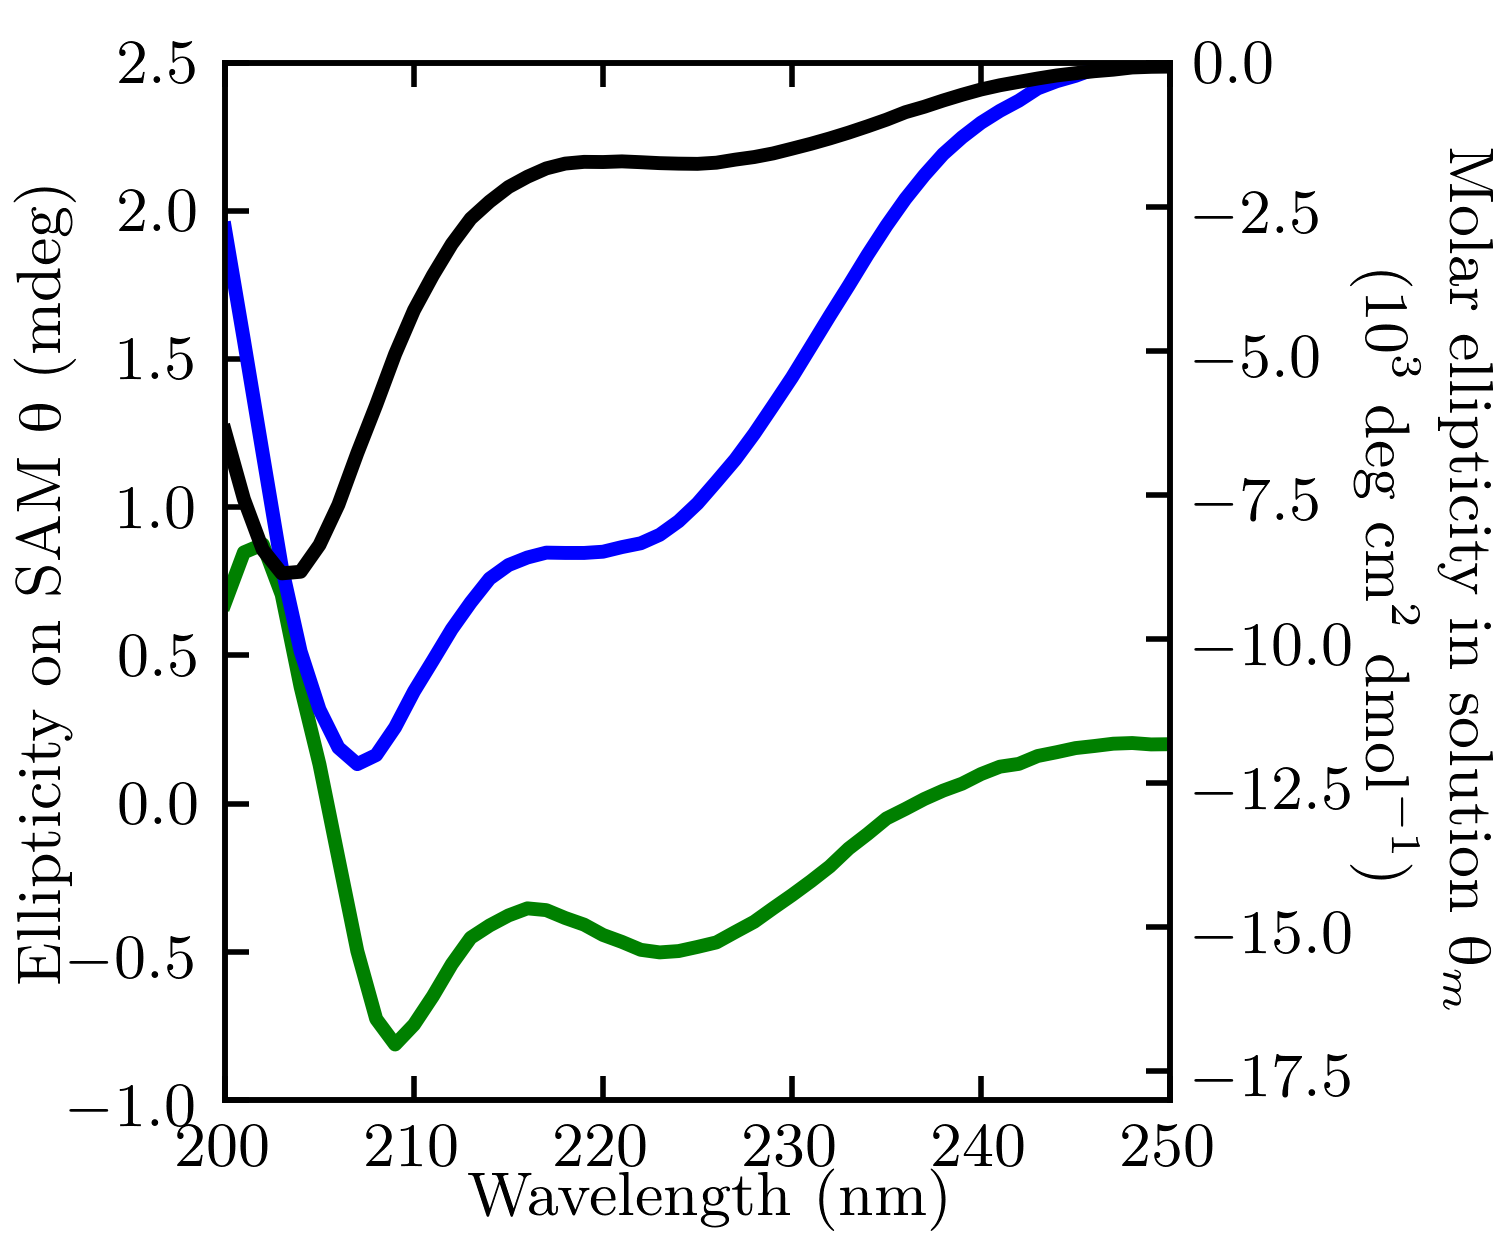
\includegraphics[width=3.25in]{figures-helix/nachos_cd_spectra.png}
    \caption{
        Circular dichroism spectra of \pep{} in three different solvent environments. 
        Black: \pep{} dissolved in aqueous Tris buffer. 
        Blue: \pep{} dissolved in \tbawat{}. 
        Green: \pep{} covalently attached to a SAM of decanethiols on Au. 
        The left vertical axis is the ellipticity for the peptide on the surface, and the right vertical axis is the ellipticity of the peptide in the two solutions. 
        Adapted from ref \citenum{Gallardo2012}.
    }
    \label{fig:helix-cd_spectra}
\end{figure}

Simulating the structural change demonstrated between these two solvents and the surface environment has proven to be a challenge. 
For example, Di Pierro et al. showed that simply by moving from water to the binary solvent, \tbawat{}, the OPLS force field failed to describe the experimental data \cite{DiPierro2015}.   
The authors reoptimized the \tba{} parameters to interact properly with \ce{H2O} by using a refinement algorithm that systematically minimized the difference between experimental Kirkwood-Buff integrals and the radial distribution functions between \tba{} and water \cite{DiPierro2015}. 
Adding the complexity of an inorganic surface to a simulation is an additional challenge \cite{Walsh2017}. 
Although there are several recent successful simulations of a bio/abio interface, these are less common for several reasons \cite{Gianese2009, Meibner2014, Zerze2015, Cannon2015, Krause2017, Prakash2018a, Prakash2018, Sprenger2018}.
Surface simulations require robust experimental data on the structure of the surface in order to construct an atomically accurate model. 
Further, force field parameters of the surface moieties are rare and often not intended to work with biomolecular force fields \cite{Latour2008, Latour2014}.
Polarization effects of metallic surfaces, such as image charges \cite{Heinz2011}, require additional considerations \cite{Iori2009}. 
However, the biomimetic surface strategy implemented in our published work directly addresses many of these challenges. 
Robust structural data of SAMs is available from surface-averaged spectroscopies such as Fourier transform infrared (FTIR), spatially-resolved scanning tunneling microscopy, and theoretical studies; 
parameters for saturated hydrocarbons are readily accessible and can be combined with biomolecular force fields; 
and the SAM mitigates the electrostatic effects of image charges in gold.

Here, we present MD simulations of \pep{} that successfully capture the experimentally measured solvent- and surface-induced conformational change in water, \tbawat{}, and on the surface of a decanethiol SAM. 
Structural assignments were performed with the Define Secondary Structure of Proteins (DSSP) algorithm and show that the simulations quantitatively captured the amount of secondary structure of \pep{} in each of the three environments when compared to deconvolutions of the experimental CD spectra. 
Theoretical CD spectra were calculated from the MD trajectories using DichroCalc and were in qualitative agreement with experiment. 
These simulations demonstrated that the OPLS-AA force field was sufficiently accurate in \tbawat{} and on the surface of a SAM, despite being parameterized for biomolecules in aqueous solution. 
Herein we describe our simulation setup and protocol, followed by an extensive discussion of the results of the simulations and comparison to the experimental spectra\cite{Gallardo2012} reproduced in Figure \ref{fig:helix-cd_spectra}. 
After demonstrating the validity of our simulations, we present an additional set of simulations designed to explore the mechanism of folding of the peptide on the SAM surface and propose two hypotheses that are currently being experimentally tested in our laboratory.

%%%%%%%%%%%%%%%%%%%%%%%%%%%%%%%%%%%%%%%%%%%%%%%%%%%%%%%%%%%%%%%%
%%%%%%%%%%%%%%%%%%%%%%%%%%%%%%%%%%%%%%%%%%%%%%%%%%%%%%%%%%%%%%%%
\section{Methods}\label{helix-methods}
%%%%%%%%%%%%%%%%%%%%%%%%%%%%%%%%%%%%%%%%%%%%%%%%%%%%%%%%%%%%%%%%
%%%%%%%%%%%%%%%%%%%%%%%%%%%%%%%%%%%%%%%%%%%%%%%%%%%%%%%%%%%%%%%%

\subsection{System preparation and force field parameters}

A template of \pep{} was created in a \textalpha{}-helical conformation using the Avogadro molecular editing package\cite{Hanwell2012}.
The propargylglycines, which provided the alkyne group for the ``click'' reaction in the experiment, were replaced with glycine residues. 
Because of the short length of the peptide, the N and C termini were neutralized with an amide group and acetyl group, respectively. 
Parameters for the united atom model of \tba{} (Figure \ref{fig:helix-tba}) were adapted for Gromacs from Di Pierro et al \cite{DiPierro2015}.
To validate our implementation of the \tba{} parameters, we calculated the solvent pair correlation functions of a 0.2 mol fraction \tba{} in \ce{H2O} mixture and found that our calculated pair correlation functions matched those reported in Di Pierro et al. (Figure \ref{fig:helix-rdfs}, compare to Figure 6 of ref \citenum{DiPierro2015}). 
Generally, it is best to avoid combining all-atom models with united-atom models; 
however, in this case, the \tba{} parameters were reoptimized explicitly for mixtures with the TIP3P water model. 
While parameters for decanethiols in SAMs have been published and validated before\cite{Godawat2009}, we wanted to use a consistent force field in all three environments. 
Because of this, parameters for decanethiol within the SAM were adapted from existing OPLS-AA parameters for hydrocarbons\cite{Kaminski1994}. 
Using restricted Hartree-Fock calculations in the GAMESS QM software package\cite{Schmidt1993, Gordon2005}, partial charges were attained by minimizing a decanethiol molecule using the 6-31G basis set and fitting charges to the electrostatic potential calculated at the Connolly surface using the 6-31G(d) basis set. 
Derived charges are shown in Figure \ref{fig:helix-charges}. 
All subsequent calculations used the Gromacs 2016.3 molecular dynamics simulation package\cite{Berendsen1995, Lindahl2001, VanDerSpoel2005, Hess2008, Pronk2013, Pall2015, Abraham2015} and the OPLS-AA force field\cite{Jorgensen1996, Kaminski2001} unless otherwise noted.

\begin{figure}
    \center
    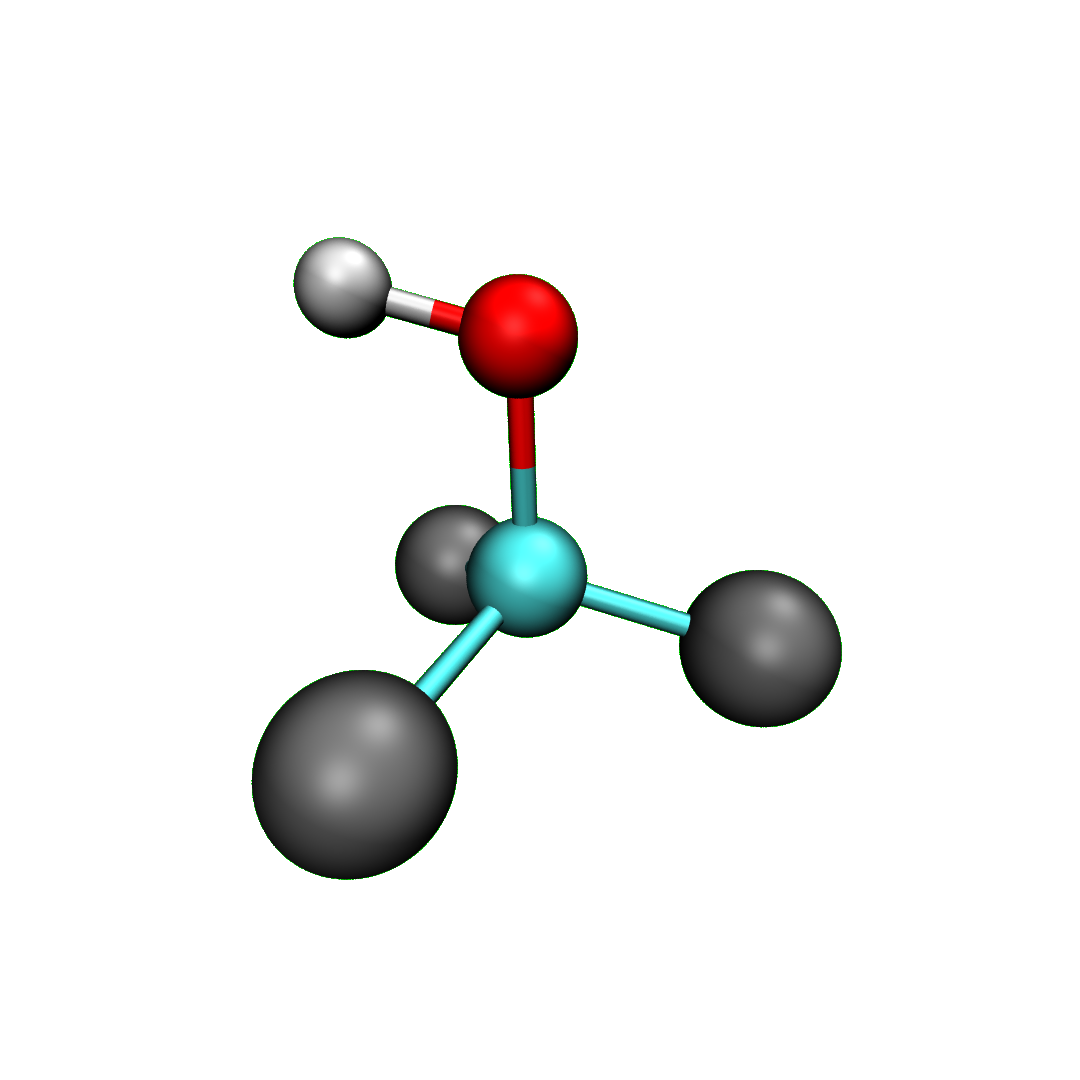
\includegraphics[width=3.25in]{figures-helix/tba.png}
    \caption{
        A united atom model of \emph{tert}-butanol used in these simulations. 
        The white sphere represents a hydrogen, the red sphere represents an oxygen, the cyan sphere represents the central carbon, and the gray spheres represent united-atom representations of the three methyl groups.
    }
    \label{fig:helix-tba}
\end{figure}

\begin{figure}
    \center
    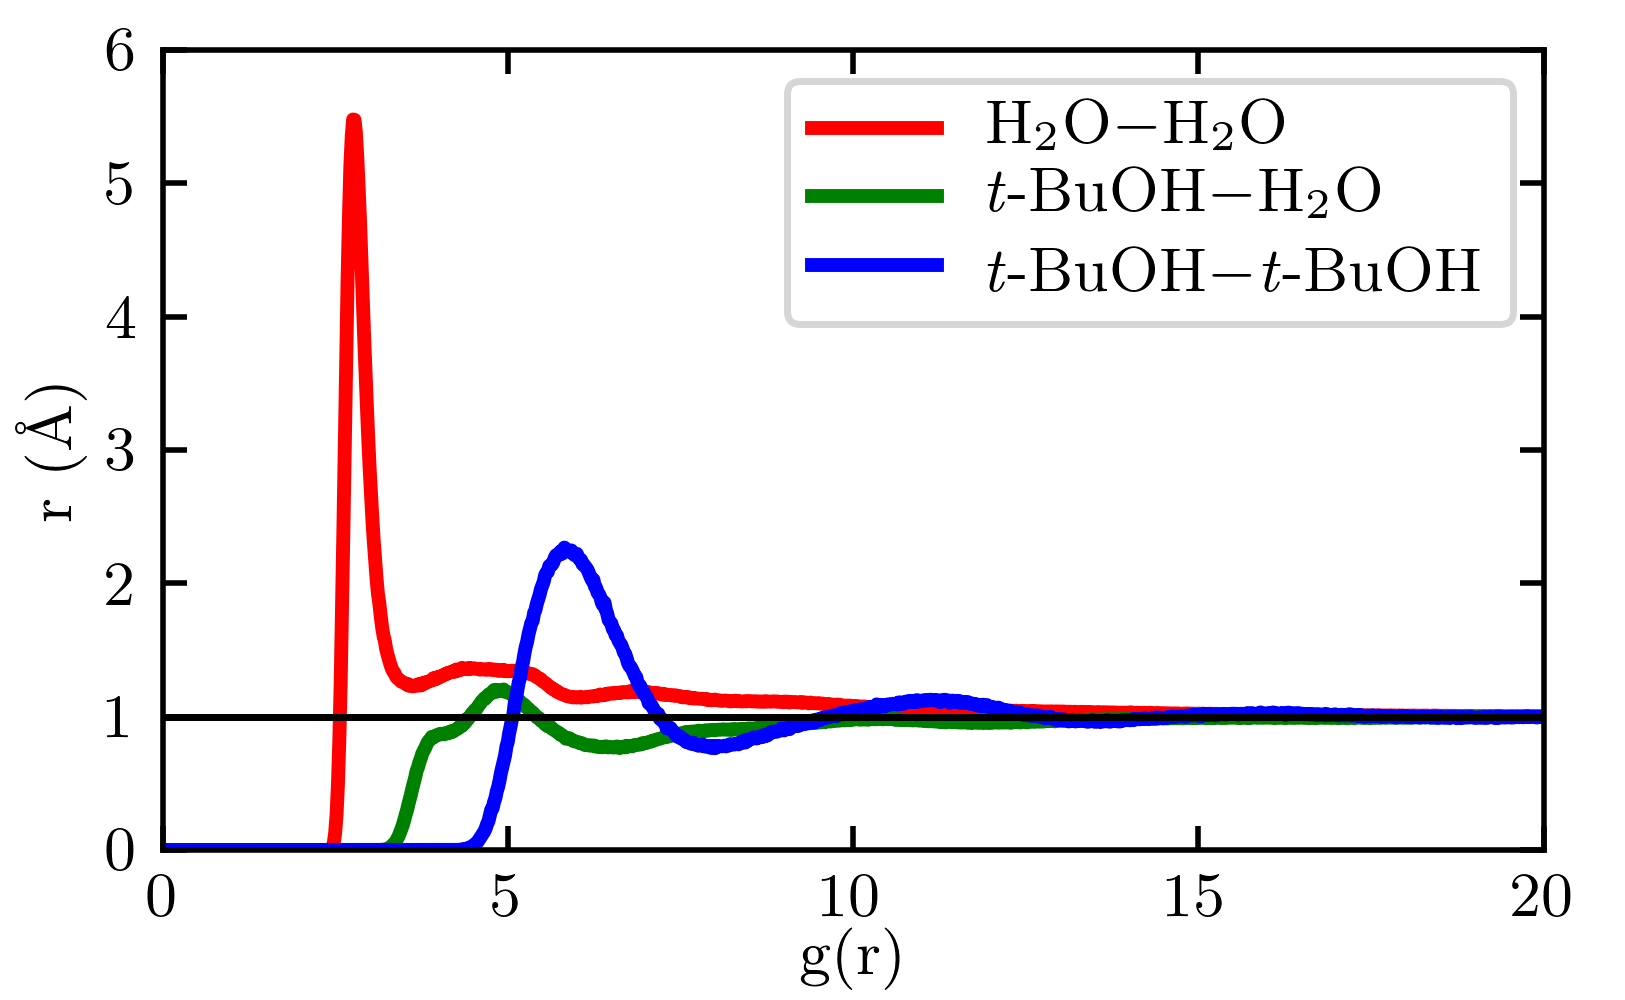
\includegraphics[width=3.25in]{figures-helix/rdfs.png}
    \caption{
        Pair correlation functions matched those reported in ref \citenum{DiPierro2015} indicating that the \tba{} parameters were implemented correctly for Gromacs. 
        Red: Pair correlation function between the oxygen atoms of water molecules and the oxygen atoms of other water molecules. 
        Green: Pair correlation function between the central carbon of \tba{} and the oxygen atoms of water molecules. 
        Blue: Pair correlation function between the central carbon atom of \tba{} and the central carbon atoms of other \tba{} molecules. 
    }
    \label{fig:helix-rdfs}
\end{figure}

\begin{figure}
    \center
    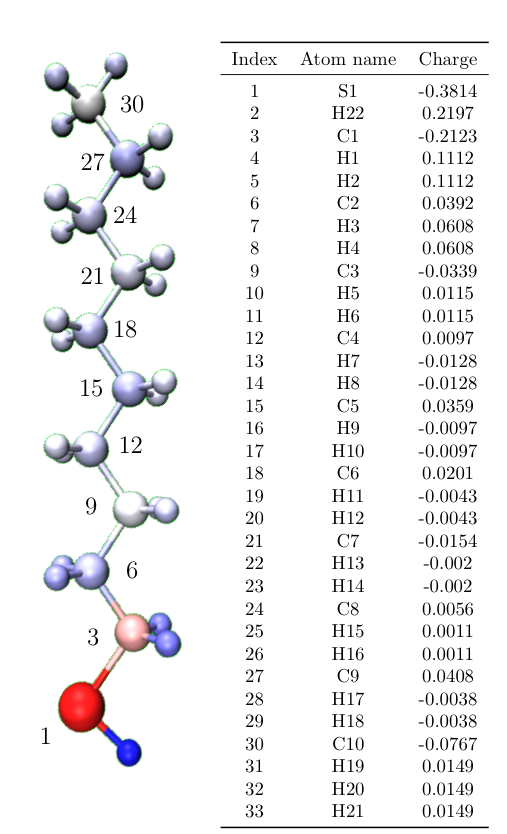
\includegraphics[width=3.25in]{figures-helix/charge_figure.png}
    \caption{
        Derived partial charges for the decanethiol molecule used in the SAM. 
        The atoms are colored by charge, where red represents a more negatively charged atom, and blue represents a more positively charged atom. 
        The heavy atoms are indexed and the partial charges can be found in the table. 
        Hydrogens appear under the heavy atom to which they are bound.
    }
    \label{fig:helix-charges}
\end{figure}

\subsection{Water simulation}

The peptide was minimized in vacuum using the steepest descent algorithm and solvated in a 7.6 nm cubic box of TIP3P water \cite{Jorgensen1983}. 
The solvated system was then minimized using the steepest decent algorithm, heated to 300 K under the NVT ensemble for 50 ps, and equilibrated under the NPT ensemble at 1 atm for 100 ps, each with heavy atom restraints on the peptide atoms. 
This equilibrated system was used to begin the simulation of the folded peptide in water. 

\subsection{Binary mixture simulation}

A 2:1 (v/v) \tba{}:\ce{H2O} mixture was created by distributing 1831 molecules of united atom \tba{} (Figure \ref{fig:helix-tba}) and 4862 TIP3P water molecules in a 7.6 nm cubic box. 
This box was energy minimized using the steepest descent algorithm, heated to 300 K under the NVT ensemble for 50 ps, and equilibrated under the NPT ensemble at 1 atm for 100 ps. 
The starting peptide was then energy minimized using the steepest descent algorithm and placed inside the equilibrated solvent mixture. 
The system was again energy minimized using the steepest descent algorithm, then heated to 300 K under the NVT ensemble for 50 ps, and equilibrated under the NPT ensemble at 1 atm for 100 ps. 
This equilibrated system was used to begin the simulation of the folded peptide in \tbawat{}. 

\subsection{SAM surface simulation}

A SAM was built by placing decanethiol molecules in a hexagonal packing arrangement according to Ulman et al.\cite{Ulman1989}, with an intermolecular spacing of 4.97 \si{\angstrom}, using an in-house Python code and the gmx insert-molecules module. 
To simulate bonds from the decanethiols to the Au surface, which was not present in the simulations, the sulfur atoms of the decanethiols were restrained to their horizontal $x$-$y$ plane with a harmonic restraint of $2\cdot10^3$ kJ mol$^{-1}$ nm$^{-2}$. 
The SAM was energy minimized using the steepest descent algorithm, and then heated to 300 K under the NVT ensemble for 50 ps. 
Separately, the starting peptide was energy minimized using the steepest descent algorithm and solvated in a 6.0 nm $\times$ 7.0 nm $\times$ 6.0 nm box of TIP3P water. 
The $x$, $y$ dimensions were matched to the dimensions of the decanethiol layer. 
The $z$ dimension was chosen to ensure that the peptide cannot interact with the bottom of the decanethiol layer across the periodic boundary. 
The solvated system was then energy minimized using the steepest decent algorithm, headed to 300 K under the NVT ensemble for 50 ps, and equilibrated under a semi-isotropic NPT ensemble at 1 atm for 100 ps with volumetric fluctuations restricted to the $z$ dimension, each with heavy atom restraints on the peptide atoms. 

The solvated system and the SAM were then combined so that the peptide was 6.822 \si{\angstrom} away from the top of the SAM. 
Again, in order to mitigate the effect of the sulfur layer of the SAM across the $z$-dimension of the periodic boundary conditions, the size of the water layer in between the peptide and the neighboring sulfur layer was chosen to be much larger than the electrostatic cutoff of the simulations. 
An illustration of this system is shown in Figure \ref{fig:helix-system}. 
The azido linker group, which covalently bonds the peptide to the SAM surface in experiment, was approximated with a harmonic restraint of 103 kJ mol$^{-1}$ nm$^{-2}$ and equilibrium bond length of 6.822 \si{\angstrom} between the Gly C\textalpha{} atoms and the C10 of the nearest decanethiol molecule. 
This distance, which is illustrated in Figure \ref{fig:helix-linker}, was chosen based on a DFT energy minimized structure at the wB97X-D/6-311$+$G** level using the Spartan QM software suite\cite{Shao2006}.   
The system was again energy minimized using the steepest descent algorithm, heated to 300 K under the NVT ensemble for 50 ps, then equilibrated under the NPT ensemble at 1 atm for 100 ps with volumetric fluctuations restricted to the $z$ dimension. 
The harmonic restraints binding the peptide to the SAM were removed for the production simulation, unless otherwise noted.

\begin{figure}
    \center
    \includegraphics[width=3.25in]{figures-helix/system3.png}
    \caption{A snapshot of the starting configuration for \pep{} on the surface of a decanethiol SAM. The peptide (cyan ribbon) is shown in the folded starting configuration, with lysine residues (red) facing up away from the SAM and leucine residues (gray) facing down toward the SAM. The yellow, cyan, and white spheres are the sulfur, carbon, and hydrogen atoms, respectively, of the decanethiol molecules. The small red and white sticks represent water molecules. The green spheres in solution represent chloride ions. }
    \label{fig:helix-system}
\end{figure}

\begin{figure}
    \center
    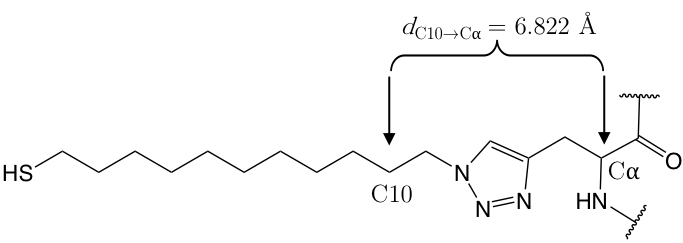
\includegraphics[width=6.00in]{figures-helix/Linker_figure.png}
    \caption{
        The product of the Huisgen cycloaddition. 
        The long alkane chain sits in a SAM of decanethiols, and the sulfur atom is covalently attached to a Au(111) surface. 
        The C\textalpha{} is from one of the two propargylglycine residues of \pep{}. 
        For simplicity, we have replaced the propargylglycine with a glycine residue in the simulations. 
        The C\textalpha{} of the glycine residues were harmonically restrained to the nearest C10 on the SAM at a distance of 6.822 \si{\angstrom} (the distance in the DFT geometry optimized structure) during the annealing process and were kept or removed for the production simulations, as discussed in the main text.
    }
    \label{fig:helix-linker}
\end{figure}

\subsection{Simulated Annealing}\label{helix-anneal}

In order to prepare the unfolded structure in each of the solvent environments, the heavy atom restraints on the protein were removed. 
Using the Berendsen thermostat, the systems were coupled to a heat bath that increased by 12 K every 10 ps for 500 ps. 
The systems were equilibrated at 900 K for 100 ps, and then coupled to a heat bath that decreased by 12 K every 10 ps for 500 ps. 
A representative temperature curve from this annealing process is shown in Figure \ref{fig:helix-anneal}A. 
For the simulations that included a SAM layer, harmonic restraints of 107 kJ mol$^{-1}$ nm$^{-2}$ were applied during the annealing process to the heavy atoms of the SAM to keep the layer intact. 
Each system was visually inspected to confirm the peptide had unfolded during the annealing process. 
The DSSP structural assignments (see below) showed complete unfolding for each peptide; 
these are shown in Figures \ref{fig:helix-anneal}, \ref{fig:helix-anneal}C, and \ref{fig:helix-anneal}D for the peptide in water, \tbawat{}, and on the SAM surface respectively.

\begin{figure}
    \center
    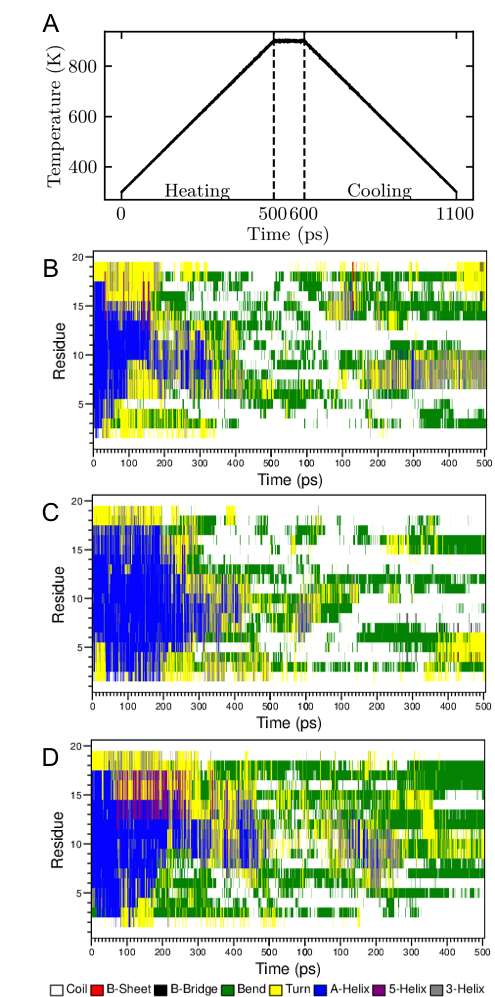
\includegraphics[width=2.75in]{figures-helix/unfolding.png}
    \caption{
        A: Temperature curve for the simulated annealing process used to generate the unfolded structures. 
        The dashed lines separate the stages of the annealing process. 
        B, C, and D: DSSP structural assignments for \pep{} in water, in \tbawat{} and on the SAM, respectively, during the annealing process. 
        Note that all of the initial structure is lost in each system in the first 500 ps (the heating stage). 
        The final structure from the annealing process was used to initiate the simulations of the unfolded peptide in each solvent environment.
    }
    \label{fig:helix-anneal}
\end{figure}

\subsection{Production simulations and analyses}

For each of the three environments, a production simulation was run from a folded structure of the peptide and from an unfolded structure of the peptide, resulting in six simulations. 
Simulations were run for 1.25 \textmu{}s each, using a 2 fs time step and a stochastic integrator. Particle-mesh-Ewald (PME) electrostatics was implemented with a Coulombic cutoff of 10 \si{\angstrom}. 
Van der Waals (VDW) interactions were cut off at 10 \si{\angstrom}. 
Snapshots were recorded every 4 ps during simulations.

Structural assignments were calculated using the DSSP algorithm (discussed further below)\cite{Kabsch1983, Joosten2011} through the gmx do\_dssp interface. 
Radii of gyration ($R_g$), RMSDs, pair correlation functions, and free energy surfaces were calculated using gmx modules. 
Cluster analyses were performed using the Gromos algorithm\cite{Daura1999} and the gmx cluster module with a cutoff of 2.5 \si{\angstrom} backbone RMSD between clusters. 
CD line spectra were computed at every 100 ps using the DichroCalc portal\cite{Bulheller2009, Jasim2018} using both the Hirst basis set\cite{Hirst1998, Besley1999} and the Woody basis set\cite{Woody1999}, both with backbone transfer transitions. 
All other options were left as default. 
The line spectra were then convoluted with Gaussian functions to produce continuous spectra, as discussed in the main text.

%%%%%%%%%%%%%%%%%%%%%%%%%%%%%%%%%%%%%%%%%%%%%%%%%%%%%%%%%%%%%%%%
%%%%%%%%%%%%%%%%%%%%%%%%%%%%%%%%%%%%%%%%%%%%%%%%%%%%%%%%%%%%%%%%
\section{Results}\index{helix-results}
%%%%%%%%%%%%%%%%%%%%%%%%%%%%%%%%%%%%%%%%%%%%%%%%%%%%%%%%%%%%%%%%
%%%%%%%%%%%%%%%%%%%%%%%%%%%%%%%%%%%%%%%%%%%%%%%%%%%%%%%%%%%%%%%%

In order to successfully and reliably integrate proteins onto inorganic materials, it is necessary to attach them reproducibly to surfaces and substrates with the appropriate structure, orientation, and chemical environment for function. 
Understanding any conformational changes that are imparted by the surface material is critical to this goal but is a longstanding challenge \cite{Hlady1996, Castner2002, Latour2005biomaterials}.
In order to test if the generally applicable force field (OPLS-AA) is reliable at a surface for the \pep{} peptide and can capture conformational changes that are potentially critical to its ability to noncovalently immobilize proteins at a surface in a biomimetic fashion, we used MD simulations to investigate the known solvent-induced and surface-induced structural changes of the peptide.

\subsection{Conformational differences and sampling}

Previously, CD spectra (Figure \ref{fig:helix-cd_spectra}) had indicated that \pep{} was unfolded in aqueous solution, partially helical in \tbawat{}, and significantly helical on the surface of a decanethiol SAM \cite{Gallardo2012}. 
To avoid biasing the simulations by starting structure, we ran two separate trajectories for each of the three solvent environments: one from a folded \textalpha{}-helix and one from an unfolded, disordered structure. 
We then ran MD simulations on each of the six systems for 1.25 \textmu{}s. 
At each frame of the trajectories we then calculated the peptide secondary structure using the DSSP algorithm\cite{Kabsch1983, Joosten2011}, which categorizes residues into eight classifications based on estimated hydrogen bonding energies: \textalpha{}-helix, $3_{10}$-helix, \textpi{}-helix, turn, \textbeta{}-sheet, \textbeta{}-bridge, bend, and coil. 
The total breakdown of secondary structure by residue is plotted against simulation time for each of the six trajectories in Figure \ref{fig:helix-dssp}. 
Since we are interested in a more broadly defined structural change, we grouped each of these secondary structures into four larger categories: 1) helical (\textalpha{}-helix, $3_{10}$-helix, or \textpi{}-helix); 2) turn; 3) strand (\textbeta{}-sheet, \textbeta{}-bridge, or bend); and 4) unfolded (coil). 
The fraction of residues in each of these categories was calculated, binned to smooth the data, and plotted in Figure \ref{fig:helix-conf_fracs}, where dark blue represents the fraction of residues in a helical conformation, light blue represents the fraction of residues in a turn, green represents the fraction of residues in a strand, and red represents the fraction of residues in an unfolded conformation. 
Each category is offset on the $y$-axis to avoid overlap and will be referred to hereafter as the stacked ``conformational fractions.'' 

\begin{figure}
    \center
    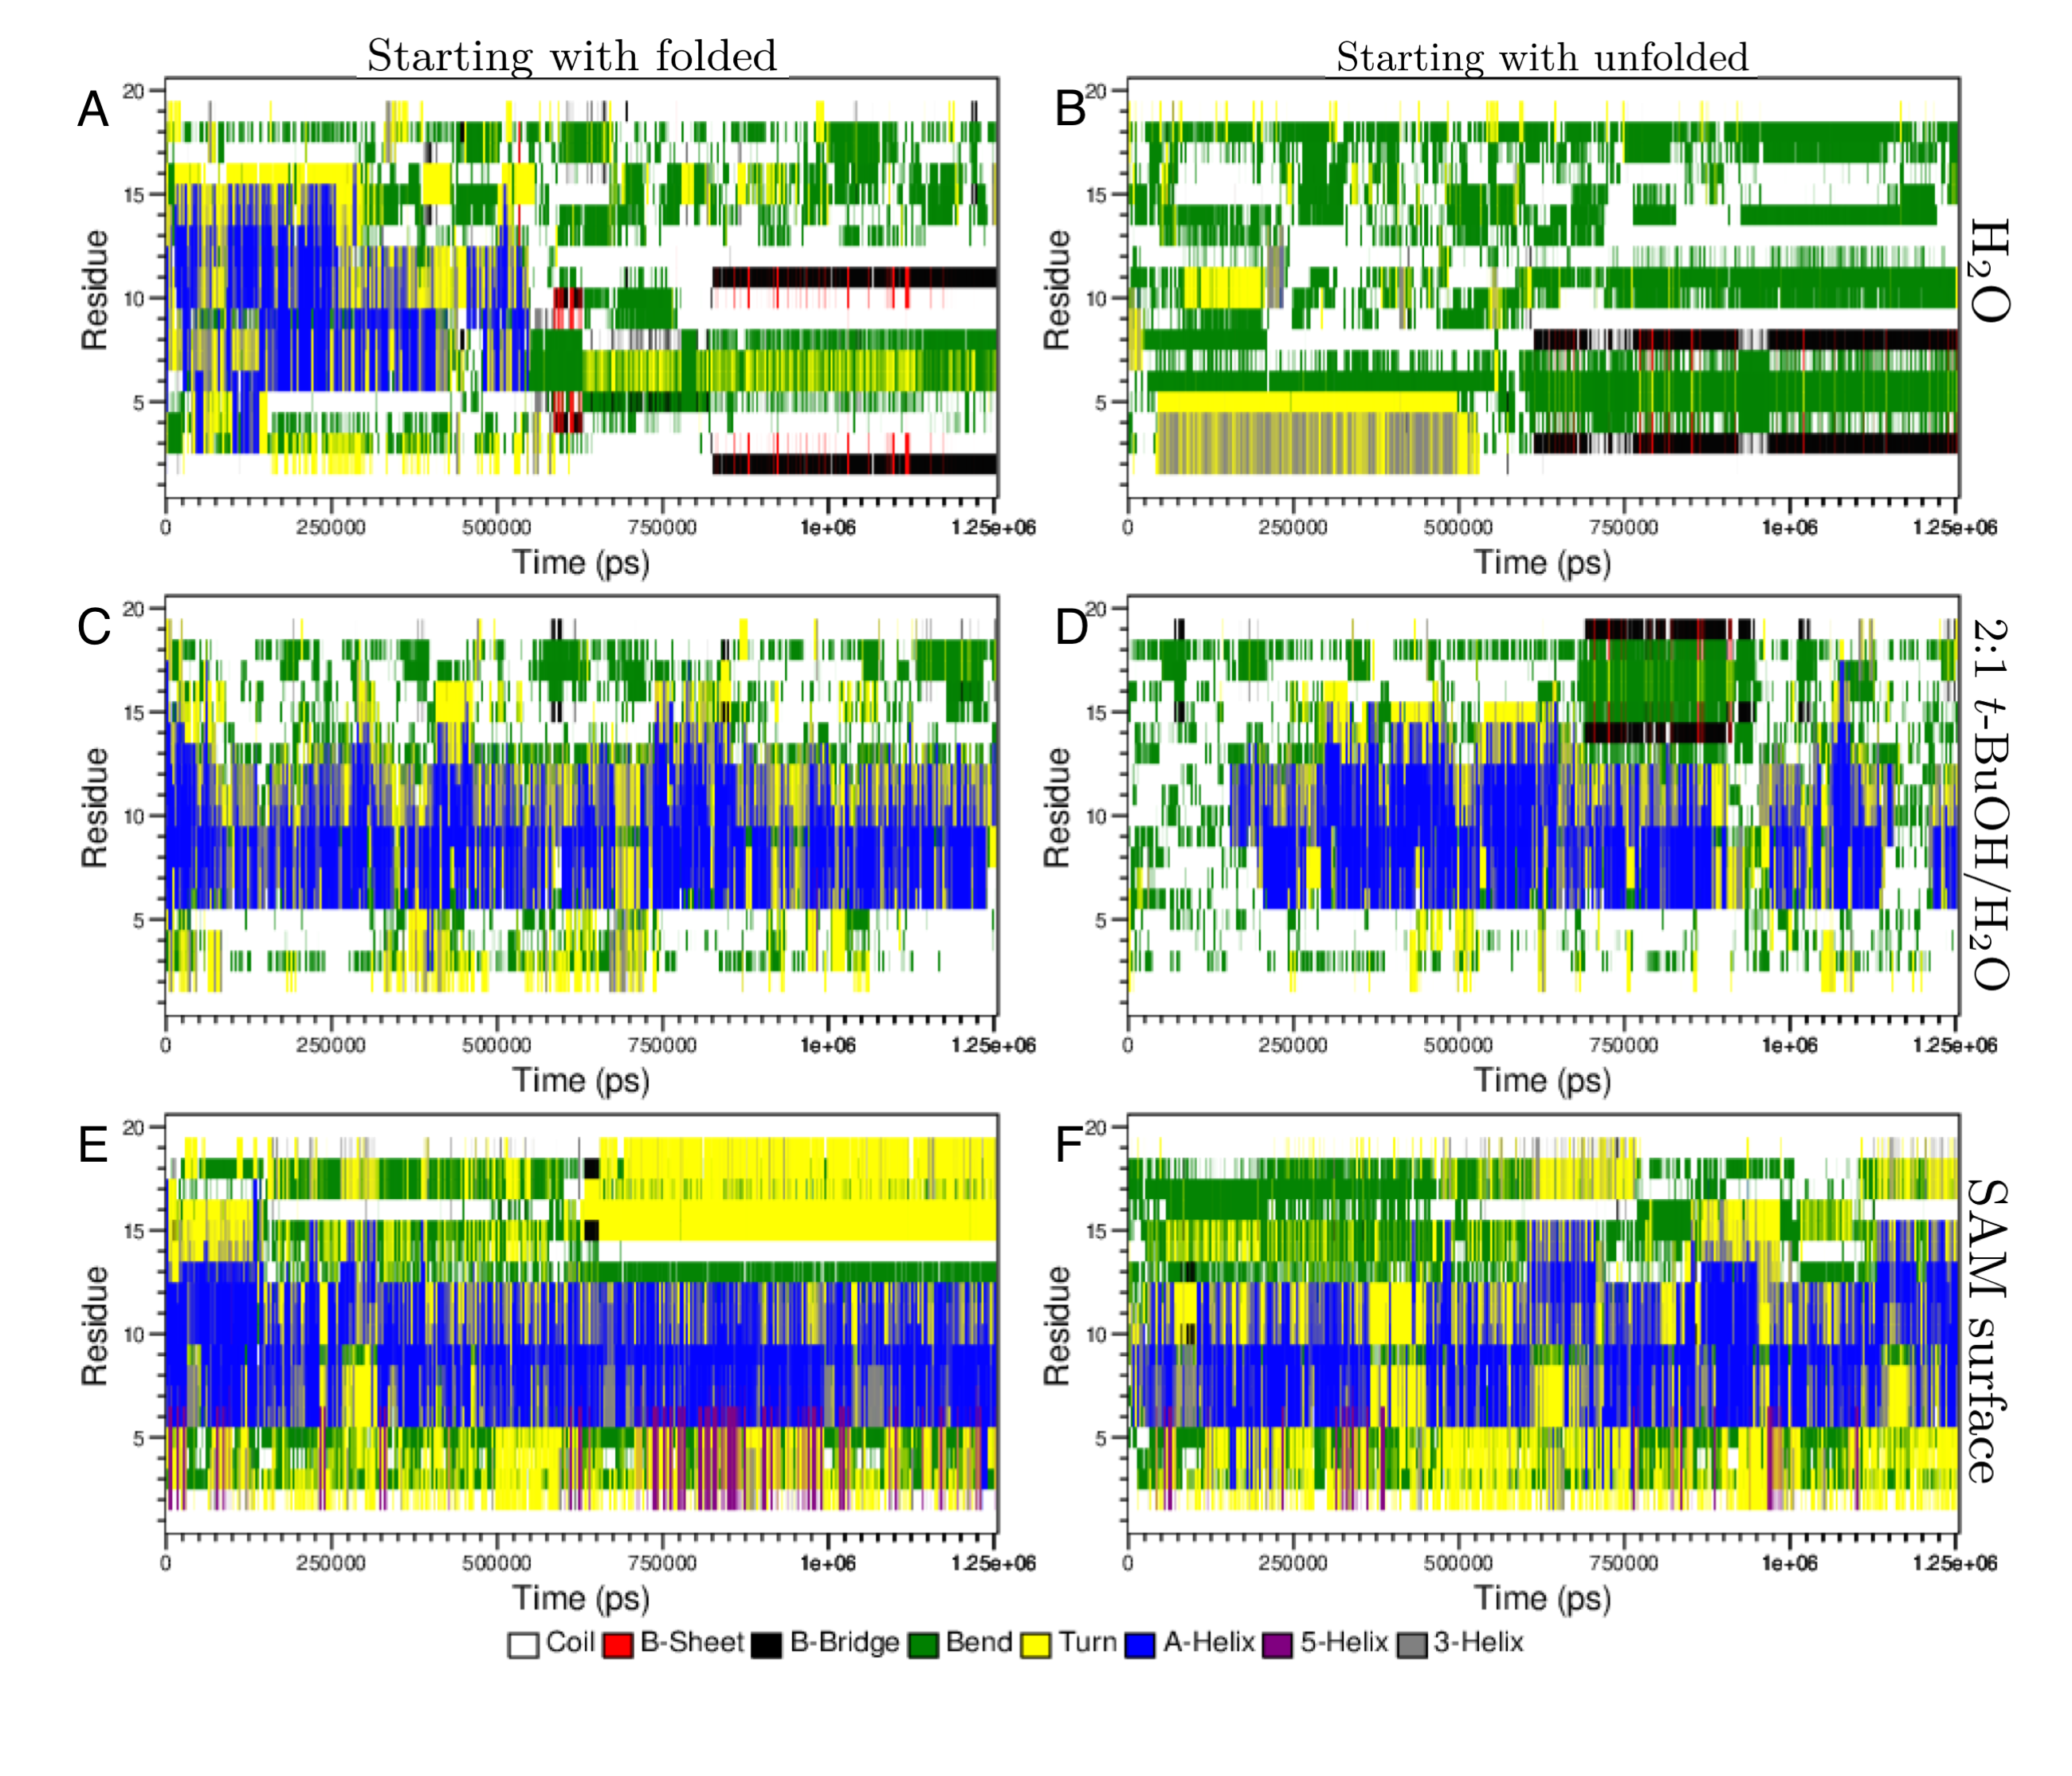
\includegraphics[width=6.0in]{figures-helix/dssp.png}
    \caption{
        DSSP structural assignments by residue for simulations of \pep{}. 
        A, C, E: \pep{} began the simulation in an \textalpha{}-helical conformation. 
        B, D, F: \pep{} began the simulation unfolded.
        A, B: the peptide was dissolved in water. 
        C, D: the peptide was dissolved in \tbawat{}. 
        E, F: the peptide was on the surface of a SAM dissolved in water.
    }
    \label{fig:helix-dssp}
\end{figure}

\begin{figure}
    \center
    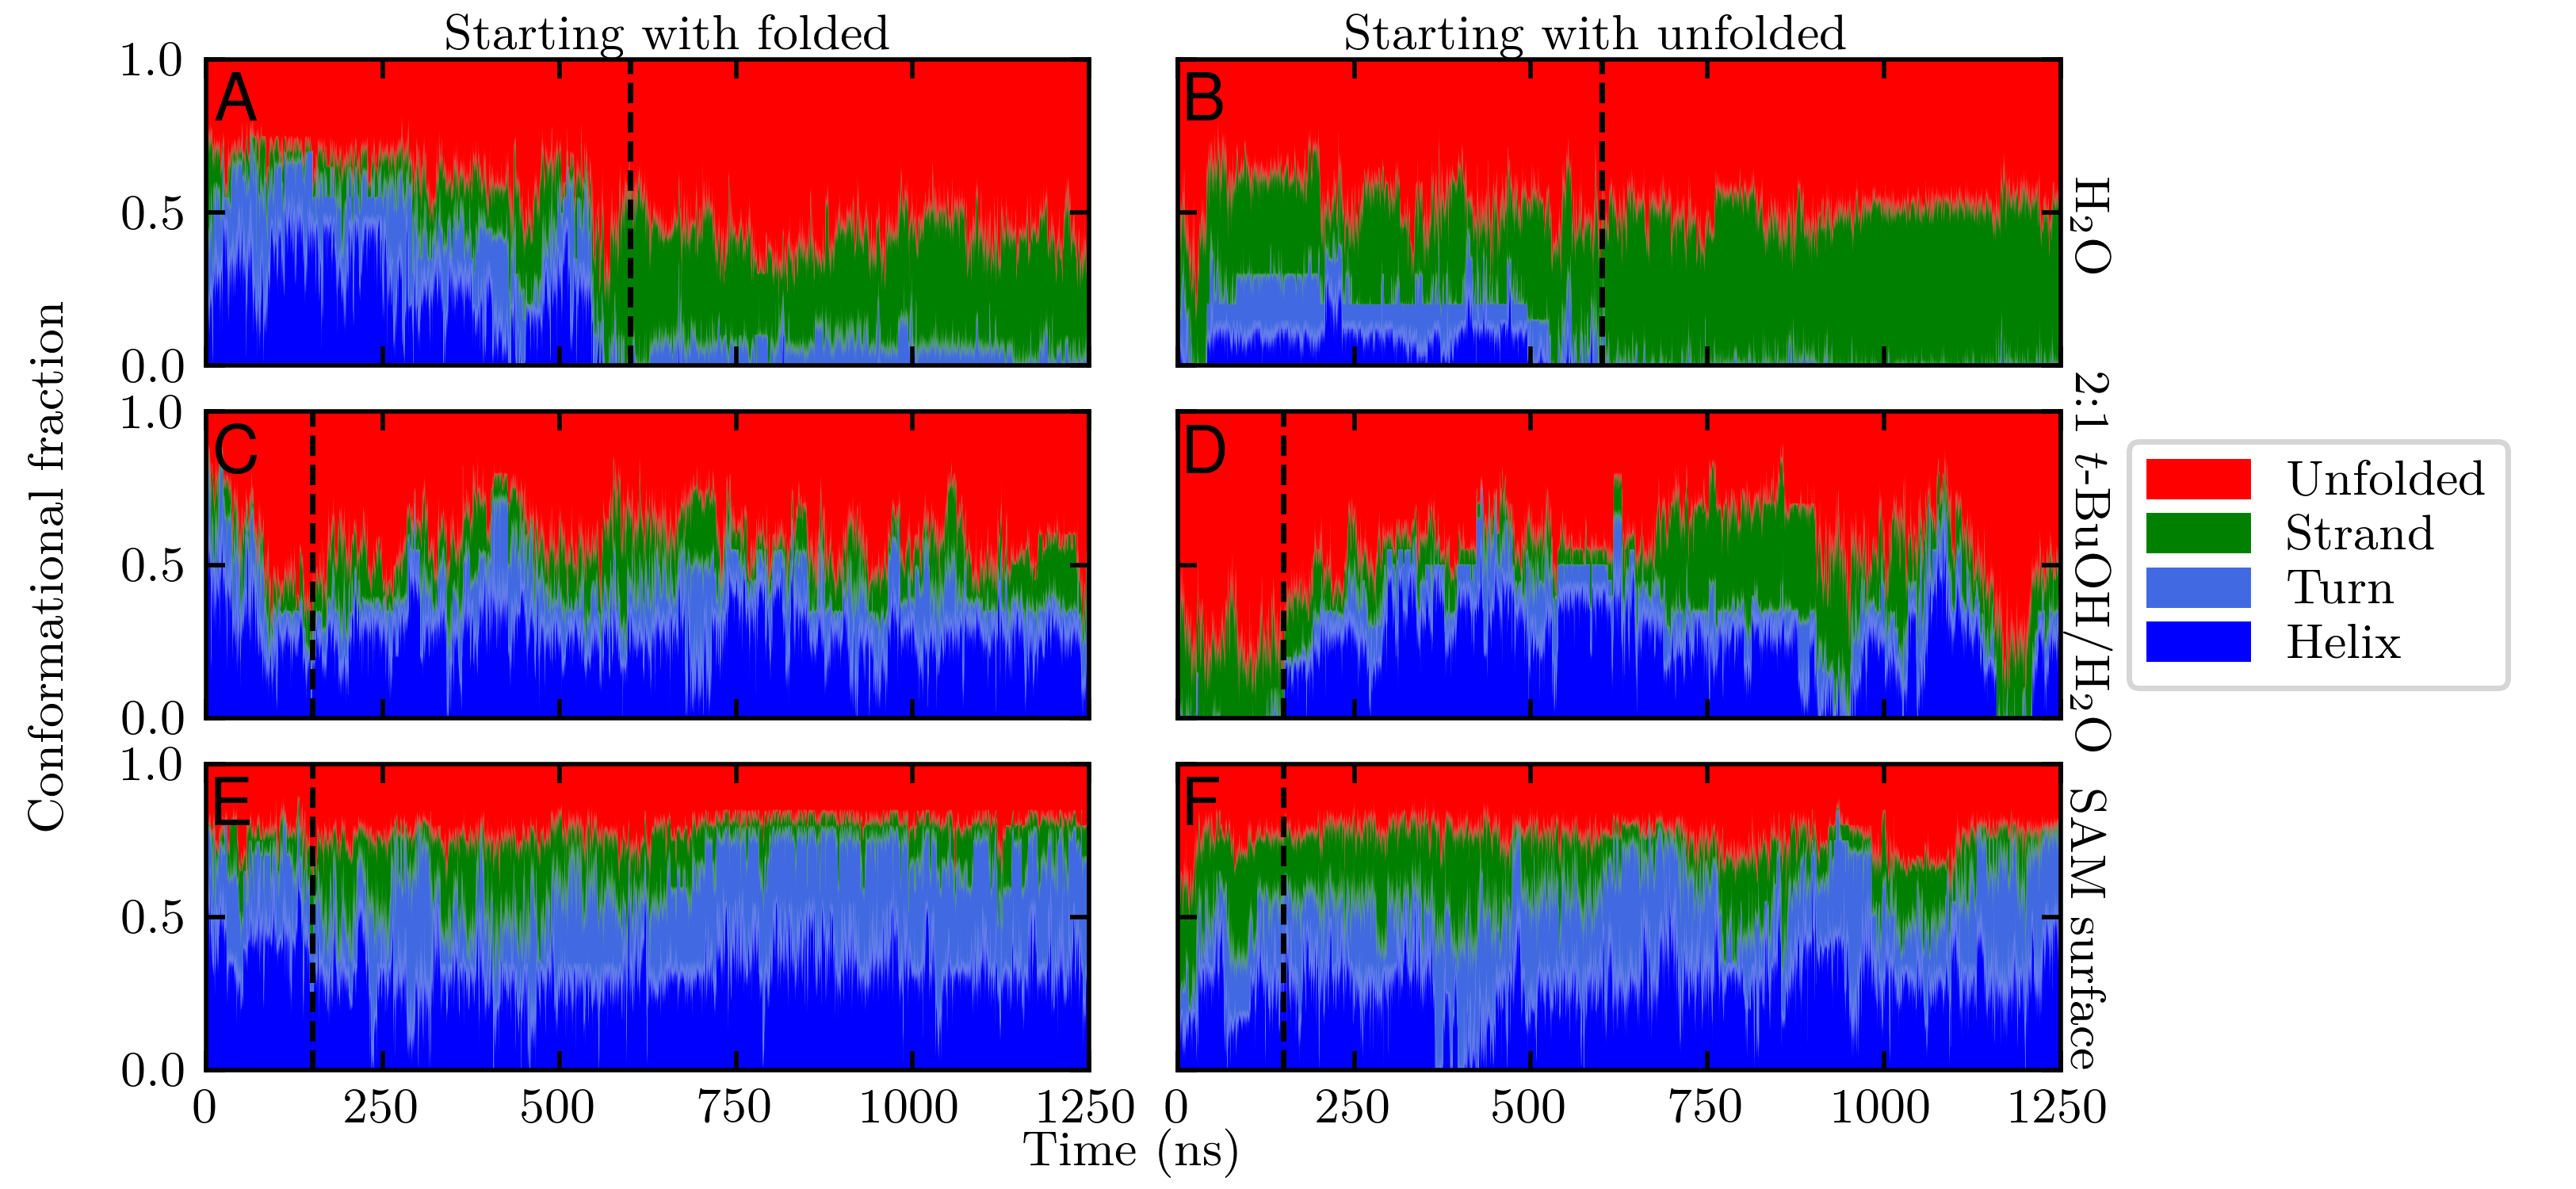
\includegraphics[width=6.0in]{figures-helix/combined_helicity.png}
    \caption{
        Stacked conformational fractions of \pep{} in three different solvent environments. 
        Blue: fraction of residues assigned to a helical secondary structure. 
        Light blue: fraction of residues assigned to a turn secondary structure. 
        Green: fraction of residues assigned to a strand secondary structure. 
        Red: fraction of residues assigned to unfolded secondary structure (see main text). 
        A, C, E: \pep{} began the simulation in a \textalpha{}-helical conformation. 
        B, D, F: \pep{} began the simulation unfolded. 
        A, B: the peptide was dissolved in water. 
        C, D: the peptide was dissolved in \tbawat{}. 
        E, F: the peptide was on the surface of a SAM dissolved in water. 
        The black dashed lines represent the determined equilibration time for each simulation. 
        The data after this mark was averaged and is presented in Table \ref{tbl:helix-frac_bestsel}.
    }
    \label{fig:helix-conf_fracs}
\end{figure}

When the simulation of \pep{} in water was initiated from a folded helical conformation (Figure \ref{fig:helix-conf_fracs}A), the peptide began the simulation with high helical character (0.70 helical and 0.15 turn). 
For the first 600 ns, the helical character of the peptide slowly decreased, resulting in an unfolded peptide. 
After this time, the peptide adopted significant strand character (average of 0.36 strand), which was retained through the duration of the simulations. 
Figure \ref{fig:helix-dssp}A shows that the strand character mostly occurred at the N-terminal region (residues 2-11), and the rest of the peptide was unstructured. 
Starting from an unfolded conformation in water (Figure \ref{fig:helix-conf_fracs}B), the peptide began with little helical or turn character. 
For the first 600 ns, the peptide sampled conformations with some helical character and some strand character, but eventually adopted a conformation with no helical character and high strand character (average of 0.50 strand). 
Figure \ref{fig:helix-dssp}B shows that the strand character occurred again at the N-terminal region (residues 3-8), and the rest of the peptide was unstructured. 
Despite starting from very different conformations, both simulations of \pep{} in water displayed similar secondary structure, with strand character at the N-terminal region and the rest of the peptide unstructured. 
Because 600 ns elapsed before \pep{} adopted similar secondary structure in both simulations, 600 ns was taken to be the equilibration time for both of these simulations, and the first 600 ns of these trajectories was not included in the analyses that follow for \pep{} in water.

When the simulation of \pep{} in \tbawat{} was started from a folded helical conformation (Figure \ref{fig:helix-dssp}C), the peptide began the simulation with significant helical character (0.80 helical and 0.10 turn). 
Over the first 150 ns, the helical fraction decreased rapidly to ~0.3 and the unfolded character increased to ~0.5. 
This helicity was then retained for the duration of the simulation. 
Figure \ref{fig:helix-dssp}C shows that the helicity was lost at residues 1-5 and 15-20 (the two terminal regions), and the middle region of the peptide (residues 6-14) remained helical. 
Starting from an unfolded conformation in \tbawat{} (Figure \ref{fig:helix-conf_fracs}D), the peptide began the simulation with little helical character. 
For the first 150 ns, the peptide sampled configurations with mostly unfolded character, and after this time the peptide primarily sampled helical configurations that were retained through the duration of the simulation. 
Figure \ref{fig:helix-dssp}D shows that the helical character was again in the middle region of the peptide (residues 6-14), and the unfolded character dominated the two terminal regions (residues 1-5 and 15-20). 
Again, despite starting from very different conformations, both simulations of \pep{} in \tbawat{} displayed similar secondary structure. 
Because 150 ns elapsed before the peptide attained this secondary structure, 150 ns was taken to be the equilibration time for both of these simulations, and the first 150 ns of these trajectories was not included in the analyses that follow for \pep{} in \tbawat{}. 

Finally, when the simulation of \pep{} on the surface of a SAM was started from a folded helical conformation (Figure \ref{fig:helix-conf_fracs}E), the peptide retrained its helical and turn structure throughout the entire 1.25 \textmu{}s simulation. 
Figure \ref{fig:helix-dssp}E shows that the helicity was again seen to occur in the middle region of the peptide (residues 6-14), and that the two terminal regions (residues 1-5 and 15-20) were mostly classified as ``turn.'' 
Starting from an unfolded structure on the surface of the SAM (Figure \ref{fig:helix-conf_fracs}F), the peptide acquired significant helical and turn character within 50 ns that persisted for the duration of the simulation. 
Figure \ref{fig:helix-dssp}F shows that the helical structure was again attributed to the middle region of the peptide (residues 6-14), and that the two termini regions contained mostly turn character. 
As for the simulations of \pep{} in solution, despite starting from very different conformations, both simulations of \pep{} on the surface of a SAM displayed similar secondary structure, demonstrating the strong bias towards helical conformations for \pep{} on the SAM surface. 
Because the equilibration time was not as visually clear from Figures \ref{fig:helix-conf_fracs}E and \ref{fig:helix-conf_fracs}F as for the solvated peptides, 150 ns was taken to be the equilibration time to be consistent with the simulations in \tba{}; 
the first 150 ns of these trajectories was not included in the analyses that follow for \pep{} on the surface of the SAM.

As with any biomolecular simulation, the convergence of the trajectories to a consistent result must be carefully considered. 
While convergence is difficult to achieve without advanced sampling techniques, particularly since the nucleation time of helices is often hundreds of nanoseconds, we have chosen to mitigate the bias from the starting conformation by starting the simulations from opposite ends of the folding reaction coordinate. 
Since the two simulations in each environment reached similar structures from such different starting points, it is unlikely that the result of the simulations will change with additional sampling time and likely that unsampled conformations are similar to those already observed. 
While the stacked conformational fractions (Figure \ref{fig:helix-conf_fracs}) clearly demonstrate similar secondary structure between the two trajectories for each solvent, many different structures can give rise to the same secondary structure assignment. 
We therefore also examined whether the folded and unfolded peptides reached similar configurational space by calculating the backbone RMSD from the helical structure and the radius of gyration ($R_g$) of the peptide. 
Figure \ref{fig:helix-rgyr_v_rmsd} shows the movement of each peptide along this configuration space over the course of the trajectories, where each point represents a 100 ps window average. 
In water, both trajectories heavily sampled the configuration space with a $R_g$ of 9-11 \si{\angstrom} and a backbone RMSD of 8-9 \si{\angstrom} away from the perfectly folded \textalpha{}-helix. 
In \tbawat{}, both trajectories sampled a configuration space with a $R_g$ of 11-12 \si{\angstrom} and were closer to a perfectly folded \textalpha{}-helix with a backbone RMSD of 4-6 \si{\angstrom}. 
Finally, on the surface of the SAM, both trajectories sampled a configuration space with a $R_g$ of 8-11 \si{\angstrom} and were only 1.5–5 \si{\angstrom} backbone RMSD from the perfectly folded \textalpha{}-helix. 
The RMSD data demonstrated that the helical character of \pep{} increased from water to \tbawat{}, and then further increased when interacting with the surface of the SAM, consistent our expectation from the experimental CD spectra in Figure \ref{fig:helix-cd_spectra}. 
Further, each of these sets of simulations reached similar configuration space despite beginning from different starting structures, indicating that we have mitigated the bias of our starting structure towards our results.

\begin{figure}
    \center
    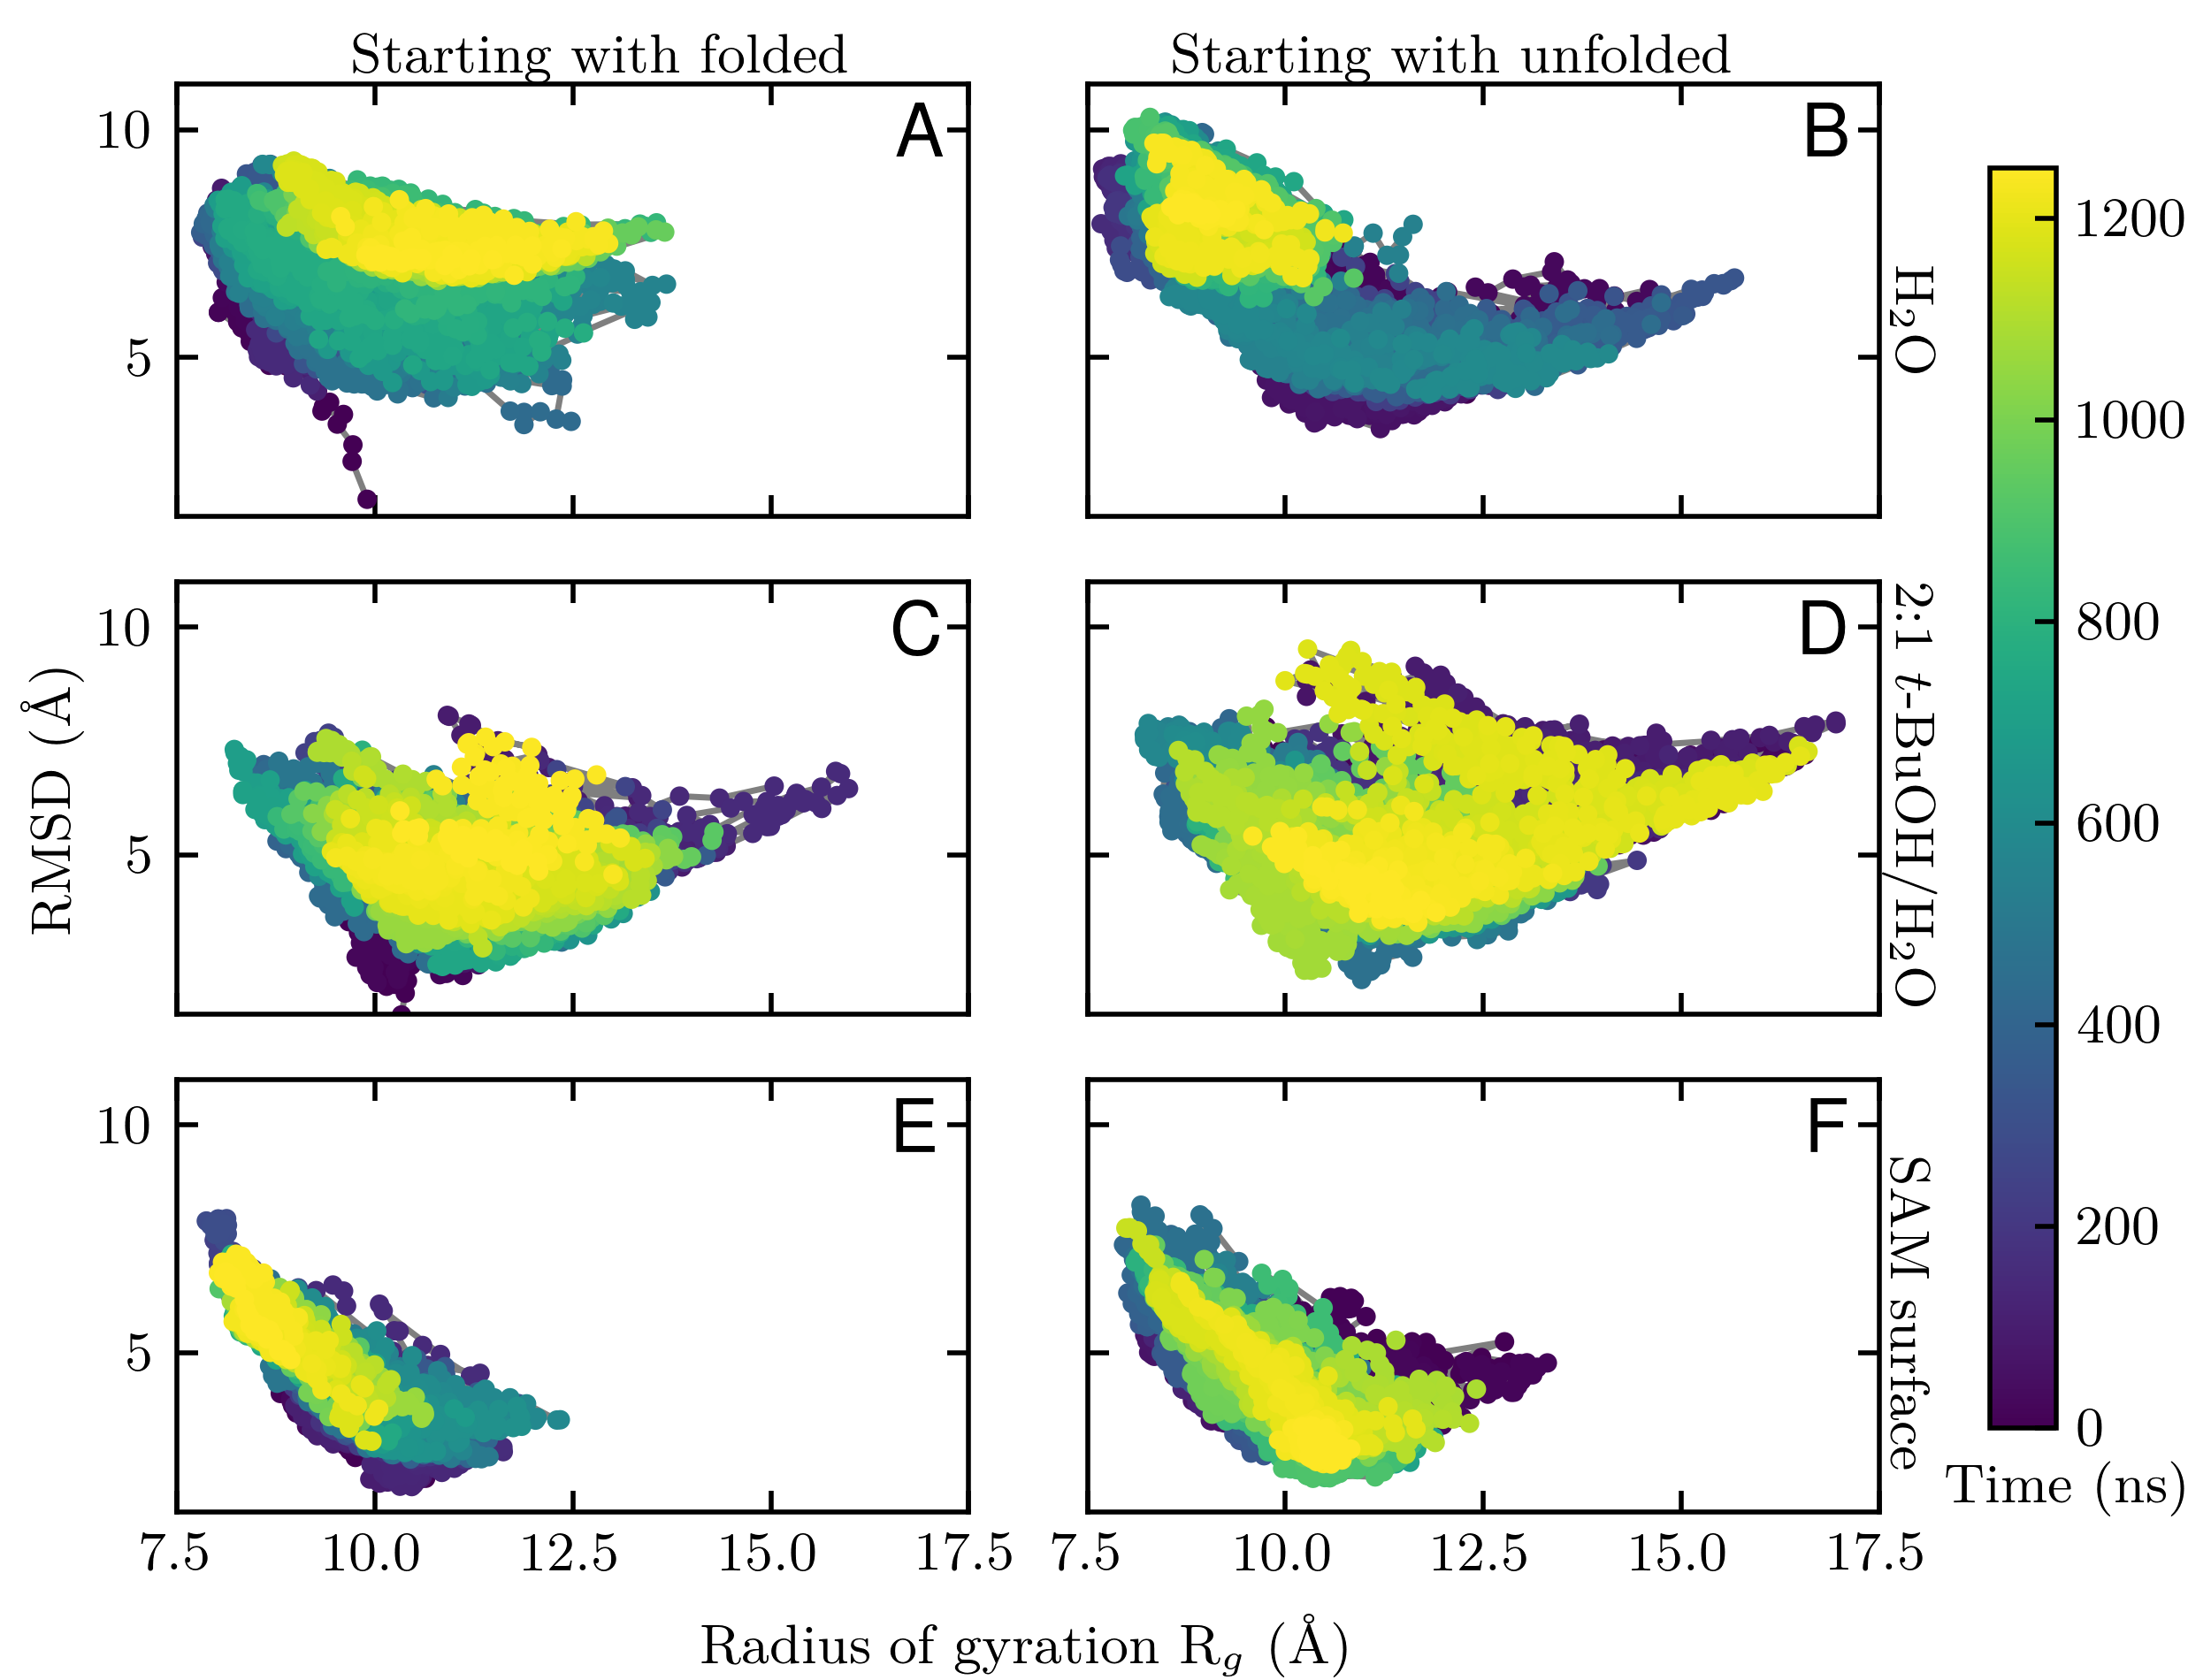
\includegraphics[width=6.0in]{figures-helix/combined_rgyr_v_rmsd.png}
    \caption{
        Conformational space sampled by \pep{} in six simulations. 
        On the $x$-axis is the radius of gyration of the protein. 
        On the $y$-axis is the backbone RMSD away from a perfectly folded \textalpha{}-helix. 
        Each point represents a 100 ps average and is colored by its time. 
        A, C, E: \pep{} began the simulation in an \textalpha{}-helical conformation. 
        B, D, F: \pep{} began the simulation unfolded. 
        A, B: the peptide was dissolved in water. 
        C, D: the peptide was dissolved in \tbawat{}. 
        E, F: the peptide was on the surface of a SAM dissolved in water.
    }
    \label{fig:helix-rgyr_v_rmsd}
\end{figure}

\subsection{Free energy analysis of folding}

In order to further investigate the preferential folding of \pep{} in \tbawat{} and on the surface of a SAM, we calculated the 2D free energy surface sampled in each environment. 
From the combined ensemble (the trajectory from the folded conformation and from the unfolded conformation, excluding snapshots prior to the equilibration times), we binned the calculated backbone RMSD from the \textalpha{}-helical conformation and $R_g$ (from Figure \ref{fig:helix-rgyr_v_rmsd}) and inverted the histogram according to eq \ref{eq:helix-boltz} using the gmx sham module:
\begin{equation}
    \Delta G = -k_B \ln(P)
    \label{eq:helix-boltz}
\end{equation}
where $\Delta G$ is the relative free energy of the bin, $k_B$ is the Boltzmann constant, and $P$ is the relative probability of the bin taken from the histogram. 
The calculated free energy surfaces are shown in Figures \ref{fig:helix-free_cluster}A-C, where $\Delta G$ of the unsampled regions were defined to be zero. 
The free energy surface (Figure \ref{fig:helix-free_cluster}A) of \pep{} in water displayed a free energy minimum ($\Delta G = -21.4$ kJ mol$^{-1}$) at high RMSD and low $R_g$, consistent with compact, non-helical conformations. 
In \tbawat{}, the free energy surface (Figure \ref{fig:helix-free_cluster}B) was shallower and more diffuse with a less distinct minimum ($\Delta G = -18.7$ kJ mol$^{-1}$), indicating partial destabilization of the most probable conformations. 
Conformations with high $R_g$ and low RMSD, consistent with extended, helical structures, were more stabilized in \tbawat{} than in water. 
On the surface of the SAM, the free energy surface (Figure \ref{fig:helix-free_cluster}C) favored conformations with low $R_g$ and low RMSD, consistent with compact, helical conformations. 
The minimum ($\Delta G = -22.5$ kJ mol$^{-1}$) had slightly higher RMSD to that in \tbawat{} with much lower $R_g$, and another minimum was apparent at lower RMSD and similar $R_g$ to that in \tbawat{}. 
Together, these results demonstrate that water stabilizes compact, non-helical conformations of \pep{}, \tbawat{} weakly stabilizes extended, helical conformations, and the SAM surface strongly stabilizes compact, helical conformations.

\begin{figure}
    \center
    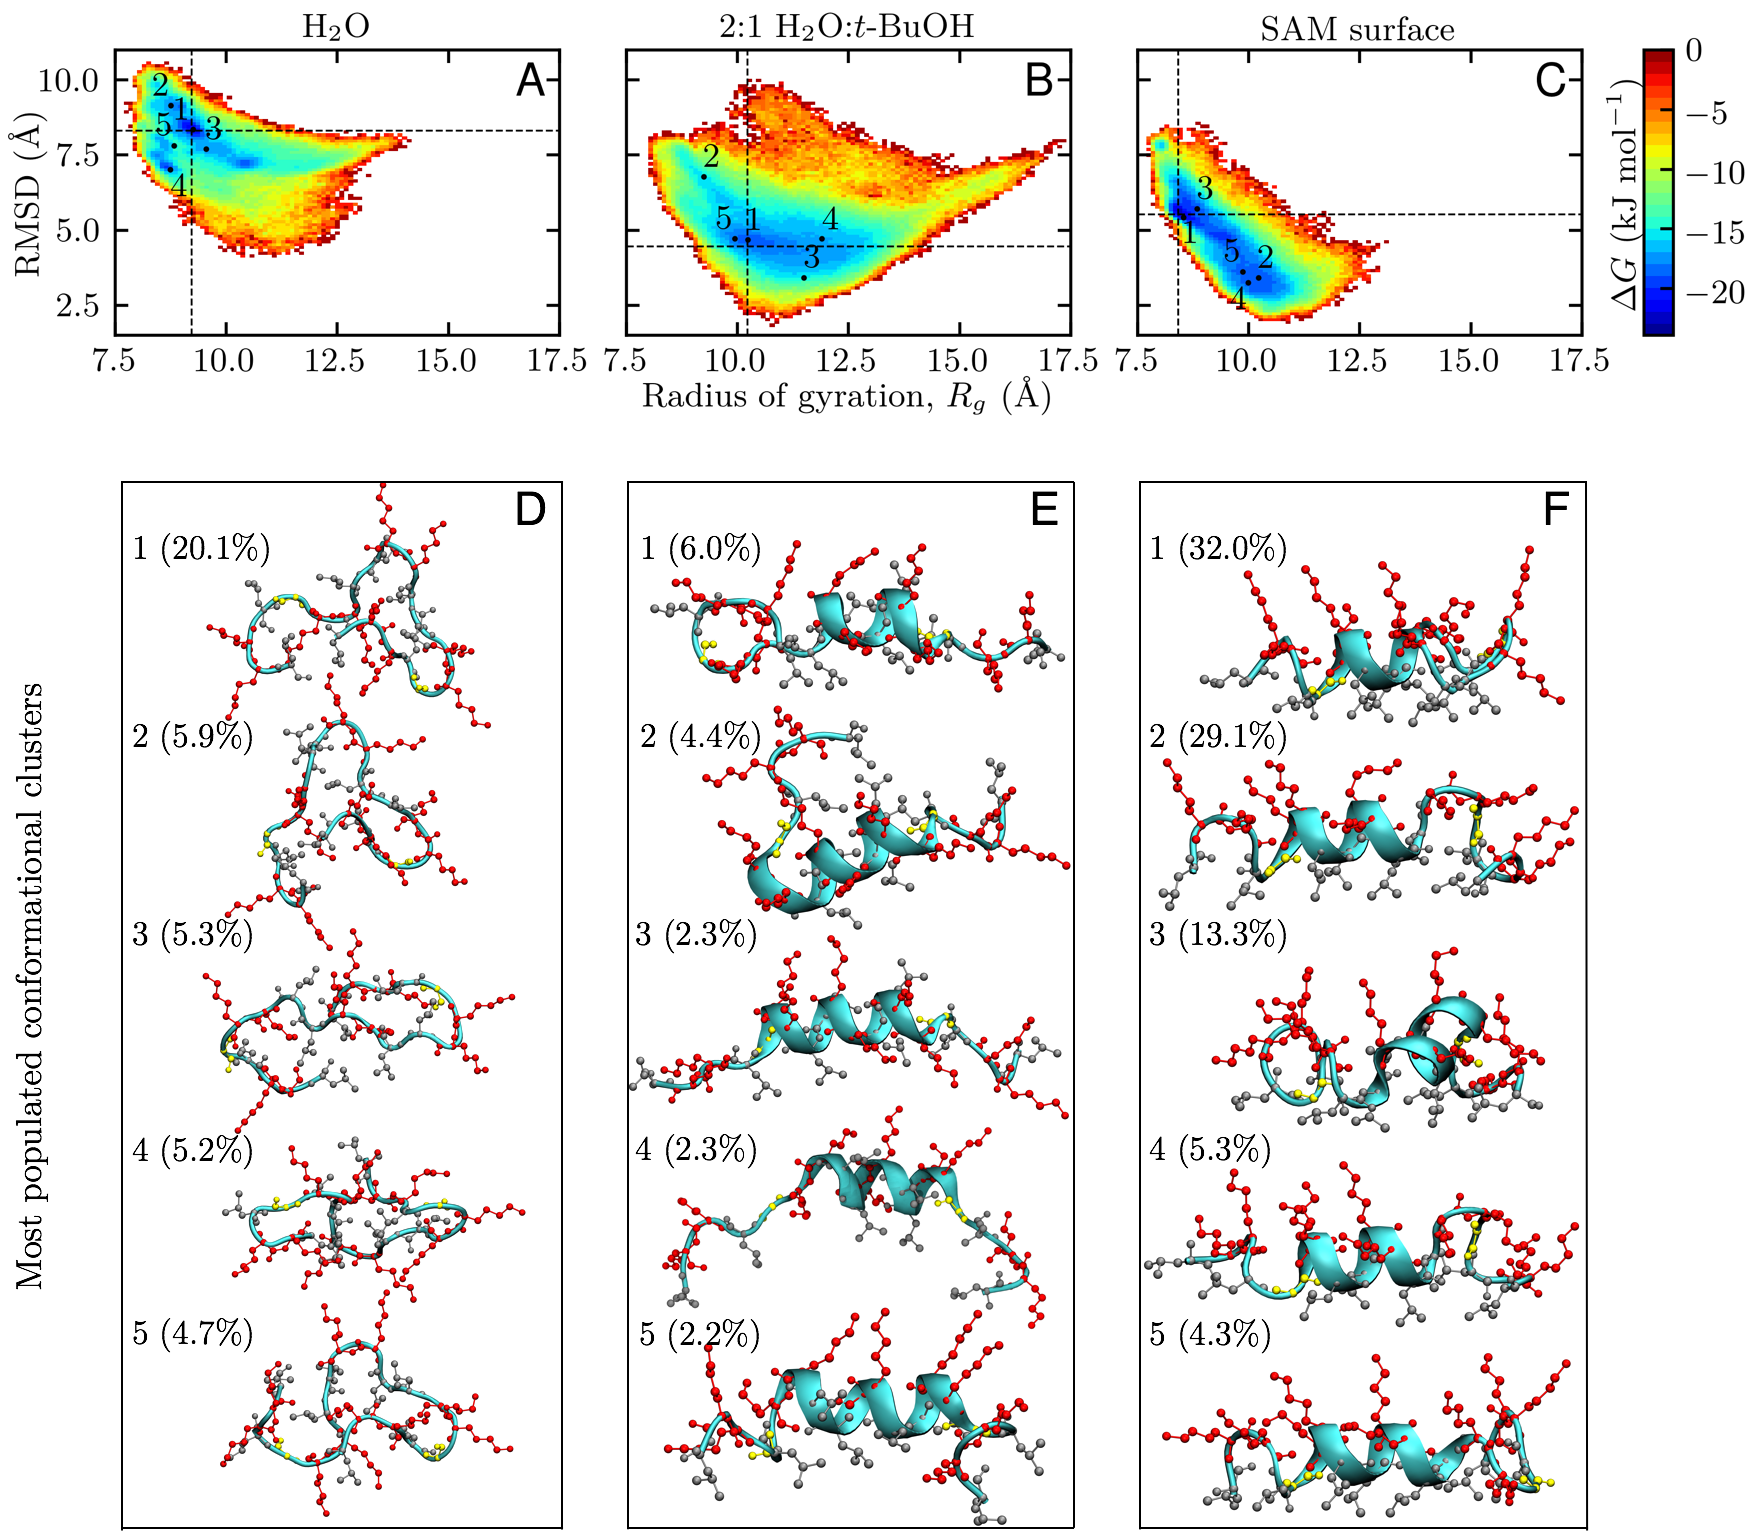
\includegraphics[width=5.50in]{figures-helix/clusters_revisions.png}
    \caption{
        A, B, C: Free energy surface of the combined ensemble of structures on \pep{} in the three solvent environments. 
        On the $x$-axis is the radius of gyration of the protein. 
        On the $y$-axis is the backbone RMSD away from a perfectly folded \textalpha{}-helix. 
        The intersection of the dashed lines is the global minimum for each surface. 
        D, E, F: Central structure from each of the top five conformation clusters from the combined ensemble of structures. 
        The central structure was taken from the frame with the lowest RMSD to all the other structures in the cluster. 
        The cyan ribbon represents the protein backbone, the red spheres represent the heavy atoms of the lysine residues, the gray spheres represent the heavy atoms of the leucine residues, and the yellow spheres represent the heavy atoms of the glycine residues. 
        Each structure is labeled with the percentage of the total number of structures that are less than 2.5 \si{\angstrom} backbone RMSD away from the structure shown. 
        A, D: the peptide was dissolved in water. 
        B, E: the peptide was dissolved in \tbawat{}. 
        C, F: the peptide was on the surface of a SAM dissolved in water.
    }
    \label{fig:helix-free_cluster}
\end{figure}

\subsection{Cluster analysis of most populated structures from the simulated ensembles}

To investigate the structures stabilized by the free energy surfaces discussed above, we performed a cluster analysis on the combined ensemble of structures for each of the three solvent environments. 
Because this requires pairwise RMSD calculations, structures were only sampled every 100 ps for this analysis. 
Clusters were identified using the Gromos algorithm\cite{Daura1999} and the gmx cluster module with a cutoff of 2.5 \si{\angstrom} backbone RMSD between clusters in order to visualize common structural motifs throughout the trajectory. 
Figure \ref{fig:helix-free_cluster}D illustrates the central structure of the five most populated conformational clusters of \pep{} in water. 
The central structure of the peptide was taken from the frame with the lowest RMSD from all the other structures in the cluster. 
The label indicates the percentage of the total ensemble of structures that were represented by the cluster. 
In water, all of the most populated clusters were disordered or unfolded conformations, and their $R_g$ and backbone RMSD to an \textalpha{}-helical conformation are labeled on the free energy surface in Figure \ref{fig:helix-free_cluster}A. 
None of the five clusters in water had helical character; 
the hydrophobic leucine residues (gray) were centrally located while the hydrophilic lysine residues (red) were more radially distributed and directed out into the surrounding solution. 
Further, a \textbeta{}-turn motif at the N-terminus, where the peptide turns back on itself and aligns in an anti-parallel fashion, was observed in all five clusters. 
While this motif was too short to be considered a \textbeta{}-strand by the DSSP algorithm and instead was classified as ``bend,'' these residues accounted for the $\sim$0.4 strand character observed in the stacked conformational fractions (Figure \ref{fig:helix-conf_fracs}A and \ref{fig:helix-conf_fracs}B).

Figure \ref{fig:helix-free_cluster}E illustrates the central structure of the five most populated conformational clusters of \pep{} in \tbawat{}, and the corresponding $R_g$ and RMSD of these structures are labeled on the free energy surface in Figure \ref{fig:helix-free_cluster}B. 
All five contained 2-3 helical turns in the middle region of the peptide. 
In contrast to the structures in water, the leucine residues (gray) appeared to be on the opposite side of the helical axis than the hydrophilic lysine residues (red). 
The two terminal regions did not have defined secondary structure. 
They were typically extended, and the residues were classified as ``coil'' by DSSP (Figure \ref{fig:helix-dssp}C and \ref{fig:helix-dssp}D). 
The top five clusters only accounted for 17.2\% of the total ensemble of structures, which implies a large amount of intrinsic disorder for the peptide in \tbawat{} and is consistent with the more diffuse free energy surface. 
Nevertheless, the stacked conformational fractions in Figures \ref{fig:helix-conf_fracs}C and \ref{fig:helix-conf_fracs}D and the DSSP assignments in Figures \ref{fig:helix-dssp}C and \ref{fig:helix-dssp}D demonstrate that the majority of the less populated clusters not shown in Figure \ref{fig:helix-free_cluster}E had similar secondary structure in the middle region of the peptide.

Finally, Figure \ref{fig:helix-free_cluster}F illustrates the central structure of the five most populated conformational clusters of \pep{} on the surface of the SAM, and the corresponding $R_g$ and RMSD of these structures are labeled on the free energy surface in Figure \ref{fig:helix-free_cluster}C. 
Again, all five of the clusters displayed 2-3 helical turns in the middle region of the peptide, and the leucine (gray) and lysine (red) residues were clearly separated from each other. 
For reference, these structures were oriented such that the SAM surface (not shown) was below the peptide, adjacent to the leucine residues. 
In contrast to the peptide in \tbawat{}, the terminal regions of the peptide at the SAM surface had high curvature. 
The residues in this region were classified as ``turn'' by the DSSP algorithm because they lacked the repeating hydrogen bonds to be classified as helical (Figures \ref{fig:helix-dssp}E and \ref{fig:helix-dssp}F). 
Furthermore, the five clusters shown in Figure \ref{fig:helix-free_cluster}F accounted for 84.0\% of the total ensemble of structures, which implies that the peptide on the surface was significantly more structured than in either of the two solutions.

A comparison of the coverage of the total ensemble of structures against the number of clusters is shown in Figure \ref{fig:helix-coverage}. 
The ensemble of structures of \pep{} on the SAM was covered by significantly fewer clusters than \pep{} in either solution, consistent with the distinct minima of $\Delta G$ apparent on the free energy surface. 
In turn, the ensemble of structures of \pep{} in \ce{H2O} was covered by fewer clusters than \pep{} in \tbawat{}. 
This is again consistent with the distinct minima with slightly higher $\Delta G$ apparent on the free energy surface of \pep{} in \ce{H2O} and with the diffuse free energy surface with the highest minimum $\Delta G$ for \pep{} in \tbawat{}. 
This implies that the structural regularity of \pep{} increased from \tbawat{}, to \ce{H2O}, to the SAM surface, revealing a particular advantage of complementing the experimental studies with MD simulations. 
Only the average structure may be observed in the bulk experimental CD spectra but the simulations reveal a dynamic distribution of structures that all contribute to the overall experiment. 

\begin{figure}
    \center
    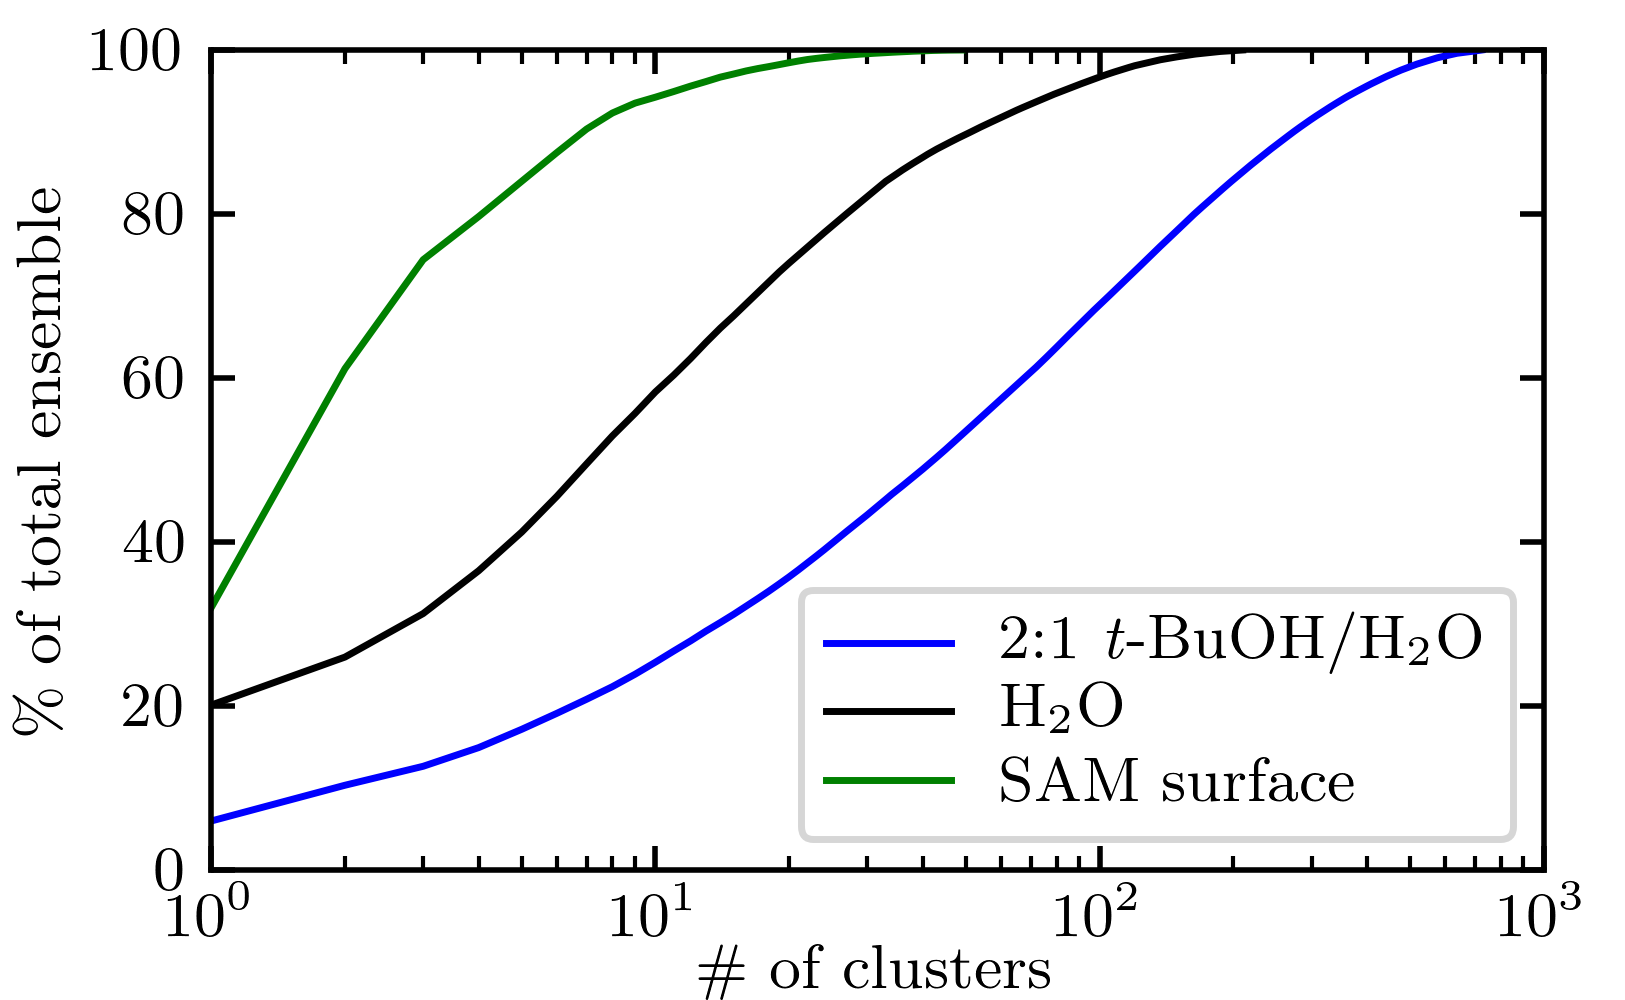
\includegraphics[width=3.25in]{figures-helix/clust-size.png}
    \caption{
        The percentage of coverage of the total ensemble of structures against the number of clusters for the peptide in water (black), in \tbawat{} (blue), and on the surface of a SAM (green).
    }
    \label{fig:helix-coverage}
\end{figure}

\subsection{Conformational fractions are consistent with experimental CD spectra}

While the central structures in Figure \ref{fig:helix-free_cluster} are consistent with our expectations from the experimental CD spectra in Figure \ref{fig:helix-cd_spectra}, it is not clear if the structural differences observed are enough to account for the change in the spectra. 
This is further complicated by the fact that conformations with large amounts of disorder, such as those of \pep{} in these three systems, do not always result in well-defined secondary structures that are apparent from CD spectroscopy. 
More advanced techniques, such as chiral sum frequency generation, can more quantitively determine the degree of each secondary structure exhibited by the peptide on biological surfaces\cite{Fu2011}. 
However, because of the wide spread use of CD as a measurement of secondary structure, we: 
1) compared the secondary structure calculated from the experimental spectra to the secondary structures from simulation; 
and 2) compared the calculated CD spectra from the MD trajectories to the experimental CD spectra. 
Although these comparisons have the same goal, each relies on different spectral analysis tools, and are thus two orthogonal ways to compare the experimental CD data to the calculated MD structures. 
In order to accomplish the first comparison strategy, we deconvoluted the experimental spectra into conformational fractions using the online deconvolution server BeStSel\cite{Micsonai2015, Micsonai2018}. 
This routine uses a basis set of CD spectra of proteins with known structure to estimate the fraction of secondary structures that would reconstitute the given CD spectrum. 
The spectra of the peptide in water and in \tbawat{} were input as is from Figure \ref{fig:helix-cd_spectra}, and good fits, with normalized RMSDs (NRMSDs) of less than 0.02, were obtained. 
However, for the spectrum of the peptide on the SAM surface (green spectrum in Figure \ref{fig:helix-cd_spectra}), we did not obtain an acceptable fit with the spectrum as shown. 
There were three reasons for this failure. 
First, the baseline of the spectrum was not consistent with the two spectra collected in solution. 
This created a significant amount of error since all of the BeStSel basis spectra have zero ellipticity at 250 nm. 
Second, the concentration of the peptide on the surface was not consistent with the other two experiments. 
The fits are highly dependent on accurate concentration estimates, since weak signals can occur from either poorly organized secondary structures or low concentrations of peptide. 
Third, the spectrum was red-shifted by 1 nm compared to the solution-phase spectra, probably due to the presence of the hydrophobic surface \cite{Chen1997}. 
The red-shift moved the characteristic transitions of \textalpha{}-helices to 209 and 223 nm, which caused the BeStSel algorithm to underestimate the amount of helical character. 
We therefore modified the experimental CD spectrum of \pep{} on the SAM surface in three ways: 
1) we corrected the baseline by forcing it to zero at 250 nm; 
2) we scaled the spectrum by a factor of 10 to account for the reduced concentration of the peptide on the surface compared to solution; and 
3) we blue-shifted the spectrum by 1 nm to place the absorption minima at 208 nm and 222 nm. 
A good fit for this corrected spectrum was obtained with NRMSD of less than 0.02. 

The average conformational fractions from the simulations (excluding the equilibration times discussed above) and the conformational fractions determined by BeStSel are shown in Table \ref{tbl:helix-frac_bestsel}. 
Fractions that differ by less than 0.05 are shown in bold. 
For \pep{} in water, the conformational fraction in simulation and from the BeStSel deconvolution were in strong agreement for the fraction of the peptide that was either in a helical (0.001 and 0.017, for simulation conformational fraction and BeStSel estimation respectively) or unfolded structure (0.527 and 0.550). 
However, the MD trajectories underestimated the fraction of strand character (0.042 and 0.188) and overestimated the fraction of turn character (0.430 and 0.245). 
This is consistent with investigations that demonstrated that OPLS can be biased toward extended and \textbeta{}-turn conformations\cite{Best2011, Smith2015}. 
For \pep{} in \tbawat{}, the conformational fractions were in good agreement for all four categories: helical (0.276 and 0.261), turn (0.130 and 0.150), strand (0.173 and 0.184), and unfolded (0.421 and 0.405). 
Finally, for \pep{} on the surface of the SAM, the conformational fractions in simulation and from the BeStSel deconvolution were in good agreement for the helical (0.318 and 0.278) and unfolded fractions (0.278 and 0.221). 
However, the simulations yielded a slightly higher turn fraction (0.296 and 0.197) and a slightly lower strand fraction (0.163 and 0.304) than the BeStSel estimates. 
There are two possible sources for this disagreement for the peptide at the SAM: 
1) there is a large amount of noise in the experimental data of the peak at 200 nm, which is due to the difficulty of taking such spectra on a surface; and 
2) there is greater error in estimating the concentration of the peptide on a surface than in solution. 
The accuracy of the BeStSel deconvolution is heavily dependent on both of these factors. 
A third possible source of this discrepancy could be again the choice of force field used in the simulations, as it has been suggested qualitatively that OPLS-AA may over represent random coil character on SAM surfaces\cite{Collier2012}. 
Since the onset of the present work, a new force field (CHARMM36m) has been shown to be accurate for intrinsically disordered peptides\cite{Huang2017}, which might ameliorate the discrepancies in Table \ref{tbl:helix-frac_bestsel}. 
We are investigating this in ongoing simulations using the CHARMM36m force field. 
Nevertheless, the agreement between the fractions from the deconvolution and the simulations is striking and gives us confidence in the accuracy of the simulations.

\begin{table}
    \caption{Average conformational fraction from simulation and conformational fractions from BeStSel\cite{Micsonai2015, Micsonai2018} CD spectra deconvolution.}
    \begin{center}
        \resizebox{6.0in}{!}{
    \begin{tabular}{c|cccc|cccc}
    \toprule
        Solvent        & \multicolumn{4}{c}{Calculated} & \multicolumn{4}{c}{BeStSel deconvolution from experiment} \\
        & Helix & Turn & Strand & Unfolded & Helix & Turn & $\beta$-sheet & Others \\
    \midrule
        \ce{H2O} & \textbf{0.001} & 0.042 & 0.430 & \textbf{0.527} & \textbf{0.017} & 0.188 & 0.245 & \textbf{0.550} \\
        2:1 \ce{H2O}:\emph{t}-BuOH & \textbf{0.276} & \textbf{0.130} & \textbf{0.173} & \textbf{0.421} & \textbf{0.261} & \textbf{0.150} & \textbf{0.184} & \textbf{0.405} \\
        SAM surface   & \textbf{0.318} & 0.296 & 0.163 & \textbf{0.223} & \textbf{0.278}* & 0.197* & 0.304* & \textbf{0.221}* \\
    \bottomrule
    \end{tabular}
}
    \end{center}
    \textbf{Bold} indicates that the calculated fraction is within $\pm 0.05$ of the BeStSel estimated counterpart. 
    *BeStSel deconvolution was performed on the CD spectrum of \pep{} on the SAM after applying a baseline correction, a 1 nm red-shift, and a scale-factor of 10. 
    See main text for details.
    \label{tbl:helix-frac_bestsel}
\end{table}

While the secondary structure estimated from the experimental spectra agreed with the simulations, we also calculated CD spectra from the MD trajectories in order to compare to experimental spectra (the second strategy described above). 
In order to accomplish this, we calculated the CD line spectrum for structures extracted every 100 ps in each of the six simulations using the DichroCalc portal \cite{Bulheller2009, Jasim2018}. 
Each line spectrum was convoluted with a Gaussian band shape using an in-house Python code to produce a continuous CD spectrum. 
We explored a range of bandwidths from 9 nm to 14 nm, but found that this did not change the observations and conclusions reported below (data not shown). 
Here, we show the spectra calculated with a bandwidth of 10 nm. 
The spectra were averaged across 125 ns time windows and are shown in Figure \ref{fig:helix-calc_cd}. 
For each simulation that started from a folded conformation (Figures \ref{fig:helix-calc_cd}A, \ref{fig:helix-calc_cd}C, and \ref{fig:helix-calc_cd}E), the first 125 ns averaged CD spectrum (dark blue trace) had a distinct minimum around 208 nm and 222 nm, a distinctive characteristic of the CD spectra of \textalpha{}-helices\cite{Holzwarth1965, Woody1967, Johnson1988, Berova2000circular, Kelly2005}.
For the simulation in water starting from a folded state (Figure \ref{fig:helix-calc_cd}A), these two minima disappeared as the peptide unfolded in solution, and then a positive peak appeared around 200 nm (green to yellow traces). 
This transition is associated with anti-parallel \textbeta{}-sheets\cite{Greenfield1969, Manning1988} and coincided with the appearance of strand character in the stacked conformational fraction (Figure \ref{fig:helix-conf_fracs}A). 
For the simulation in water starting from an unfolded state (Figure \ref{fig:helix-calc_cd}B), the two minima at 208 nm and 222 nm were present only weakly in the first few averaged spectra, when the peptide sampled some weakly helical configurations (Figure \ref{fig:helix-calc_cd}B). 
These two minima then disappeared and a positive peak at 200 nm appeared for the remainder of the trajectory. 
For the simulation in \tbawat{} starting from the folded state (Figure \ref{fig:helix-calc_cd}C), the two minima associated with \textalpha{}-helices (208, 222 nm) were present for each averaged window. 
The spectra were relatively consistent in each window with only minor changes in the intensity of the peaks. 
For the simulation in \tbawat{} starting from the unfolded state (Figure \ref{fig:helix-calc_cd}D), the first window averaged spectrum (0-125 ns, dark blue trace) had a positive peak around 200 nm. 
The positive peak disappeared in subsequent windows, replaced by two weak negative peaks around 208 nm and 222 nm. 
These two negative peaks grew in intensity until 1 \textmu{}s. 
The peptide then sampled some unfolded configurations (Figure \ref{fig:helix-conf_fracs}D), resulting in a final window averaged spectrum that had very weak minima at 208 and 222 nm (Figure \ref{fig:helix-calc_cd}D, yellow trace). 
Nevertheless, the majority of the spectra for the simulation of \pep{} in \tbawat{} had minima at 208 nm and 222 nm. 
For the simulation on the surface of the SAM starting from the folded state (Figure \ref{fig:helix-calc_cd}E), the window averaged CD spectra all had characteristic minima at 208 and 222 nm, with stronger intensity than that of the peptide in \tbawat{}, indicating more helical character. 
For the simulation on the surface of the SAM starting from the unfolded state (Figure \ref{fig:helix-calc_cd}F), all window averaged CD spectra had the same minima. 
The spectrum for 0-125 ns (dark blue trace) had the weakest minimum, since the peptide in this window was still folding. 
In subsequent windows, the strength of the minima tended to increase, again greater than the spectra of \pep{} in \tbawat{}.

\begin{figure}
    \center
    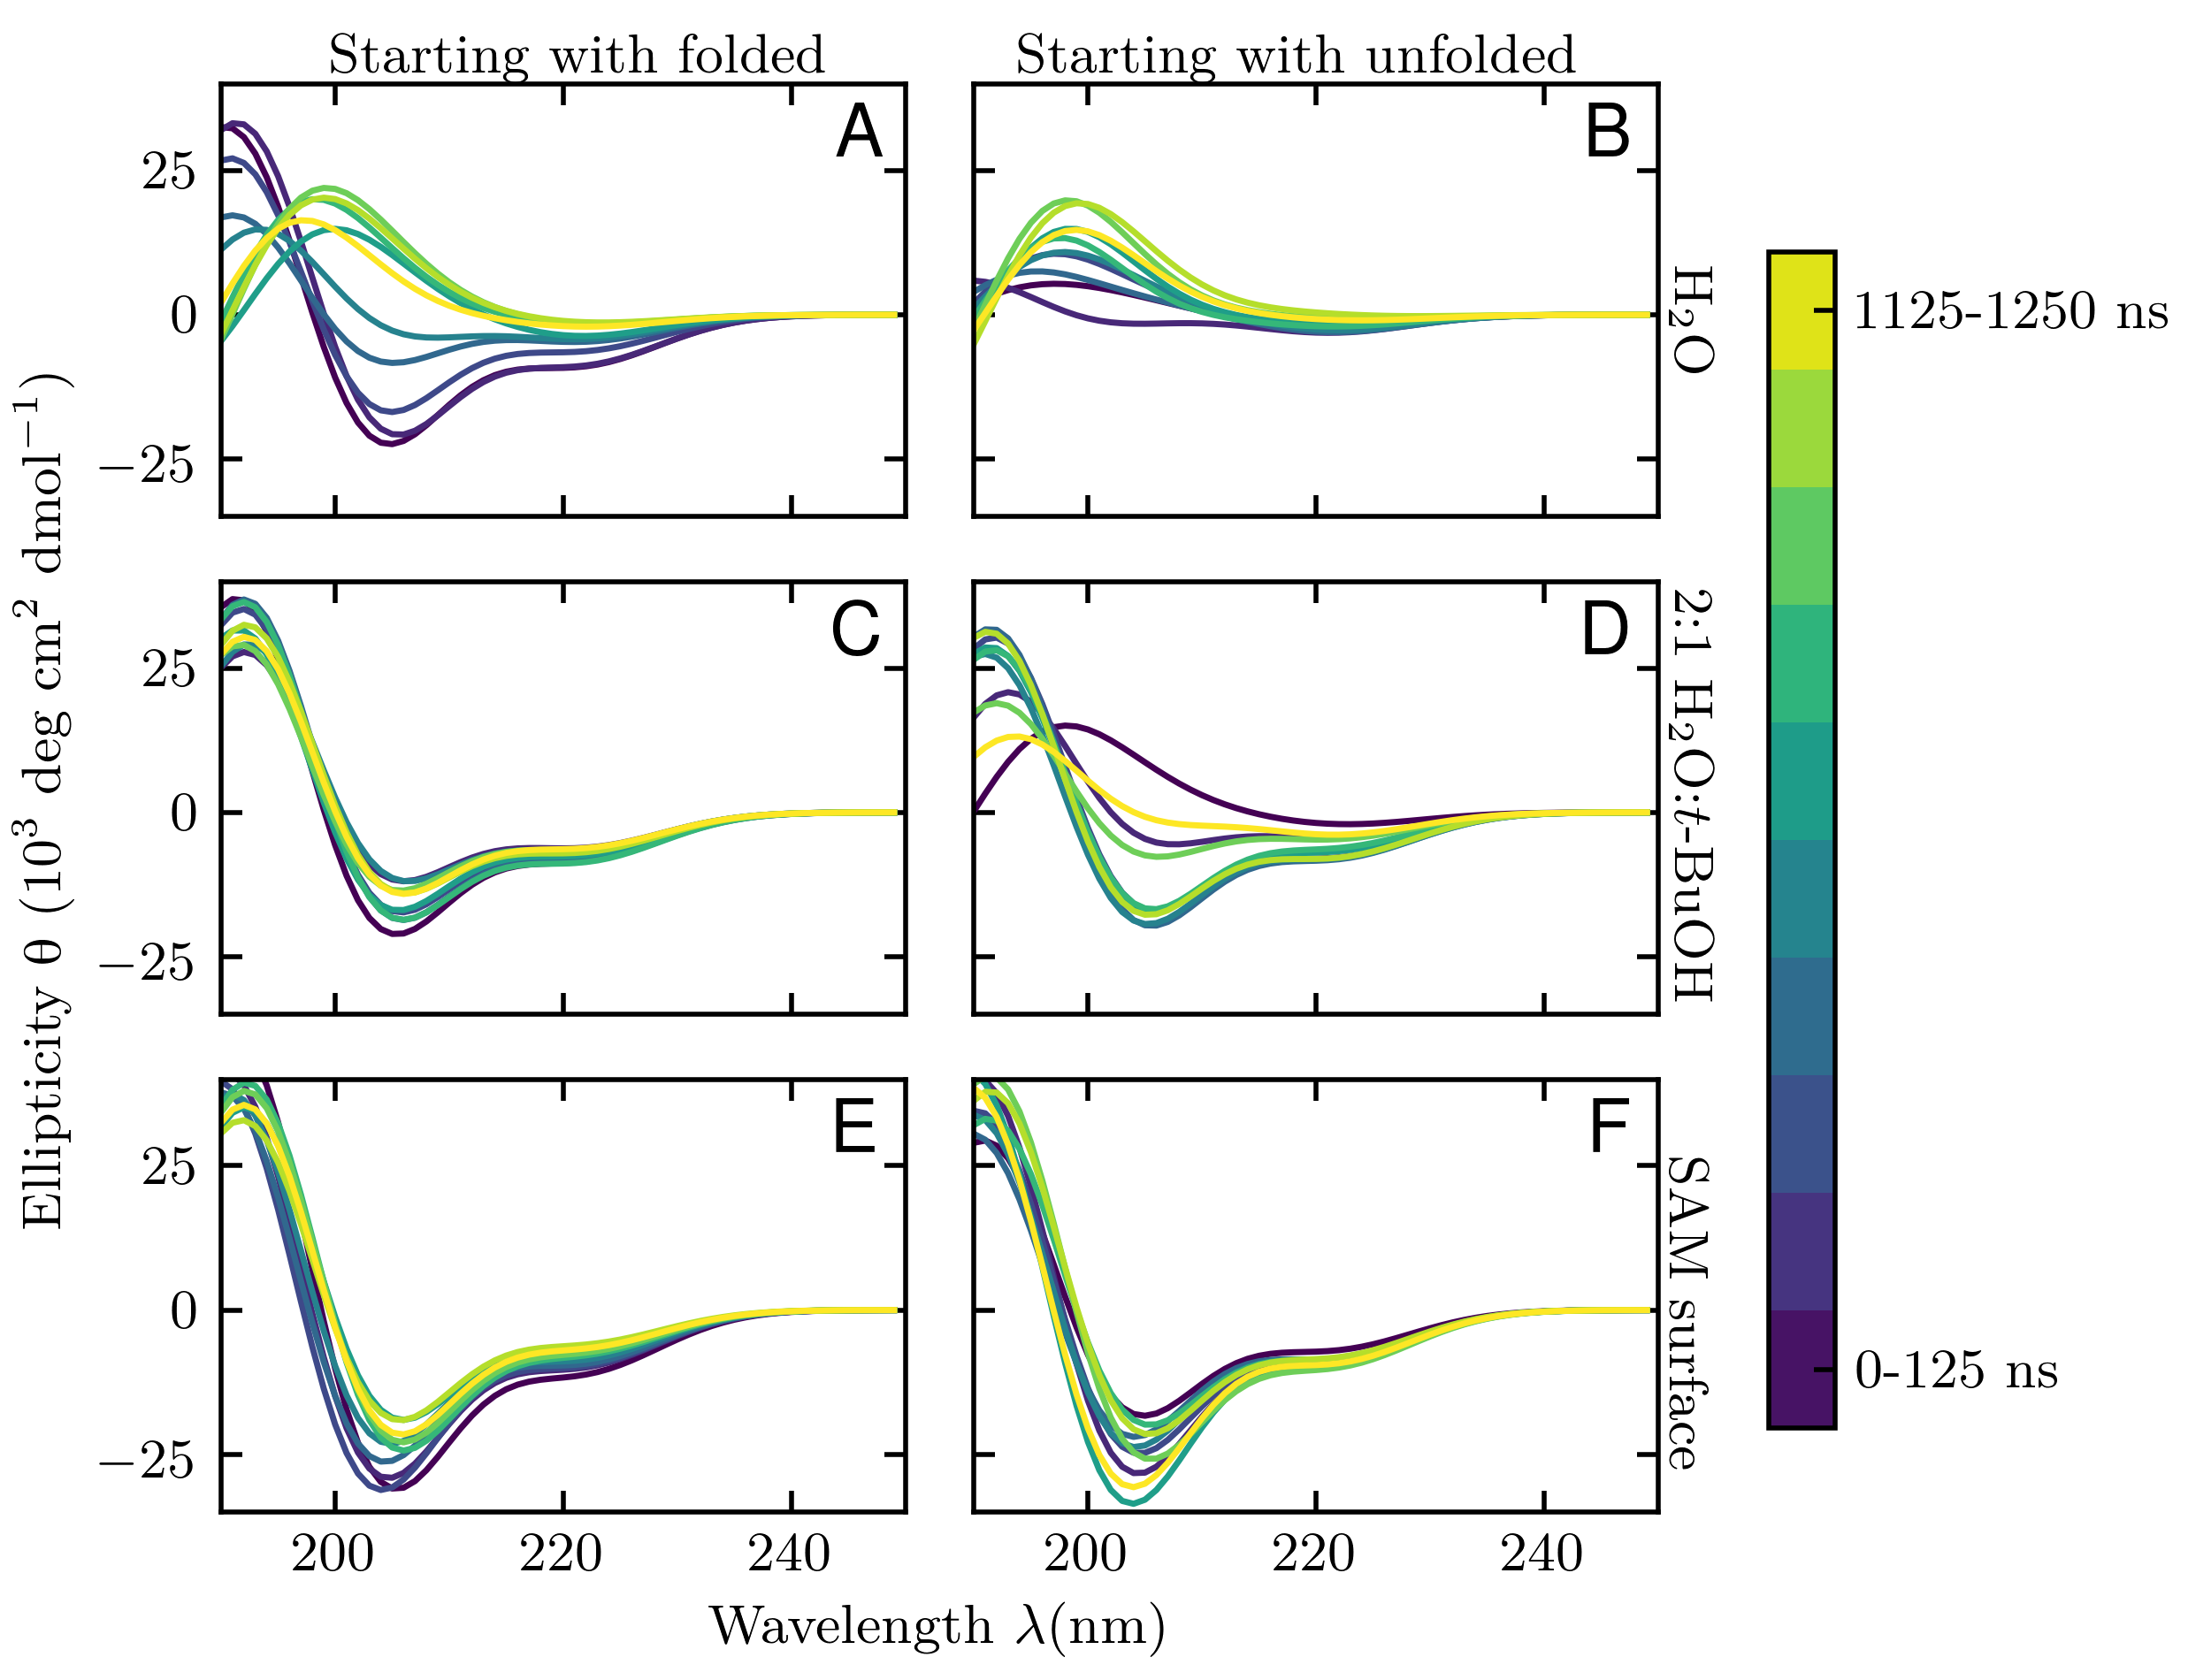
\includegraphics[width=6.0in]{figures-helix/cd_spectra_hirst_time_resolved.png}
    \caption{
        Computed CD spectra calculated from the MD trajectories using the DichroCalc portal and the Hirst basis set \cite{Hirst1998, Besley1999}.
        Each spectrum was convoluted with a Gaussian function with bandwidth of 10 nm. 
        Spectra were calculated every 100 ps, and each line represents a 125 ns average and is colored by its time. 
        A, C, E: \pep{} began the simulation in an \textalpha{}-helical conformation. 
        B, D, F: \pep{} began the simulation unfolded. 
        A, B: the peptide was dissolved in water. 
        C, D: the peptide was dissolved in \tbawat{}. 
        E, F: the peptide was on the surface of a SAM dissolved in water.
    }
    \label{fig:helix-calc_cd}
\end{figure}

The total averaged spectrum from the entire ensemble of structures in each solvent (excluding the equilibration times discussed above) are shown in Figure \ref{fig:helix-avg_cd}A. 
For the averaged spectrum of \pep{} in water (Figure \ref{fig:helix-avg_cd}A, black), there was a positive peak around 200 nm, and a very weak minimum at 222 nm. 
The positive peak was a result of the strand character and was not consistent with the experimental spectrum (Figure \ref{fig:helix-cd_spectra}, black). 
While this may be a result of our simulations slightly overestimating the strand character of \pep{} in water, the CD spectra of \textbeta{}-sheets are extremely sensitive to the exact configuration of the structure, and minor differences in the alignment of the \textbeta{}-sheet can result in large differences in the observed spectrum \cite{Micsonai2015}.
The difference in the computed spectrum and the experimental spectrum, therefore, may be due only to minor differences in the tilt of the \textbeta{}-sheet. 
However, both the computed and experimental spectra indicated no helical character, which was borne out in the simulations. 
For the computed spectrum of \pep{} in \tbawat{} (Figure \ref{fig:helix-avg_cd}A, blue), there were distinct negative transitions at 208 and 222 nm indicative of helical character. 
The computed spectrum was in good qualitative agreement with the experimental spectrum (Figure \ref{fig:helix-cd_spectra}, blue). 
Finally, the computed spectrum \pep{} on the surface of the SAM (Figure \ref{fig:helix-avg_cd}A, green) contained these same two negative peaks with greater intensity. 
While the absolute intensities in the experimental spectra cannot be compared to each other because of the difficulty in determining the concentration on the surface, the resolution of the two peaks in the experimental spectrum implied stronger helical character (Figure \ref{fig:helix-cd_spectra}, green). 
This was indeed captured by the computed spectrum. 
The relative intensity between the two peaks, however, was not captured, which could be due to the choice of the Hirst basis set\cite{Hirst1998, Besley1999} for the calculation. 
CD spectra computed using the Woody basis set\cite{Woody1999} shown in Figure \ref{fig:helix-avg_cd}B qualitatively matched the experimental spectrum for \pep{} on the SAM surface. 
However, the spectra calculated using this basis set failed to capture the relative intensity of the two peaks for \pep{} in \tbawat{}. 
Taken together, however, the calculated CD spectra were in qualitative agreement with the experimental spectra, which, when combined with the quantitative agreement of the conformational fractions from simulation and the BeStSel deconvolution, gives us confidence that we can accurately simulate the peptide in these complex environments.

\begin{figure}
    \center
    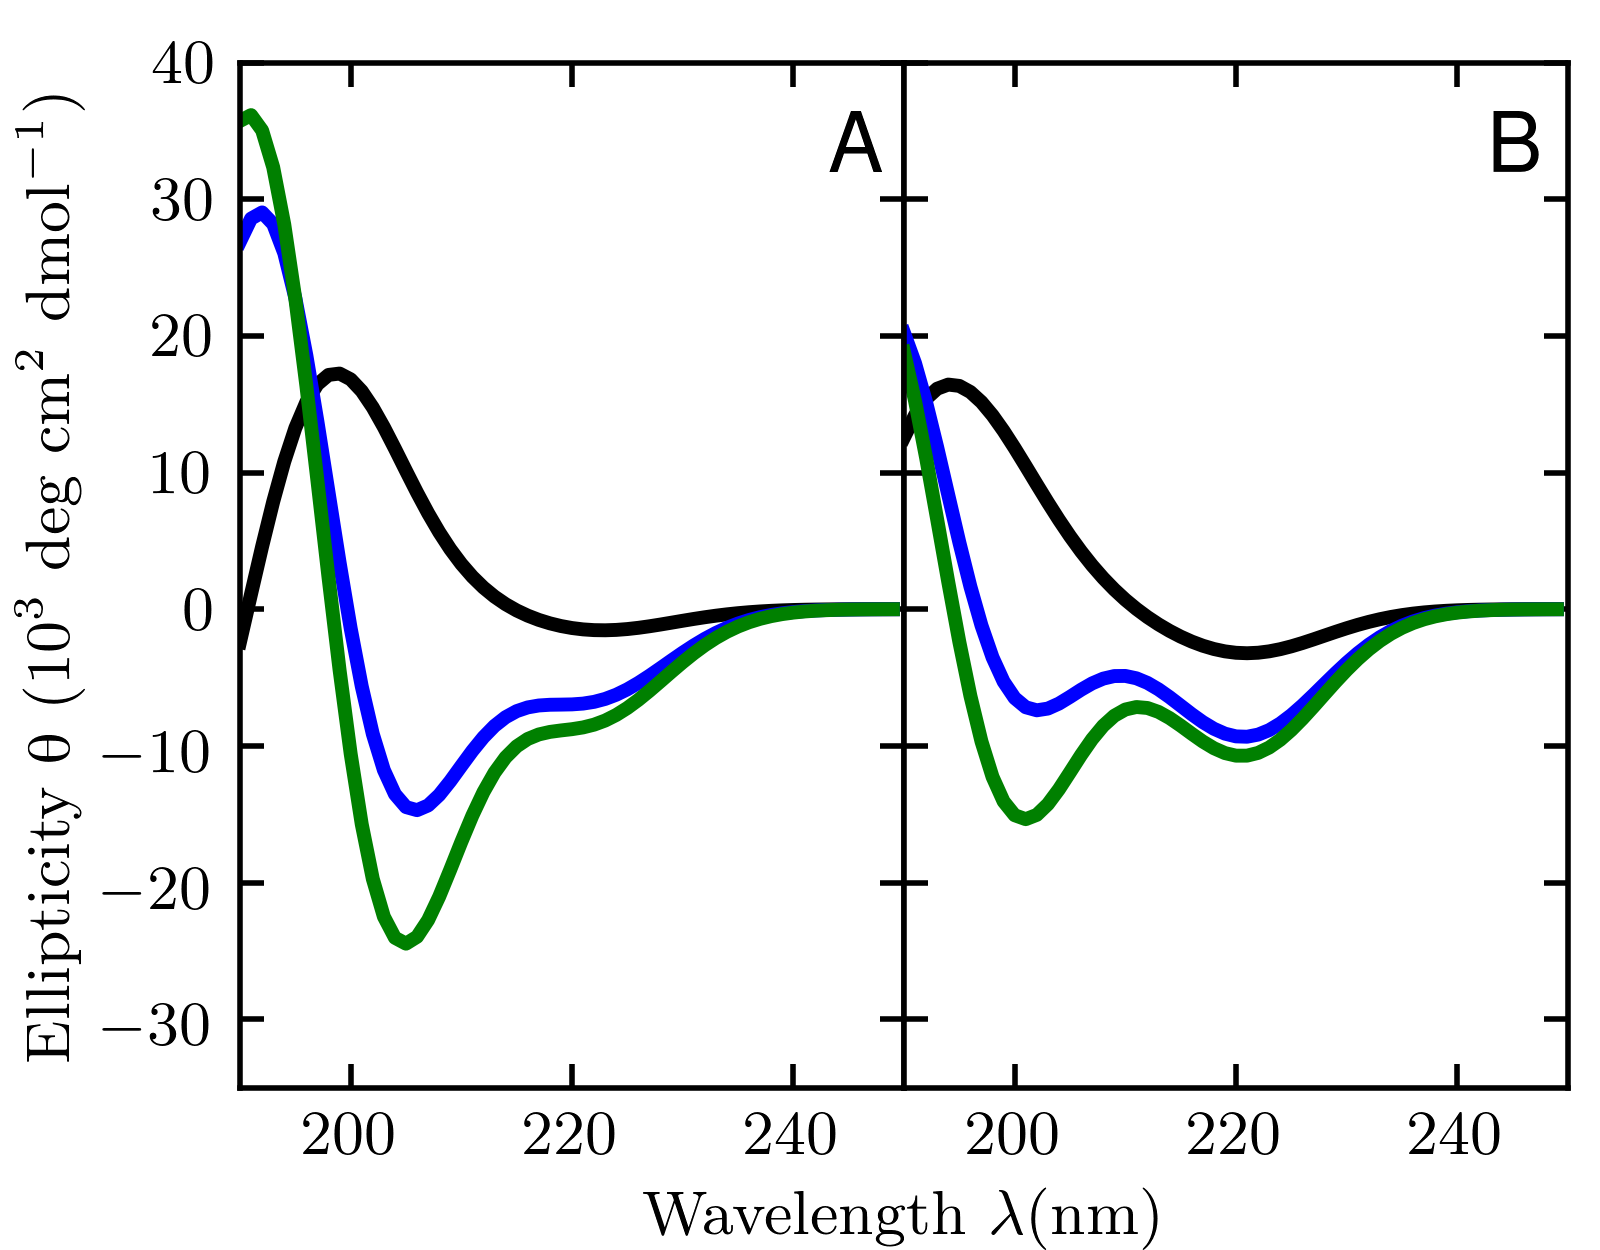
\includegraphics[width=3.25in]{figures-helix/combined_cd_spectra.png}
    \caption{
        Ensemble averaged CD spectra computed from MD simulations of \pep{} in water (black), \tbawat{} (blue), and on the surface of a SAM (green). 
        Spectra were computed using the DichroCalc web portal and either the Hirst basis set\cite{Hirst1998, Besley1999} (A) or the Woody basis set\cite{Woody1999} (B).
    }
    \label{fig:helix-avg_cd}
\end{figure}

%%%%%%%%%%%%%%%%%%%%%%%%%%%%%%%%%%%%%%%%%%%%%%%%%%%%%%%%%%%%%%%%
%%%%%%%%%%%%%%%%%%%%%%%%%%%%%%%%%%%%%%%%%%%%%%%%%%%%%%%%%%%%%%%%
\section{Discussion}\index{helix-discussion}
%%%%%%%%%%%%%%%%%%%%%%%%%%%%%%%%%%%%%%%%%%%%%%%%%%%%%%%%%%%%%%%%
%%%%%%%%%%%%%%%%%%%%%%%%%%%%%%%%%%%%%%%%%%%%%%%%%%%%%%%%%%%%%%%%

Our results demonstrate that the widely available OPLS-AA force field can accurately model our charged peptide \pep{} in these two complex environments: 
1) in a binary solvent (\tbawat{}); and 
2) on a SAM surface. 
The agreement between simulations that started at different conformations (folded and unfolded) showed that our results are not heavily influenced by our starting structure. 
The accuracy of these structures was demonstrated by: 
1) the quantitative agreement between the simulated conformational fractions and the fractions estimated by BeStSel deconvolution (Table \ref{tbl:helix-frac_bestsel}); and 
2) the qualitative agreement between the spectra computed from MD trajectories using DichroCalc (Figure \ref{fig:helix-avg_cd}) and the experimental spectra (Figure \ref{fig:helix-cd_spectra}). 
In particular, conformational transitions between helical and \textbeta{}-sheet structures have profound implications on amyloid plaque diseases such as Alzheimer's, Parkinson's, and Huntington's diseases\cite{Jahn2006, Chiti2009, Abedini2009, Hoop2016, Kim2016, Mondal2019}, particularly when the conformational change is induced by an interface \cite{Chi2010, Moores2011, Ho2018}. 
Here, we have shown that \pep{} switches between a \textbeta{}-turn motif in water, a partially folded helix in \tbawat{}, and a folded helix on a hydrophobic surface, demonstrating the utility of this model peptide for research into the molecular mechanisms of such diseases. 
Accurate simulations are paramount to this effort. 
Further, the conformational changes observed in simulation can guide experimental strategies to incorporate biomolecules on surfaces and provide foundational knowledge on the stability of protein structures in such environments.

Because of the unique sequence of our peptide that was designed to fold at a polar/apolar interface, the results presented here should not be used to assume that OPLS will be able to accurately model all conformational changes on a surface. 
The accuracy of any force field on a peptide in such an environment must be validated against experimental data. 
Nevertheless, the accuracy demonstrated here allows us to test specific mechanistic questions about how this peptide interacts with different surface environments. 
For example, in order to keep the peptide near the surface during the equilibration and heating processes, harmonic restraints were added to hold the glycine residues to the appropriate distance from the SAM. 
For the simulations discussed above, these restraints were removed for the production phase simulations, so that the peptide was unrestrained on the surface. 
However, in the experiment to which we are comparing our results, the peptide is covalently bound to the SAM through a triazole linker (Figure \ref{fig:helix-linker}). 
We do not have any experimental evidence to determine whether the peptide folds before reacting with the SAM layer, or if the peptide reacts and then folds. 
Further, the SAMs in these simulations were nearly perfectly ordered but by relaxing this, the effect of the order of the SAM on the peptide structure can now be tested \emph{in silico}. 
Below, we introduce two additional sets of simulations that test these experimental questions: 
1) the influence of the number of binding sites holding the peptide near the SAM surface on the folding process; and 
2) the effect of structural order of the SAM on the equilibrium structure of the peptide. 
Using these two additional sets of simulations, we identify two hypotheses regarding the mechanistic details of the peptide folding on the surface that can be specifically tested by experiment. 

In order to test the effect of the number of binding sites holding the peptide to the SAM surface, we ran four additional 1.25 \textmu{}s simulations where one or both of the harmonic restraints that bind the glycine residues to the SAM (see Section \ref{helix-anneal}) were kept for the production phase, instead of removing them as in the simulations reported above. 
The stacked conformational fractions for these additional simulations are shown in Figure \ref{fig:helix-bounds}, and the quantitative results (not including values before the 150 ns equilibration time) are shown in Table \ref{tbl:helix-bounds}. 
With both glycine residues bound, starting from a folded state (Figure \ref{fig:helix-bounds}A), the peptide remained folded through the entire simulation with average conformational fractions consistent with the unrestrained simulations shown in Table \ref{tbl:helix-frac_bestsel} (helix: 0.272, turn: 0.290, strand: 0.205, and unfolded: 0.233). 
However, starting from an unfolded conformation (Figure \ref{fig:helix-bounds}B), the peptide did not fold to the same extent, resulting in very different conformational fractions (helix: 0.083, turn: 0.083, strand: 0.350, and unfolded: 0.484). 
In contrast, with only one glycine bound (Figures \ref{fig:helix-bounds}C and \ref{fig:helix-bounds}D), the peptide reached similar conformational fractions from the folded state (helix: 0.278, turn: 0.264, strand: 0.179, and unfolded: 0.280) as from the unfolded state (helix: 0.275, turn: 0.315, strand: 0.162, and unfolded: 0.248). 
In both of these simulations, the average conformational fraction was consistent with the conformational fractions of the simulations with no restraints (Table \ref{tbl:helix-frac_bestsel}). 
Indeed, in every simulation of \pep{} on the SAM surface, the average conformational fractions were consistent \emph{except} when the peptide was unfolded and restrained at both glycine residues. 
These results imply that the two restraints prevent the peptide from folding. 
This in turn suggests the hypothesis that the peptide must be folded before the second covalent attachment occurs. 
We are currently testing this hypothesis experimentally. 

\begin{figure}
    \center
    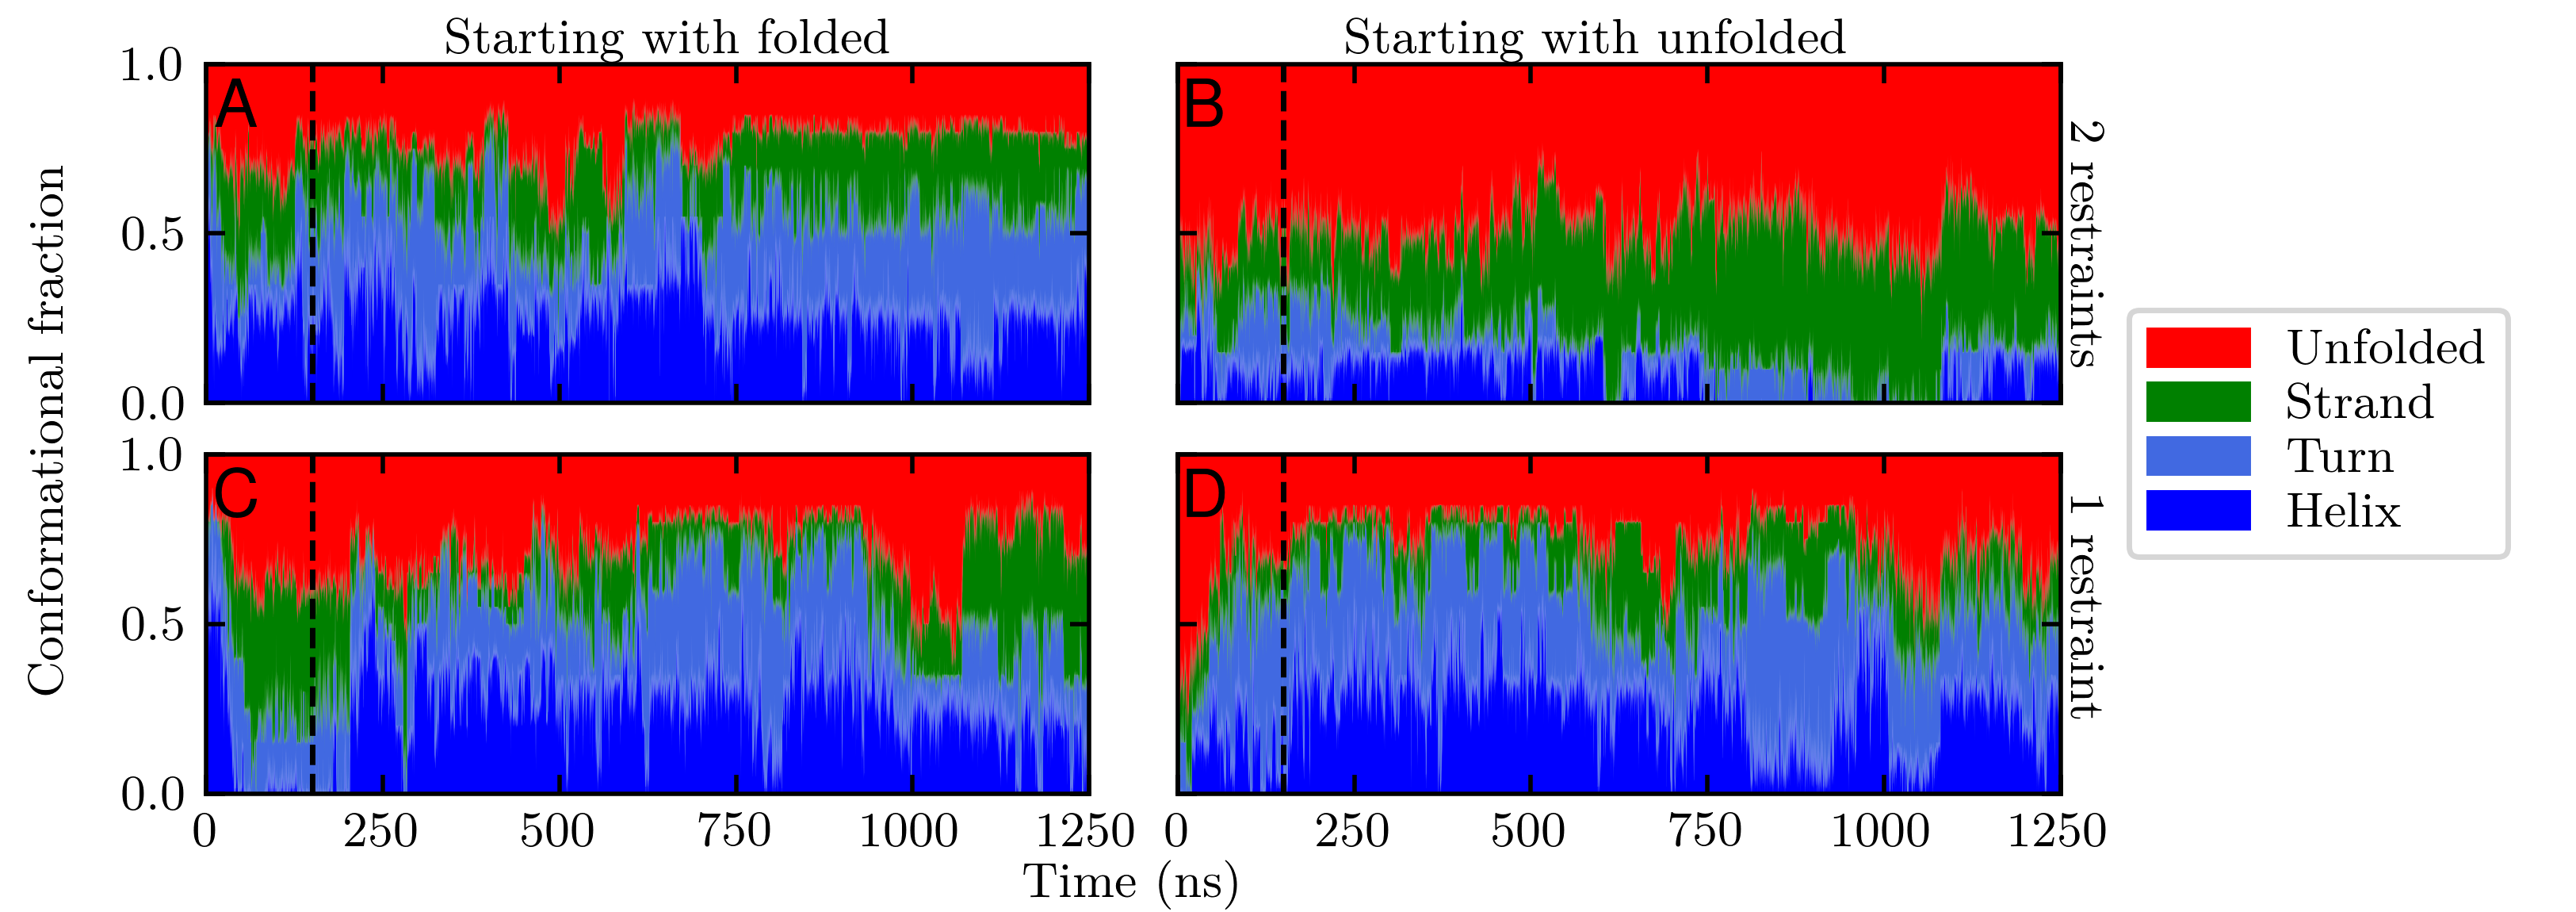
\includegraphics[width=6.0in]{figures-helix/bounds_helicity.png}
    \caption{
        Stacked conformational fractions of \pep{} on the surface of SAM from additional simulations in which either one or both glycine residues were harmonically restrained to the SAM. 
        A, C: \pep{} began the simulation in an \textalpha{}-helical conformation. 
        B, D: \pep{} began the simulation unfolded. 
        A, B: \pep{} was harmonically restrained to the SAM at both glycine residues. 
        C, D: \pep{} was harmonically restrained to the SAM at only one of the glycine residues. 
        The black dashed lines represent the equilibration time. 
        The data after this mark was averaged and is presented in Table \ref{tbl:helix-bounds}.
    }
    \label{fig:helix-bounds}
\end{figure}

\begin{table}
    \caption{Average conformational fractions from simulations of \pep{} on the surface of a SAM in which either one or both of the glycine residues in the peptide are harmonically restrained to the SAM.}
    \begin{center}
     \resizebox{6.0in}{!}{
     \begin{tabular}{c|cccc|cccc}
    \toprule
    Number of  & \multicolumn{4}{c}{From folded} & \multicolumn{4}{c}{From unfolded} \\
    harmonic restraints & Helix & Turn & Strand & Unfolded & Helix & Turn & Strand & Unfolded \\
    \midrule
    2 & 0.272 & 0.290 & 0.205 & 0.233 & 0.083 & 0.083 & 0.350 & 0.484 \\
    1 & 0.278 & 0.264 & 0.179 & 0.280 & 0.275 & 0.315 & 0.162 & 0.248 \\
    \bottomrule
    \end{tabular}
    }
    \end{center}
    \label{tbl:helix-bounds}
\end{table}

In order to investigate the effect of greater structural disorder within the SAM on the equilibrium structure of the surface-bound peptide, we loosened the harmonic restraints on the decanethiol molecules to $10^3$ kJ mol$^{-1}$ nm$^{-2}$ during the annealing stage of the system preparation (as opposed to $10^7$ kJ mol$^{-1}$ nm$^{-2}$ used for the preparation of the simulations above). 
This allowed molecules within the SAM to shift during the annealing and resulted in a slightly more disordered SAM surface. 
An illustration of the ``ordered'' and ``disordered'' SAMs are shown in Figure \ref{fig:helix-disordered_sam}A and \ref{fig:helix-disordered_sam}B, respectively, along with a density profile of the two surfaces in Figure \ref{fig:helix-disordered_sam}C. 
For the ordered SAM, sharp peaks in the density profile indicate the repetitive pattern of the sulfur and each carbon atom in the decanethiol over the entire SAM structure. 
When the restraints were loosened, the atoms of the SAM shifted during the annealing stages, resulting in a less well defined density profile, and indicating a more disordered SAM. 
In order to determine the effect of this disordered structure on the resulting fold of the surface-bound peptide, the simulations using this disordered SAM were run with harmonic restraints between the SAM and both, one, or none of the peptide's glycine residues for 1.25 \textmu{}s each. 
The stacked conformational fractions of these trajectories using a disordered SAM are shown in Figure \ref{fig:helix-disorder}. 
The averaged conformational fractions (not including the fractions before the equilibration time) are shown in Table \ref{tbl:helix-disorder}. 
Starting from a folded conformation and restrained to the SAM at both glycine residues (Figure \ref{fig:helix-disorder}A), the peptide remained folded for the entire trajectory, resulting in high helical content and conformational fractions consistent with the previous simulations on the ordered SAM surface (helix: 0.322; turn: 0.218; strand: 0.159; and unfolded: 0.302). 
However, starting from the unfolded state with two restraints (Figure \ref{fig:helix-disorder}B), the peptide did not fold and displayed low helicity (helix: 0.052; turn: 0.156; strand: 0.291; and unfolded: 0.501). 
The lack of agreement between these two simulations from simulation times that produced consistent results with unrestrained peptide reinforces our previous hypothesis; the second covalent attachment adds a large energy barrier between the folded and unfolded states that prevents the peptide from folding (or unfolding) on the SAM surface, and that \pep{} likely folds before the second bond to the SAM is formed.

\begin{figure}
    \center
    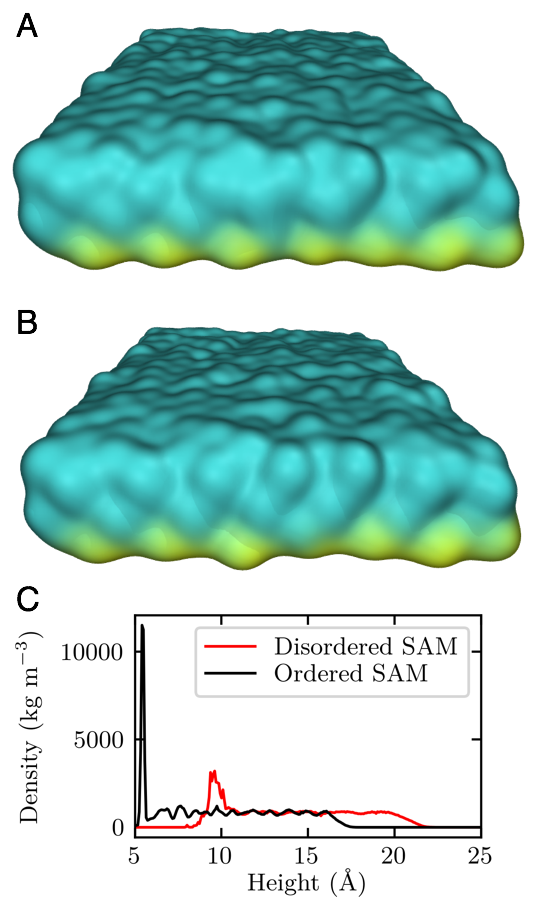
\includegraphics[width=3.25in]{figures-helix/order_figures.png}
    \caption{
        Surface filling representations of the more ordered SAM (A) used for the simulations with data presented in Figures \ref{fig:helix-conf_fracs}-\ref{fig:helix-bounds} and Tables \ref{tbl:helix-frac_bestsel}-\ref{tbl:helix-bounds} and of the more disordered SAM (B) used for the simulations with data presented in Figure \ref{fig:helix-disorder} and Table \ref{tbl:helix-disorder}. 
        Note that in the disordered SAM there is greater variation of height, leading to troughs that were observed to ``pull'' leucine residues, breaking the hydrogen bonding of the peptide backbone and destabilizing the helix. 
        (C) Density profiles in the $z$-dimension of the two different SAMs. 
        Note that the ordered SAM (black) has one tall peak corresponding to the position of the sulfur atoms, followed by ten distinct peaks that correspond to the positions of the ten carbon atoms. 
        These peaks are much more difficult to discern for the disordered SAM (red).
    }
    \label{fig:helix-disordered_sam}
\end{figure}

\begin{figure}
    \center
    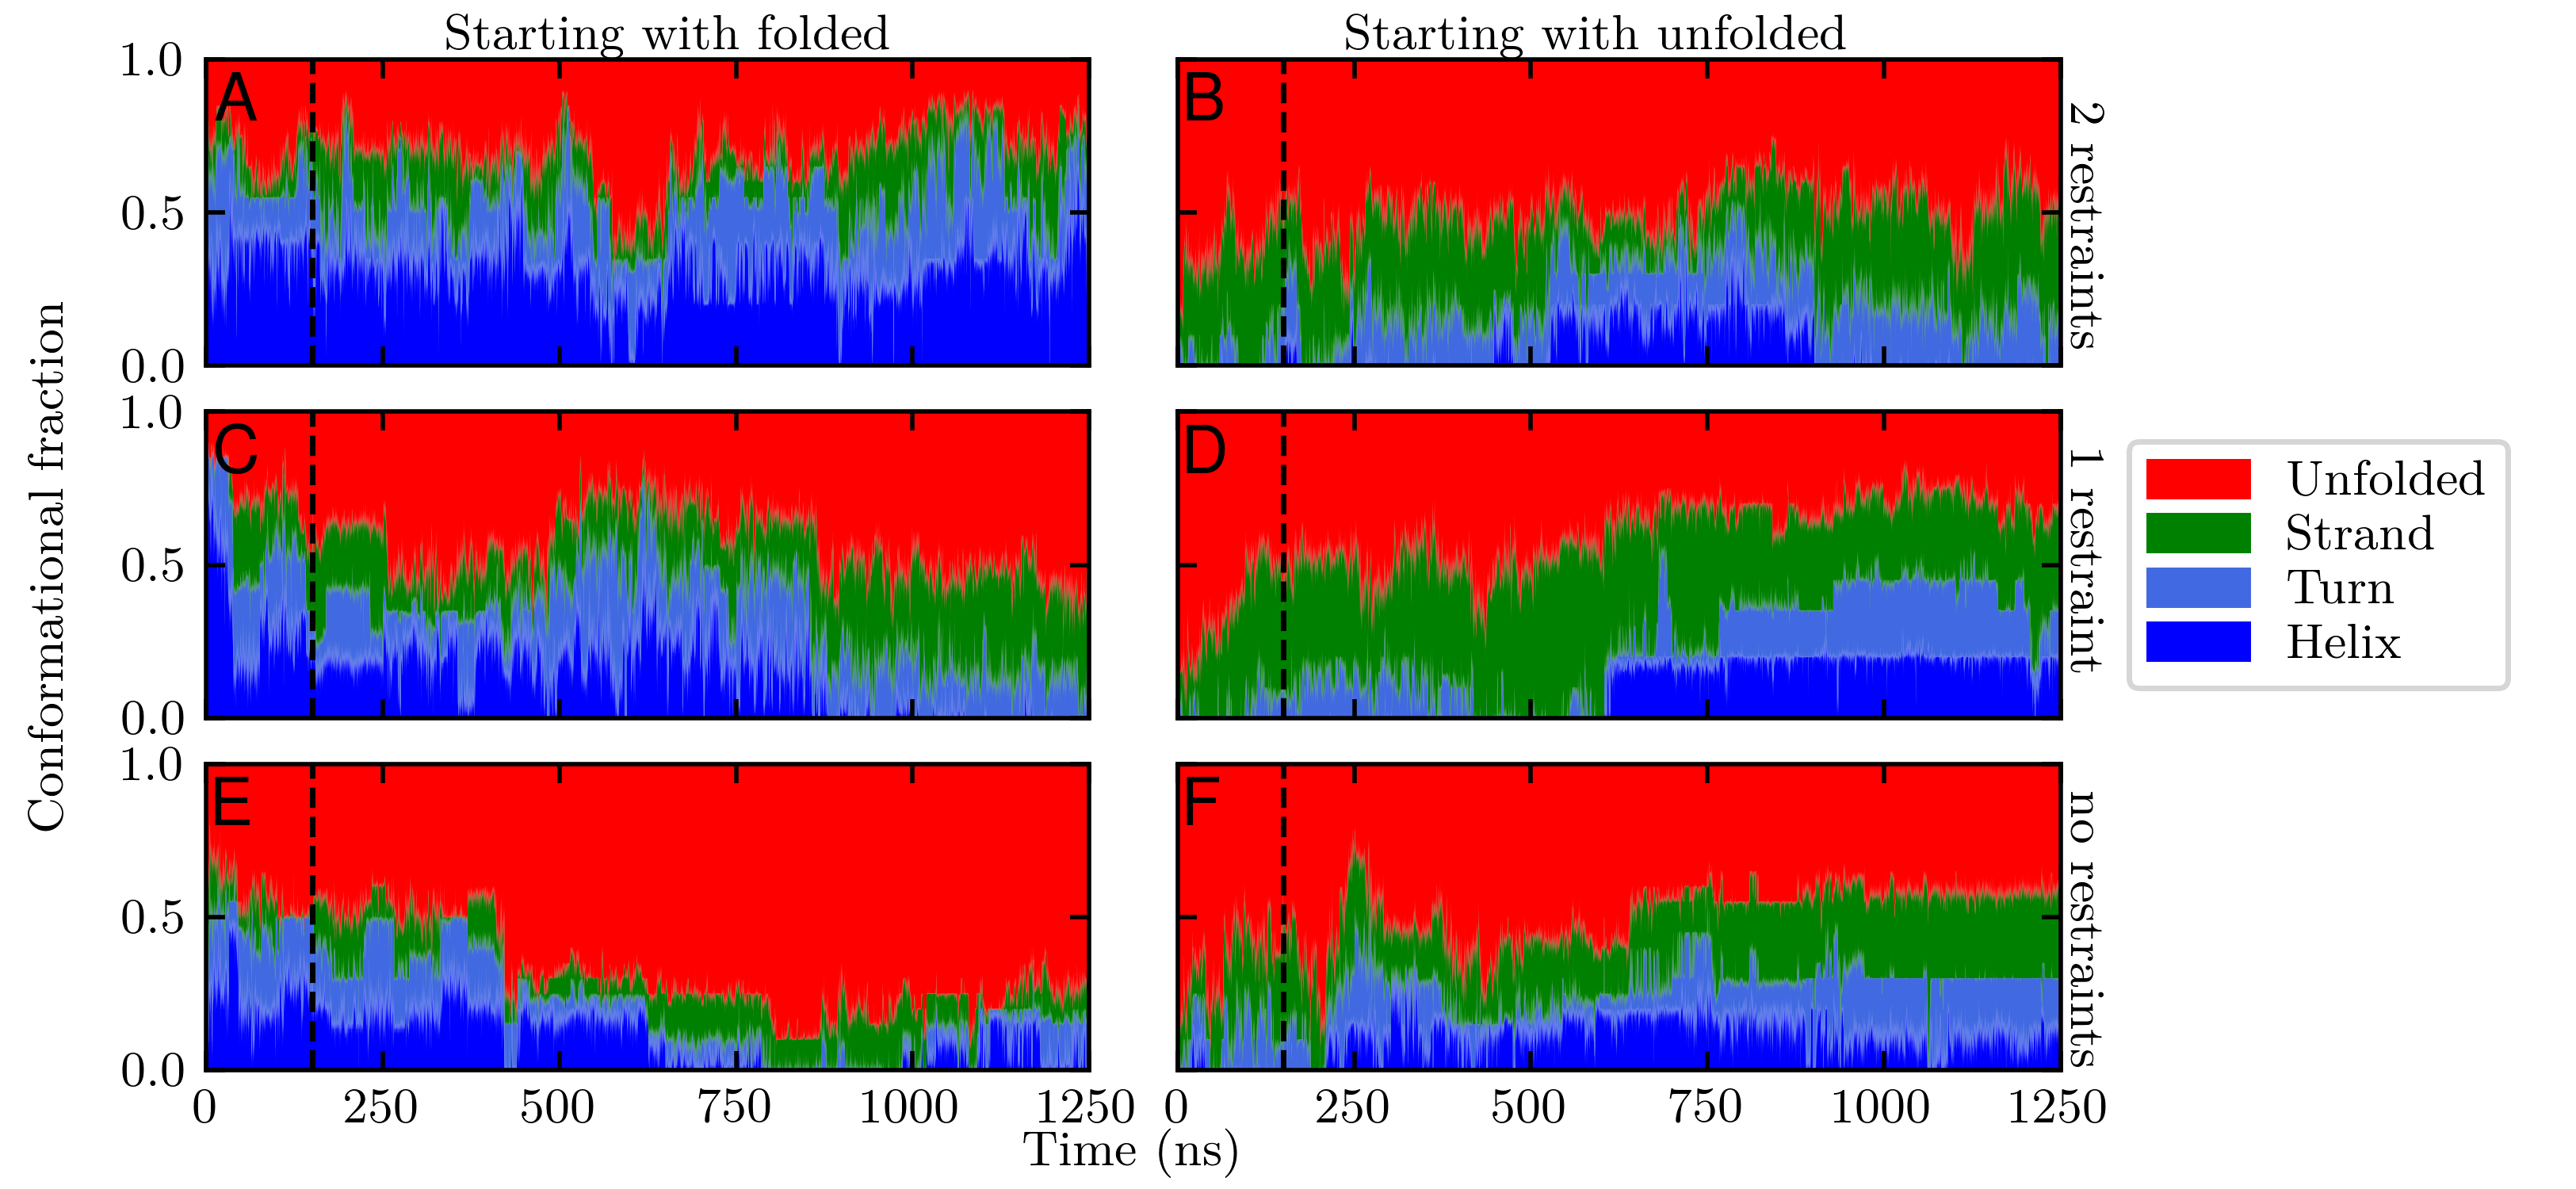
\includegraphics[width=6.0in]{figures-helix/disordered_helicity.png}
    \caption{
        Stacked conformational fractions of \pep{} on the surface of a \emph{disordered} SAM, with none, one, or two harmonic restraints between \pep{} and the SAM. 
        A, C, E: \pep{} began the simulation in an \textalpha{}-helical conformation. 
        B, D, F: \pep{} began the simulation unfolded. 
        A, B: \pep{} was harmonically restrained to the SAM at both glycine residues. 
        C, D: \pep{} was harmonically restrained to the SAM at only one of the glycine residues. 
        E, F: \pep{} was unrestrained on the SAM. 
        The data after this mark was averaged and is presented in Table \ref{tbl:helix-disorder}. 
    }
    \label{fig:helix-disorder}
\end{figure}

\begin{table}
    \caption{Average conformational fractions from simulations of \pep{} on the surface of a \emph{disordered} SAM in which either none, one, or both of the glycine residues in the peptide are harmonically restrained to the SAM.}
    \begin{center}
     \resizebox{6.0in}{!}{
     \begin{tabular}{c|cccc|cccc}
     \toprule
         Number of  & \multicolumn{4}{c}{From folded} & \multicolumn{4}{c}{From unfolded} \\
         harmonic restraints & Helix & Turn & Strand & Unfolded & Helix & Turn & Strand & Unfolded \\
     \midrule
         2 & 0.322 & 0.218 & 0.159 & 0.302 & 0.052 & 0.156 & 0.291 & 0.501 \\
         1 & 0.140 & 0.188 & 0.230 & 0.442 & 0.110 & 0.134 & 0.368 & 0.388 \\
         0 & 0.103 & 0.091 & 0.116 & 0.689 & 0.125 & 0.145 & 0.239 & 0.490 \\
     \bottomrule
     \end{tabular}
    }
    \end{center}
    \label{tbl:helix-disorder}
\end{table}

For the case of the simulations that started from a folded conformation where the peptide was bound by a single restraint or not bound to the SAM, the peptide rapidly unfolded on the disordered SAM (Figures \ref{fig:helix-disorder}C and \ref{fig:helix-disorder}E). 
In both cases, leucine residues were observed to move to divots in the disordered SAM surface (see Figure \ref{fig:helix-disordered_sam}B), presumably to maximize hydrophobic interactions with the decanethiol molecules. 
This movement often broke hydrogen bonds in the peptide backbone, destabilizing the helix. 
When these simulations were started from an unfolded configuration, the peptide did not fold over the course of the simulation (Figures \ref{fig:helix-disorder}D and \ref{fig:helix-disorder}F). 
None of the simulations on the disordered SAM had average conformational fractions consistent with the simulations of \pep{} on an ordered SAM, with exception of the simulation that started with a folded conformation and both glycine residues bound. 
All had significantly lower helix (0.140 or less) and turn character (0.188 or less), and higher unfolded character (0.388 or greater) than the simulations on the ordered SAM. 
In order to investigate the underlying reasons for these conformational differences, we calculated the free energy surfaces of \pep{} on the ordered SAM and \pep{} on the disordered SAM from the combined ensembles of structures. 
The ensemble of structures for each of these surfaces were constructed using all frames from the simulations with either one restraint or no restraints. 
The simulations with two restraints were excluded because of the convergence issues discussed above. 
The free energy surface of \pep{} on the ordered SAM is shown in Figure \ref{fig:helix-free_order}A. 
There is a distinct minimum free energy of -23.1 kJ mol$^{-1}$ with low $R_g$ and low backbone RMSD to the \textalpha{}-helical conformation. 
By contrast, the free energy surface on the disordered SAM (shown in Figure \ref{fig:helix-free_order}B) contains a weaker minimum ($\Delta G = -20.1$ kJ mol$^{-1}$) with slightly higher RMSD and higher $R_g$, indicative of destabilization of the compact, helical conformation on the SAM. 
Importantly, while the free energy minimum of \pep{} on the ordered SAM was distinct, the free energy profile of \pep{} on the disordered SAM was more diffuse and the minima less apparent. 
From these results, we hypothesize that the molecular-level order of the SAM surface is a driving force in the folding of the peptide. 
Our hypothesis is consistent with recent work by Dallin et al. that demonstrated that the apparent hydrophobicity of a SAM surface decreases with more disorder \cite{Dallin2019}.   
Since \pep{} was designed to fold at a polar/apolar interface\cite{DeGrado1985} and hydrophobic surfaces can stabilize helices\cite{Levine2016}, a decrease in hydrophobicity of the SAM surface likely decreases the entropic gain of the hydrophobic interactions of the leucine residues with the SAM surface. 
The peptide must therefore distort from a stable helical secondary structure to achieve strong hydrophobic interactions between the leucines and the SAM decanethiol. 
This thereby increases the free energy of the folding process, resulting in the larger $\Delta G$ of the folded conformation observed in Figure \ref{fig:helix-free_order}. 
Similar results have been reported for a shorter version of this peptide by Sprenger and Pfaendtner\cite{Sprenger2016}. 
We are currently investigating the dependence of the helical character of \pep{} on the extent of disorder of the SAM surface with additional simulations and experiments.  

\begin{figure}
    \center
    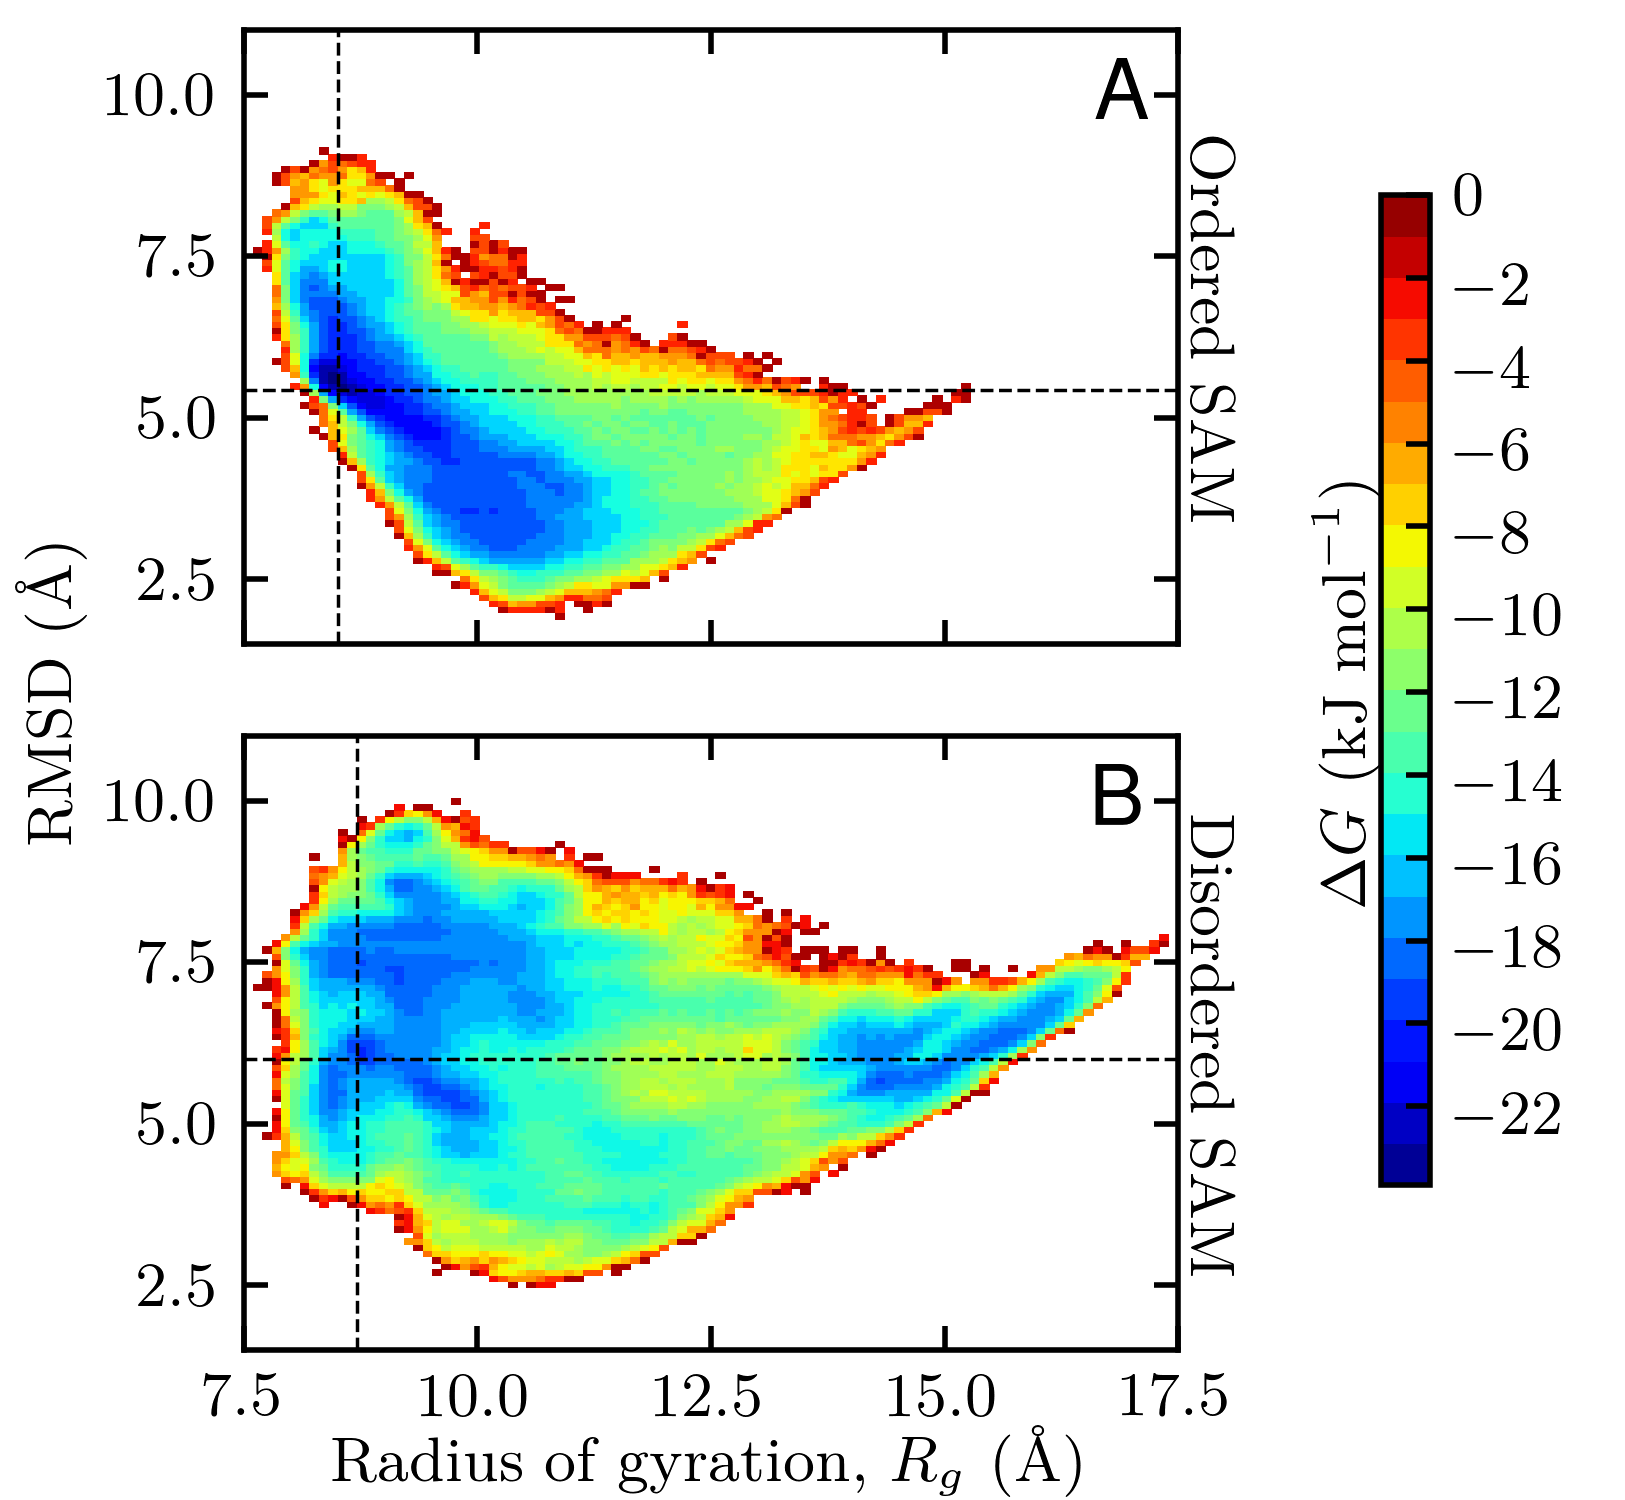
\includegraphics[width=3.25in]{figures-helix/comparison_free_energy_plots.png}
    \caption{
        Free energy surfaces of the combined ensembles of structures of \pep{} on the ordered SAM (A) and of \pep{} on the disordered SAM (B). 
        The combined ensembles exclude the trajectories with two restraints and structures prior to the equilibration time, as discussed in the main text. 
        On the $x$-axis is the radius of gyration of the protein. 
        On the $y$-axis is the backbone RMSD away from a perfectly folded \textalpha{}-helix. 
        The intersection of the dashed lines is the global minimum for each surface. 
    }
    \label{fig:helix-free_order}
\end{figure}

%%%%%%%%%%%%%%%%%%%%%%%%%%%%%%%%%%%%%%%%%%%%%%%%%%%%%%%%%%%%%%%%
%%%%%%%%%%%%%%%%%%%%%%%%%%%%%%%%%%%%%%%%%%%%%%%%%%%%%%%%%%%%%%%%
\section{Conclusion}\index{helix-conclusion}
%%%%%%%%%%%%%%%%%%%%%%%%%%%%%%%%%%%%%%%%%%%%%%%%%%%%%%%%%%%%%%%%
%%%%%%%%%%%%%%%%%%%%%%%%%%%%%%%%%%%%%%%%%%%%%%%%%%%%%%%%%%%%%%%%

The accuracy and applicability of canonical force fields such as OPLS-AA to complex environments is not automatic since these force fields were parameterized against structural information in the PDB, which is vastly overrepresented by compact globular proteins in dilute solution. 
However, using a set of 6 simulations of 1.25 \textmu{}s each of the charged peptide \pep{}, we demonstrated that widely available resources and the OPLS-AA force field were sufficiently accurate to describe the conformational change of our peptide induced by a binary solvent (\tbawat{}) and a SAM surface. 
We have demonstrated that while our simulations overestimated the amount of \textbeta{}-sheet character of the peptide in water, the conformational fractions from the simulations were quantitatively accurate to secondary structure estimates obtained from deconvoluting the experimental CD spectra. 
We further computed the CD spectra from the MD simulations, showing qualitative agreement with the experimental spectra. 
After demonstrating the accuracy of the simulations, we presented 10 additional 1.25 \textmu{}s simulations of \pep{} on the SAM surface under a variety of conditions. 
While we are unable to verify these final simulations with existing experimental data, they suggest two specific hypotheses about factors that may be important in peptide structure at a surface: 
1) the peptide must fold before the second covalent attachment to the surface; and 
2) the order of the SAM surface is a significant driving force to the folding process. 
These two hypotheses are currently being tested in our laboratory. 
While these results should not be extended arbitrarily to other systems, the ability to simulate accurate structural changes of biomolecules near surfaces or in otherwise complex environments has far reaching implications on plaque diseases, such as Alzheimer's disease, and can greatly aid in the incorporation of biomolecules onto surfaces for use in biosensors and catalytic devices. 





\chapter{Orthogonal Electric Field Measurements near the Green Fluorescent Protein Fluorophore through Stark Effect Spectroscopy and \pKa{} Shifts Provide a Unique Benchmark for Electrostatics Models} \label{gfp-pKa}

%Measurement of the magnitude, direction, and functional importance of electric fields in biomolecules has been a longstanding experimental challenge. 
%\pKa{} shifts of titratable residues have been the most widely implemented measurements of the local electrostatic environment around the labile proton, and experimental data sets of \pKa{} shifts in a variety of systems have been used to test and refine computational prediction capabilities of protein electrostatic fields. 
%A more direct and increasingly popular technique to measure electric fields in proteins is Stark effect spectroscopy, where the change in absorption energy of a chromophore relative to a reference state is related to the change in electric field felt by the chromophore. While there are merits to both of these methods and they are both reporters of local electrostatic environment, they are fundamentally different measurements, and to our knowledge there has been no direct comparison of these two approaches in a single protein. 
%We have recently demonstrated that green fluorescent protein (GFP) is an ideal model system for measuring changes in electric fields in a protein interior caused by amino acid mutations using both electronic and vibrational Stark effect chromophores. 
%Here we report the changes in \pKa{} of the GFP fluorophore in response to the same mutations and show that they are in excellent agreement with Stark effect measurements. 
%This agreement in the results of orthogonal experiments reinforces our confidence in the experimental results of both Stark effect and \pKa{} measurements, and provides an excellent target dataset to benchmark diverse protein electrostatics calculations. 
%We used this experimental dataset to test the \pKa{} prediction ability of the Adaptive Poisson-Boltzmann Solver (APBS) and found that a simple continuum dielectric model of the GFP interior is insufficient to accurately capture the measured \pKa{} and Stark effect shifts . 
%We discuss some of the limitations of this continuum-based model in this system and offer this experimentally self-consistent dataset as a target benchmark for electrostatics models, which could allow for a more rigorous test of \pKa{} prediction techniques due to the unique environment of the water-filled GFP barrel compared to traditional globular proteins.

%%%%%%%%%%%%%%%%%%%%%%%%%%%%%%%%%%%%%%%%%%%%%%%%%%%%%%%%%%%%%%%%
%%%%%%%%%%%%%%%%%%%%%%%%%%%%%%%%%%%%%%%%%%%%%%%%%%%%%%%%%%%%%%%%
\section{Publication note} \label{pKa-pub-note}
%%%%%%%%%%%%%%%%%%%%%%%%%%%%%%%%%%%%%%%%%%%%%%%%%%%%%%%%%%%%%%%%
%%%%%%%%%%%%%%%%%%%%%%%%%%%%%%%%%%%%%%%%%%%%%%%%%%%%%%%%%%%%%%%%

Portions of this chapter are adapted from the following publication: 

\noindent Joshua D. Slocum, Jeremy T. First, Lauren J. Webb; Orthogonal Electric Field Measurements near the Green Fluorescent Protein Fluorophore through Stark Effect Spectroscopy and \pKa{} Shifts Provide a Unique Benchmark for Electrostatics Models. emph{Journal of Physical Chemistry B}. \textbf{2017}, \emph{121}, 6799-6812.

JTF performed all calculations. 
All code, force field parameters, structures, and other starting files used for the simulation, analysis, processing of data, and figure generation can be accessed at:
\url{https://github.com/jeremyfirst22/GFP_pKa}. 
JDS performed all experiments. The experimental methods are ommited from this Chapter, but they may be found in the publication. 

%%%%%%%%%%%%%%%%%%%%%%%%%%%%%%%%%%%%%%%%%%%%%%%%%%%%%%%%%%%%%%%%
%%%%%%%%%%%%%%%%%%%%%%%%%%%%%%%%%%%%%%%%%%%%%%%%%%%%%%%%%%%%%%%%
\section{Introduction} \label{pKa-intro}
%%%%%%%%%%%%%%%%%%%%%%%%%%%%%%%%%%%%%%%%%%%%%%%%%%%%%%%%%%%%%%%%
%%%%%%%%%%%%%%%%%%%%%%%%%%%%%%%%%%%%%%%%%%%%%%%%%%%%%%%%%%%%%%%%

Electrostatic fields have long been recognized as a key driving force behind all protein functions, including folding, stability, noncovalent interactions with small molecules or large biological macromolecules, catalysis, and other reactivity \cite{Hayes1976, Warshel1978, Honig1995, Gunner1996, Warshel1998}.
Because electric fields generated by the arrangement of partial charges in the structure of a protein are long-range, the electrostatic environment of a protein can be quite complex at the molecular length scale. 
This makes characterizing the magnitude and effect of electric fields in biological molecules a difficult task from both experimental and computational perspectives. 
The most widely implemented experimental technique used to measure electrostatic effects in proteins has been quantifying the perturbation of \pKa{} values of titratable amino acid side chains compared to their values in aqueous buffer \cite{Forsyth2002, Langsetmo1991, Isom2010, Bradbury1966, Markley1975}.
The three-dimensional arrangement and connectivity of partially charged atoms near the titratable residue creates an electrostatic environment that strongly influences the relative stability of charged versus neutral side chains. 
Because of this, the measurement of the equilibrium between these two states is often thought to be a good reporter of the local electrostatic environment around the amino acid. 
\pKa{} values can be measured straightforwardly by recording the pH-dependence of a signal that changes with protonation state; this is commonly done by measuring chemical shifts of labile $^1$H or nearby $^{13}$C atoms by NMR \cite{Markley1975}. 
Experiments like these have led to the estimation of dielectric constants of globular proteins \cite{Dwyer2000, Chimenti2011}, helped rationalize the catalytic mechanisms of enzymes \cite{Inoue1992, Davoodi1995, McIntosh1996}, and have led to an understanding of how charged amino acids can be accommodated in the interior of proteins \cite{Isom2010, Chimenti2011, Isom2008}.

While these \pKa{} values are excellent reporters of the overall electrostatic environment around the titratable residue, it is typically very difficult to rationalize which specific interactions contribute most significantly to the observed equilibrium. 
For instance, lysine, whose side chain \pKa{} is $\sim$10.5 in water, often titrates with a significantly lower \pKa{} when buried in the non-polar interior of a protein. 
This is due to the overall energetic favorability of the non-polar protein environment to contain the neutral form of lysine rather than the charged form. 
However, without further experimental and theoretical investigations, the perturbed \pKa{} values of lysine residues do not offer significant information with molecular level detail of the specific electrostatic interactions that cause the \pKa{} shift.  

Because of the sensitivity of \pKa{} values of titratable amino acid side chains to the overall electrostatic environment around the amino acid, one significant aspect of accurate \pKa{} measurements in proteins is their usefulness as benchmarks for electrostatics models \cite{Gibas1996, Antosiewicz1996, Fogolari2002, Li2005, Olsson2011, Witham2011, Meyer2015, Mehler1999}.
However, this sensitivity can also be viewed as a drawback for modeling, because of the necessity to accurately model long range interactions in a complex protein environment. 
Many attempts have been made to predict the \pKa{} values of different amino acids in proteins to validate electrostatics models with levels of theory ranging from fully atomistic quantum mechanics, to mixed quantum mechanics, to continuum electrostatics \cite{Gibas1996, Antosiewicz1996, Schutz2001, Warshel2006, Nielsen2011}.
However, because of the complexity of electrostatic environments in proteins, the accurate modeling of electrostatic effects often requires excessive computational cost or a vast oversimplification of the relevant physics. 
Most electrostatics models can adequately reproduce the \pKa{} values of solvent exposed side chains that experience negligible shifts in \pKa{} relative to their values in water, but the successful calculation of perturbed \pKa{} values of buried residues, which have been observed to shift by as much as 5 \pKa{} units, is much more difficult \cite{Schutz2001, Simonson2001}.
This requires an accurate and detailed treatment of the complex environment of a protein interior, including dynamic fluctuationsequilibrium sampling \cite{Schutz2001, Nielsen2011, Warshel2011, Alexov2011, Li2013}.

Many current strategies for calculating \pKa{} shifts in proteins involve the use of a thermodynamic cycle to calculate the change in free energy when the titratable residue in question is transferred from water to the protein environment \cite{Fogolari2002, Gorham2011, Getahun2003}.
The strategy taken to accurately calculate these electrostatic free energies is where many common models deviate, although most are based on continuum electrostatics models such as the Poisson-Boltzmann (PB) equation. 
Algorithms to generate distributions of charge states and starting structures for the energy calculations generally increase the agreement with experiment, which suggests that protein fluctuations and charge state coupling are important \cite{Witham2011, Meyer2015}.
However, regardless of the approach, electrostatics models still do a poor job at reproducing \pKa{} shifts of buried residues. 
Indeed, in a recent collaboration between many researchers, blind predictions of the \pKa{} values of 25 lysine residues in the interior of \emph{Staphylococcal} nuclease were made using a variety of different strategies, each meeting only limited success \cite{Nielsen2011, Alexov2011}.
Most of the techniques reported in the study were based on continuum electrostatics models that differed in their approach to sampling conformational and charge space of the protein atoms. 
While many of the approaches could accurately predict the direction of the \pKa{} shifts relative to the value in water, often the magnitude of the \pKa{} shifts were off by several \pKa{} units. 
Because many of the current strategies depend on an accurate calculation of the total electrostatic energy of the protein, which is sensitive to many factors, such as protein conformation, dipole moments, and polarizability, it is often difficult to assess which aspects of a given model contribute to both the agreement and disagreement between experiment and calculation. 
In this work, we provide experimental measurements of specific electrostatic effects, namely site-specific electric fields in the interior of a protein, to complement \pKa{} measurements of a titratable residue in the same electrostatic environment with the goal of providing two orthogonal benchmarks for electrostatics models.

An increasingly popular technique to measure local electrostatic fields in proteins is Stark effect spectroscopy \cite{Fafarman2010, Fried2014, Stafford2012}.
In this technique, a probe transition with a characteristic difference dipole moment, $\Delta \vec{\mu}$, is inserted into the protein and its absorption energy is measured. 
Changes in the energy, $\Delta E$, due to a chemical perturbation such as amino acid mutation are related to the change in electric field, $\Delta\vec{F}$, caused by the perturbation through equation \ref{eq:stark}: 
\begin{equation}
\Delta E = - \Delta\vec{\mu}\cdot\Delta\vec{F}
\label{eq:stark}
\end{equation}
Equation \ref{eq:stark} is the exact form of the linear Stark effect, where higher order non-linear terms are assumed to be negligible. 
Many vibrational chromophores have been shown to adhere to this simplified model, and have been used successfully to measure electrostatic effects at enzyme active sites \cite{Webb2008, Fafarman2012}, protein-protein interfaces \cite{Stafford2010, Walker2014}, and in the interior of model membranes \cite{Hu2011, Shrestha2015}.
Of particular interest to us is the nitrile stretching oscillation Stark probe, because it absorbs in a relatively clear region of the infrared spectrum ($\sim$2100-2250 \si{\wn}), has a reasonable oscillator strength ($\epsilon \approx 200$ \si{M\tothe{-1} \wn}), and is strongly sensitive to changes in electric field ($\Delta\vec{\mu} \approx 1$ \si{\wn/(MV/cm))} \cite{Webb2008}.
Additionally, for the nitrile stretch, $\Delta\vec{\mu}$ lies along the C---N bond axis, meaning that the change in energy from Equation \ref{eq:stark} is a direct reporter of the changes in electric field in the direction of the nitrile bond vector. 
Because of this, when coupled with information about the orientation of the Stark effect probe from crystal structures or molecular dynamics (MD) simulations, Stark effect measurements can provide information about both the magnitude and direction of relative electric fields in a complex protein environment, which is not possible from \pKa{} measurements of titratable residues alone. 

Measurements of the direction and magnitude of electric field changes in proteins could provide a convenient complement to \pKa{} measurements of titratable residues for researchers who wish to benchmark electrostatics models.  
In principle, because \pKa{} values are determined in part by electrostatic interactions, and site-specific electric fields represent the force at a particular location due to the surrounding electrostatic environment, these two types of measurements might be expected to respond similarly to the same perturbations. 
However, they represent an orthogonal set of measurements which can be used to describe electrostatic effects in fundamentally different ways, and to our knowledge, there has been no direct comparison of \pKa{} and Stark effect measurements in the same system. 
It is the goal of this work to compare \pKa{} shifts to spectroscopically measured electric field changes, caused by the same perturbations in a protein.

Recently, we reported measurements of electric fields in superfolder green fluorescent protein (GFP), inferred from Stark effect shifts of biosynthetically incorporated nitrile probes and from the GFP fluorophore, in response to a series of amino acid mutations \cite{Slocum2016}.
We observed an agreement between these two types of Stark effect probes, allowing us to interpret the spectroscopic responses of these probes in terms of electric fields. 
Because the GFP fluorophore, shown in Figure \ref{fig:system}, can be protonated or deprotonated at physiological pH, it provides a convenient \pKa{} probe in the vicinity of the nitrile vibrational Stark effect (VSE) probes. 
Additionally, the embedded fluorophore in superfolder GFP is formed from the residues T65-Y66-G67 (hereafter TYG), which has been shown to obey the linear Stark effect\cite{Bublitz1998} (Equation \ref{eq:stark}) and is more sensitive to pH changes than the wild type fluorophore (S65-Y66-G67) due to reduced coupling between Y66 and the surrounding titratable residues \cite{Oltrogge2012, Brejc1997}.

\begin{figure}
    \center
    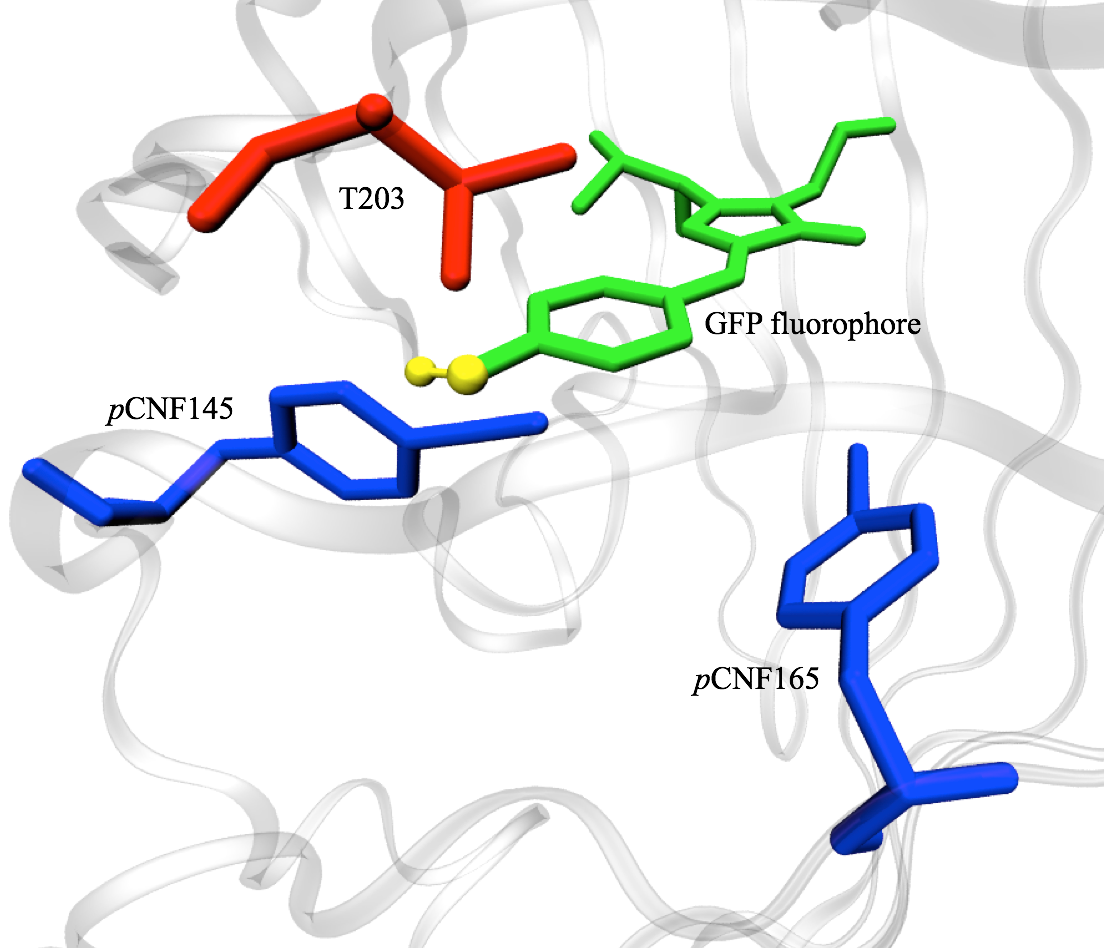
\includegraphics[width=\single]{figures-gfp-pKa/system.png}
    \caption[Probe and T203 locations near the GFP fluorophore]{
        A close-up view of the interior of GFP (gray ribbon) modeled from crystal structure 2b3p. 
        The GFP fluorophore is shown in green with the titratable --OH shown in yellow. 
        \pCNF{} 145 and 165 are shown in blue, and position 203 is shown in red.
    }
    \label{fig:system}
\end{figure}

Here we report the \pKa{} values of this fluorophore, estimated from the pH-dependent absorption spectra of the GFP fluorophore, as a function of the same mutations. 
To do this, we inserted the unnatural amino acid, \emph{p}-cyanophenylalanine (\pCNF{}), at either position 145 or 165, which are both near the GFP fluorophore, and made a series of mutations to position 203 (Figure \ref{fig:system}). 
We then measured the effect of these mutations on the electrostatic environment in the vicinity of the flourophore both through VSE spectroscopy of the two nitrile probes and \pKa{} and Stark effect measurements of the flourophore itself. 
Our results show that the \pKa{} shifts in response to the amino acid mutations are linearly correlated with the site specific electric field changes, measured from either the vibrational or electronic Stark effect probes. 
This agreement provides confidence that Stark effect shifts and \pKa{} shifts respond similarly to the same electrostatic perturbations. 
This trend was not observed when histidine or cysteine were at position 203, which we hypothesize was due to (1) differences in the hydrogen bonding network around the fluorophore caused by histidine and cysteine at position 203; or (2) the interference of the fluorophore titration by the simultaneous titration of histidine or cysteine at position 203. 
Because of the potential for this experimentally self-consistent model system to be a benchmark for electrostatics models, we also attempted to calculate the \pKa{} values using APBS and MD simulations.
However, even when we included 50 \si{\ns} of protein dynamics, APBS was unable to accurately reproduce the experimental \pKa{} values. 
We predict that a more advanced calculation than one based on a continuum electrostatic treatment of the interior of GFP is likely necessary to accurately predict \pKa{} values inside the unique \textbeta{}-barrel protein. 
All together, this model system contains a VSE probe, an electronic Stark effect probe, and a \pKa{} probe that all respond similarly to perturbations at position 203. 
In addition to providing confidence in our ability to measure electrostatic effects experimentally, we also believe that these experimental data are an excellent target data set for benchmarking a variety of computational electrostatics models.

%%%%%%%%%%%%%%%%%%%%%%%%%%%%%%%%%%%%%%%%%%%%%%%%%%%%%%%%%%%%%%%%
%%%%%%%%%%%%%%%%%%%%%%%%%%%%%%%%%%%%%%%%%%%%%%%%%%%%%%%%%%%%%%%%
\section{Experimental methods} \label{pKa-methods}
%%%%%%%%%%%%%%%%%%%%%%%%%%%%%%%%%%%%%%%%%%%%%%%%%%%%%%%%%%%%%%%%
%%%%%%%%%%%%%%%%%%%%%%%%%%%%%%%%%%%%%%%%%%%%%%%%%%%%%%%%%%%%%%%%

%\subsection{Protein Expression and Purification}
%
%A pBAD vector containing the gene for His6-tagged super folder GFP and a pDULE vector coding for an orthogonal tRNA/synthetase pair optimized for \pCNF{} were a generous gift from the Mehl lab \cite{Miyake-Stoner2010}.
%Mutations to the pBAD vector at amino acid positions 145, 165, or 203 were made using a Quik-Change II site directed mutagenisis kit from Agilent.
%To make each nitrile-containing GFP mutant, DH10\textbeta{} cells were co-transformed with both the pBAD vector (containing the \emph{amber} stop codon at amino acid position 145 or 165, and the proper codon for amino acid 203) and the pDULE vector. 
%These co-transformed cells were grown in an autoinduction media as described elsewhere \cite{Hammill2007}.
%Mutants without a nitrile probe were purified from DH10\textbeta{} cells expressing only the pBAD vector. 
%In both cases, the His$_6$-tagged mutants were purified as outlined previously by immobilized metal affinity chromatography, the tags cleaved and separated, and the purified protein used immediately or stored at $-80$ \si{\celsius} \cite{Slocum2016}. 
%
%\subsection{pH Titrations}
%
%Purified GFP mutants were buffer exchanged into a master buffer containing 50 \si{mM} phosphate, 50 mM citrate, and 100 mM NaCl at pH 7.5, and the buffer-exchanged protein was concentrated to $\sim$1 mM using centrifugal filters. 
%UV-Vis absorption spectra of the GFP mutants were recorded from pH 5 to 10 on a Biotek Epoch 2 microplate reader between 250-600 nm. 
%The plates were prepared by mixing 2 $\mu$L of the concentrated protein with 300 $\mu$L of the master buffer (adjusted to the desired pH with acid or base) into the wells of a UV-transparent 96-well plate. 
%For each mutant, at least three pH titrations were carried out.
%
%\subsection{UV-Vis and FTIR Spectroscopy}
%
%For all absorption spectroscopy measurement besides the pH titrations, purified GFP mutants were buffer exchanged into PBS at pH 7.4. 
%UV-Vis absorption spectra were collected in a 1 cm quartz cuvette using a Cary 5000 spectrometer with 0.1 nm resolution. 
%FTIR absorption spectra of the nitrile-labeled mutants were collected using a Bruker Vertex 70. 
%Protein samples concentrated to 1-2 mM were injected between two sapphire windows separated by 125 $\mu$m Teflon spacers. 
%Spectra were collected by averaging 250 scans with 0.5 \si{\wn} resolution. 
%After subtracting a background spectrum of PBS, the spectra were baseline-corrected and fit to Gaussian functions using an in-house program that has been described previously \cite{Ragain2012}.
%All spectra were measured at least three times.   

\subsection{Molecular Dynamics Simulations}

A template protein structure was modeled by homology from the 2b3p crystal structure\cite{Pedelacq2006} using the MODELLER software package \cite{Marti-Renom2000}.
From this template, the 6 different mutations were made to position 203 using the mutagenesis wizard tool in PyMol \cite{DeLano2002}.
For each of these 7 protein systems, the residue at position 145 or 165 was independently mutated to \pCNF{} and minimized using the Avogadro molecular editing package \cite{Hanwell2012}. 
Special care was taken with the titration state of Glu222, which was assigned a neutral state based on indirect crystallographic evidence of the fluorophore hydrogen bonding environment from Elsliger et al \cite{Elsliger1999}. 
Histidine residues at positions 25, 148 181, 199 and 217 were protonated at the N$_{\delta}$, and histidine residues at positions 77, 81, 139 and 169 was protonated at the N$_{\varepsilon}$, following the simulation protocol by Nifos\'i et al \cite{Nifosi2003}.
The histidine at position 231 is not present in either of the two studies cited, and was protonated at the N$_{\varepsilon}$ as determined to be most favorable by pdb2gmx. 
Finally, each of these 21 structures was edited to reflect the two different protonation states of the internal GFP chromophore, resulting in 42 different protein systems for the start of molecular dynamics (MD) simulations. 

Parameters for the protonated and deprotonated chromophore were kindly provided by Riccardo Nifos\'i \cite{Nifosi2003}.
The RESP fitting procedure was used to fit point charges to the electrostatic potential calculated using GAMESS \cite{Bayly1993}.
Bonded parameters for the nitrile group were taken from those previously developed by our group for cyanocysteine \cite{Ragain2012}.
All other bonded parameters were taken by analogy from tyrosine. 
All further minimizations and MD simulations were performed using the Gromacs 5.0.4 molecular dynamics software package \cite{VanDerSpoel2005, Abraham2015} and the Amber03 force field (ffAmber03) \cite{Duan2003, Sorin2005}.
Each of the 42 protein systems was energy minimized in vacuum using steepest descent, and solvated in an 80 \si{\angstrom} dodecahedron box of TIP3P water to ensure that the protein would not interact with itself through the periodic boundary conditions \cite{Jorgensen1983}.
All resulting systems had a net negative charge, which was neutralized with the addition of 5-7 sodium ions, depending on the protein system. 
These solvated systems were energy minimized with heavy atom restraints on the protein, and then were subjected to 100 ps of simulation at constant pressure and 50 ps of simulation at constant volume to equilibrate the solvent, again using heavy atom restraints. 
Production MD was run on each protein system for 50 \si{\ns}, using a time step of 2 fs and stochastic integrator. 
Particle Mesh Ewald electrostatics was implemented with a coulomb cut-off of 8 \si{\angstrom} \cite{Cheatham1995}.
Van der Waals (VDW) interactions were cut off at 8 \si{\angstrom}. 
Snapshots were recorded every 4 ps during the simulations.  

\subsection{Electrostatic Free Energy Calculations in APBS}

At every 500 ps of each simulation, molecular structure, including a 5 \si{\angstrom} sphere of explicit waters as discussed below, was extracted using the Gromacs utilities select and trjconv. 
Charges and VDW radii were assigned to the molecular structures using the pdb2pqr utility provided with the APBS v1.4 software package \cite{Dolinsky2007}.
The GFP chromophore and \pCNF{} charges were taken in accordance with their simulation point charges, and VDW radii were assigned by analogy to other atom types.

To assess the free energy of protein-solvation, three electrostatic free energy calculations were performed using APBS on the protein-solvent structure, the protein-solvent structure with charges on the chromophore removed, and an isolated chromophore structure. 
In each of these calculations, the same grid spacing was used in accordance with the default pdb2pqr suggestion for a system of this size. 
The solvent region was assigned a dielectric constant of 78.54 and the protein region was assigned a dielectric constant of 6. 
For free energy calculations on the crystal structures, the protein region and any crystallized water molecules were assigned a dielectric constant of 20 instead as the conformational flexibility of the protein was not explicitly simulated.

%%%%%%%%%%%%%%%%%%%%%%%%%%%%%%%%%%%%%%%%%%%%%%%%%%%%%%%%%%%%%%%%
%%%%%%%%%%%%%%%%%%%%%%%%%%%%%%%%%%%%%%%%%%%%%%%%%%%%%%%%%%%%%%%%
\section{Results and Discussion} \label{pKa-results}
%%%%%%%%%%%%%%%%%%%%%%%%%%%%%%%%%%%%%%%%%%%%%%%%%%%%%%%%%%%%%%%%
%%%%%%%%%%%%%%%%%%%%%%%%%%%%%%%%%%%%%%%%%%%%%%%%%%%%%%%%%%%%%%%%

\subsection{\pKa{} Measurements}

To compare the ability of \pKa{} shifts and Stark effect shifts to report on changes in electrostatic environment in a protein, we mutated the wild type T203 (where T represents the one letter code of threonine and 203 is the amino acid position in the primary sequence) of superfolder GFP to S, N, H, C, F, and Y and inserted a \pCNF{} residue at either position 145 or 165 (Figure \ref{fig:system}). 
To estimate the equilibrium between the neutral and ionized fluorophore, we measured the pH dependence of the visible absorption of the fluorophore over a range of pH 5-10.  
Figure \ref{fig:abs_titrations} shows the pH-dependent visible absorption spectra of a representative GFP mutant, S203 (Figure \ref{fig:abs_titrations}A), and the resulting titration curve (Figure \ref{fig:abs_titrations}B), from which the \pKa{} values were determined. 
As expected, the fluorophore population shifted from mostly protonated (A state) at low pH to mostly de-protonated (B state) at high pH.
The presence of a clean isosbestic point indicated that there were only two states participating in the equilibrium.
Plotting the maximum absorbance of both the A and the B states as a function of the solution pH resulted in two curves which could be fit to a single sigmoidal function and used to find the inflection point.
The curve fitting application of Matlab R2016a was used to fit all titration curves to a sigmoidal function of the form shown in Equation \ref{eq:sigmoid},
\begin{equation}
    \text{Abs}(\pH) = \frac{a}{b+e^{c\cdot\pH}}+d
    \label{eq:sigmoid}
\end{equation}
where Abs(pH) is the maximum absorbance of either the A or B state at a given pH, $a$ is the maximum value of Abs, $b$ defines the offset of the function from pH = 0, $c$ defines the pitch of the sigmoid, and $d$ is the minimum value of Abs \cite{Matlab2016}.
The inflection point of the resulting fit was taken to be the \pKa{} for that mutant.
With the exception of the few cases where the A state titration could not be fit (Y203, H203, and H203 with \pCNF{} 165), titrations of both the A and B states gave \pKa{} values that were within experimental error of each other, < 0.08 \pKa{} units.
In the cases where only one titration could be fit to a sigmoidal curve, the \pKa{} was estimated directly from that titration.
The fact that 39 of the 42 titrations could be well described by a single site titration model suggests that any coupling of the fluorophore titration to other nearby titratable residues was negligible. 

\begin{figure}
    \center
    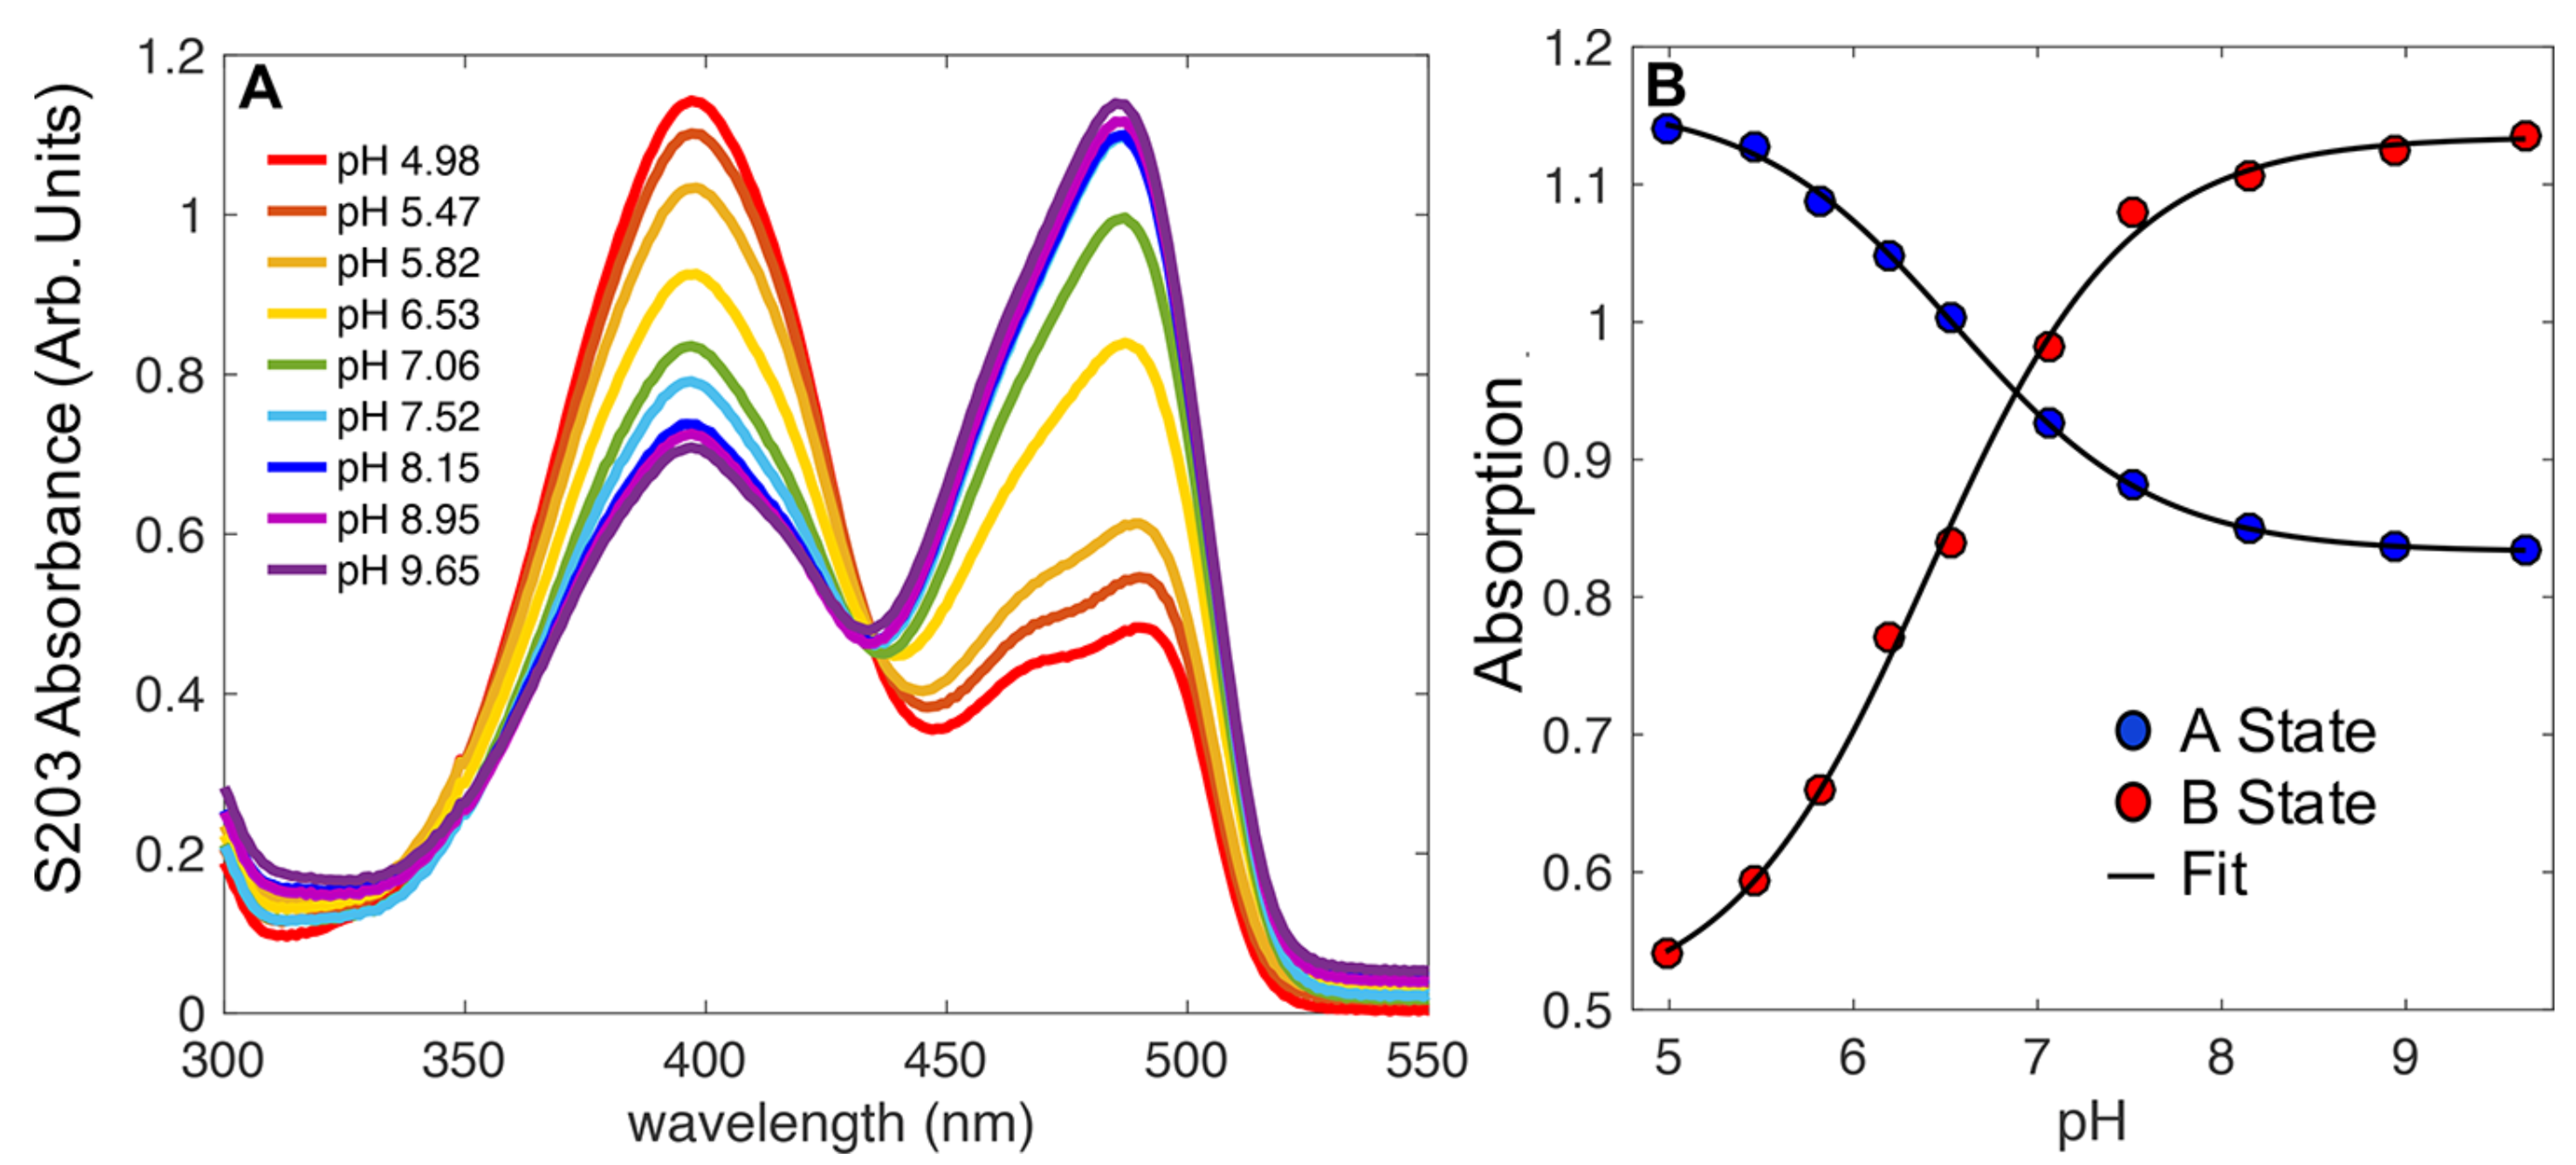
\includegraphics[width=\double]{figures-gfp-pKa/absorption_titrations.png}
    \caption[Representative titration of the GFP fluorophore]{
        A representative titration of the GFP fluorophore. 
        Panel A shows the visible absorption spectra of the fluorophore of S203 over a range of pH values given by the color code. 
        Panel B shows the maximum absorption of the A state (blue) and the B state (red) of the S203 spectra from panel A, plotted against the solution pH. 
        The solid lines are sigmoidal fits which are used to estimate the \pKa{}.
    }
    \label{fig:abs_titrations}
\end{figure}

Table \ref{tbl:pKas} shows the \pKa{} values obtained for all 21 of the mutant constructs.
Overall, we measured a range of \pKa{} values from 6.28-7.95, which is typical for GFP mutants containing the TYG fluorophore.
Previous studies have suggested that two dominating contributions to GFP fluorophore \pKa{} values are (1) specific hydrogen bonding to or from the fluorophore phenolate (or phenol), determined by the local hydrogen bonding network of water and protein residues around the fluorophore; and (2) aromatic interactions with the fluorophore from nearby side chains that tend to stabilize the neutral form of the fluorophore \cite{Elsliger1999, Wachter1998}.
Here, the measured \pKa{} values tended to increase as we placed aromatic residues at position 203, and the lowest \pKa{} values were measured for the small, polar residues at position 203.
This suggests that aromatic interactions between the fluorophore and Y and F at position 203 are responsible for the elevated \pKa{} values we have measured here, and that the hydrogen bonding environment around the fluorophore might play a larger role in the \pKa{} values for the other position 203 mutants. 

\begin{table}
    \caption[Experimental \pKa{} values of the GFP chromophore]{
        A Summary of the Measured \pKa{} Values for All GFP Mutants$^a$
    }
    \begin{center}
    \begin{tabular}{c|ccc}
        \toprule
        \rowcolor{lgray}
        position 203 & WT & \pCNF{} 145 & \pCNF{} 165 \\

        \cmidrule(r){1-1}\cmidrule(l){2-4}
        T$^b$ &   $ 6.70 \pm 0.07 $  &  $ 6.63 \pm 0.04 $ &  $ 7.17 \pm 0.03 $  \\
        F     &   $ 7.50 \pm 0.03 $  &  $ 7.20 \pm 0.04 $ &  $ 7.51 \pm 0.05 $  \\
        C     &   $ 6.85 \pm 0.05 $  &  $ 7.86 \pm 0.04 $ &  $ 7.65 \pm 0.04 $  \\
        H     &   $ 6.54 \pm 0.03 $  &  $ 6.28 \pm 0.05 $ &  $ 6.77 \pm 0.05 $  \\ 
        N     &   $ 7.11 \pm 0.08 $  &  $ 7.22 \pm 0.04 $ &  $ 7.42 \pm 0.06 $  \\ 
        S     &   $ 6.48 \pm 0.07 $  &  $ 6.88 \pm 0.07 $ &  $ 6.73 \pm 0.05 $  \\ 
        Y     &   $ 7.95 \pm 0.04 $  &  $ 7.95 \pm 0.04 $ &  $ 7.95 \pm 0.03 $  \\ 

        \bottomrule
    \end{tabular}
    \end{center}

    $^a$Columns are the different nitrile locations: WT (No nitrile), \pCNF{} at position 145, and \pCNF{} at position 165. The rows designate the different amino acid side chains at position 203 based on the one-letter codes in the first column. 
    $^b$The identity of position 203 in the wild-type protein is T.
    \label{tbl:pKas}
\end{table}

\subsection{Vibrational and Electronic Absorption Measurements}

To further investigate these interactions and their importance in determining fluorophore \pKa{}, we compared measured \pKa{} changes to the orthogonal site-specific electric field measurements obtained through spectroscopic Stark effect measurements using both the GFP fluorophore and the biosynthetically incorporated \pCNF{} residues.
We measured the absorption spectra of the GFP fluorophore and the inserted \pCNF{} probes at pH 7.4.
Figure \ref{fig:abs_spectra} shows representative spectra of all variants investigated.
Figures \ref{fig:abs_spectra}A,B,C show the fluorophore absorption as a function of the position 203 mutations when there is no \pCNF{}, \pCNF{} at position 145, and \pCNF{} at position 165, respectively.
All visible spectra showed the same general shape, with two major features which have been well characterized as being due to the neutral (A state: $\sim$400 \si{\nm}) and ionized (B state: $\sim$500 \si{\nm}) forms of the fluorophore.
There were two distinct types of changes in these spectra that resulted from the position 203 mutations.
First, changes in the relative intensities of the two major peaks indicated that the equilibrium between neutral and ionized fluorophore changed (for example, Y and T in Figure \ref{fig:abs_spectra}A, which show different ratios of absorbance between the A and B states).
Second, the energies of maximum absorption of both the A and B state changed in response to the position 203 mutations.
The B state absorption energies, which have been shown to be well described by Equation \ref{eq:stark}, with $\Delta\vec{\mu}$ = 117.5 \si{\wn}/(MV/cm)\cite{Bublitz1998} for absorption of the electronic fluorophore, will be used in the following sections to calculate electric field changes experienced by the fluorophore.
However, the A state absorption energies, which still changed as a function of the mutations, are not well described by the linear Stark effect and cannot be straightforwardly related to electric field changes \cite{Bublitz1998}.
Figure \ref{fig:abs_spectra}D shows the representative \pCNF{} absorption spectra of \pCNF{} 145 (solid) and 165 (dashed).
With the exception of the mutant containing C203 and \pCNF{} 145 (Figure \ref{fig:abs_spectra}D, solid yellow line), all of these spectra could be well described by a single Gaussian whose center frequencies spanned a range of approximately 2 \si{\wn} across all mutants of position 203.
As we previously reported, the \pCNF{} 145 spectra were quite narrow ($\sim$5-6 \si{\wn} FWHM, except C203) and the \pCNF{} 165 spectra were somewhat more broadened ($\sim$8-9 \si{\wn}), suggesting that the nitriles at position 165 experience a more heterogeneous environment than the nitriles at position 145.
In addition to this, the \pCNF{} 145 and 165 spectra were separated from each other in energy by $\sim$10 \si{\wn} depending on the identity of the side chain of position 203.
Altogether, these spectra suggest that the local environment around position 145 is quite different than that of position 165, despite their proximity to one another (Figure \ref{fig:system}).
This is likely a reflection of the environmental complexity of the interior of GFP, which could be manifested in different hydrogen bonding environments or local conformational fluctuations of the nitriles, and will be discussed in more detail below.

\begin{figure}
    \center
    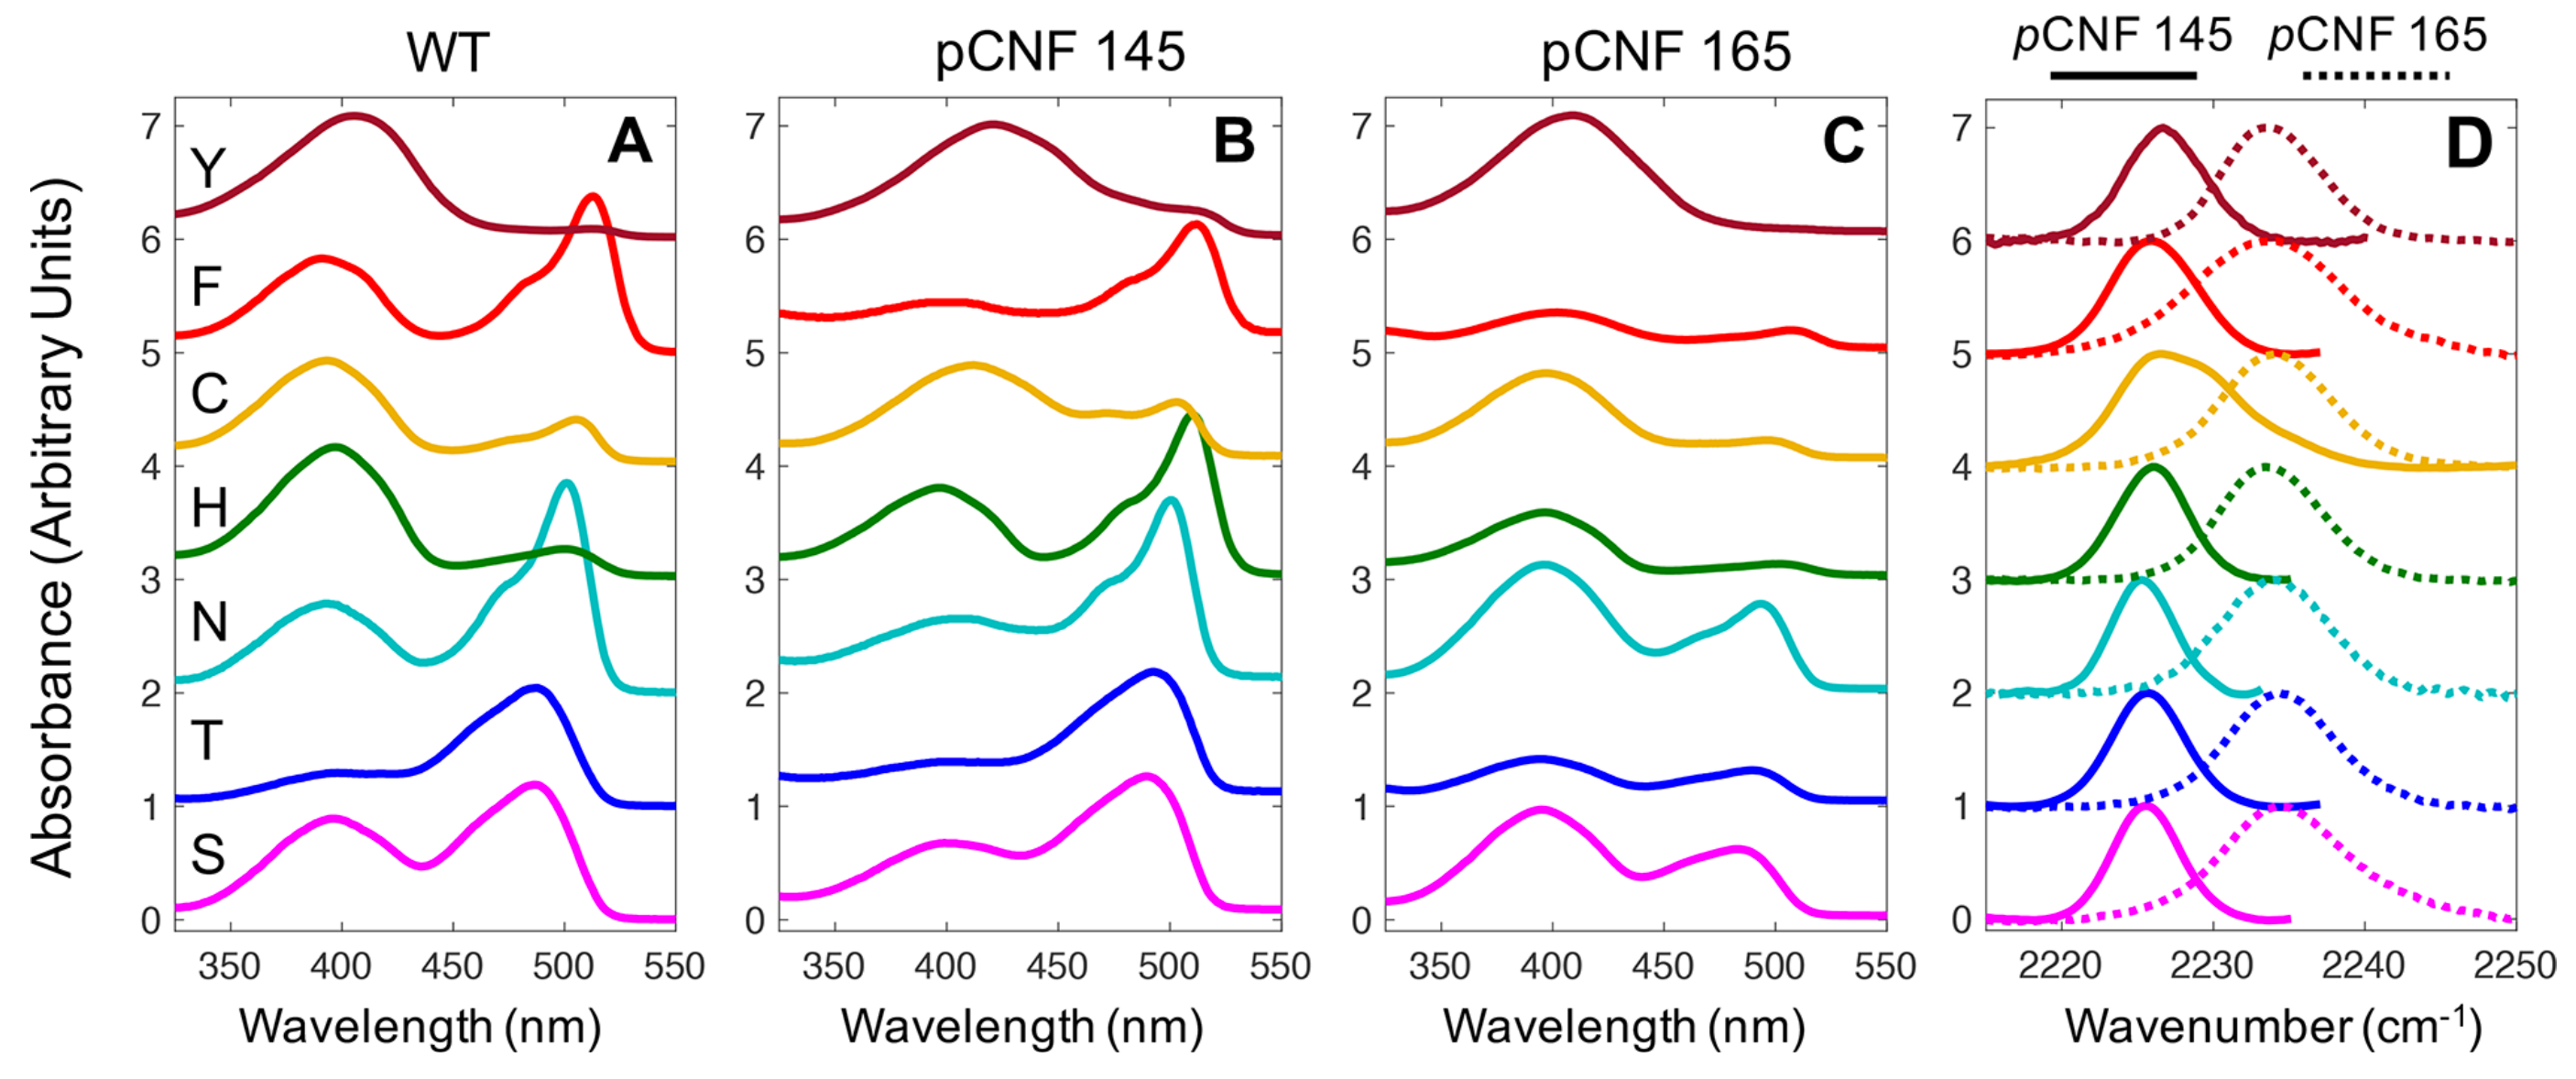
\includegraphics[width=\double]{figures-gfp-pKa/abs_spectra.png}
    \caption[Representative absorption spectra for all GFP mutants]{
        Representative absorption spectra for all GFP mutants recorded at pH 7.4. 
        Panels A, B, and C show the visible absorption of the GFP fluorophore normalized to the absorbance at 280 nm for proteins that have no nitrile probe (A), \pCNF{} at position 145 (B), and \pCNF{} at position 165 (C). 
        Different colors represent the different amino acid side chains at position 203 based on the one-letter code in panel A. 
        Panel D shows the FTIR absorption of the \pCNF{} residue at either position 145 (solid) or 165 (dashed) with the same colors to denote different amino acids at position 203. 
        All spectra have been offset on the $y$-axis for clarity.
    }
    \label{fig:abs_spectra}
\end{figure}

\subsection{Comparing \pKa{} Shifts to Electronic Stark Effect Shifts}

To compare the changes in fluorophore \pKa{} to changes in electric field experienced by the fluorophore, we plotted the \pKa{} changes for all unique pairs of the seven mutants against the corresponding changes in electric field experienced by the fluorophore (calculated from Equation \ref{eq:stark}) in Figure \ref{fig:pKa_vs_stark}.
The data in Figures \ref{fig:pKa_vs_stark}A-C were generated from GFP constructs that contained no nitrile probe (Figure \ref{fig:pKa_vs_stark}A), \pCNF{} at position 145 (Figure \ref{fig:pKa_vs_stark}B), or \pCNF{} at position 165 (Figure \ref{fig:pKa_vs_stark}C).
In this case, the seven individual \pKa{} values and deprotonated fluorophore absorption energies from the position 203 mutants gave rise to 21 distinct \pKa{} shifts and absorption energy changes.
We used these absorption energy changes and the known Stark tuning rate of the deprotonated GFP fluorophore to calculate the electric field changes experienced by the fluorophore from Equation \ref{eq:stark}.
For all of these comparisons, we observed a strong linear correlation between the fluorophore \pKa{} shifts and corresponding Stark effect shifts due to the position 203 mutations, which suggests that these two orthogonal measurements responded similarly to the same electrostatic perturbation.
More specifically, the mutations that caused large, positive electric field changes in the direction of the fluorophore difference dipole moment tended to cause concurrent increases in the fluorophore \pKa{} (to favor the neutral versus negatively charged form).
Conversely, mutations that caused large electric field changes anti-parallel to the difference dipole moment of the fluorophore tended to push the equilibrium toward the negative form of the fluorophore.
Furthermore, responses to electrostatic perturbations followed previously observed patterns based on the chemical identity of the mutant residue.
In Figure \ref{fig:pKa_vs_stark}, the different colors represent the type of mutation that was made at position 203 based on the key in Figure \ref{fig:pKa_vs_stark}A.
For instance, the magenta points represent mutations involving the replacement of an -OH side chain (T or S) with an aromatic side chain (F or Y), similar to the mutation made in yellow fluorescent protein \cite{Wachter1998}.
We previously observed that mutations of this nature, and their opposites (red in Figure \ref{fig:pKa_vs_stark}), are responsible for the largest changes in electric field, measured spectroscopically.
In this work, we see that these mutations also cause the largest shifts in \pKa{}.
Additionally, we saw that conservative mutations (e.g. S to T or F to Y; black in Figure \ref{fig:pKa_vs_stark}) tended to cause the smallest changes in both \pKa{} and electric field experienced by the fluorophore.
The observation that the Stark effect shifts and \pKa{} shifts of the fluorophore are not only linearly correlated, but also respond similarly to the same types of mutations (denoted by the colors in Figure \ref{fig:pKa_vs_stark}), gives us confidence that these two orthogonal probes of electrostatic perturbation are indeed reporting on a common electrostatic effect.

\begin{figure}
    \center
    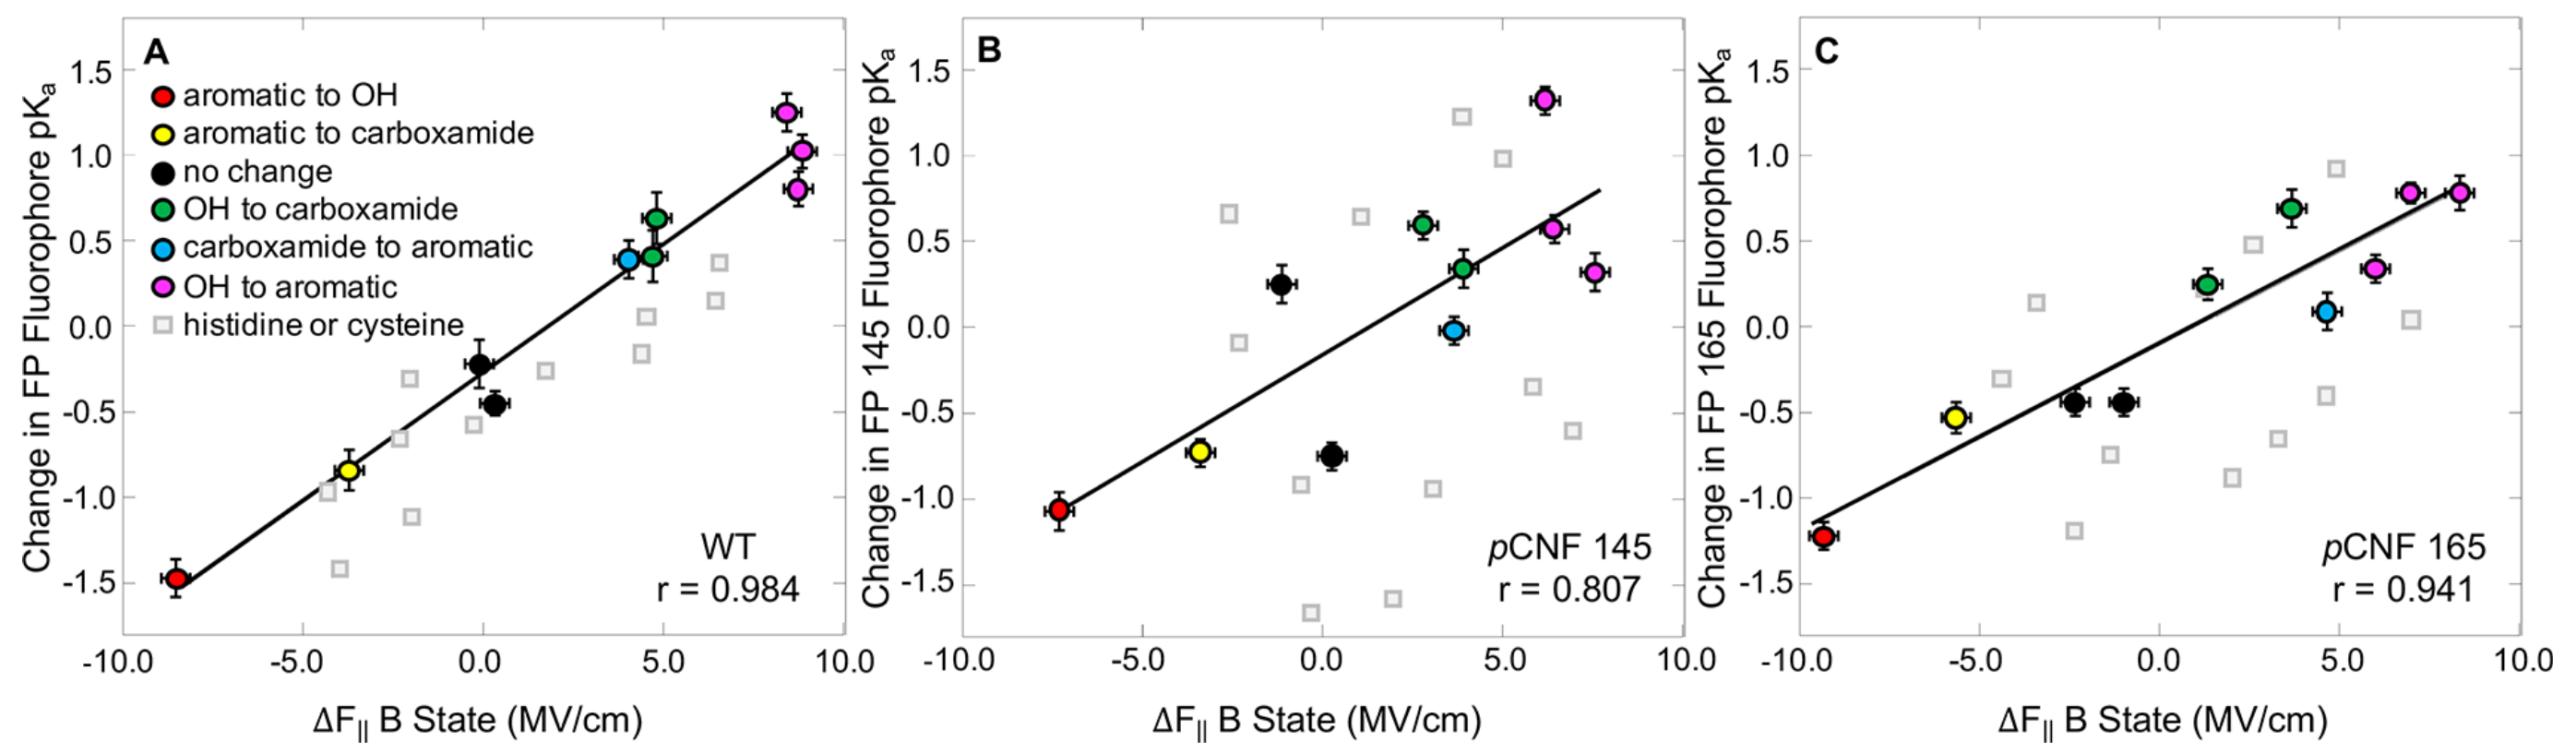
\includegraphics[width=\double]{figures-gfp-pKa/pKa_vs_elec_stark.png}
    \caption[Fluorophore \pKa{} compared to the field reported by the electronic transition of the fluorophore]{
        Changes in the measured fluorophore \pKa{} plotted against changes in the electric field experienced by the B state of the fluorophore for GFP mutants with (A) no nitrile probe present, (B) \pCNF{} at position 145, and (C) \pCNF{} at position 165. 
        Different colors represent the type of mutation that was made to position 203 based on the key in panel A. 
        Gray squares represent position 203 mutations that involved changes to or from histidine or cysteine and are omitted from the best fit lines and correlation constants. 
        Error bars on the $x$-axis represent uncertainty in the published Stark tuning rate of the deprotonated GFP fluorophore. 
        Error bars on the $y$-axis represent standard deviations in the inflection points of at least three \pKa{} titration curves.
    }
    \label{fig:pKa_vs_stark}
\end{figure}

In Figure \ref{fig:pKa_vs_stark}, however, there are clear deviations from this linear correlation.
In displaying the data in this manner, it is apparent that, with the exception of the proteins with no \pCNF{} probe (4A), mutations to or from histidine or cysteine (gray squares in Figure \ref{fig:pKa_vs_stark}) caused \pKa{} changes that were in poor agreement with the corresponding Stark effect shifts of the GFP fluorophore.
Of the seven side chains we placed at position 203, H and C are clearly different from the rest because they can be titrated near physiological pH (the \pKa{} values of H and C side chains in water are 6.0 and 8.1, respectively).
It is reasonable to suspect that the presence of a second titration site (H or C at position 203) might complicate the straightforward analysis of the GFP fluorophore equilibrium and contribute to the weakening of the correlations shown in Figures \ref{fig:pKa_vs_stark}B,C.
However, the fact that the disagreement between electronic Stark effects and \pKa{} shifts for these mutations is only apparent when either nitrile probe is present suggests that the presence of \pCNF{} is the cause of the disagreement.
Because of the likely role of hydrogen bonding to the fluorophore in determining its \pKa{}, and the ability of the nitrile group to accept a hydrogen bond, we think it is likely that \pCNF{} at either of these locations could potentially disrupt the hydrogen bonding network in the interior of GFP, which could in turn perturb the native \pKa{} values.
Further studies are underway to investigate changes in the hydrogen bonding network near the GFP fluorophore induced by the insertion of \pCNF{} residues at positions 145 and 165 to test this hypothesis.
In the sections that follow, we address the electrostatic perturbations induced by the nitrile probes and how they affect our ability to interpret the measured vibrational energies in a meaningful way.

\subsection{\pKa{} Perturbations Due to Nitrile Probes}

One of the principal criticisms of using nitrile vibrational probes in biological molecules is that the inclusion of the nitrile itself, an oscillator with a large ground state dipole moment and hydrogen bond accepting ability, will inherently perturb the biomolecule, and is not a reliably benign reporter of the molecular environment of interest \cite{Adhikary2014}.
The observation discussed above, that mutations to C or H deviate from the otherwise strong correlation between \pKa{} and Stark effect shift when a nitrile probe is present, may indeed be evidence of this effect.
To investigate this, we examined the ability of the nitrile probes to perturb the fluorophore \pKa{} values, relative to the values with no nitrile probe present.
This is shown in Figure \ref{fig:pKa_sidechain}, where the change in fluorophore \pKa{} of all position 203 mutants (indicated by the one letter code on the $x$-axis) is plotted as a function of a nitrile located at either position 145 (black) or 165 (red).
For most of the mutants, we saw that the insertion of a \pCNF{} residue at either position induced a \pKa{} change of at least $\pm$ 0.2 pH units, which represents a significant electrostatic perturbation due to the nitrile probe.
Because the nitrile moiety can accept a hydrogen bond from either water or a nearby amino acid residue, inserting \pCNF{} into the \textbeta{}-barrel of GFP has the potential to disrupt the hydrogen bonding network around the fluorophore, which could explain the significant \pKa{} changes in Figure \ref{fig:pKa_sidechain}.
C203 mutants with either nitrile probe clearly exhibit the largest observed \pKa{} shifts, up to 1 pH unit, which further supports our decision to remove C203 from the trends in Figure \ref{fig:pKa_vs_stark}.
This highlights the care that should be taken when using nitriles as electrostatic probes.

\begin{figure}
    \center
    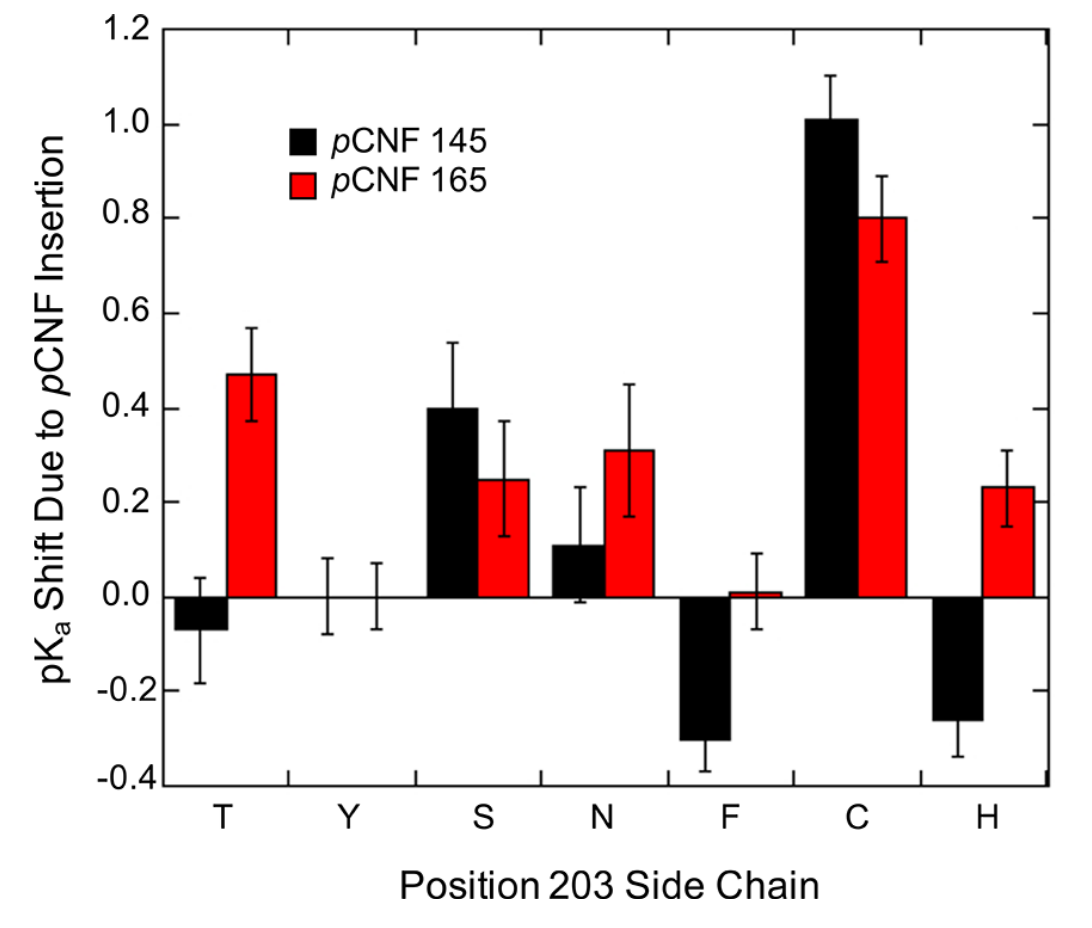
\includegraphics[width=\single]{figures-gfp-pKa/pKa_by_side_chain.png}
    \caption[\pKa{} shifts due to the insertion of \pCNF{}]{
        \pKa{} shift of the GFP fluorophore caused by the insertion of \pCNF{} at position 145 (black) or 165 (red) for each amino acid at position 203 (one letter code on the $x$-axis). 
        Error bars represent the standard deviation of at least three titrations.
    }
    \label{fig:pKa_sidechain}
\end{figure}

In contrast, the \pCNF{} residues appear to perturb the chromophore environment the least when Y or F is at position 203.
Previous work has suggested that aromatic van der Waals interactions between the residue at position 203 and the fluorophore, as well as specific hydrogen bonding to and from the fluorophore, are the dominating contributions to GFP fluorophore \pKa{} \cite{Elsliger1999}.
As such, we think that the mutants containing Y or F at position 203 have \pKa{} values that are dominated by aromatic interactions, and thus should be less sensitive to subtle changes in the surrounding hydrogen bonding network.
Therefore, with the view that the perturbations shown in Figure \ref{fig:pKa_sidechain} were caused by differences in the hydrogen bonding network around the fluorophore due to the \pCNF{} residues, it makes sense that the smallest perturbations were observed for mutants with Y or F at position 203.
This is further supported by the elevated \pKa{} values we measured for the Y203 and F203 mutants ($\sim$7.5-8.0; Table \ref{tbl:pKas}), which suggest that aromatic interactions between Y203 or F203 and the fluorophore work to stabilize the protonated form of the fluorophore.
Interestingly, with the exception of F203 and H203 mutants containing \pCNF{} 145, the insertion of the nitrile probe either caused no measurable \pKa{} change or caused a shift to higher \pKa{} values (in favor of the neutral fluorophore).
While it is difficult to ascribe this general increase in fluorophore \pKa{} to any specific interactions, it may be the result of favorable aromatic interactions between the fluorophore and the nearby \pCNF{} 145 or 165.
Additionally, the inserted nitrile probes might disrupt the hydrogen bonding environment around the fluorophore in a systematic way that tends to favor the neutral fluorophore. 

\subsection{Comparing \pKa{} Shifts to Vibrational Stark Effect Shifts}

As we have observed before, \pCNF{} at positions 145 and 165 can perturb the native environment around the GFP fluorophore.
However, regardless of the mechanism by which these nitrile probes shift the \pKa{} of the GFP fluorophore, our primary interest is in relating changes in their measured vibrational energies to changes in electric field via Equation \ref{eq:stark}.
We previously observed that, even though \pCNF{} introduced large electric field perturbations into GFP, changes in the nitrile absorption energy could still be related to electric field changes that were verified by an independent electric field reporter \cite{Slocum2016}.
We hypothesized that a similar effect might happen here, where the observed \pKa{} perturbations due to \pCNF{} 145 and 165 might be cancelled out such that differences in \pKa{} can still be correlated to VSE shifts of the nitriles.
To investigate this possibility, we directly compared the nitrile Stark effect shifts to the \pKa{} shifts of the fluorophore, caused by the mutations at position 203.
Figure \ref{fig:pKa_vs_cnf} shows the fluorophore \pKa{} changes due to all unique pairs of the seven position 203 mutants plotted against the corresponding electric field changes projected onto either \pCNF{} 145 (Figure \ref{fig:pKa_vs_cnf}A) or 165 (Figure \ref{fig:pKa_vs_cnf}B) calculated from Equation \ref{eq:stark} using the nitrile absorption energies as determined from Figure \ref{fig:abs_spectra}D.
Similar to the data shown in Figure \ref{fig:pKa_vs_stark}, we observed a linear correlation between the \pKa{} shifts and the corresponding electric field changes experienced by the \pCNF{} residues, which further strengthens our confidence in the ability of these two orthogonal measurements to report on the same electrostatic perturbations.
Additionally, based on the color key in Figure \ref{fig:pKa_vs_cnf}B, we saw that the same trends in position 203 side chain that were observed from the fluorophore Stark effect response (Figure \ref{fig:pKa_vs_stark}) were observed in the responses of these nitrile probes.
The trend lines in Figure \ref{fig:pKa_vs_cnf}A and \ref{fig:pKa_vs_cnf}B have slopes that differ in both sign and magnitude, which highlights the geometric dependence of the vibrational Stark effects shifts (dot product in Equation \ref{eq:stark}).
Because \pCNF{} 145 and 165 are spatially removed from each other and oriented in different directions (Figure \ref{fig:system}), we should not expect the projection of an electric field change on to their respective bond axes to result in the same changes in energy.

\begin{figure}
    \center
    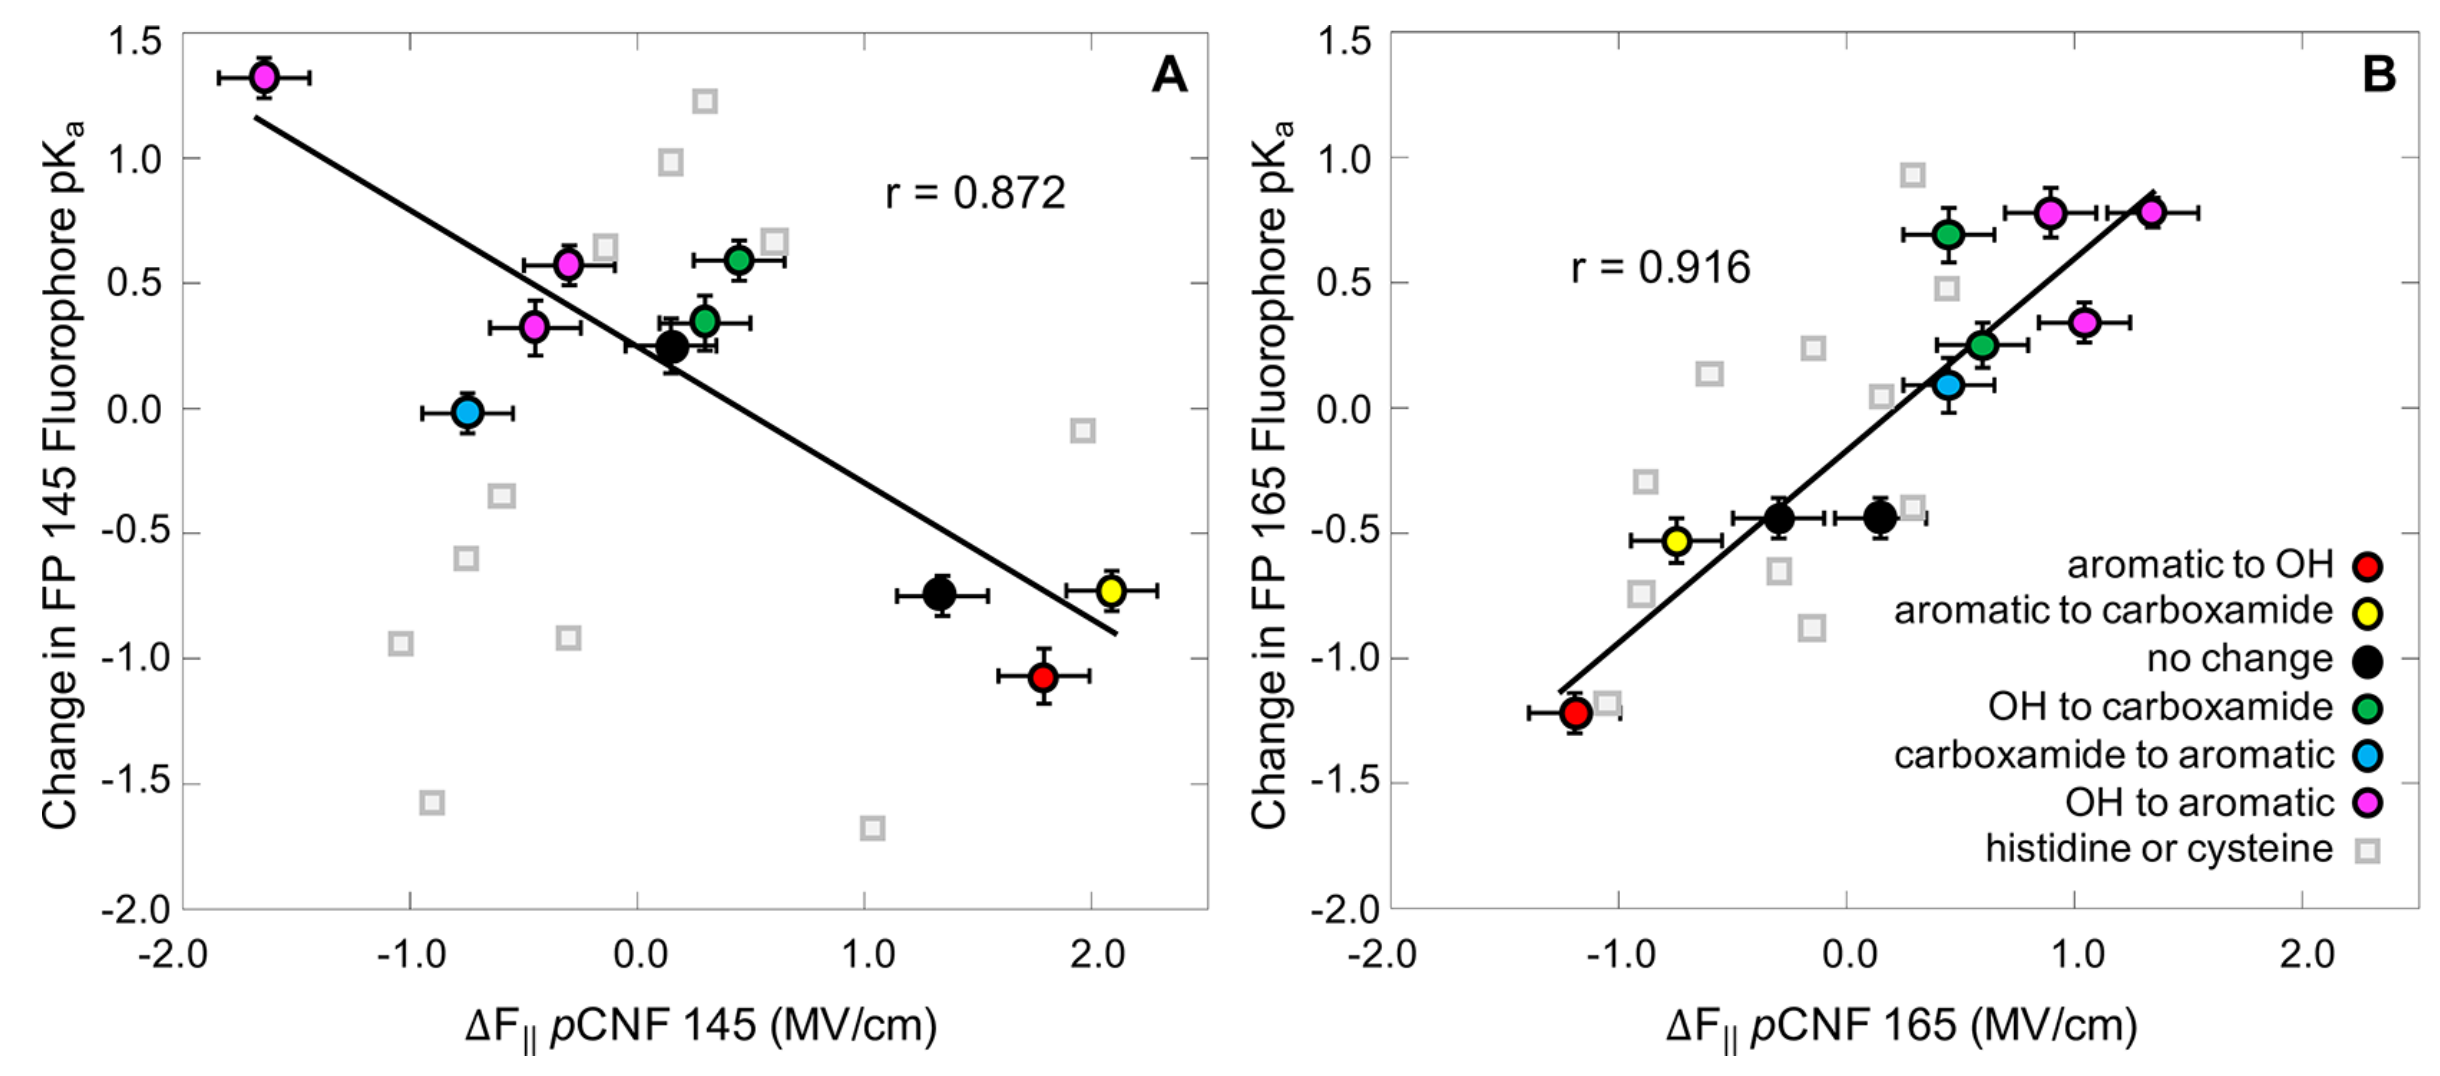
\includegraphics[width=\double]{figures-gfp-pKa/pKa_vs_cnf.png}
    \caption[Fluorophore \pKa{} compared to the field reported by \pCNF{} nitrile frequencies]{
        Changes in the fluorophore \pKa{} plotted against the electric field changes measured from \pCNF{} 145 (A) and 165 (B) for all unique pairs of the seven position 203 mutants. 
        Colors represent the type of mutation made to position 203 based on the key in panel B. 
        Gray squares represent position 203 mutations that involved changes to or from histidine or cysteine and are omitted from the best fit lines and correlation constants. 
        Error bars on the $x$-axis represent uncertainty in the published Stark tuning rate of \pCNF{}. 
        Error bars on the $y$-axis represent standard deviations in the inflection points of at least three titration curves.
    }
    \label{fig:pKa_vs_cnf}
\end{figure}

The observed linear correlation between VSE shifts of these inserted nitriles and the corresponding fluorophore \pKa{} shifts is remarkable.
In the previous section, we showed that \pCNF{} 145 and 165 can significantly perturb the fluorophore \pKa{} values (Figure \ref{fig:pKa_sidechain}), and yet the changes in \pKa{} are still well correlated to the measured VSE shifts (Figure \ref{fig:pKa_vs_cnf}).
This is similar to what we have previously reported, where \pCNF{} residues at these positions in GFP cause a significant electrostatic perturbation to the fluorophore, but do not affect GFP's intrinsic fluorescence sensitivity to the position 203 mutations \cite{Slocum2016}.
The perturbations caused by \pCNF{} residues in GFP appear to be systematic, such that the comparison between two states allows any perturbations caused by the experiment itself to be cancelled and the resulting energy difference to be interpreted in a meaningful way.
However, again it is clear that mutations to or from cysteine and histidine caused a weakening in the correlation between the \pKa{} shifts and the electric fields measured from each \pCNF{} residue, although the effect is worse for \pCNF{} 145 than it is for \pCNF{} 165. 

Because of our assertion that the \pKa{} and Stark effect shifts represent orthogonal responses to the same electrostatic perturbations, we wanted to explore the idea that the nitrile frequencies might simply shift as a result of differences in the concentration of protonated and deprotonated fluorophores.
For instance, if the A and B states of the fluorophore exert different electric fields onto the nearby \pCNF{} at position 145 or 165, then the frequency changes might simply reflect different ratios of the two field contributions from the A and B states.
In this case, the frequency shifts that we measured might be dominated by the A and B state contributions, not the changes in electrostatic environment due to the position 203 mutations.
However, it seems unlikely that the \pCNF{} 145 probes are sensitive to the mixed populations of A and B states given their extremely narrow linewidths ($\sim$5-6 \si{\wn}, except for C203; Figure \ref{fig:abs_spectra}A).
On the other hand, the \pCNF{} 165 probes were somewhat more broad ($\sim$8-9 \si{\wn}) and could conceivably contain contributions from both the A and B state fields.
To test whether the \pCNF{} 165 spectra was convolved with overlapping A and B state contributions, we measured the pH dependence of the \pCNF{} 165 absorption for the mutant containing T203.
Figure \ref{fig:cnf_vs_pH} shows the resulting spectra over the range of pH 7-9.
We measured no detectable change in the center frequency, which we interpret to mean that the \pCNF{} 165 was insensitive to the mixed population of A and B states.
Thus, we believe that differences in the measured nitrile frequencies are dominated by the electrostatic perturbation of the position 203 mutations. 

\begin{figure}
    \center
    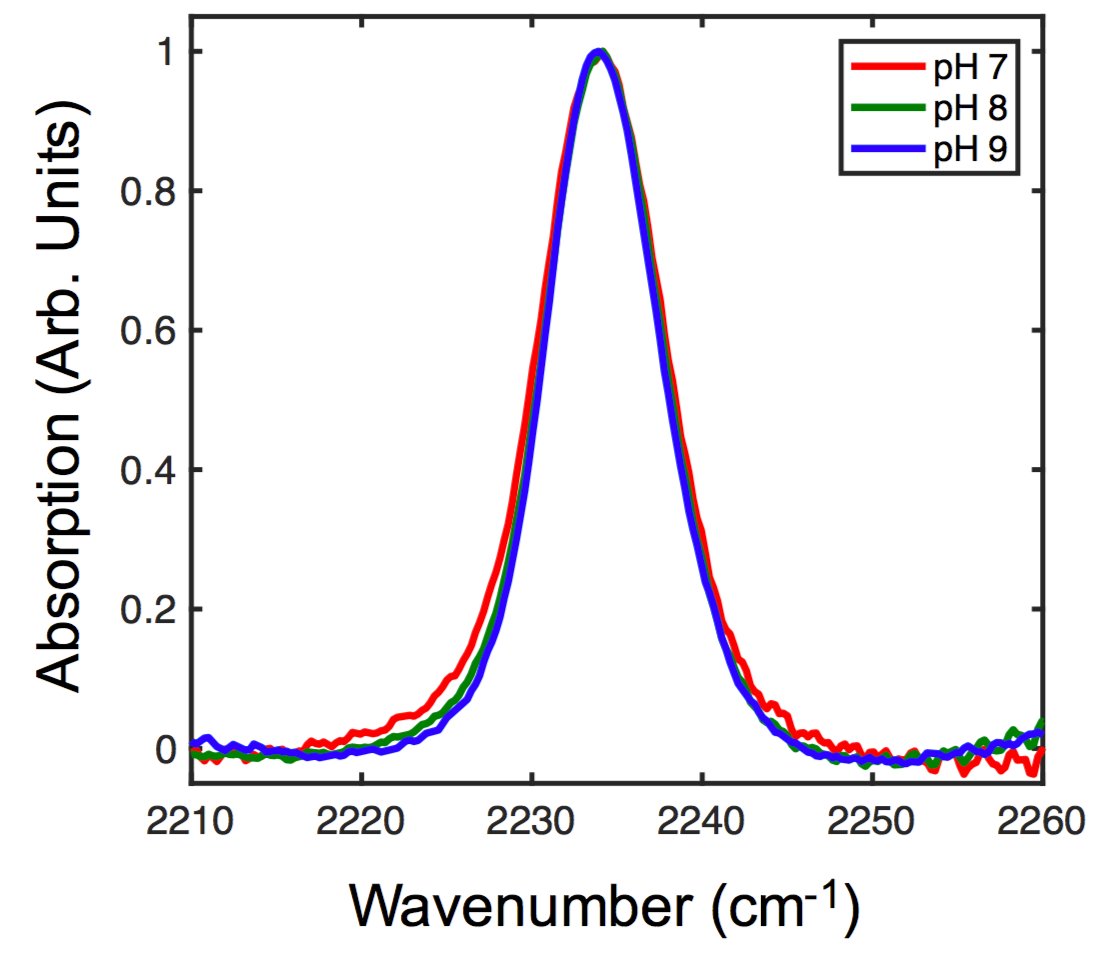
\includegraphics[width=\single]{figures-gfp-pKa/cnf_vs_pH.png}
    \caption[Nitrile absorption spectra at various pH levels]{
        Nitrile absorption spectra as a function of pH for the mutant containing threonine at position 203 and \pCNF{} at position 165. 
        No detectable change in the center frequency was measured between pH 7-9.
    }
    \label{fig:cnf_vs_pH}
\end{figure}

One additional concern with comparing the nitrile VSE shifts to the \pKa{} shifts of the \pCNF{}-containing GFP mutants is the difference in protein concentration with which both experiments were performed.
Because of the low absorption cross section of the nitrile stretch, the protein was concentrated to $\sim$1 mM to achieve adequate signal of the nitrile VSE probe for FTIR measurements. 
In contrast, the \pKa{} measurements were carried out at much lower concentrations ($\sim$10-100 $\mu$M) to ensure that the visible absorption of the GFP fluorophore did not fall outside of the linear range of Beer's law absorption.
This is potentially problematic because of the known propensity of GFP to dimerize at high concentrations and the fact that dimerization affects the GFP fluorophore equilibrium \cite{Tsien1998}.
To test whether the measured \pKa{} values of the variants of GFP used here exhibited a strong dependence on protein concentration, we measured the \pKa{} values of two mutants at concentrations of $\sim$1 mM to mimic the high concentration of the FTIR measurements.
As seen in Figure \ref{fig:conc_depend}, the ratio of A to B state absorption can change drastically as a function of concentration.
However, the pH dependence of the fluorophore absorption at high concentrations still yields \pKa{} values (estimated from Equation \ref{eq:sigmoid}) that are within experimental error of those measured for the same protein at lower concentrations.
This result suggests that, while dimerization can affect the relative amount of A versus B state in the interior of the protein, the midpoint of the equilibrium used in these Stark-\pKa{} comparisons remains unchanged.
All together, these observations suggest that the Stark effect shifts and \pKa{} shifts in GFP responded similarly to the same electrostatic perturbations in an orthogonal fashion.

\begin{figure}
    \center
    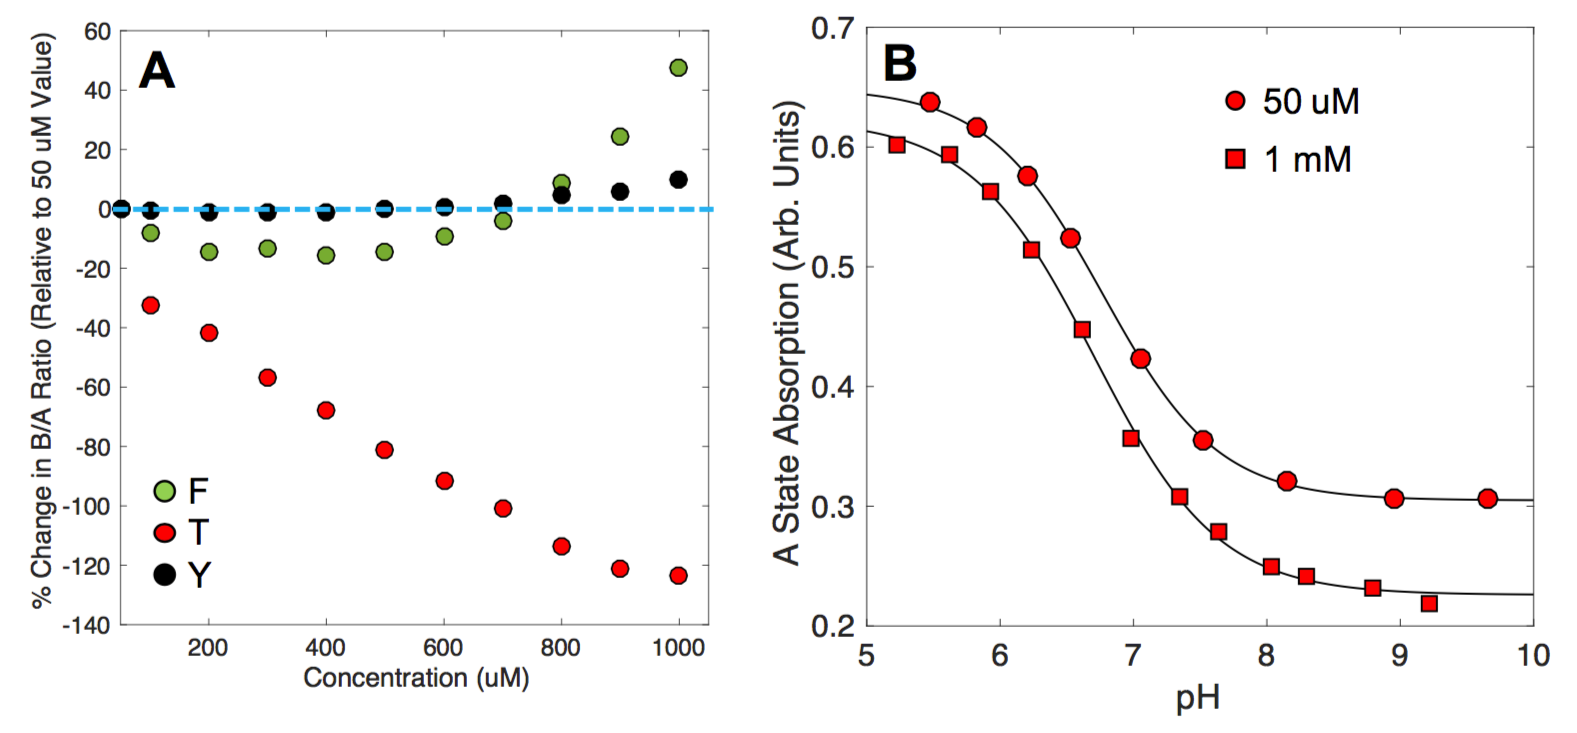
\includegraphics[width=\double]{figures-gfp-pKa/concentration_dependence.png}
    \caption[Effect of protein concentration on GFP fluorophore equilibrium]{
        The effect of protein concentration on GFP fluorophore equilibrium. 
        (A) The percentage change in the ratio of A to B state absorption as a function of protein concentration. 
        The colors represent a different amino acid at position 203 based on the key. 
        (B) The A state titration of wild type superfolder GFP (red data points from (A)) at low (circles) and high (squares) concentrations. 
        Both titrations give inflection points that are within experimental error of each other (\pKa{} = 6.7).
    }
    \label{fig:conc_depend}
\end{figure}

In summary, we observed that similar types of mutations at position 203 caused similar changes in (1) the vibrational absorption energies of inserted nitrile probes; (2) the visible absorption energies of the GFP fluorophore; and (3) the fluorophore \pKa{} values.
The self-consistency in these three orthogonal experimental measurements of electrostatic perturbation from the position 203 mutations makes this experimental dataset an ideal benchmark for computational models that predict electrostatic fields in proteins.

\subsection{Computational Prediction of Fluorophore \pKa{} }

Because of the potential for these orthogonal measurements to serve as benchmarks for electrostatics models, we tested the ability of a common continuum electrostatics model to reproduce these site-specific electric field changes and the corresponding fluorophore \pKa{} shifts.
To do this we carried out a series of electrostatic free energy calculations of the GFP fluorophore equilibrium.
Here we outline our strategy; for a detailed theoretical background on the calculation of \pKa{} values using APBS, we refer the reader to several recent reviews \cite{Baker2005, Baker2004, Baker2001, Wagoner2004, Unni2011}.

The change in \pKa{} of the GFP fluorophore ($\Delta$\pKa{}), relative to its value in aqueous buffer, may be calculated as the difference in free energies of association between the fluorophore in an aqueous environment ($\Delta_aG_\text{free}$) and the fluorophore in the protein environment ($\Delta_aG_\text{protein}$), as shown in Equation \ref{eq:ddG}, where $R$ is the ideal gas constant and $T$ is the temperature.
\begin{equation}
    \Delta \pKa = \frac{\Delta_aG_\text{free}}{RT \ln 10} - \frac{\Delta_aG_\text{protein}}{RT \ln 10} = \frac{\Delta\Delta_aG}{RT \ln 10}
    \label{eq:ddG}
\end{equation}
While Equation \ref{eq:ddG} gives an exact relationship for $\Delta$\pKa{}, it is difficult to directly evaluate the $\Delta_aG_\text{free}$ and $\Delta_aG_\text{protein}$ terms.
Therefore, the $\Delta$\pKa{}, or analogously $\Delta\Delta_aG$, is typically calculated indirectly via the thermodynamic cycle shown in Equation \ref{eq:dGxfer} and illustrated in Figure \ref{fig:thermocycle}.
\begin{equation}
    \begin{split}
    \Delta\Delta_a G &= \Delta_a G_{\text{free}} - \Delta_a G_{\text{protein}} \\
    &= \Delta G_{\text{xfer}_B} - \Delta G_{\text{xfer}_A}
    \end{split}
    \label{eq:dGxfer}
\end{equation}
In Equation \ref{eq:dGxfer}, $\Delta G_{\text{xfer}_A}$ and $\Delta G_{\text{xfer}_B}$ represent the free energies of transferring the A and B states, respectively, of the fluorophore from an aqueous environment to the protein environment.
While the general approach illustrated in Figure \ref{fig:thermocycle} may be common, there are many different strategies for calculating the electrostatic free energy.
Here, we wanted to test whether the electrostatic free energies, calculated using APBS by solving the linear Poisson-Boltzmann (PB) equation:
\begin{equation}
    \nabla \cdot \epsilon(\vec{r}) = \epsilon(\vec{r})\bar{\kappa}^2\phi(\vec{r}) - 4\pi\rho(\vec{r})
    \label{eq:PB}
\end{equation}
could be used in Equation \ref{eq:dGxfer} to accurately reproduce the experimentally measured \pKa{} values of the GFP fluorophore. 
In Equation \ref{eq:PB}, $\epsilon(\vec{r})$ is the dielectric constant as a function of the position vector $\vec{r}$, $\phi(\vec{r})$ is the potential as a function of position, $\bar{k}^2$  is the ion accessibility coefficient, and $\rho(\vec{r})$ is the position dependent charge density. 

\begin{figure}
    \center
    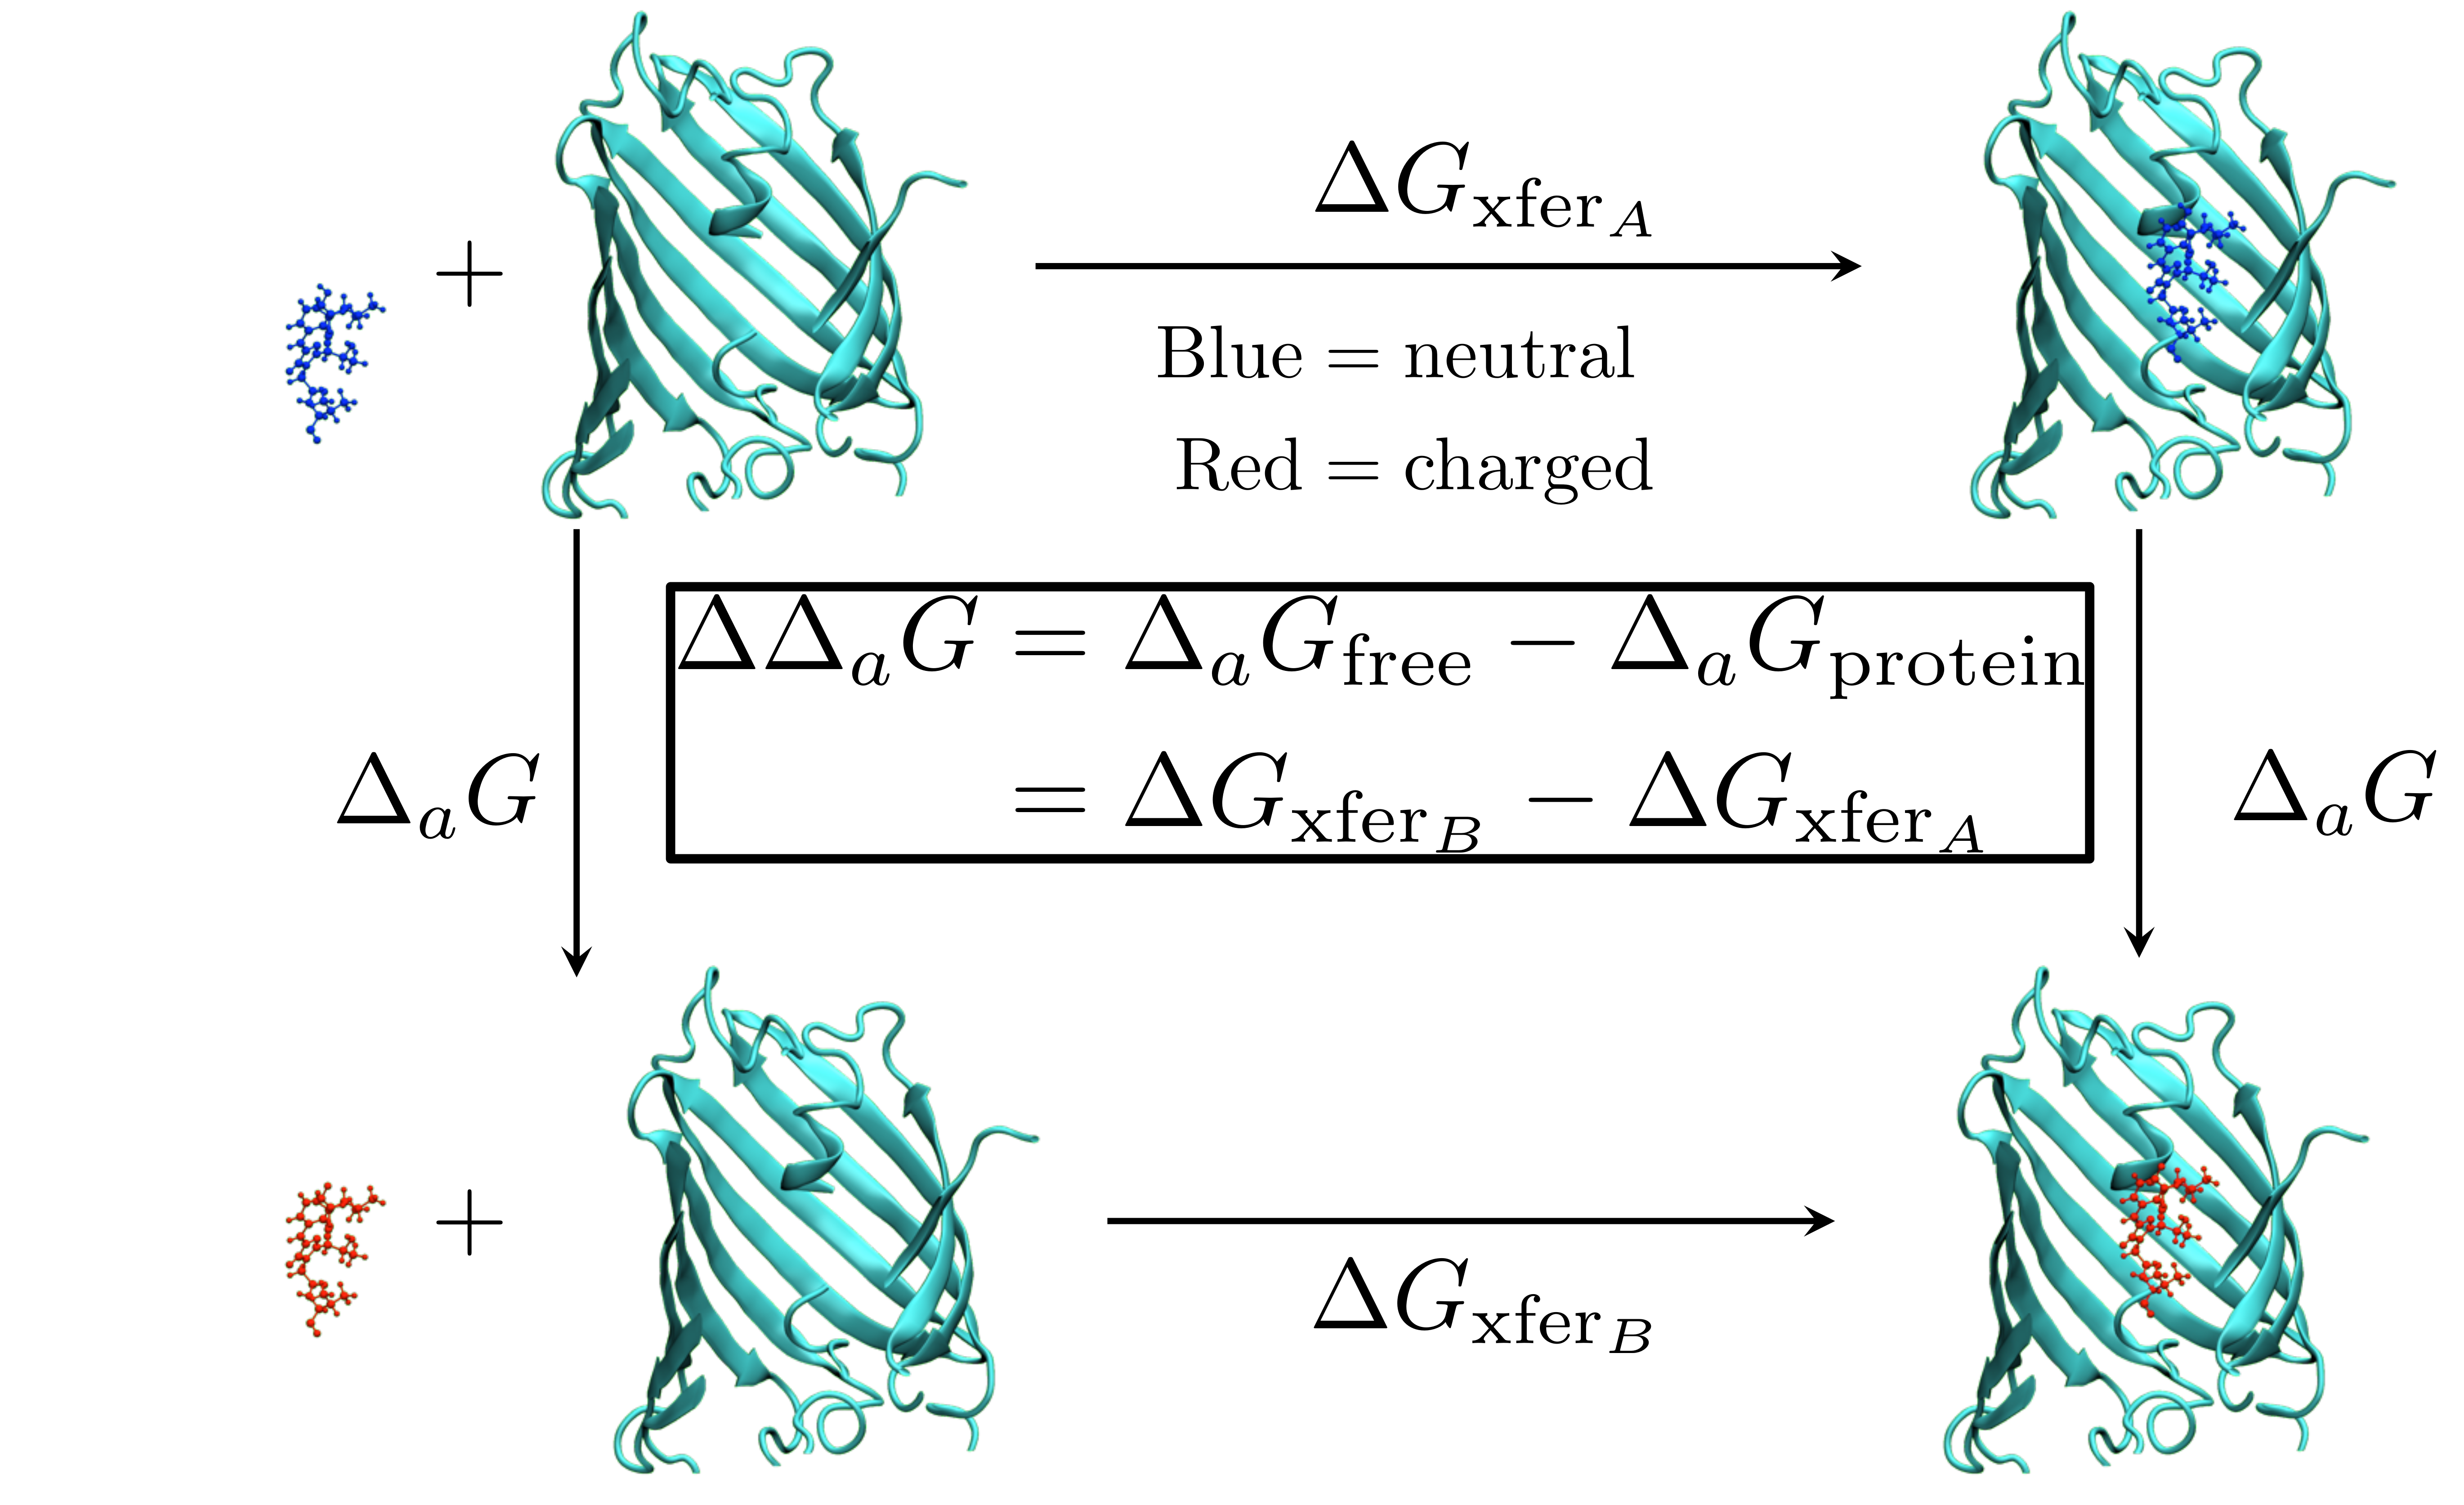
\includegraphics[width=\single]{figures-gfp-pKa/thermocycle.png}
    \caption[Schematic of the themodynaic cycle used for \pKa{} calculuations]{
        Cartoon representation of the thermodynamic cycle used for \pKa{} calculations. 
        The A and B states of the fluorophore are shown in blue and red, respectively. 
        The GFP structure is shown as a cyan cartoon.
    }
    \label{fig:thermocycle}
\end{figure}

Specifically, we wanted to evaluate the performance of APBS to reproduce the fluorophore \pKa{} values using minimal optimization to the commercially-available software package. 
We first performed the free energy calculations on the static starting structures that were modelled by homology from crystal structure 2b3p. 
The solvent was treated implicitly with a dielectric constant of 78.54 and the crystallized atoms were treated with a dielectric constant of 20, which is thought to be an effective protein dielectric in static structure calculations \cite{Mehler1999}.
While removing all explicit water molecules and replacing them with a continuum dielectric has been shown to be an accurate approximation in the continuum treatment of compact globular proteins \cite{Kukic2013, Simonson1996}, it may not necessarily hold for the \textbeta{}-barrel of GFP, which contains many confined water molecules that form intricate hydrogen bonded networks with other waters and protein residue side chains. These confined waters near the fluorophore likely play a large role in determining the \pKa{} through both structural and electrostatic effects.
Therefore, any crystallized waters within a 5 \si{\angstrom} sphere around the fluorophore phenol (or phenolate) oxygen were treated explicitly.
The results from these calculations are shown in Figure \ref{fig:calc_pKas}A, where we observed a poor correlation between the calculated and experimental \pKa{} values ($r = 0.27$).
We hypothesized that this was due to insufficient protein relaxation around the residue of mutation.
For example, inserting a nitrile probe at either position 145 or 165 often caused steric clash with nearby residues.
MD would add the protein relaxation into the model and eliminate this concern.
Additionally, we wanted to model protein fluctuations because PB-based calculations are extremely sensitive to protein configuration.

\begin{figure}
    \center
    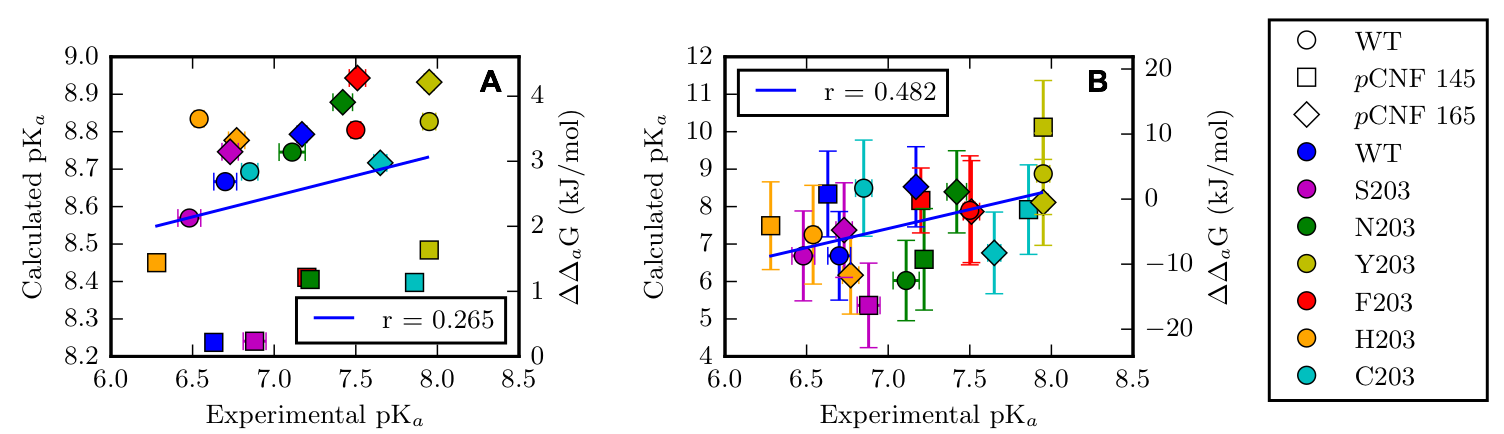
\includegraphics[width=\double]{figures-gfp-pKa/calc_pKas.png}
    \caption[Calculated \pKa{} values compared to experimental \pKa{} values]{
        Correlations between experimentally measured \pKa{} values and those calculated in APBS. 
        In both cases, the calculated \pKa{} is shown on the $y$-axis and the experimental \pKa{} is on the $x$-axis. 
        Data points shown as circles represent the mutant constructs with no nitrile probe, squares are the mutants with \pCNF{} at position 145, and diamonds are the mutants with \pCNF{} at position 165. 
        Error bars on the $x$-axis are small relative to the size of the data points. 
        (A) Correlation between experimental and calculated \pKa{} for APBS calculations performed on the modeled starting structures with the inclusion of explicit water molecules within a 5 \si{\angstrom} radius of the phenolic oxygen of the fluorophore as described in the main text. 
        (B) Correlation between experimental and calculated \pKa{} for APBS calculations performed on snapshots of 50 ns of MD simulation with the inclusion of explicit water molecules within a 5 \si{\angstrom} radius of the phenolic oxygen of the fluorophore.
    }
    \label{fig:calc_pKas}
\end{figure}

To account for the sensitivity of the calculation to the protein configuration, we performed MD simulations on the protein structures (including explicit solvation with TIP3P water) to generate an ensemble of reasonable structures that might exist during the course of a room temperature steady-state experiment.
We first wanted to validate our parameters for the GFP fluorophore and the surrounding titratable residues (namely E222 and H148) to ensure that the MD simulations gave a reasonable ensemble of protein configurations.
Specifically, for GFP mutants containing the TYG fluorophore (used in the present study), there is detailed crystallographic evidence of the complex hydrogen bonding network around the fluorophore, which we used as a basis for comparison for our ensemble of protein configurations \cite{Elsliger1999}.
Table \ref{tbl:crystal} lists 17 different hydrogen bonding interactions that were observed in the crystal structure of an analogous GFP mutant near the embedded fluorophore, as well as the corresponding interactions from our 50 \si{\ns} of MD simulation of wild type superfolder GFP.
We observed all 17 hydrogen bonding interactions in our simulations.
While most interactions were captured by the simulations to within < 1 \si{\angstrom} of the distances measured from the crystal structure, there were a few notable differences.
In our simulations, Q69 and Q94 were both further away from the fluorophore, which gave rise to interaction distances to the atoms in those residues that were greater than the distances predicted by the crystal structure.
This is likely due to the difference in amino acid sequence between the present study and the crystal structure that was used for comparison, or the fact that the crystal structure only represents a single, low energy conformation of the protein.
Interestingly, simulations with negatively charged E222 and H148 protonated at the N$_{\varepsilon}$ were not able to accurately reproduce these 17 hydrogen bonding interactions (data not shown).
Overall, the fact that our MD simulations were able to accurately capture most of the experimentally observed hydrogen bonding interactions around the fluorophore suggests that we used reasonable parameters for the GFP fluorophore and supports our decision to protonate E222 and the N$_\delta$ of H148.
However, there is no structural data available for any of the position 203 mutants or the mutants with \pCNF{} 145 or 165.

\begin{table}
    \caption[Observed hydrogen bonding interactions in MD simulation compared to in crystal structure]{
        Hydrogen bonds around the GFP fluorophore in the A and B states. 
        Donor and acceptor columns designate the hydrogen bond donor and acceptor. 
        Distances from crystallographic evidence are shown for each interaction and taken from ref \citenum{Elsliger1999}. 
        The MD column represents the same interaction distances over the course of 50 ns of MD simulation. 
        Error bars represent the standard deviation of the distance throughout the simulation. 
        For interactions involving water, the minimum distance to the oxygen of water is presented.
    }
    \begin{center}
        \resizebox{\double}{!}{
    \begin{tabular}{cc|cc|cc|cc}
    \toprule
    \multicolumn{4}{c}{A State}                                         & \multicolumn{4}{c}{B State}\\
    \toprule
    
    Donor                  & Acceptor              & Crystal (\AA) & MD (\AA) & Donor             & Acceptor                  & Crystal (\AA) & MD (\AA) \\
    \midrule{}
     Chro OH               & T203 O                & 3.0 & $4.2 \pm 0.6$ & T203 O$_\gamma$         & Chro \ce{O-}             & 2.6 & $ 3.4  \pm 0.9  $ \\
    \ce{H2O}               & Chro OH               & 2.5 & $2.8 \pm 0.2$ & H148 N$_\delta$         & Chro \ce{O-}             & 2.9 & $ 3.0  \pm 0.2  $ \\
    R168 N                 & H148 N$_\varepsilon$  & 3.2 & $3.2 \pm 0.2$ & R168 N                  & H148 N$_\varepsilon$     & 3.2 & $ 3.1  \pm 0.2  $ \\
    H148 N$_\delta$        & N146 O                & 2.6 & $2.9 \pm 0.2$ & \ce{H2O}                & Chro \ce{O-}             & 2.6 & $ 2.8  \pm 0.2  $ \\
    \ce{H2O}               &  N146 O               & 3.2 & $3.0 \pm 0.3$ & \ce{H2O}                & N146 O                   & 2.9 & $ 2.8  \pm 0.2  $ \\
    S205 OG                & \ce{H2O}              & 2.6 & $2.8 \pm 0.2$ & S205 O$_\gamma$         & \ce{H2O}                 & 2.7 & $ 2.8  \pm 0.2  $ \\
    E222 O$_{\varepsilon 2}$  & Chro O$_{\rm{T}64\gamma}$  & 2.8 & $2.8 \pm 0.2$ & E222 O$_{\varepsilon2}$ & Chro O$_{\rm{T}64\gamma} $    & 2.8 & $ 3.0  \pm 0.7  $ \\
    \ce{H2O}               & E222$_{\varepsilon 1}$ & 2.4 & $2.9 \pm 0.2$ & Chro O$_{\rm{T}64\gamma} $   & V61 O                    & 3.0 & $ 3.1  \pm 0.2  $ \\
    Chro O$_{\rm{T}64\gamma} $  & V61 O                 & 3.0 & $3.0 \pm 0.2$ & \ce{H2O}           &  E222 O$_{\varepsilon1}$ & 2.4 & $ 2.8  \pm 0.2  $ \\
    Q69 N$_\varepsilon$    & \ce{H2O}              & 2.7 & $3.0 \pm 0.2$ & Q69 N$_\varepsilon$     & \ce{H2O}                 & 2.8 & $ 3.0  \pm 0.2  $ \\
    Q183 N$_\varepsilon$   & Q69 O$_\varepsilon$  & 3.1 & $6.7 \pm 1.1$ & Q183 N$_\varepsilon$     & Q69 O$_\varepsilon$       & 3.2 & $ 6.2  \pm 0.7  $ \\
    Q94 N$_\varepsilon$    & Chro O$_\text{ima}$   & 3.0 & $4.9 \pm 0.7$ & R96 N$_\varepsilon$     & Q183 O$_\varepsilon$     & 3.0 & $ 4.0  \pm 1.3  $ \\
    R96 N$_{\eta 1}$       & Chro O$_\text{ima}$   & 3.0 & $3.0 \pm 0.3$ & R96 N$_{\eta 1}$        & Q183 O$_\varepsilon$     & 2.9 & $ 4.0  \pm 1.3  $ \\
    R96 N$_{\eta 1}$       & Q183 O$_\varepsilon$  & 2.9 & $3.9 \pm 0.3$ & Q94 N$_\varepsilon$     & Chro O$_\text{ima}$      & 3.0 & $ 5.1  \pm 0.4  $ \\
    R96 N$_\varepsilon$    & Q183 O$_\varepsilon$  & 2.9 & $2.9 \pm 0.2$ & R96 N$_{\eta 1}$        & Chro O$_\text{ima}$      & 2.7 & $ 2.8  \pm 0.1  $ \\
    R96 N$_{\eta 2}$       & T62 O                 & 2.6 & $3.0 \pm 0.3$ & R96 N$_{\eta 2}$        & T62 O                    & 2.7 & $ 3.0  \pm 0.2  $ \\
    R96 N$_{\eta 2}$       & \ce{H2O}              & 2.9 & $2.9 \pm 0.2$ & R96 N$_{\eta 2}$        & \ce{H2O}                 & 2.8 & $ 3.0  \pm 0.1  $ \\
    \bottomrule
    \end{tabular}
}
    \end{center}
    \label{tbl:crystal}
\end{table}

To further validate our model parameters for the fluorophore and positions 145, 165, and 203, we followed the RMS deviations of each mutant protein relative to its minimized starting structure over the course of a 50 \si{\ns} trajectory of MD simulation.
These results are shown in Figure \ref{fig:rmsd} in the Supporting Information, where we observed that the backbone RMS deviations remained low (< 2.7 \si{\angstrom}) throughout the protein trajectory for all 42 simulations.
This suggests that single point mutations to position 203 and/or insertion of \pCNF{} at either position 145 or 165 did not cause major structural rearrangements to GFP.
Indeed, our RMS deviations are of the same order of magnitude observed elsewhere for simulations of GFP \cite{Nifosi2003, Reuter2002}.
We conclude from this observation that the simulations accurately represent a stable state of the protein (compared to the stable state represented by the crystal structure), and that the amount of motion modeled in the protein over the course of the MD trajectory was consistent with previous simulations.
Although none of this implies these simulations have given a ``correct'' ensemble of structures, they do give confidence that our mutations at positions 203, 145, and 165 do not cause long time-scale rearrangements of the protein backbone, and that our simulations are adequately modeling the fluorophore environment. 

\begin{figure}
    \center
    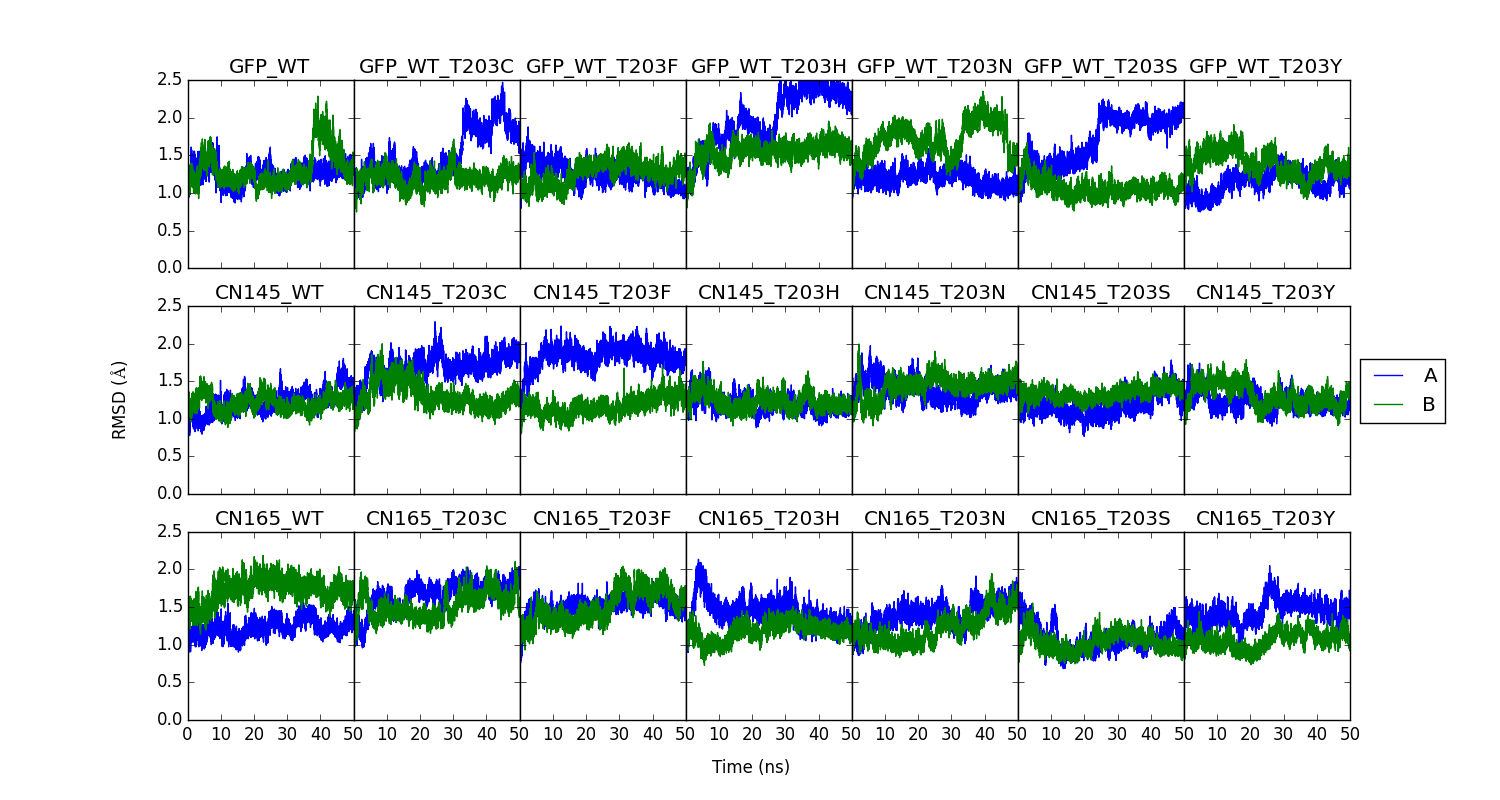
\includegraphics[width=\double]{figures-gfp-pKa/combined_rmsd.png}
    \caption[RMS deviations of each GFP construct]{
       RMS deviations as a function of MD simulation time relative to the initial minimized starting structure of the 21 GFP mutants containing the fluorophore in the A state (blue) and B state (green).
   }
    \label{fig:rmsd}
\end{figure}

Using these trajectories, we performed \pKa{} calculations on an ensemble of structures extracted at regular intervals from the MD simulations.
The first 10 \si{\ns} of each simulation were discarded as equilibration time, and an ensemble of 80 structures, each 500 ps apart, were used to calculate an ensemble average of fluorophore \pKa{} values.
For all MD simulations and \pKa{} calculations, we observed convergence of the $\Delta G$ values (and thus the predicted \pKa{}) over the course of 50 \si{\ns} (Figure \ref{fig:dG_1stD}).
We therefore determined that additional simulation time would not result in changes in the calculated \pKa{} values. 

\begin{figure}
    \center
    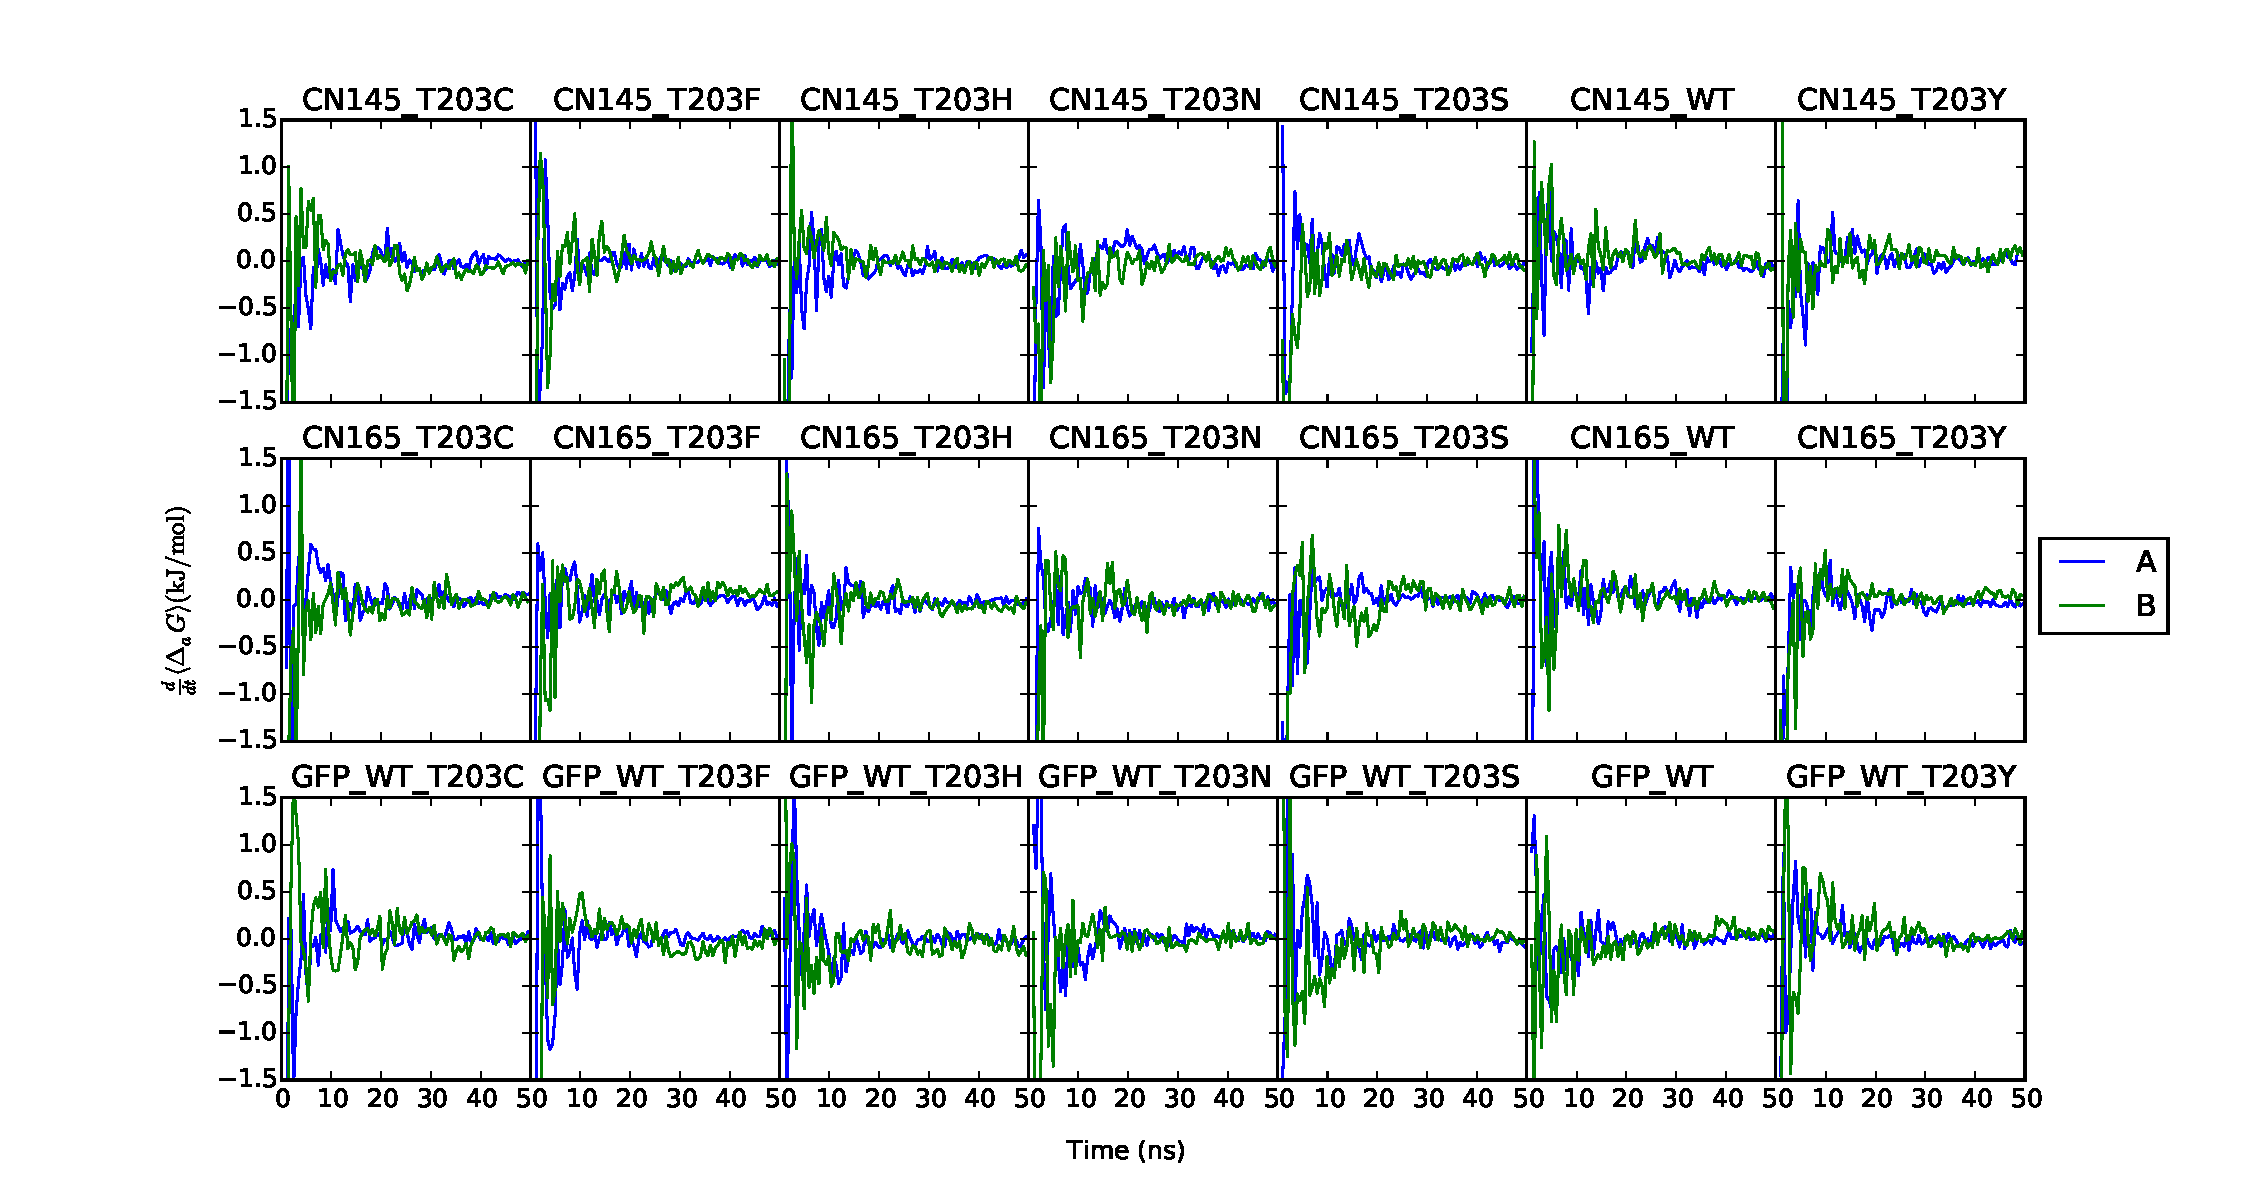
\includegraphics[width=\double]{figures-gfp-pKa/dG_firstDerivative.pdf}
    \caption[Convergence of $\Delta G$ calculations]{
        First derivative of the calculated $\Delta G$ for the A (blue) and B (green) states over 50 ns of MD simulation for all 21 GFP mutants. 
        Labels CN145 and CN165 designate the mutants with \pCNF{} at positions 145 and 165, respectively.
    }
    \label{fig:dG_1stD}
\end{figure}

We performed our \pKa{} calculations on each extracted frame and where we explicitly included any water molecules within a 5 \si{\angstrom} sphere of the phenolic oxygen of the fluorophore.
The explicit atoms (protein and water) were treated with a dielectric of 6, and any waters outside of this sphere were removed and replaced with a continuum dielectric of 78.54.
Thus, our calculations were insensitive to the location of origin of any particular water molecules, because they were allowed to move into and out of the 5 \si{\angstrom} sphere throughout the MD simulation.
The reduction of the dielectric constant to 6 for the explicit atom region (as opposed to 20 in the static structure calculation) accounts for the inclusion of protein dynamics in the model.
The results of these calculations are shown in Figure \ref{fig:calc_pKas}B, where we still observed a poor correlation to the experimental values ($r = 0.48$).
We explored the effect of different dielectric constants (between 2-8) for the explicit atom region, and observed that the value of the protein dielectric constant did not substantially affect the correlation to experiment (data not shown).
We decided 6 was the most appropriate dielectric constant for these calculations, as it best recreated a one-to-one correlation to the experimental \pKa{} values, and could account for the polarizability and other electronic properties of the protein.

The results of these calculations are shown in Figure \ref{fig:calc_pKas}B, where we observed still a poor correlation to the experimental values ($r = 0.48$).
Overall, our results suggest that simple continuum models, such as the one used here, are inadequate to describe the electrostatic heterogeneity of the interior of GFP.
Additionally, even when combined with expensive all-atom simulations with explicit water, the correlation to experiment does not significantly improve.
One potential shortcoming of this calculation method is that we have ignored any coupling between the titration states of the fluorophore and the surrounding titratable residues (most notably E222 and H148).
While there is indirect crystal structure evidence\cite{Elsliger1999} that E222 remains protonated in both the A and B states of the fluorophore, this may not necessarily hold true for all the mutants we investigated.
Further studies are underway to explore the effects of different spheres of inclusion of explicit waters,  and using different dielectric constants of protein, and titration state coupling between the fluorophore, E222, and H148.

Despite the inability of APBS to accurately reproduce these experimentally measured \pKa{} values, our data set is unique and offers benefits over current protein electrostatics benchmarks.
Here, we have made systematic mutations at a single site (position 203) near the same titration event (GFP fluorophore) that result in \pKa{} changes of nearly 2 pH units.
This is in contrast to traditional data sets of \pKa{} values measured at various sites throughout the entirety of globular proteins like \emph{Staphylococcal} nuclease or lysozyme \cite{Nielsen2011, Castaneda2009, Merz1991}.
While these traditional data sets allow for rigorous tests of \pKa{} prediction models, they are comprised of titratable residues that exist in environments that are drastically different in both solvent and protein environment, making it difficult to identify the causes of success and failure in \pKa{} predictions.
The systematic nature of these \pKa{} shifts in the unique, water-filled \textbeta{}-barrel of GFP could offer a convenient alternative benchmark. 

\subsection{Calculating Nitrile Electric Fields}

For 14 of these protein systems, a \pCNF{} residue at either position 145 or 165 was used as a VSE reporter of electric field change based on Equation \ref{eq:stark}.
Because site-specific electric fields, specifically those projected along the nitrile bond axis of \pCNF{} 145 and 165, are easily accessible from our MD simulations, we wanted to test whether the absolute values of the measured nitrile frequencies were correlated to these calculated fields.
We chose to calculate the fields using the Reaction Field method, which has been described in detail elsewhere and is known to minimize the error implicit in integrating the PB equation (eq \ref{eq:PB}) \cite{Ritchie2015}.
We performed the APBS electric field calculations on 80 frames collected every 500 ps from our all-atom, explicitly-solvated protein trajectories.
In accordance with the RF method, the protein was treated with a dielectric constant of 2 and all waters (except those within a 5 \si{\angstrom} sphere of the \pCNF{} probe) were replaced with a dielectric constant of 78.54.
Additionally, because we simulated the A and B states separately for each mutant, and the experimental frequencies were measured for proteins that exist in an equilibrium of A and B states, it was necessary to weight the trajectories in order to calculate fields which were consistent with our VSE measurements.
For all of the simulations, the average field converged to a single value during the course of the simulation (Figure \ref{fig:force_1stD}).
Here, we report a weighted average of the A and B state fields at the midpoint of the nitrile bond, where the weights were assigned based on the experimental \pKa{} values and the Henderson-Hasselbalch equation.
The individual fields for the A and B state of each mutant are shown in Table \ref{tbl:ind_forces}, where we generally observed small differences in fields between the A and B state simulations compared to the size of electric field fluctuations.
The results of these field calculations are plotted against the experimental vibrational frequencies (determined from Figure \ref{fig:abs_spectra}D) in Figures \ref{fig:calc_forces}A,B.
In both the case of the \pCNF{} 145 and 165 probes, the continuum based model again failed to describe the complex interior of GFP, with correlations to experiment of -0.05 and 0.41, respectively.
To test the sensitivity of these calculations to the salt concentration within the simulation box, we performed calculations with 12 and 24 additional sodium and chloride ions.
However, even at high salt concentrations, the calculated fields at the nitrile bond did not significantly change (data not shown).
We believe that a model that can accurately describe the polarity and polarizability of, as well as the specific hydrogen bonding interactions inside, GFP will be necessary to accurately reproduce these experimentally measured nitrile frequencies \cite{Blasiak2016}.
We are currently expanding our studies of these nitrile probes to locations other than 145 and 165 to test the general applicability of these continuum-based models to reproduce the measured nitrile frequencies.

\begin{figure}
    \center
    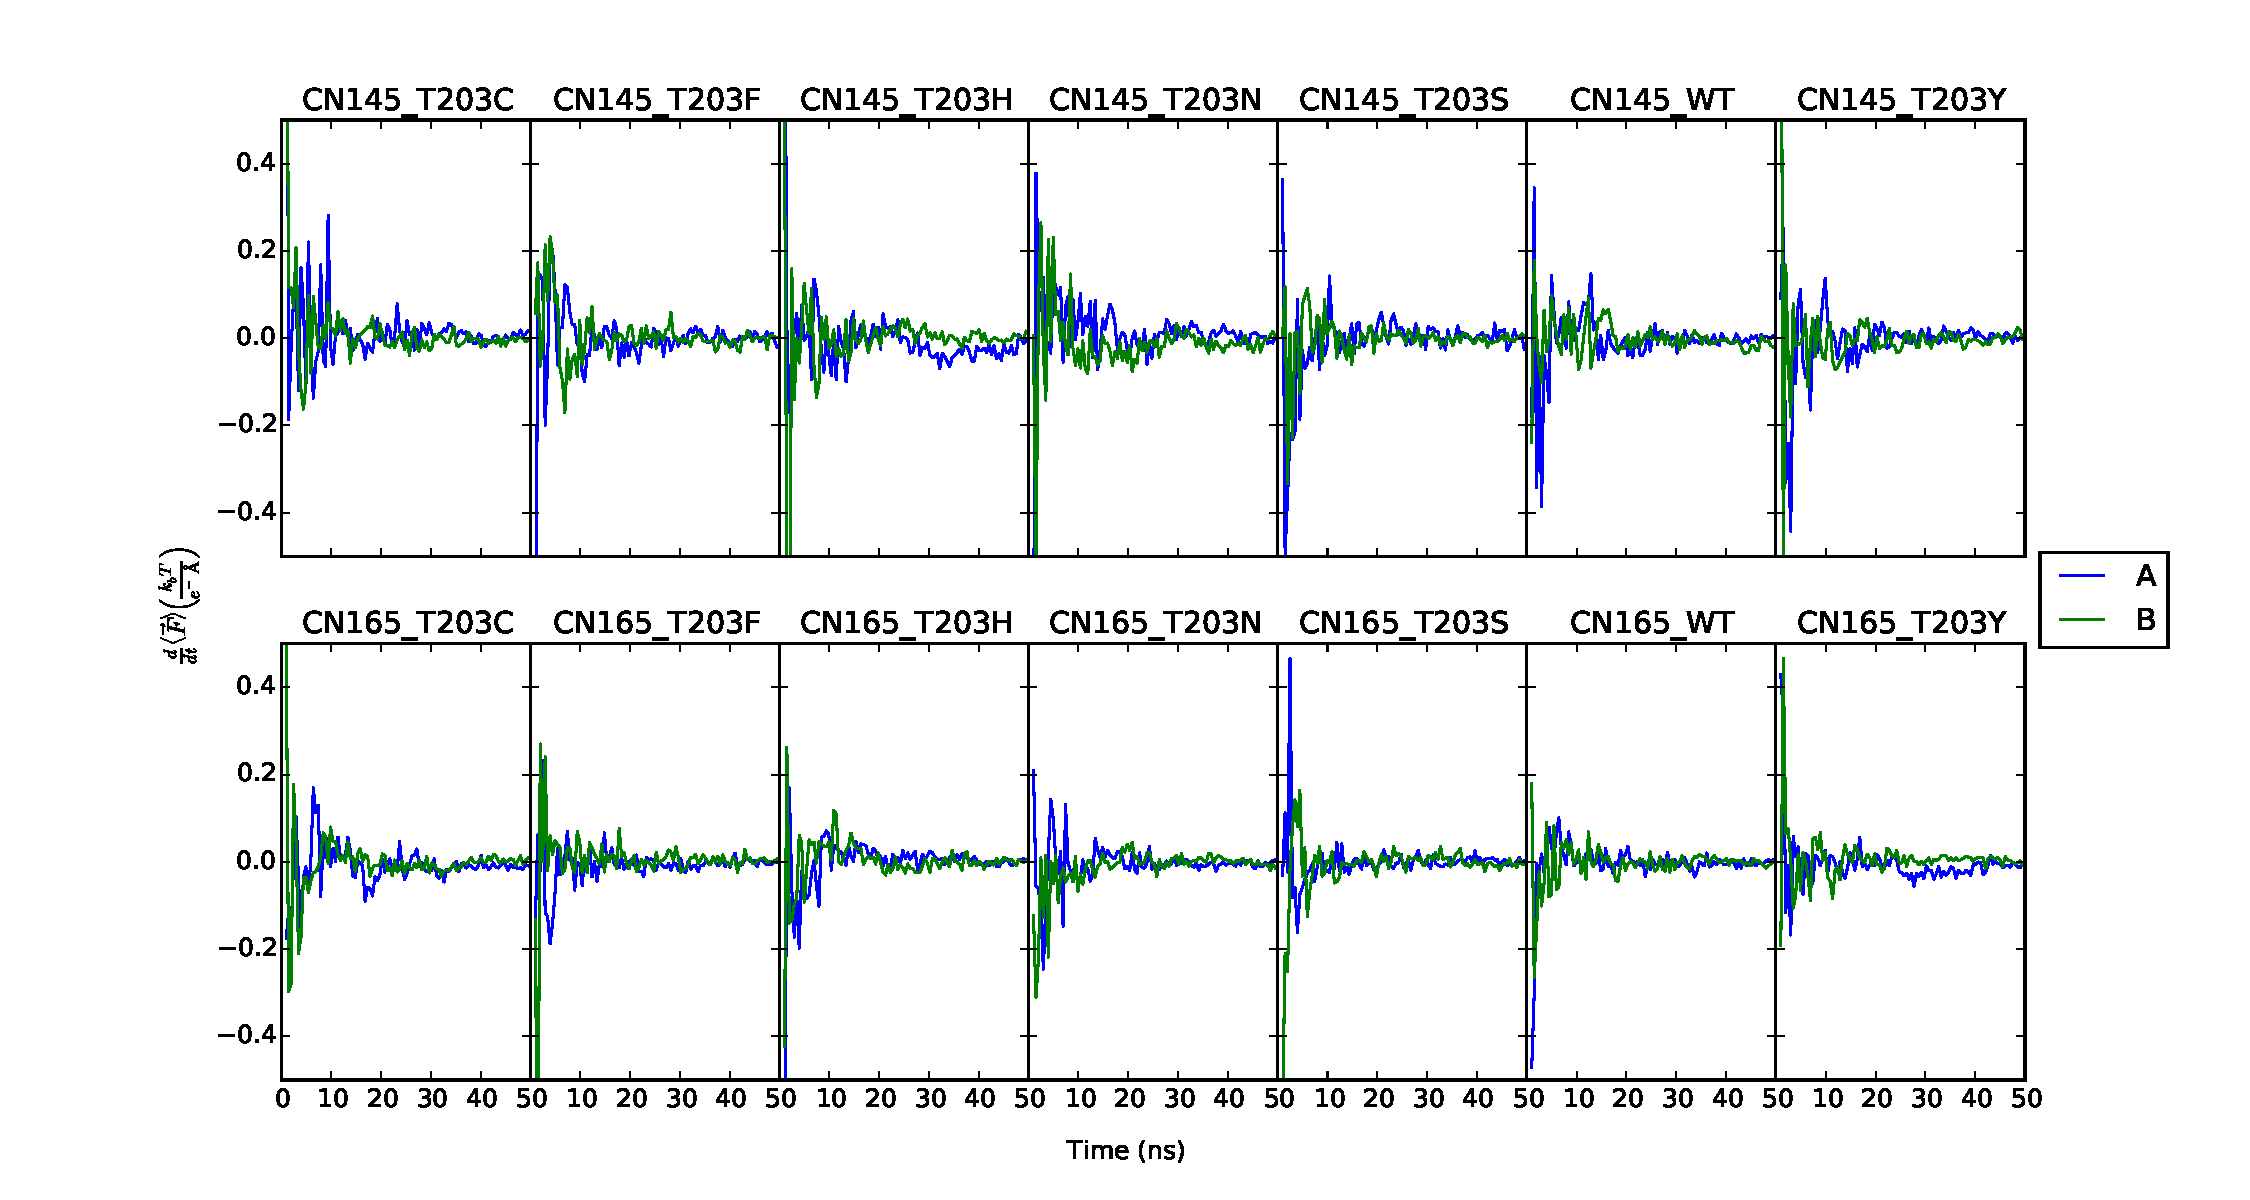
\includegraphics[width=\double]{figures-gfp-pKa/force_APBS_firstDerivative.pdf}
    \caption[Convergence of force calculations]{
        First derivative of the calculated force at the midpoint of the nitrile for the A (blue) and B (green) states over 50 ns of MD simulation for all 14 nitrile-containing GFP mutants. 
        Labels CN145 and CN165 designate the mutants with \pCNF{} at positions 145 and 165, respectively.
    }
    \label{fig:force_1stD}
\end{figure}

\begin{table}
    \caption[Calculated fields experienced by the nitrile in each fluorophore state]{
        Ensemble averaged electric fields (in MV/cm) experienced by the nitrile probes with the GFP fluorophore in either the A or B state.
    }
    \begin{center}
    \begin{tabular}{ll| cccc}
    \toprule
    Nitrile & 203 Mutation & $\left < \vec{F} \right >_A $ & $\left < \vec{F} \right >_B $ & Weighted & STD \\
    \toprule
    \multirow{6}{*}{CN145}
     & T203C  & -18.0 & -27.2 & -20.3 & 20.5 \\
     & T203F  & -31.5 & -33.8 & -32.9 & 20.7 \\
     & T203H  & -34.0 & -26.6 & -27.1 & 56.8 \\
     & T203N  & -25.0 & -38.3 & -33.0 & 22.4 \\
     & T203S  & -26.7 & -26.7 & -26.7 & 23.5 \\
     & T203Y  & -26.8 & -32.7 & -28.1 & 22.2 \\
     & WT     & -29.9 & -29.6 & -29.6 & 30.0 \\
    \midrule
    \multirow{6}{*}{CN165}
     & T203C  & -7.5  & -6.9  & -7.3  & 19.9 \\
     & T203F  & -7.0  & -3.2  & -5.3  & 20.2 \\
     & T203H  & -2.7  & -9.0  & -7.8  & 20.8 \\
     & T203N  & -2.4  & -11.5 & -6.8  & 16.8 \\
     & T203S  & -6.4  & -2.9  & -3.5  & 24.0 \\
     & T203Y  & -6.9  & -7.8  & -7.1  & 25.2 \\
     & WT     & -11.8 & -3.8  & -6.8  & 18.6 \\
    \bottomrule

    \end{tabular}
    \end{center}
    \label{tbl:ind_forces}
\end{table}

\begin{figure}
    \center
    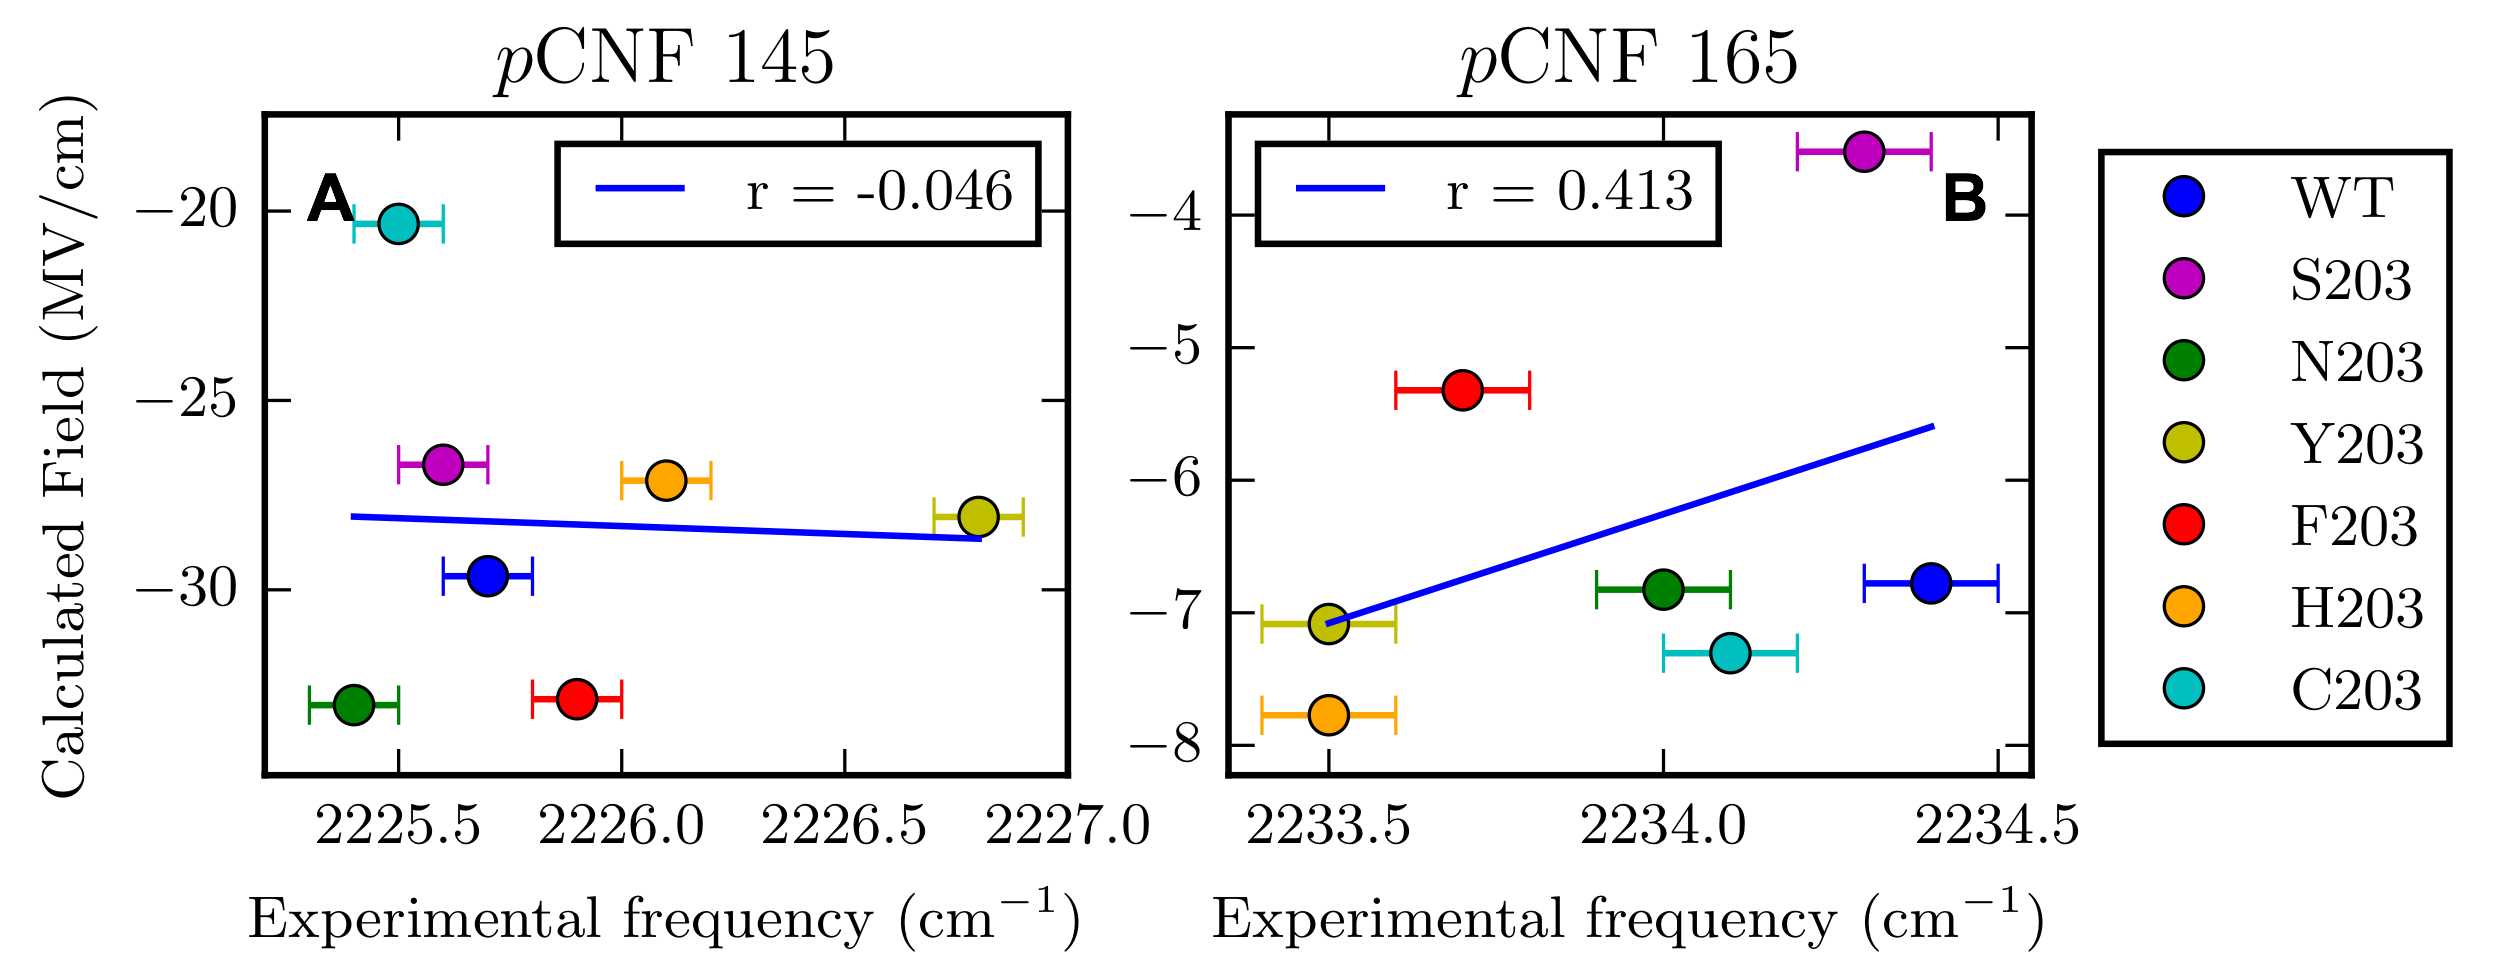
\includegraphics[width=\double]{figures-gfp-pKa/calc_forces.png}
    \caption[Comparison of calculated fields against experimental frequencies]{
        Comparison of the experimentally measured nitrile frequencies to calculated electric fields along the nitrile bond of \pCNF{} 145 and 165. 
        Error bars on the $y$-axis have been omitted for clarity; 
        in general, the distributions of fields calculated for each data point from the ensemble of MD structures are large relative to the shifts in average field ($\pm100\%$). 
        (A) Calculated field using the APBS-based RF method along the bond vector of \pCNF{} 145 compared to the experimentally measured vibrational frequency. 
        (B) Calculated field using the APBS-based RF method along the bond vector of \pCNF{} 165 compared to the experimentally measured vibrational frequency.
    }
    \label{fig:calc_forces}
\end{figure}

%%%%%%%%%%%%%%%%%%%%%%%%%%%%%%%%%%%%%%%%%%%%%%%%%%%%%%%%%%%%%%%%
%%%%%%%%%%%%%%%%%%%%%%%%%%%%%%%%%%%%%%%%%%%%%%%%%%%%%%%%%%%%%%%%
\section{Conclusions}\label{pKa-conclusion}
%%%%%%%%%%%%%%%%%%%%%%%%%%%%%%%%%%%%%%%%%%%%%%%%%%%%%%%%%%%%%%%%
%%%%%%%%%%%%%%%%%%%%%%%%%%%%%%%%%%%%%%%%%%%%%%%%%%%%%%%%%%%%%%%%


Here, we have shown that shifts in GFP fluorophore \pKa{} caused by nearby amino acid mutations are generally in good agreement with the corresponding Stark effect shifts of both the fluorophore and \pCNF{} probes inserted near the fluorophore.
This observed agreement between the vibrational and electronic Stark effect probes and \pKa{} shifts not only provides confidence in each of these measurements as probes of non-covalent environment, but also offers an unprecedented level of information about the electrostatic environment around the GFP fluorophore.
Because of this, we think the GFP fluorophore offers a unique benchmark for electrostatics models.
Contrary to datasets of \pKa{} values measured from titratable residues at various sites in the interior of a protein, we have measured \pKa{} shifts of a single interior site as a function of changes in local environment, caused by the position 203 mutations.
In addition to providing a range of \pKa{} values of the same residue as a function of nearby mutations, this dataset also offers the ability to benchmark electrostatics models against site-specific measurements of electric field changes that arise from the same mutations.
To test these possibilities, we used the popular APBS software package, coupled with MD simulations, to calculate the fluorophore \pKa{} values and the site-specific electric fields experienced by the nitrile probes.
We found that the continuum treatment of the GFP interior is insufficient to accurately reproduce the experimentally measured \pKa{} values and electric fields shifts.
In summary, we have reported that electrostatic perturbations, induced by mutations at position 203, cause similar changes in (1) the VSE shifts of inserted nitrile probes; (2) the electronic Stark effect shifts of the GFP fluorophore; and (3) the fluorophore \pKa{} values.
We suggest that the data presented here will be useful to other researchers, not only to validate protein electrostatic models, but also to elucidate the underlying physical determinants of fluorophore equilibrium in fluorescent proteins. 


\chapter{Quantifying the Effects of Hydrogen Bonding on Nitrile Frequencies in GFP: Beyond Solvent Exposure}\label{gfp-hbond}

Vibrational spectroscopy is a powerful tool for characterizing the complex non-covalent interactions that arise in biological systems.
The nitrile stretching frequency has proven to be a particularly convenient biological probe, but the interpretation of the spectra of nitriles is complicated by their sensitivity to local hydrogen bonding interactions.
This often inhibits the straightforward interpretation of nitrile spectra by requiring knowledge of the molecular level details of the local environment surrounding the nitrile.
While the effect of hydrogen bonds on nitrile frequencies has been well documented for small nitriles in solution, there have been relatively few studies of these effects in a complex protein system.
Therefore, we introduced a nitrile probe at nine locations throughout green fluorescent protein (GFP) and compared the mean vibrational frequency of each probe to the specific hydrogen bonding geometries observed in molecular dynamics (MD) simulations.
We show that a continuum of hydrogen bonding angles is found depending on the particular location of each nitrile, and that the differences in these angles account for the differences in the measured nitrile frequency.
We further observed that the temperature dependence of the nitrile frequencies (measured as a frequency-temperature line slope, FTLS) was a good indicator of the hydrogen bonding interactions of the probe, even in scenarios where the nitrile was involved in complex and restricted hydrogen bonds, both from protein and from water.
While constant offsets to the nitrile frequency to all hydrogen bonding environments have been applied before to interpret shifts in nitrile frequency, we show that this is insufficient in systems where the hydrogen bonds may be restricted by the surrounding medium.
However, the strength of the observed correlation between nitrile frequency and hydrogen bonding angle suggests that it may be possible to disentangle electrostatic effects and effects of the orientation of hydrogen bonding on the nitrile stretching frequency.
Meanwhile, the experimental measurement of the FTLS of the nitrile is an excellent tool to identify changes in the hydrogen bonding interactions for a particular probe.

%%%%%%%%%%%%%%%%%%%%%%%%%%%%%%%%%%%%%%%%%%%%%%%%%%%%%%%%%%%%%%%%
%%%%%%%%%%%%%%%%%%%%%%%%%%%%%%%%%%%%%%%%%%%%%%%%%%%%%%%%%%%%%%%%
\section{Introduction}\index{hbond-intro}
%%%%%%%%%%%%%%%%%%%%%%%%%%%%%%%%%%%%%%%%%%%%%%%%%%%%%%%%%%%%%%%%
%%%%%%%%%%%%%%%%%%%%%%%%%%%%%%%%%%%%%%%%%%%%%%%%%%%%%%%%%%%%%%%%

The complex networks of non-covalent interactions that arise from the arrangement of thousands of partially charged atoms in biological molecules are responsible for many important biomolecular functions, including protein folding, protein-protein interactions, membrane fluidity and permeation, ligand binding, signaling pathways, and catalysis \cite{Honig1995}.
Characterizing and understanding the molecular details of the environments that give rise to biological function is of critical importance to modern biophysics.
The inherent spatial and temporal resolution of molecular vibrations have been exploited by many researchers to directly probe biological systems.
Specifically, the nitrile stretching frequency has been widely used as a probe of site-specific dynamics \cite{Fang2008, Sigala2007, Yoshikawa1985}, hydration \cite{Waegele2009, Oh2008}, and electric fields\cite{Webb2008, Slocum2016, Shrestha2015, Shrestha2017, Andrews2000, Andrews2002} in a variety of biological systems due to its extraordinary environmental sensitivity.
Nitrile vibrational probes absorb in a relatively transparent region of the infrared spectrum, have reasonable oscillator strengths \cite{Webb2008}, and can be easily incorporated through a variety of synthetic and biosynthetic methods\cite{Fafarman2006, Getahun2003, Kirshenbaum2002} to interrogate DNA, proteins, and membranes. 

Despite the widespread use of nitriles as biomolecular probes and the relative ease with which their frequencies can be measured in a variety of applications, it is not trivial to meaningfully interpret a measured nitrile frequency in a complex biological system.
This is largely due to the convolution of the competing effects of Coulombic frequency shifts, commonly referred to as the vibrational Stark effect (VSE), and frequency shifts due to specific interactions such as hydrogen bonding.
While the effects of solvent electric field and specific hydrogen bonding interactions on nitrile frequencies have been well characterized for small nitriles in solution \cite{Levinson2012, Blasiak2017, Deb2016}, the theoretical basis for these convoluted effects does not always successfully translate to the interpretation of nitrile frequencies in more complex systems like a solvated protein.
Indeed, the ability to interpret nitrile frequencies in terms of electric fields via a VSE analysis when the nitrile experiences hydrogen bonds has been under question for quite some time \cite{Slocum2016, Fafarman2010, Bagchi2012, Slocum2018}.
While it is clear that VSE analyses of nitrile frequencies can be used to quantify relative electric fields between nitriles that are engaged in similar hydrogen bonding interactions \cite{Slocum2016}, there is still debate on how to define criteria that must be met in order for two nitriles to be classified within this regime.
This is further complicated by a lack of experimental methodologies to specifically test \emph{in situ} if these hydrogen bonding criteria are met.
Conversely, the use of nitrile frequencies as site-specific probes of solvent exposure inherently ignores any electrostatic contribution to the frequency by equating blue shifted spectra with solvent exposed locations and red shifted spectra with buried locations.
The possibility that electric field effects would red-shift the spectrum of a solvent exposed nitrile or blue-shift the spectrum of a buried nitrile is usually not considered.

Significant theoretical effort has been made towards developing quantitative models that can capture the competing effects of hydrogen bonding and Coulombic forces on nitrile frequencies.
Early theories focused on relating bulk properties of the solvent to the nitrile frequency \cite{Kirkwood1934, Onsager1936}.
While these theories have worked well for aprotic solvents, it has become increasingly apparent that specific molecular interactions between the nitrile and the surrounding solvent are a major contributor to the nitrile frequency in environments rich in hydrogen bond donors, such as aqueous solvent or a protein interior \cite{Blasiak2017}.
Recently, B\l{}asiak et al. developed a highly quantitative model based on combined quantum mechanical (QM) methods and molecular dynamics (MD) simulations that accurately captured the direction of nitrile frequency shifts in different solvent environments \cite{Blasiak2016}.
However, these models are computationally expensive and it is therefore useful to develop a nitrile classification system based strictly on geometric parameters of hydrogen bonding interactions that can be determined from MD simulations as a complement to rigorous QM modeling.


Using \emph{ab initio} calculations of clusters of water hydrogen bound to both acetonitrile and methyl thiocyanate, Choi et al. observed that in linear $\sigma$-hydrogen bonds the nitrile bond was shortened, leading to an increase in the nitrile stretching frequency.
However, at the small angles found in $\pi$-hydrogen bonds, the nitrile bond was lengthened leading to a decrease in electron density and a decrease in the nitrile frequency \cite{Choi2008}.
Fafarman et al. showed that vibrational frequencies of nitriles involved in unrestricted hydrogen bonds can be deconvoluted into electrostatic effects and hydrogen bonding effects by comparing nitrile frequencies to an independent $^{13}$C NMR parameter \cite{Fafarman2010}.
For nitriles that were well exposed to water, the authors observed a constant vibrational absorption shift of 10 \si{\wn} relative to the observed NMR chemical shift, which was in good agreement with the calculated frequencies for linear hydrogen bonds.
However, in the confined environment of the interior of a protein, steric interactions often enforce non-linear hydrogen bonding geometries.
While these issues have been examined theoretically, there has not been an experimental study on the effects of hydrogen bonding on nitrile frequencies in such cases.

Our laboratory has been particularly interested in experiments that can disentangle the contributions of hydrogen bonding from other influences on the nitrile vibrational frequency, such as those from the VSE.
Measurement of the temperature dependence of the nitrile absorption frequency has been useful in this regard.
In 2003, Getahun et al. first reported the linear temperature dependence of the nitrile stretching frequencies of nitrile-substituted amino acids, with anomalous narrowing of the absorption spectrum with increasing temperature \cite{Getahun2003}.
This observation inspired the use of the nitrile as a probe in conformational or unfolding studies initiated with a temperature jump \cite{Getahun2003, Huang2003}.
In 2007, Maienschein-Cline and Londergan used the temperature dependence of the nitrile frequency to demonstrate that the nitriles were also probes of local hydrogen bonding and solvent dynamics \cite{Maienschein-Cline2007}.
In 2012, Fafarman and Boxer used the temperature dependence of a nitrile to distinguish between two subpopulations of the spectrum of a nitrile in a protein \cite{Fafarman2010a}.
Finally, in 2015, Adhikary et al. postulated that the temperature dependence of the nitrile absorption measured via the frequency-temperature line slope (FTLS) was related to the hydrogen bonding environment experienced by small nitriles in various solvents and in proteins, and the authors were able to use the nitrile FTLS to assess whether or not a particular location was buried or solvent exposed \cite{Adhikary2015}.

While nitrile frequencies have clearly been useful in determining site-specific solvent exposure in proteins, it is often overlooked that solvent exposure is not a binary state, in which the nitrile is either solvent exposed or buried.
While locations on a protein surface might have a relatively constant extent of solvation, locations within a protein can experience a near continuous range of solvent exposure depending on microscopic details of the steric and electrostatic landscape at any given location in the protein's 3D structure.
Moreover, the hydrogen bond strength and geometry may change continuously based on the dynamics of the protein and the solvent.
In this study, we examine these effects using green fluorescent protein (GFP) as a model system.
The water filled $\beta$-barrel of GFP provides a range of different hydrogen bonding profiles because the complex network of confined water on the interior of the protein is stabilized by hydrogen bonds to other waters and nearby protein residues and varies in allowed hydrogen bonding geometries, rates of diffusion, and interaction strength.
Each of these different hydrogen bonding environments could contribute to a frequency shift of differing magnitude in a way not described by the VSE.
Here, we use a combination of FTLS measurements and MD simulations to show that the FTLS is related to small differences in hydrogen bonding profiles and is therefore useful beyond just the Boolean classification of a nitrile as either engaging in hydrogen bonding or free from hydrogen bonding.
Instead, the FTLS can be used to differentiate a range of solvent exposure and even differences in specific hydrogen bonding angles.
This makes the FTLS a powerful diagnostic tool for interpreting any nitrile spectrum, as it allows for the rapid comparison of hydrogen bonding interactions of different states.
In the context of a VSE experiment, the FTLS could confirm that the hydrogen bonding interactions have not changed from the reference to perturbed state. 

To evaluate the FTLS of nitriles as a diagnostic tool of hydrogen bonding environment, we biosynthetically incorporated \emph{p}-cyanophenylalanine (CNF) at nine locations in GFP.
The locations were chosen based on the PDB crystal structure 2b3p\cite{Pedelacq2006} to sample a broad range of solvent accessibility and hydrogen bonding environments.
Using the crystal structure, we classified \emph{a priori} the locations as solvent exposed or buried based on the crude assessment of whether or not the side chain was pointed into the interior of the $\beta$-barrel.
The nine locations chosen are shown in Figure \ref{fig:hbond-system}, where the colored spheres indicate a residue that was independently mutated to CNF.
We collected temperature dependent Fourier transform infrared (FTIR) spectra and performed MD simulations of each nitrile-containing protein variant.
We found that there is a strong correlation between the FTLS and the solvent accessible surface area (SASA) of the CNF residue (determined from MD simulations) despite the diverse hydrogen bonding profiles.
This indicates that the FTLS can be used reliably and rapidly to test differences in hydrogen bonding interactions of nitrile probes.
Additionally, we compared the measured stretching frequencies of nitriles involved in various restricted hydrogen bonding orientations (again determined from MD simulations) to the effects predicted by changes in the angle of the hydrogen bond to the nitrile.
We found that the observed vibrational shifts of the nitrile in each location can be attributed almost entirely to the average orientation of hydrogen bonds experienced by the nitrile.
Although acetonitrile and CNF are structurally different, we expect them to behave similarly in this regard, as they have been shown to respond similarly to other spectroscopic perturbations \cite{Getahun2003}.
This observation confirms the predictions by Choi et al. and underlines the importance of understanding the molecular-level details of the hydrogen bonding interactions to the nitrile  before interpreting its vibrational spectrum.

\begin{figure}
    \center
    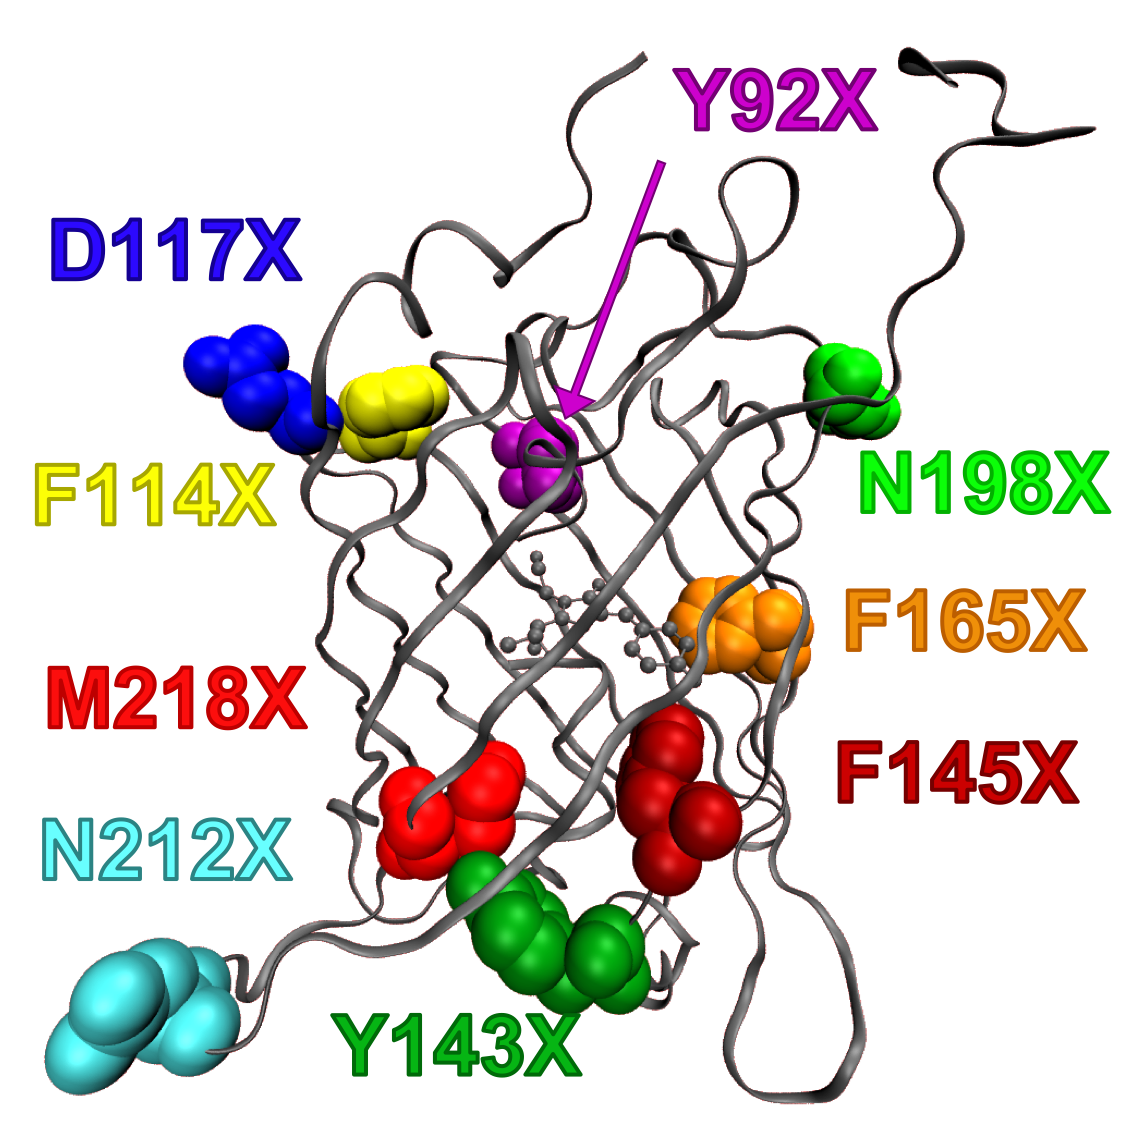
\includegraphics[width=3.25in]{figures-gfp-hbond/system.png}
    \caption{Locations of the nitrile probes in green fluorescent protein (GFP) shown on the crystal structure 2b3p. Each location shown in the spherical representations was independently mutated to \emph{p}-cyanophenylalanine (CNF). The first letter indicates the one-letter amino acid code of the residue that was replaced by CNF, denoted by ``X''.}
    \label{fig:hbond-system}
\end{figure}

%%%%%%%%%%%%%%%%%%%%%%%%%%%%%%%%%%%%%%%%%%%%%%%%%%%%%%%%%%%%%%%%
%%%%%%%%%%%%%%%%%%%%%%%%%%%%%%%%%%%%%%%%%%%%%%%%%%%%%%%%%%%%%%%%
\section{Methods}\index{hbond-methods}
%%%%%%%%%%%%%%%%%%%%%%%%%%%%%%%%%%%%%%%%%%%%%%%%%%%%%%%%%%%%%%%%
%%%%%%%%%%%%%%%%%%%%%%%%%%%%%%%%%%%%%%%%%%%%%%%%%%%%%%%%%%%%%%%%

\subsection{Protein Expression and Purification}

A pBAD vector containing the gene for 6xHis-tagged superfolder GFP (Addgene plasmid \#85482) and a pDule vector containing a tRNA synthetase/tRNA pair evolved for CNF (Addgene plasmid \#85494) were kindly provided by the Mehl group \cite{Miyake-Stoner2009, Miyake-Stoner2010}.
Amber codons were introduced into the superfolder GFP (hereafter, simply GFP) gene at the desired locations, and the amber-coded pBAD vector was co-transformed alongside the pDule vector into DH10$\beta$ cells.
Single colonies from plates containing ampicillin and tetracycline were used to seed the growth of 1 L cultures in an autoinduction media described by Mehl et al \cite{Hammill2007}.
After 24-30 h of expression, cells were harvested and either purified immediately or stored at -80 \si{\celsius} until further use.
6xHis-tagged GFP mutants containing CNF were purified by immobilized metal affinity chromatography, and the 6xHis tags were cleaved with trypsin proteolysis.
Cleaved GFP mutants were buffer exchanged into degassed phosphate buffered saline (PBS) at pH 7.4 and used immediately or stored at -80 \si{\celsius}. 

\subsection{FTIR Spectroscopy}

Nitrile-containing GFP mutants were concentrated to $\sim$2 mM using Amicon Ultra 10 000 molecular weight cutoff filters according to the manufacturer's protocol.
Following concentration, samples were spun for 5 minutes at 15 000 rpm to remove any air bubbles.
Samples were injected into a temperature-controlled cell at 5 \si{\celsius} between two sapphire windows separated by two 100 $\mu$m teflon spacers.
Spectra were recorded at 5, 15, 25, and 35 \si{\celsius}, in that order, averaging over 600 scans at a resolution of 0.5 \si{\wn}, allowing the sample to equilibrate for at least 10 minutes before scanning at each temperature.
At the end of the 35 \si{\celsius} measurement, the intact cell was cleaned with water and ethanol, and then PBS was added to the 35 \si{\celsius} equilibrated cell for background spectra, which were collected in the reverse order of temperature to avoid the formation of air bubbles during the scans.

\subsection{Molecular Dynamics Simulations}

A template protein was modeled by homology from the 2b3p crystal structure\cite{Pedelacq2006} using a procedure described elsewhere \cite{Slocum2017}.
Using this template, nine separate mutations from the WT residue to phenylalanine were made using the mutagenesis wizard tool in PyMol\cite{DeLano2002} at each of the CNF locations.
Using the Avogadro molecular editing package \cite{Hanwell2012}, the mutated phenylalanine residue was further modified to CNF and independently minimized.
Parameters for the internal GFP fluorophore were kindly provided by Riccardo Nifos\'i \cite{Nifosi2003}, and parameters for the CNF chromophore have been described previously \cite{Slocum2017}.
All further minimizations and MD simulations were performed using the Gromacs 5.0.4 molecular dynamics simulation package \cite{VanDerSpoel2005, Abraham2015}, and the Amber03 force field (ffAmber03) \cite{Duan2003, Sorin2005}. 

Each of the nine protein systems was energy minimized in vacuum using the steepest descent algorithm and then solvated in a dodecahedron box of TIP3P water \cite{Jorgensen1983}, with a minimum distance of protein to the edge of the box of 1.5 nm.
The solvated systems were then energy minimized using a steepest descent approach, and then heated under the NVT ensemble at 300 K, and equilibrated under the NPT ensemble at 1 atm.
Production MD was run on each equilibrated protein system for 50 ns, using the same simulation parameters as described previously \cite{Slocum2017}, and a snapshot was saved every 4 ps.
The first 10 ns was discarded as equilibration time, and only the last 40 ns was used in the analyses that follow.

%%%%%%%%%%%%%%%%%%%%%%%%%%%%%%%%%%%%%%%%%%%%%%%%%%%%%%%%%%%%%%%%
%%%%%%%%%%%%%%%%%%%%%%%%%%%%%%%%%%%%%%%%%%%%%%%%%%%%%%%%%%%%%%%%
\section{Results}\index{hbond-results}
%%%%%%%%%%%%%%%%%%%%%%%%%%%%%%%%%%%%%%%%%%%%%%%%%%%%%%%%%%%%%%%%
%%%%%%%%%%%%%%%%%%%%%%%%%%%%%%%%%%%%%%%%%%%%%%%%%%%%%%%%%%%%%%%%
\subsection{Vibrational Absorption Measurements}

We measured the nitrile stretching frequencies of biosynthetically incorporated CNF probes at nine positions in GFP, as well as CNF in water and \emph{p}-tolunitrile in THF.
The resulting spectra at 25 \si{\celsius} are shown in Figure \ref{fig:hbond-spectra}, where the number to the right of each spectrum indicates the position of the probe according to Figure \ref{fig:hbond-system}.
Each spectrum was fit to a gaussian curve using an in-house fitting program described elsewhere \cite{Ragain2012}.
The mean vibrational frequency and fwhm of each spectrum are found in the Supporting Information (Table S1).
Most of the probe locations (114, 117, 143, 198 and 212) had mean vibrational frequencies that were centered around the value of CNF in water ($\sim$2238 \si{\wn}).
These five probe locations also had similar peak widths (measured as fwhm) to that of CNF in water ($\sim$10 \si{\wn}).
Two probe locations (165 and 218) had mean vibrational frequencies that were shifted to lower frequencies ($\sim$2234 \si{\wn} and $\sim$2231 \si{\wn}, respectively), but were still blue-shifted relative to \emph{p}-tolunitrile in THF.
These two locations had narrower peak widths ($\sim$8 \si{\wn} and $\sim$7 \si{\wn}, respectively).
One probe location (145) had a mean vibrational frequency of $\sim$2225 \si{\wn} and had the narrowest peak width ($\sim$5 \si{\wn}), which is both lower in frequency and narrower than \emph{p}-tolunitrile in THF.
The final probe location (92) had a mean vibrational frequency higher (2243 \si{\wn}) than that of CNF in water and the largest peak width of 12 \si{\wn}.
The range of measured frequencies of the nitrile in these locations is larger than the range for the small CNF analogs in THF (2228 \si{\wn}) and water (2238 \si{\wn}), which are the two solvents commonly used to represent the extremes of potential solvent hydrogen bonding for CNF.
Clearly, the broad range of hydrogen bonding environments available within a complex protein system is not adequately recapitulated by the solvatochromism of small nitrile derivatives. 

\begin{figure}
    \center
    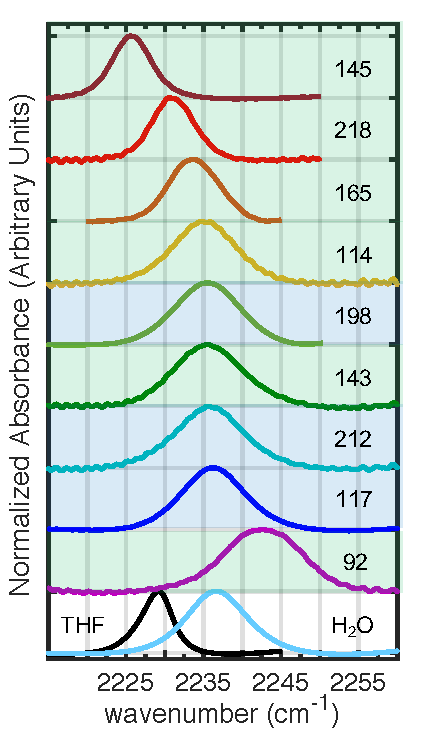
\includegraphics[width=3.00in]{figures-gfp-hbond/spectra_colors.pdf}
    \caption{Representative FTIR absorption spectra of CNF in each of the nine locations at 25 \si{\celsius}, arranged from the lowest to highest mean frequency. Each spectrum is normalized to a maximum absorbance of 1. The nitrile location for each spectrum is indicated by the number to the right, according to Figure \ref{fig:hbond-system}. The spectra are offset from the $x$-axis for clarity. The color of the background indicates our \emph{a priori} classification of the solvent accessibility of the nitrile location based on the crystal structure. Blue indicates a position where the wild type side chain is pointed away from the interior of the barrel, and thus the nitrile was expected to be solvent exposed. Green indicates a position where the wild type side chain is pointed into the interior of the barrel, and thus the nitrile was expected to be buried. At the bottom are representative spectra of \emph{p}-tolunitrile in THF at 25 \si{\celsius} (black) and CNF in water at 25 \si{\celsius} (light blue).}
    \label{fig:hbond-spectra}
\end{figure}

Next, we measured the temperature dependence of the nitrile stretching frequencies for each of the nine positions in GFP, as well as CNF in water and \emph{p}-tolunitrile in THF, over the range of 5-35 \si{\celsius}.
Over this temperature range, GFP has been shown be to remain stably folded \cite{Slocum2016, Pedelacq2006}.
The mean vibrational frequency and fwhm of each spectrum at each temperature are also found in the Supporting Information (Table S1).
Figure \ref{fig:hbond-ftls} shows the change in nitrile center frequency (relative to the frequency at 5 \si{\celsius}) as a function of temperature.
Similar to the work of Adhikary et al. \cite{Adhikary2015}, we measured a linear response over this temperature range for each of the probe locations, as well as for the small molecules.
For the aprotic solvent THF, we did not measure any change in the nitrile stretching frequency over this temperature range (Figure \ref{fig:hbond-ftls}, black).
Conversely, for CNF in water we measured a large change in frequency as a function of temperature (Figure \ref{fig:hbond-ftls}, light blue).
Interestingly, each nitrile location in our nine systems had a distinct FTLS, showing that our nine protein systems sampled a broad range of different hydrogen bonding interactions.
Most of the CNF probes in GFP gave temperature responses that were in between the extremes of THF and water, which suggests that these probes all experience varying amounts of hydrogen bonding that are not as strong as the well-solvated CNF in water.
However, for the nitriles at positions 212 and 92, we measured a FTLS greater than that for CNF in water, possibly suggesting that these two probe locations experience either more frequent, or stronger, hydrogen bonds than CNF in water.
This is not surprising for position 212, which is on a solvent exposed loop in GFP (Figure \ref{fig:hbond-system}).
However, position 92 is pointed into the GFP barrel, where we do not expect much interaction between the nitrile and water.
To interpret the differences in the FTLS of the nitrile in different locations, we turned to MD simulations to investigate the local hydrogen bonding interactions around each probe, including to the nitrile itself. 

\begin{figure}
    \center
    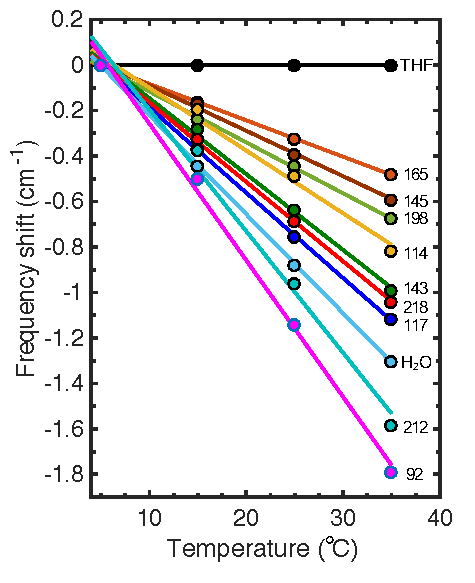
\includegraphics[width=3.25in]{figures-gfp-hbond/FTLS.pdf}
    \caption{Mean vibrational frequencies of CNF at each location as a function of temperature. The number to the right indicates the CNF location according to Figure \ref{fig:hbond-system}. Linear regression was used to fit a line to each data set. The slope of each trend line is the FTLS for that particular probe location. The temperature dependencies of the mean vibrational frequency of CNF in water (light blue) and \emph{p}-tolunitrile in THF (black) are also shown.}
    \label{fig:hbond-ftls}
\end{figure}

\subsection{SASA calculations}

In principle, the hydrogen bonding environment of a probe at any location could be investigated in a straightforward way through atomistic simulations.
One easy and popular choice for quantifying solvent exposure to specific residues within a protein is with the SASA of the amino acid.
However, SASA calculations suffer from the major disadvantage that they lack molecular details about solvent interactions.
Specifically, they do not include information about geometric orientations of hydrogen bonding, and they do not capture interactions that arise when a residue is not exposed to bulk solvent, such as those from confined waters or from the protein itself.
Nevertheless, SASA serves as a good first approximation to a measurement of hydrogen bonding interactions to the nitrile probe.  
Using the gmx sasa tool \cite{Eisenhaber1995}, we calculated the SASA of several subsets of the atoms within the CNF residue over the course of the 40 ns of production MD simulation for each GFP mutant. 
Specifically, we calculated the SASA of the nitrile alone, the nitrile plus the C$_{\beta}$, two H$_{\beta}$s and the phenyl ring, and the entire CNF residue including the backbone atoms.
The subsets for these calculations are illustrated in the Supporting Information (Figure S1), and the results are shown in Figure S2.
We found that the SASA of just the nitrile with its low total surface area was very sensitive to small changes in the surrounding protein structure, giving large fluctuations in SASA over the course of the simulation.
The SASA of the entire residue, shown in Figure \ref{fig:hbond-sasa}, gave the broadest range of values with the smallest standard deviations.
We have therefore chosen to focus on these values for the analysis that follows.
Across each of the nine CNF locations, there was a continuum of SASA possibilities ranging from completely solvent exposed to completely inaccessible.
SASA calculations revealed that two probes (positions 117 and 212) were highly solvent exposed and had SASAs that approached the calculated maximum of CNF by itself in solvent ($\sim$2.5 nm$^2$).
Three probes, at positions 114, 143 and 198, had intermediate SASAs ($\sim$0.5 nm$^2$ to 1.5 nm$^2$) relative to free CNF.
Two probes (positions 145 and 165) had a low SASA ($\sim$0.25 nm$^2$ to 0.5 nm$^2$) relative to free CNF.
Finally, two probes (positions 92 and 218) showed nearly zero SASA throughout the simulation, though these two had quite different FTLS values, shown in Figure \ref{fig:hbond-ftls}.
This discrepancy between the SASA and the measured FTLS suggests that the nitriles in these nine positions experienced differences in local environment more complex than could be captured by SASA calculations.

\begin{figure}
    \center
    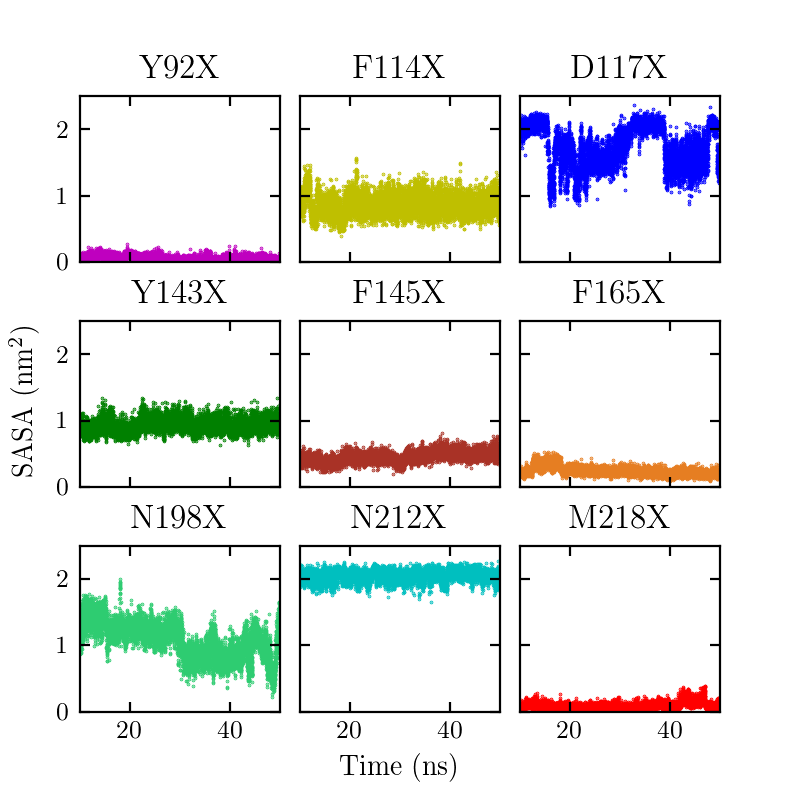
\includegraphics[width=3.25in]{figures-gfp-hbond/sasa_v_time.png}
    \caption{SASA of the CNF residue as a function of simulation time in 40 ns of production MD simulation for the nine GFP mutants containing the nitrile group.}
    \label{fig:hbond-sasa}
\end{figure}

\subsection{Hydrogen bonding calculations}

The MD simulations provide molecular level information about the hydrogen bonds around each nitrile probe that is significantly more detailed than the SASA.
For each of the nine systems, we analyzed the MD trajectories for the presence and geometry of hydrogen bonding using an in-house code to characterize hydrogen bonds to a nitrile probe in each frame of the simulation.
All nearby O, N, S, and C$_{\alpha}$ atoms were considered to be potential donors.
A hydrogen bond donor was determined to be hydrogen bonding if three conditions were satisfied: 1) the C--N$\cdots$H angle was greater than \ang{99} ($\theta_1$ in Figure \ref{fig:hbond-scheme}); 2) the N$\cdots$H--R$_{\text{donor}}$ angle ($\theta_2$ in Figure \ref{fig:hbond-scheme}) was greater than \ang{120}; and 3) the N$\cdots$H distance was less than 2.45 \si{\angstrom} ($d_{\text{NH}}$ in Figure \ref{fig:hbond-scheme}).
These cutoff values were chosen to accept hydrogen bonds that fall within 2 standard deviations of a typical hydrogen bond to nitriles, as defined by Le Questel et al \cite{LeQuestel2000}.
The code was implemented in C++ for use with the Gromacs package.  

\begin{figure}
    \center
    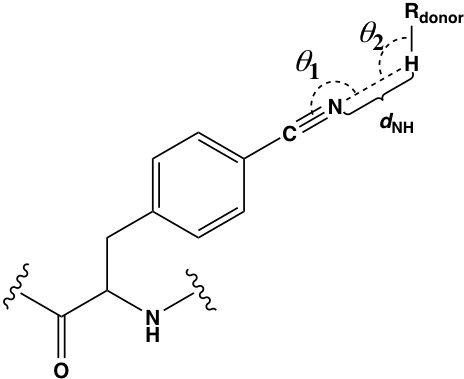
\includegraphics[width=3.25in]{figures-gfp-hbond/hbonding_scheme.png}
    \caption{Schematic of the hydrogen bonding geometric criteria. $\theta_1$ is the C--N$\cdots$H angle. $\theta_2$ is the N$\cdots$H--R$_{\text{donor}}$ angle, where R$_{\text{donor}}$ represents any hydrogen bond donor. $d_{\text{NH}}$ is the distance between the hydrogen and the acceptor nitrogen. In this analysis, any O, N, S, C$_{\alpha}$ atom was considered to be a potential hydrogen bond donor. To be considered a hydrogen bond, $\theta_1$ must be greater than \ang{99}, $\theta_2$ must be greater than \ang{120}, and $d_{\text{NH}}$ must be less than 2.45 \si{\angstrom}.}
    \label{fig:hbond-scheme}
\end{figure}

\subsection{Hydrogen bonds donated from water}

Hydrogen bonding interactions between the nitrile and water were analyzed for each snapshot of the nine MD simulations of CNF containing variants.
For each hydrogen bond, the geometry was calculated, and the different geometries were binned by $\theta_1$ and $d_{\text{NH}}$.
These results are plotted as heat maps in Figure \ref{fig:hbond-heatmap}A.
Hydrogen bonding geometries were also binned according to $\theta_2$ and $d_{\text{NH}}$.
However, the $\theta_2$ and $d_{\text{NH}}$ distributions (Figure \ref{fig:hbond-heatmap}) did not vary greatly across the nine systems (data not shown), and therefore contained less information.
For the rest of these analyses, we will focus primarily on $\theta_1$ as the determinant angle.
Figure \ref{fig:hbond-heatmap}A shows that several different hydrogen bonding geometries between the nitrile probes and water were present in our MD simulations.
The nitriles at positions 114, 117, 198, and 212 experienced broad distributions of hydrogen bonding angles, with each distribution covering the entire range of allowed angles (\ang{99} to \ang{180}).
This type of hydrogen bonding profile is consistent with a large degree of solvent exposure, where the hydrogen bonds are free to take on many orientations.
A representative snapshot of CNF in a solvent exposed position is shown in Figure \ref{fig:hbond-snapshot}A.
In contrast, Figure \ref{fig:hbond-heatmap}A shows the nitriles at position 145 and 218 experienced a much narrower distribution of hydrogen bonds, with hydrogen bonding angles localized between \ang{110} and \ang{150}.
A representative snapshot of a hydrogen bond between water and CNF 145 is shown in Figure \ref{fig:hbond-snapshot}B, and a representative snapshot of a hydrogen bond between water and CNF 218 is shown in Figure \ref{fig:hbond-snapshot}C.
These specific hydrogen bond geometries will be discussed in more detail below.
The nitriles at positions 92 and 143 experienced very few hydrogen bonds from water throughout the simulation (Figure \ref{fig:hbond-heatmap}A).
The nitrile at position 165 experienced slightly more hydrogen bonding from water than position 92 and 143, with two distinct geometries, one centered near \ang{150} and one centered near \ang{100} (Figure \ref{fig:hbond-heatmap}A).
Even using only three geometric parameters and considering only hydrogen bonds from water, we observed that CNF at these nine locations experienced a wide variety of possible hydrogen bonding interactions.
Clearly, a Boolean classification of hydrogen bonding is insufficient to describe the individual positions of each nitrile vibrational probe used in this work. 

\begin{figure}
    \center
    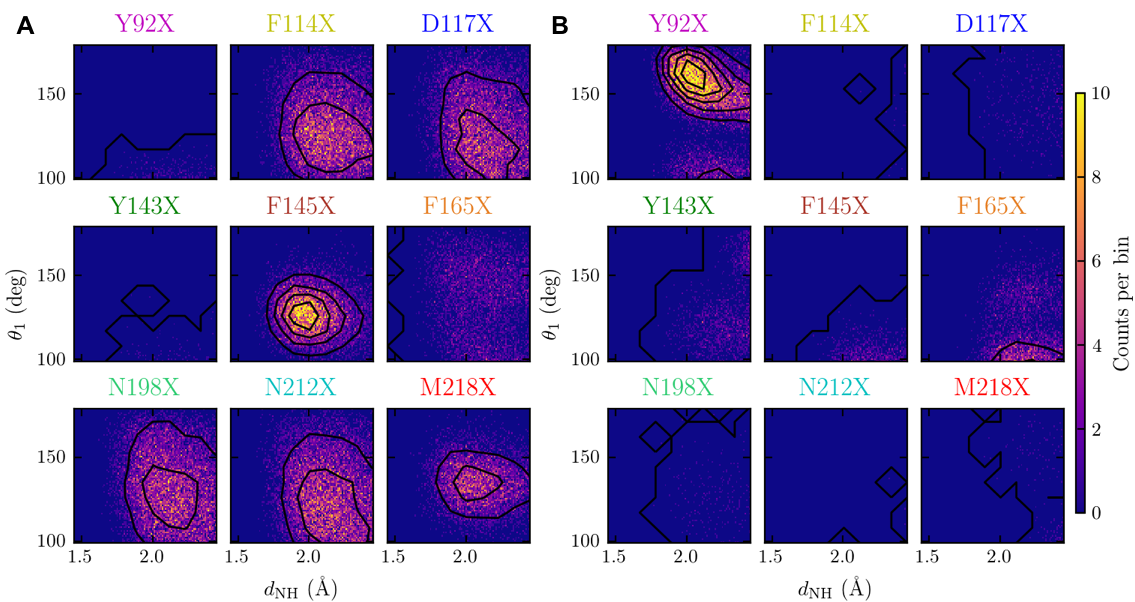
\includegraphics[width=6.5in]{figures-gfp-hbond/Figure6_combined.png}
    \caption{Heat maps of the hydrogen bonding geometries to CNF at each probe location. The titles are colored to correspond to the color codes used elsewhere in the paper. The hydrogen bonding geometries to CNF were calculated at each snapshot (every 4 ps) of the last 40 ns of a 50 ns MD simulation. Contour lines are drawn to guide the eye. $d_{\text{NH}}$ ($x$-axis) and $\theta_1$ ($y$-axis) are defined in Figure \ref{fig:hbond-scheme}. (A) Hydrogen bonds that are donated specifically from water, where R$_{\text{donor}}$ is the oxygen atom of a water molecule. (B) Hydrogen bonds that are donated from protein, where R$_{\text{donor}}$ may be any N, O, S, or C$_{\alpha}$ atom on the protein.}
    \label{fig:hbond-heatmap}
\end{figure}

\begin{figure}
    \center
    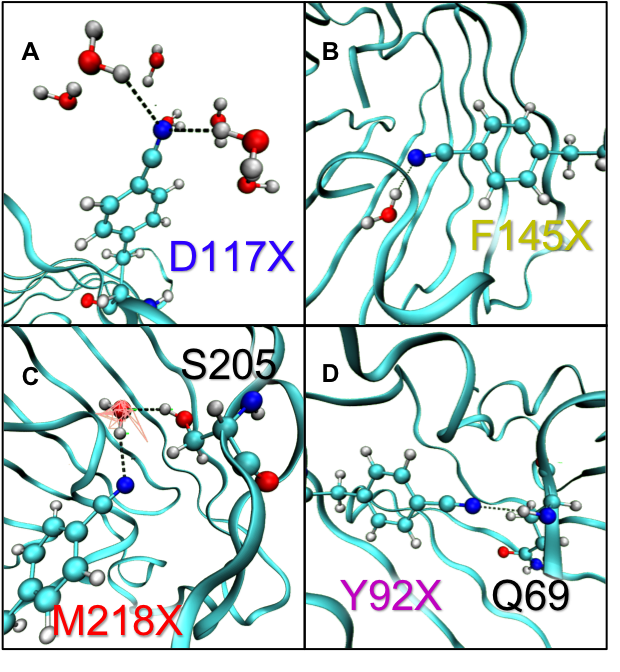
\includegraphics[width=3.25in]{figures-gfp-hbond/snapshots.png}
    \caption{Representative snapshots of select hydrogen bonding configurations observed in simulation. (A) The nitrile at position 117 was solvent exposed and involved in multiple simultaneous hydrogen bonds that exchanged frequently throughout the simulation. (B) The nitrile at position 145 was involved with a $\pi$-hydrogen bond with a confined water molecule, where $\theta_1$ was approximately \ang{120}. (C) The nitrile at position 218 was involved in a hydrogen bond with a confined water molecule, which is also hydrogen bound to the OH group of Ser205. The Connolly surface computed with gmx sasa is shown in pink lines to emphasize how a small available SASA can still have significant hydrogen bonding. (D) The nitrile at position 92 was involved in a linear hydrogen bond with the amide hydrogen of Gln69, where $\theta_1$ was approximately \ang{180}.}
    \label{fig:hbond-snapshot}
\end{figure}

\subsection{Hydrogen bonds donated from protein}

In addition to hydrogen bonds from water, we also investigated possible hydrogen bonds formed between the nitrile and donors from protein moieties.
Specifically, any O, N, S, or C$_{\alpha}$ atom in the protein was considered to be a possible hydrogen bond donor.
For each hydrogen bond between the nitrile and a protein donor, the geometry of the interaction was calculated and binned, and the results are shown as a heat map in Figure \ref{fig:hbond-heatmap}B.
Most nitrile locations (114, 117, 145, 198, 212, and 218) did not experience significant hydrogen bonding to donors from the protein.
However, the nitriles at positions 143 and 165 experienced some hydrogen bonding from the protein, and the nitrile at position 92 experienced extensive hydrogen bonding from a protein donor.
To investigate these protein-donated hydrogen bonding populations, we inspected the trajectories of each nitrile location.
For the nitrile at location 165, we found that the nitrile accepted transient hydrogen bonds from nitrogen atoms on two different nearby side chains (Arg96 and Gln183), leading to the two distinct populations shown in Figure \ref{fig:hbond-heatmap}B.
For the nitrile at position 143, we found that the nitrile accepted hydrogen bonds from a nitrogen on nearby Lys207, and interestingly the nitrile also accepted transient hydrogen bonds from the C$_{\alpha}$ of nearby Met218.
Carbon donated hydrogen bonds, especially from C$_{\alpha}$ atoms to nearby oxygen atoms, are common in proteins and have been under investigation for some time \cite{Wahl1997, Scheiner2011, Horowitz2012}, but this is the first evidence to our knowledge of a carbon-nitrile hydrogen bond.
Finally, at position 92, we found that the nitrile had a high probability of accepting a linear hydrogen bond from the amide hydrogen of Gln69.
A representative snapshot of this interaction is shown in Figure \ref{fig:hbond-snapshot}D and will be discussed in more detail below.
The observation that several of these CNF probes in the interior of GFP were engaged in hydrogen bonds with protein donors leads us to believe that because hydrogen bonds to the nitrile are so energetically favorable, the nitrile will accept weak hydrogen bonds from unconventional donors rather than remain isolated.  

%%%%%%%%%%%%%%%%%%%%%%%%%%%%%%%%%%%%%%%%%%%%%%%%%%%%%%%%%%%%%%%%
%%%%%%%%%%%%%%%%%%%%%%%%%%%%%%%%%%%%%%%%%%%%%%%%%%%%%%%%%%%%%%%%
\section{Discussion}\index{discussion}
%%%%%%%%%%%%%%%%%%%%%%%%%%%%%%%%%%%%%%%%%%%%%%%%%%%%%%%%%%%%%%%%
%%%%%%%%%%%%%%%%%%%%%%%%%%%%%%%%%%%%%%%%%%%%%%%%%%%%%%%%%%%%%%%%

\subsection{Relationship between FTLS and SASA}

To assess if the FTLS is a good measure of hydrogen bonding interactions, we plotted the measured FTLS against the ensemble averaged SASA of the CNF residues from simulation in Figure \ref{fig:hbond-comparison}A.
Our results show that there is a strong correlation between FTLS and SASA ($r = -0.920$), with two outliers (positions 92 and 218) that are not included in the regression fit.
We also performed this analysis using the SASA calculations of the aromatic sidechain atoms and the nitrile alone (from Figure S2).
The resulting comparisons can be found in Figure S3 in the Supporting Information.
While the trends in Figures S8A and S3 are consistent, because the relative standard deviations of the SASA increase dramatically as the region of the calculation is reduced, we have chosen to focus on the SASA values calculated for all atoms of the CNF residue.
The correlation between FTLS and SASA indicates that the CNF probes in locations that have higher SASA, and therefore higher potential hydrogen bonding interactions with water, show a greater change in the nitrile absorption frequency as temperature is changed.
The two outliers of positions 92 and 218 experienced hydrogen bonds that are not well described by SASA calculations and will be discussed in more detail below.
The SASA calculations for position 117 and 198 have larger standard deviations than the rest of the data.
Examining snapshots from the MD simulations revealed that CNF 117 alternated between two states with different SASAs through a torsional rotation about $\chi_1$ of CNF.
Similarly, CNF 198 drifted from a state of high SASA to a state of lower SASA over the course of the simulation.
These two examples of complex dynamic behavior of the CNF side chain indicate that enhanced MD sampling of CNF and/or its environment could lead to an even more quantitative relationship between SASA and FTLS; we are currently investigating this hypothesis. 

It is important to note that not all hydrogen bonding environments are captured by a calculation of the SASA.
For the two outliers discussed previously, CNF 92 and 218, we saw that the nitriles in these two locations experienced hydrogen bonding interactions that were not well described by SASA.
The data in Figure \ref{fig:hbond-heatmap} clearly demonstrate that CNF 92 was involved in a strong linear hydrogen bond with the amide hydrogen of Gln69, a representative snapshot of which is shown in Figure \ref{fig:hbond-snapshot}D.
Since this interaction was not due to solvent, it was not captured by the SASA.
In this case, relying only on the SASA calculation would have resulted in the incorrect conclusion that this nitrile was in an environment free from hydrogen bonding.
The FTLS, however, was the largest of any of the probe locations.
This leads us to believe that nitriles in buried locations as predicted by the calculation of SASA can still be involved in significant hydrogen bonding, and that SASA should not solely be relied upon for evaluating the hydrogen bonding potential of a probe location.
Further, we believe that this shows that in such cases the FTLS still provides a good experimental measure of hydrogen bonding interactions of the nitrile.
Because the FTLS was large over the temperature range measured in this particular case, we hypothesize that at increased temperatures, the thermal fluctuations of the protein backbone will increase and break the linear hydrogen bond between CNF 92 and the protein backbone, resulting in a large FTLS. 

\begin{figure}
    \center
    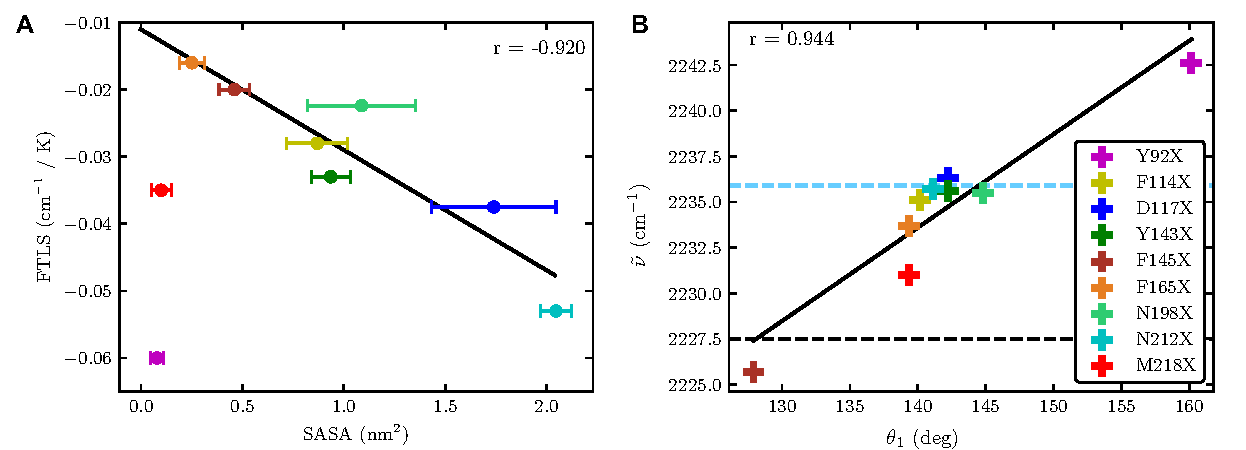
\includegraphics[width=6.5in]{figures-gfp-hbond/Figure8_combined.pdf}
    \caption{(A) The ensemble averaged SASA of the CNF residue plotted against the measured FTLS. The error bars on the $x$-axis are the standard deviations of the calculated SASAs. The regression line (black) does not include the nitrile at position 92 (purple) or 218 (red). These outliers are discussed in the main text. (B) For each of the nine nitrile locations, the average angle of hydrogen bonding from simulation is plotted against the experimental mean vibrational frequency. For reference, the mean vibrational frequency of CNF in water is shown as a light-blue dashed line, and the mean vibrational frequency of \emph{p}-tolunitrile in THF is shown as a black dashed line. All vibrational frequencies shown here were measured at 25\si{\celsius}.}
    \label{fig:hbond-comparison}
\end{figure}

Additionally, CNF 218 had a very low SASA, but the data in Figure \ref{fig:hbond-heatmap}A clearly show extensive hydrogen bonding to the solvent.
While the entire residue was surrounded by protein, leading to low SASA values, the nitrile group itself pointed directly to a single confined water stabilized by a hydrogen bond to Ser205, a representative snapshot of which is shown in Figure \ref{fig:hbond-snapshot}C.
This water formed hydrogen bonds with CNF 218 and could not easily diffuse away from the nitrile when the hydrogen bond was broken.
While the water molecule exchanged throughout the simulation, it did so rarely.
Because the small SASA was occupied with a hydrogen bonding water molecule, the calculated SASA underestimated the hydrogen bonding interactions.
In this case again, relying solely upon the calculated SASA would have led to the incorrect conclusion that this nitrile location was free from hydrogen bonding, while the measured FTLS still captured the hydrogen bonding interactions.
We interpret the FTLS of CNF 218 to indicate that this water is more likely to exchange with increased temperature, weakening the hydrogen bonding interaction to the nitrile and shifting the frequency.
We are currently investigating both of these hypothesized interpretations of the FTLS with additional simulations at varying temperatures.

These two observations from the MD trajectories of CNF 92 and 218 provide clear and direct explanations as to why they are outliers of the otherwise strong correlation between SASA and FTLS shown in Figure \ref{fig:hbond-comparison}A.
When the collection of nitrile locations is taken together, it is apparent that the temperature dependence of the nitrile frequencies is directly related to their respective hydrogen bonding environments in a quantitative manner.
These measurements demonstrate that the FTLS may be used to assess whether or not a particular nitrile location experiences a change in specific hydrogen bonding interactions as a result of some perturbation, such as an amino acid mutation or ligand docking event.
This would therefore allow the change in nitrile frequency to be attributed to that particular perturbation, and not to a change in specific hydrogen bonding environment.

\subsection{Nitrile frequency interpretations}

With the MD simulations of CNF containing GFP mutants and the predicted effects of hydrogen bond angle on the nitrile frequency reported by Choi et al. \cite{Choi2008}, we now have a straightforward way to interpret the relative frequency of our nitrile absorption spectra that would not have otherwise been possible.
The solvent exposed probes at positions 114, 117, 198, and 212 all had very similar FTIR absorption spectra, with frequencies centered on $\sim$2238 \si{\wn} and peak widths of $\sim$10 \si{\wn}.
Accordingly, the MD simulations showed that all four had similar water hydrogen bonding geometry profiles (Figure \ref{fig:hbond-heatmap}A) and the four largest SASA values (Figure \ref{fig:hbond-sasa}).

To see whether the nitrile frequency predictions reported by Choi et al. could be used in other cases, we extended this analysis to the CNF probe locations that experienced different hydrogen bonding geometries.
For example, the mean vibrational frequency of the nitrile at position 145 was the most red-shifted of any of the spectra and had the narrowest fwhm.
In simulation, CNF 145 was involved frequently in a hydrogen bond to water at $\sim$\ang{120} (Figure \ref{fig:hbond-snapshot}B).
In agreement with our experimental observations, Choi et al. predicted that these $\pi$-hydrogen bonds to nitriles red-shift the stretching frequency.
Additionally, hydrogen bonds to CNF 145 were more constrained with a smaller angle distribution than any other probe, corresponding to the narrow fwhm of the measured FTIR spectrum. 

Similarly, we found that the nitrile at position 218 was also involved in $\pi$-hydrogen bonding (Figure \ref{fig:hbond-snapshot}C) but with a larger maximum angle probability than that of CNF 145 by $\sim$\ang{10}.
Consistent with the predictions from the Cho group for $\pi$-hydrogen bonding, the frequency of the nitrile at position 218 was blue-shifted relative to the nitrile at position 145, but also red-shifted relative to all the other probe locations (Figure \ref{fig:hbond-spectra}).
This spectrum was again quite narrow, consistent with the MD simulation information of a constricted hydrogen bond. 

The two nitrile locations (143 and 165) that experienced the fewest hydrogen bonds of any of the locations are more difficult to interpret in this manner.
Nevertheless, the few hydrogen bonds experienced by the nitrile at position 143 are of similar $\theta_1$ (centered around \ang{145}) to the solvent exposed residues.
Experimentally, its mean vibrational frequency was also similar to the solvent exposed residues.
The nitrile at position 165 experienced a small population of hydrogen bonds from protein at sharp angles ($\sim$\ang{100}, Figure \ref{fig:hbond-heatmap}B), and while this angle should red-shift the frequency, the effect is small due to the size of the population.
Correspondingly, the absorbance frequency of the nitrile at position 165 is red-shifted relative to the solvent exposed residues, but not as red-shifted as positions 92 and 218. 

Finally, we found a direct interpretation of the far blue-shifted spectrum of the nitrile at position 92.
In the absence of any molecular level information, the interpretation of this spectrum would be very difficult, because this location is in the interior of the $\beta$-barrel, removed from potential bulk water hydrogen bonds.
However, the simulations revealed that the nitrile at this location was involved in a strong linear hydrogen bond (Figure \ref{fig:hbond-snapshot}D) to the amide backbone of Gln69.
Such $\sigma$-hydrogen bonds are predicted by the Choi et al. to blue-shift the spectra by withdrawing electron density from the antibonding molecular orbital of the nitrile, increasing the overall bond order of the group and shortening the bond, leading to higher frequency \cite{Getahun2003, Adhikary2014, Eaton1988}.
Additionally, we found that there were two distinct hydrogen bonding populations for the nitrile at this location.
While the dominant population was linear ($\sim$160-\ang{180}) and blue-shifting, there was a smaller population at a smaller $\theta_1$ ($\sim$\ang{100}).
This smaller population caused a lowering of the nitrile frequency relative to the linear hydrogen bonded population and resulted in a broadening of the experimental FTIR spectrum.
Indeed, the nitrile at position 92 had the largest fwhm, and was the only mutant from the MD trajectories that had two significant hydrogen bonding populations that occurred at sharply different angles. 
To quantify the effect of hydrogen bonding geometry on the measured nitrile frequencies, we binned all of the hydrogen bonding geometries observed for each probe by angle and fit a polynomial to smooth the noise of the histogram (Figure S4A).
Because of the geometric considerations of the hydrogen bonding probability \cite{Kroon1975}, we calculated the probability density for each angle for $\theta_1$ by normalizing by the volume element of each angular bin, calculated via Equation \ref{eq:angnorm}: 
\begin{equation}
    V = \frac{2\pi d^3_{\text{NH}}}{3}(\cos(\pi-\theta_1') - \cos(\pi - \theta_1'')) 
    \label{eq:angnorm}
\end{equation}
Here, $V$ is the volume element of the bin, $\theta_1'$ and $\theta_2''$ are the bin edges of $\theta_1$, and $d_{\text{NH}}$ is the maximum hydrogen bond distance.
The normalized probability densities are shown in Figure S4B.
ne then took the weighted average of all the hydrogen bonds by probability (black vertical line in Figure S4B) and plotted this average angle against the mean vibrational frequency of each nitrile in Figure \ref{fig:hbond-comparison}B. 

For all nine probe locations investigated, we observed a strong correlation ($r = 0.944$) between the hydrogen bonding angle and the mean vibrational frequency, as Choi et al. predicted in their quantum mechanical calculations \cite{Choi2008}.
The strength of the correlation is somewhat surprising given the well-known inaccuracies of hydrogen bonding geometries in the Amber03 force field \cite{Paton2009}, and that we have not accounted for electrochromic effects contributing to the measured frequencies or for exchange-repulsion interaction-induced frequency shifts.
These two effects are expected to also influence the measured vibrational frequency.  

To account electrochromic effects that may contribute to the measured frequency, we estimated the extent of the Coulombic frequency shift by calculating the Coulombic field at the midpoint of the nitrile using a procedure described elsewhere \cite{Ensign2011}.
The calculated electric field is plotted against the mean vibrational frequency in the Supporting Information (Figure S5).
The calculated electric fields are poorly correlated to the mean vibrational frequency, suggesting that electrochromic effects play a minor role in contributing to the measured frequency.
We separately investigated the extent of the exchange-repulsion interaction-induced frequency shift in these systems by analyzing the hydrogen bond length parameter, $d_{\text{NH}}$.
The histograms and normalized probability densities for each hydrogen bonding distance bin are in the Supporting Information (Figure S6), and the average distance is plotted against the mean vibrational frequency in Figure S7.
However, presumably because each of these distance interactions are governed by the same Lennard Jones potential from the Amber03 force field, the probability distributions of the lengths of hydrogen bonds to water are remarkably similar.
Thus, the average hydrogen bond distances are not well correlated to the experimental mean vibrational frequencies.
Because of the strong correlation of the hydrogen bonding angle, the lack of correlation of the calculated Coulombic field, and the lack of correlation of the average hydrogen bonding distance, we believe that the hydrogen bonding angle is the dominant contribution to the frequency in these cases.

In order to contribute to the line shape of the nitrile spectra, a given hydrogen bond would need to have a lifetime longer than the vibrational lifetime of the nitrile probe.
To determine whether or not that was the case for the hydrogen bond populations in Figure \ref{fig:hbond-heatmap}, we tracked each hydrogen bond in all nine trajectories.
As a function of simulation time, we plotted the number of hydrogen bonds that persisted for at least that length of time.
These plots were fit to an exponential decay function and are shown in the Supporting Information (Figure S8).
The lifetimes were calculated from the decay rate and are reported in Table S2.
All but one hydrogen bonding population had a lifetime approximately equal to or longer than the vibrational lifetime of CNF, which is estimated to be on the order of a picosecond or less \cite{Ghosh2009, Ha2009, Waegele2010}, suggesting that these populations contribute to the line shape of the nitrile absorption spectrum.

It is interesting to note that out of all of our nine protein systems, not a single nitrile location was free from hydrogen bonding.
While this certainly may be an artifact of GFP with its unique water filled $\beta$-barrel structure, it appears that hydrogen bonding to the nitrile is so favorable that even when placed in a location with no solvent accessibility, the nitrile will find a donor other than water.
For example, when we put the nitrile at position 92, a location with virtually no solvent exposure, we observed that the nitrile was involved in significant hydrogen bonding with protein atoms.
Additionally, when we put the nitrile at position 143, a location that was void of any conventional hydrogen bond donors, the nitrile experienced transient hydrogen bonds from an electron poor carbon atom.
The observation of these weak hydrogen bonds from carbon suggests that even if there are no strong hydrogen bond donors nearby, the nitrile will still engage in interactions to fulfill its hydrogen bond accepting capabilities.
If these observations of nitrile-labeled GFP extend to other systems, this would certainly complicate the interpretation of nitrile spectra in biological systems.
Our results suggest that, to properly interpret nitrile spectra, one must \emph{always} consider hydrogen bonding effects.
Because of the consistent presence of hydrogen bonds and the strong correlation between the hydrogen bonding angle and the mean vibrational frequency, it is necessary to determine the geometry of hydrogen bonds to the nitrile in all reference and perturbed states to ensure that the measured frequency shifts are not due to change in hydrogen bond geometry.
A constant frequency offset, such as the 10 \si{\wn} offset suggested by Fafarman et al. \cite{Fafarman2010}, cannot be applied to nitrile frequencies in protein systems where the hydrogen bonding orientation is easily constrained by the protein surroundings, such as an enzyme active site or in the interior of a protein.
Specifically, when measuring a particular perturbation via vibrational spectroscopy of a nitrile, the FTLS of the reference and perturbed state may be used to confirm that specific hydrogen bonding interactions do not change substantially between the two states.

Certainly, we have shown that a Boolean classification of the existence of hydrogen bonding is insufficient when the nitrile is placed in complex protein environments.
There is a broad range of hydrogen bonding interactions available to a nitrile probe, and each circumstance contributes differently to the nitrile frequency.
This means that there is not a constant change in frequency that can universally be applied to all hydrogen bonding interactions.
However, the ability of nitriles to accept hydrogen bonds should not be interpreted as a disadvantage for its use as a vibrational probe.
The strength of the correlation in Figure \ref{fig:hbond-comparison}B demonstrates that is possible to decouple the hydrogen bonding shift from other spectroscopic effects, such as the VSE, when there is sufficient molecular information about the hydrogen bonding geometry and FTLS.

%%%%%%%%%%%%%%%%%%%%%%%%%%%%%%%%%%%%%%%%%%%%%%%%%%%%%%%%%%%%%%%%
%%%%%%%%%%%%%%%%%%%%%%%%%%%%%%%%%%%%%%%%%%%%%%%%%%%%%%%%%%%%%%%%
\section{Conclusions}\index{hbond-conclusion}
%%%%%%%%%%%%%%%%%%%%%%%%%%%%%%%%%%%%%%%%%%%%%%%%%%%%%%%%%%%%%%%%
%%%%%%%%%%%%%%%%%%%%%%%%%%%%%%%%%%%%%%%%%%%%%%%%%%%%%%%%%%%%%%%%

We have experimentally measured the temperature-dependent frequencies of CNF in nine different locations across the GFP protein and demonstrated the broad range of hydrogen bonding environments present in a complex protein system.
We showed that the FTLS is directly related to molecular level details of the specific hydrogen bonding interactions to the nitrile probe.
The FTLS is strongly correlated to the SASA of the CNF probe, except in cases where constrained molecular geometry resulted in significant hydrogen bonding that was not captured by SASA.
Nevertheless, it appears the FTLS of a nitrile probe can be used to rapidly assess the degree of hydrogen bonding of the nitrile, even in the dynamic and complex environment found in and around a protein.
These molecular-level details are essential for properly interpreting the vibrational spectrum of the nitrile probe in any experiment where the specific hydrogen bonding interactions may be changing.
This is especially necessary to ensure that a VSE experiment is actually reporting on a change in electric field instead of reflecting sensitivity to subtle changes in hydrogen bonding geometries. 

We have further demonstrated the significant effect of hydrogen bonding on the nitrile spectra by showing that in our nine CNF containing variants, the mean nitrile vibrational frequency was dominated by the hydrogen bonding geometry, and that the measured frequencies matched what was expected from a theoretical prediction of the effect of hydrogen bonding geometry on nitrile frequency.
In every one of our systems, the CNF probe experienced some type of hydrogen bonding.
For all observed variants, the average hydrogen bonding angle was well correlated with the mean vibrational frequency observed in experiment.
Additionally, the fwhm of the experimental spectra were qualitatively consistent with the distribution of the hydrogen bonding geometries from simulation.
Finally, we have shown that FTLS measurements may be used to assess the hydrogen bonding interactions of a nitrile so that they may be properly accounted for in the interpretation of the spectra.







\chapter{INSERT FINAL SNASE TITLE HERE}\label{snase}

This is a place holding for the SNase draft. 


\chapter{Quantitative Measurement of Intrinsic GTP Hydrolysis for
Carcinogenic Glutamine 61 Mutants in H-Ras} \label{ras}

\newcommand{\RalBSCN}{{Ral$\beta$I18C$_{\text{SCN}}$}}
\newcommand{\RalB}{{Ral$\beta$}}


Mutations of human oncoprotein p$^{21}$H-Ras (hereafter ``Ras'') at glutamine 61 are known to slow the rate of guanosine triphosphate (GTP) hydrolysis and transform healthy cells into malignant cells. 
It has been hypothesized that this glutamine plays a role in the intrinsic mechanism of GTP hydrolysis by interacting with an active site water molecule that stabilizes the formation of the charged transition state at the $\gamma$-phosphate during hydrolysis.
However, there is no comprehensive data set of the effects of mutations to Q61 on the protein's intrinsic catalytic rate, structure, or interactions with water at the active site. 
Here, we present the first comprehensive and quantitative set of initial rates of intrinsic hydrolysis for all stable variants of RasQ61X. 
We further conducted enhanced molecular dynamics (MD) simulations of each construct to determine the solvent accessible surface area (SASA) of the side chain at position 61 and compared these results to previously measured changes in electric fields caused by RasQ61X mutations. 
For polar and negatively charged residues, we found that the rates are normally distributed about an optimal electrostatic contribution, close to that of the native Q61 residue, and the rates are strongly correlated to the number of waters in the active site. 
Together, these results support a mechanism of GTP hydrolysis in which Q61 stabilizes a transient hydronium ion, which then stabilizes the transition state while the $\gamma$-phosphate is undergoing nucleophilic attack by a second, catalytically active water molecule. 
We discuss the implications of such a mechanism on future strategies for combating Ras-based cancers.

%%%%%%%%%%%%%%%%%%%%%%%%%%%%%%%%%%%%%%%%%%%%%%%%%%%%%%%%%%%%%%%%
%%%%%%%%%%%%%%%%%%%%%%%%%%%%%%%%%%%%%%%%%%%%%%%%%%%%%%%%%%%%%%%%
\section{Publication note} \label{ras-pub-note}
%%%%%%%%%%%%%%%%%%%%%%%%%%%%%%%%%%%%%%%%%%%%%%%%%%%%%%%%%%%%%%%%
%%%%%%%%%%%%%%%%%%%%%%%%%%%%%%%%%%%%%%%%%%%%%%%%%%%%%%%%%%%%%%%%

Portions of this chapter are adapted from the following publication: 

\noindent Elisa T. Novelli, Jeremy T. First, Lauren J. Webb; Quantitative Measurement of Intrinsic GTP Hydrolysis for Carcinogenic Glutamine 61 Mutants in H-Ras. \emph{Biochemistry}. \textbf{2018}, \emph{57}, 6356-6366.

%%%%%%%%%%%%%%%%%%%%%%%%%%%%%%%%%%%%%%%%%%%%%%%%%%%%%%%%%%%%%%%%
%%%%%%%%%%%%%%%%%%%%%%%%%%%%%%%%%%%%%%%%%%%%%%%%%%%%%%%%%%%%%%%%
\section{Introduction} \label{ras-intro}
%%%%%%%%%%%%%%%%%%%%%%%%%%%%%%%%%%%%%%%%%%%%%%%%%%%%%%%%%%%%%%%%
%%%%%%%%%%%%%%%%%%%%%%%%%%%%%%%%%%%%%%%%%%%%%%%%%%%%%%%%%%%%%%%%

The Ras superfamily of approximately 150 GTPases consists of signaling proteins that hydrolyze guanosine triphosphate (GTP) to guanosine diphosphate (GDP) to switch between ON (GTP-bound) and OFF (GDP-bound) states in a variety of signal transduction pathways \cite{Bourne1991, Krauss2003}.
There are multiple inputs and outputs in this catalytic cycle: (1) Ras-like GTPases interact with multiple downstream effector proteins to facilitate signaling in the ON state and propagate a signaling cascade; (2) GTPase activating proteins (GAPs) bind to Ras and facilitate GTP hydrolysis, converting Ras to the OFF state; and (3) exchange factor proteins (GEFs) bind to Ras to promote the exchange of GDP for GTP to return Ras to the ON state \cite{Krauss2003, Cherfils2013, Khrenova2015}.
A canonical member of this superfamily, p$^{21}$H-Ras (hereafter ``Ras''), is part of a signaling pathway that regulates cell survival and proliferation \cite{Shields2000, Cox2003, Downward2003, Repasky2004, Prior2012}.
Mutations to Ras that slow hydrolysis and leave the protein in an ON state can lead to uncontrolled cell growth and tumorigenesis \cite{Prior2012}. 
A recent survey found that mutations to the Ras family of genes appear in approximately 16\% of cancer tumors, with some specific types such as pancreatic tumors showing far greater mutation frequencies \cite{Prior2012}. 
Because of its role as a molecular switch, the oncogenic properties of Ras are intimately tied to the kinetics of the GTP hydrolysis reaction.

Since the discovery of Ras in 1964\cite{Harvey1964}, three key residues have been identified that, when mutated, are present in the vast majority of Ras-induced tumor cells: G12, G13, and Q61 \cite{Prior2012}.
The effects of mutations to the native glycine residues at positions 12 and 13 have been well studied and are largely considered to result from steric effects on the folding and dynamics of the enzyme near the active site \cite{Prior2012, Bos1989, Eccleston1993, Hobbs2016}.
However, the role of Q61 in the hydrolysis mechanism is more puzzling and has been debated continuously in the literature \cite{Kamerlin2013, Carvalho2015}.
In a crystal structure solved in 1990, Pai et al. observed a water molecule that was positioned for in-line nucleophilic attack on the leaving phosphate group and postulated that Q61 acts as a general base to deprotonate the attacking water molecule and activate it for GTP hydrolysis \cite{Pai1990}. 
However, using theoretical calculations, Langen et al. demonstrated in 1992 that Q61 cannot act as the general base in such a mechanism because the activation energy for proton abstraction is too large to be consistent with the observed rate \cite{Langen1992}.
Further, in 2004, Shurki and Warshel\cite{Shurki2004} demonstrated that Q61 plays an indirect but significant role in the RasGAP-mediated mechanism of GTP hydrolysis by ``pre-organizing'' the active site of Ras to allow Arg789 of RasGAP (referred to as the ``arginine finger'') to insert into the active site and stabilize the transition state of the nucleophilic attack by water \cite{Scheffzek1997}. 
This RasGAP activity increases the hydrolysis reaction rate by a factor of $10^5$ \cite{Schweins1995}.
This mechanism of assisted hydrolysis has since been further studied and characterized \cite{Khrenova2015, Shurki2004, Grigorenko2005}.

However, the affinity of RasGAP for Ras is 3 orders of magnitude lower than that of Ras and its downstream effectors\cite{Vogel1988}, and so \emph{in vivo} Ras is primarily docked with a downstream effector. 
Because of this, therapeutic strategies for RasQ61X mutations must consider the protein when it is bound to its downstream effector, and thus GTP hydrolysis mostly occurs through an intrinsic, not assisted, mechanism. 
However, the molecular level details of this intrinsic mechanism of hydrolysis have remained elusive.

In 2010, Buhrman et al. proposed a new mechanism for intrinsic hydrolysis involving two water molecules, in which the catalytic water shuttles a proton to a bridging water molecule that is stabilized by hydrogen bonds to Q61 and Y32\cite{Buhrman2010}, as illustrated in Figure \ref{fig:ras-mech}A. 
This positively charged hydronium ion stabilizes the transition state in the intrinsic mechanism and partially fulfills the role of the ``arginine finger'' in the RasGAP-assisted hydrolysis mechanism, although with much lower efficacy. 
From this perspective, the role of Q61 is to stabilize the hydronium ion, which in turn stabilizes the transition state. 
This mechanism was suggested based on the appearance of a crystallographic water molecule in the pdb structure 3k8y\cite{Buhrman2010} but has not been confirmed through other experiments. 
However, it is further supported by the fact that, in separate work, the same group found that highly and moderately transforming (cancer causing) mutants of Q61 tended to be buried and occluded from solvent, while weakly and nontransforming (noncancer causing) mutations were solvent exposed \cite{Buhrman2007}. 
This supports the idea that water is crucial to the intrinsic hydrolysis mechanism. If this hypothesis is correct, then Q61 can be thought of as participating electrostatically, not chemically, in GTP hydrolysis, and so a careful interrogation of the effects of the electric field in and around the active site at steady-state and during hydrolysis are important for proving this mechanism.

\begin{figure}
    \center
    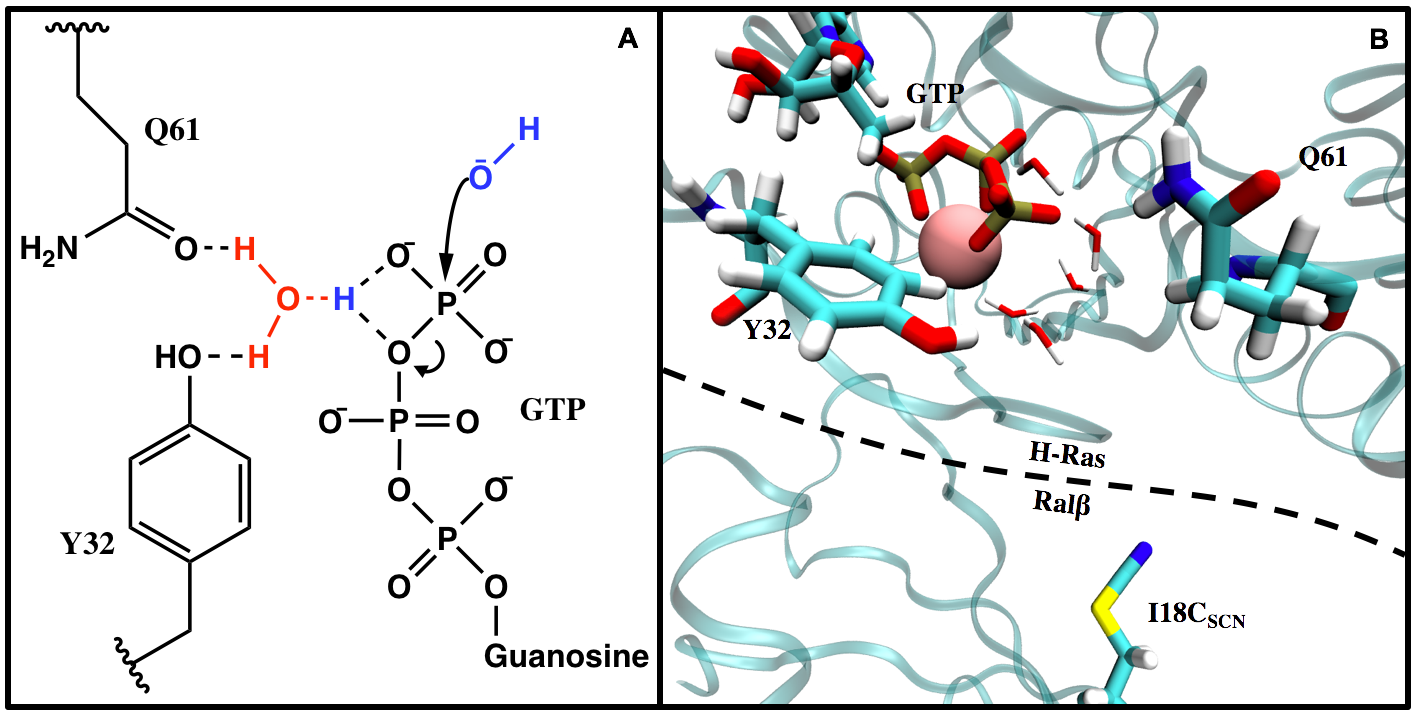
\includegraphics[width=\double]{figures-ras/Figure1_two_column.png}
    \caption{
        (A) A proposed multiwater mechanism of the intrinsic Ras GTPase reaction. 
        The catalytic water (blue) shuttles a proton to a nearby, stabilized water (red) via the $\gamma$-phosphate, adopted from ref \citenum{Buhrman2010} and ref \citenum{Stafford2012}. 
        (B) A snapshot of the Ras/\RalBSCN{} interface. 
        The ribbons in the background represent the backbone of the protein. 
        The sticks represent the relevant residues in the system: Y32 of Ras, Q61 of Ras, GTP, and \RalBSCN{}. 
        The pink sphere is \ce{Mg^2+}, and the small sticks represent water in the active site.
    }
    \label{fig:ras-mech}
\end{figure}

Previous work in our group has made use of vibrational Stark effect (VSE) spectroscopy to interrogate the electric field of the active site of Ras constructs with mutations at position 61 (RasQ61X, where X represents a mutation from the native Gln residue) \cite{Stafford2012}.
VSE spectroscopy takes advantage of the difference dipole moment, $\Delta\vec{\mu}$, inherent in small vibrational probes (in this case a nitrile), to relate shifts in the vibrational frequency, $\Delta E$, to changes in local electric field, $\Delta\vec{F}$, according to eq \ref{eq:ras-stark} \cite{Andrews2000, Andrews2002, Fafarman2006, Fried2015, Slocum2018}:

\begin{equation}
\Delta E = - \Delta\vec{\mu}\cdot\Delta\vec{F}
\label{eq:ras-stark}
\end{equation}

In that work, a nitrile probe was strategically incorporated at position 18 of the Ras binding domain of the downstream effector RalGDS (hereafter, \RalB{}), generating the construct \RalBSCN{} which denotes that the native isoleucine at position 18 was replaced with a cysteine, which was then post-translationally modified to cyanocysteine. 
Though a different protein, c-Raf kinase (Raf), is the primary downstream effector of Ras \emph{in vivo}, Raf has been shown to alter some rates of intrinsic hydrolysis \cite{Buhrman2011}.
By docking \RalBSCN{} with Ras, the nitrile group was well positioned to report on electric field changes due to mutations to Q61 in and around the Ras active site, without affecting the intrinsic hydrolysis mechanism. 
A snapshot of this system based on the pdb structure 1lfd is shown in Figure \ref{fig:ras-mech}B.

While nitrile spectra have also been shown to report on solvation environments due to quantum mechanical effects of specific hydrogen bonding \cite{Waegele2009, Oh2008,Fafarman2010}, here we show that the solvent exposure and specific hydrogen bonding interactions of the nitrile on \RalBSCN{} are identical between the Ras mutants. 
We therefore interpreted the shifts in vibrational frequency of the nitrile probe on \RalB{} as changes in local electric field, according to eq \ref{eq:ras-stark}, caused by mutations to Q61 in Ras across the protein-protein interface ($\sim$9 \si{\angstrom}). 
Because any multiwater intrinsic hydrolysis mechanism, such as that proposed by Buhrman et al., relies on noncovalent stabilization of water in the active site, we compared the shifts in nitrile frequency to quantitative measurements of the ability of the side chain to interact with water. 
We observed correlations between the nitrile shifts and both the solvent accessible surface area (SASA) and the hydration potential of the residue at position 61 \cite{Stafford2012}.
Based on these results, we hypothesized that the identity of the residue at position 61 affects the rate of intrinsic GTP hydrolysis through noncovalent and electrostatic stabilization of water molecules according to each residue's affinity for water, supporting a multiwater mechanism such as the one proposed in Figure \ref{fig:ras-mech}A.

In spite of the ongoing debate regarding the role of Q61 in the mechanism of intrinsic hydrolysis, there has not yet been a comprehensive quantitative examination of the role of Q61 mutations on the intrinsic hydrolysis rate. 
Though the literature has suggested that at least 17 Q61X intrinsic hydrolysis rates have been measured, most have not been explicitly reported and, to our knowledge, were measured only semiquantitatively \cite{Der1986}.
Fully quantitative intrinsic hydrolysis rate constants of RasQ61X mutations have only been reported for WT, E, H, and L \cite{Krengel1990, Frech1994}.

Here, we present measurements of the initial rate of intrinsic hydrolysis of GTP in WT and 17 RasQ61X constructs. 
Intrinsic rates were measured using a malachite green colorimetric assay based on the binding of malachite green indicator to a phosphomolybdate complex formed from the phosphate product of the hydrolysis reaction. 
This GTPase activity assay is useful because it is a sensitive and nonradioactive technique for detecting phosphate and has been successfully applied to other GTPase proteins \cite{Quan2005}.
To our knowledge, this is the first report of a comprehensive set of quantitative kinetics data for all Q61X mutations (except Q61P and Q61C, which could not be expressed). 
Our initial rate measurements indicated that, in most cases, mutations to position 61 resulted in significantly slower GTP hydrolysis. 
We compared our measured initial rates to previously published information on the electric field due to these mutations, measured by VSE spectroscopy \cite{Stafford2012}.
We found that the initial rate of intrinsic hydrolysis was related to the observed nitrile frequencies for residues that are able to stabilize the hypothesized hydronium ion (polar and negatively charged residues). 
No relationships were observed for amino acids with positively charged or nonpolar side chains.

Additionally, we used enhanced molecular dynamics (MD) simulations to determine the molecular basis for this relationship by calculating the SASA of the polar side chain atoms as well as the entire side chain of Q61X. 
We found that the reported vibrational frequencies were well correlated to the SASA of the side chain polar atoms in all polar and charged amino acids, while the initial rate of intrinsic hydrolysis was well correlated to the SASA of the entire side chain, but only for polar and negatively charged amino acids. 
For the polar and negatively charged residues, we found a strong correlation between the number of water molecules in the active site (determined from MD) and the initial rate of intrinsic hydrolysis.
This evidence strongly supports a multiwater mechanism, such as the mechanism proposed by Buhrman et al. and illustrated in Figure \ref{fig:ras-mech}A, where a positively charged hydronium ion stabilizes the transition state of the reaction. 
This kinetic data set is invaluable for understanding the intrinsic mechanism of hydrolysis and will provide insight for further computation and development of therapeutic strategies


%%%%%%%%%%%%%%%%%%%%%%%%%%%%%%%%%%%%%%%%%%%%%%%%%%%%%%%%%%%%%%%%
%%%%%%%%%%%%%%%%%%%%%%%%%%%%%%%%%%%%%%%%%%%%%%%%%%%%%%%%%%%%%%%%
\section{Materials and Methods} \label{ras-methods}
%%%%%%%%%%%%%%%%%%%%%%%%%%%%%%%%%%%%%%%%%%%%%%%%%%%%%%%%%%%%%%%%
%%%%%%%%%%%%%%%%%%%%%%%%%%%%%%%%%%%%%%%%%%%%%%%%%%%%%%%%%%%%%%%%

\subsection{Mutagenesis}

The gene for hexahistidine-tagged WT H-Ras, residues 1-166, was a gift of the Kuriyan laboratory \cite{Boriack-Sjodin1998}. 
A plasmid containing hexahistidine-tagged Tobacco Etch Virus Protease (His-TEV) with the S219V mutation in \emph{E. coli} Bl21(DE3)-RIL cells was a gift from David Waugh (Addgene plasmid 8827) \cite{Kapust2001}. 
The 97-residue Ras Binding Domain of \RalB{} was taken from residues 790-886 of RalGDS and numbered according to the pdb entry 1lfd \cite{Huang1998}. 
The gene was cloned and mutated as described previously \cite{Stafford2012, Stafford2010}.
Mutations to Q61 of Ras were made using the Quikchange Lightning site-directed mutagenesis kit (Agilent).

\subsection{Purification}

Plasmids encoding the WT and mutant Ras constructs were transformed into BL21(DE3) cells for expression. 
All proteins were expressed and purified as previously described \cite{Stafford2012, Kapust2001, Stafford2010}, with the exception of the buffers used for Ras, which were altered to minimize phosphate background in the kinetics experiments. 
All reagents were purchased from Sigma-Aldrich and used without further purification unless stated otherwise. 
Briefly, cells were collected and resuspended in loading buffer (50 mM Tris-HCl, 250 mM NaCl, 40 mM imidazole, 10\% glycerol, pH 7.5) for lysis via probe sonication followed by centrifugation to remove cell debris. 
The supernatant was loaded onto a nickel immobilized metal affinity column (Ni-IMAC, Fisher). 
His-tagged Ras proteins were eluted with an elution buffer (50 mM Tris-HCl, 250 mM NaCl, 500 mM imidazole, 10\% glycerol, pH 7.5). 
Protein was exchanged into a cleavage buffer (50 mM Tris, 50 mM KCl, 10\% glycerol, pH 8) with a PD-10 column (GE Healthcare) and cleaved with His-TEV at a ratio of approximately 1 mg His-TEV to 100 mg of His-Ras overnight at 4 \si{\celsius}. His-TEV and uncleaved Ras were removed by passing the solution through another Ni-IMAC column, and the cleaved protein was exchanged into final buffer (50 mM Tris, 100 mM NaCl, 10\% glycerol, pH 7.5) and either used immediately or flash frozen and stored at -80 \si{\celsius} for later use. 
To ensure that the active site of Ras contained GDP (OFF state) in preparation for kinetics experiments, the purified Ras was incubated with 5 mM dithiothreitol (DTT), 5 mM ethylenediamine tetraacetic acid (EDTA), and GDP in 100-fold excess of the protein concentration for 90 min on ice, and then 10 mM \ce{MgCl2} was added and the solution incubated for a further 30 min on ice. 
The GDP-containing protein was then buffer exchanged into kinetics buffer (50 mM Tris-HCl, 50 mM NaCl, 20 mM EDTA, 5 mM \ce{MgCl2}, 0.01\% Triton X-100, pH 7.5) for the kinetics experiments. 
The RasQ61C and RasQ61P mutations could not be expressed for reasons we have not investigated and are thus not presented here. 
The nitrile functional group on \RalB{} was introduced as previously described \cite{Stafford2010}.

\subsection{Kinetics}

The initial rates of hydrolysis of GTP by RasQ61X constructs were measured using the malachite green assay\cite{Quan2005, Hohenwallner1973, Lanzetta1979} to detect the production of inorganic phosphate. 
The hydrolysis product, \ce{Pi}, was detected through the formation of a colorless phosphomolybdate complex under acidic conditions, which reacted with malachite green indicator to form a colored product that was quantified by UV-vis absorption at 640 nm. 
The assay has a broad dynamic range (typically 1-200 $\mu$M) that was tailored to the reaction conditions based on the ratio of assay volume to malachite green detection reagent volume. 
The assay has the advantage of using GTP as the substrate instead of fluorescently labeled GTP, which introduces kinetic artifacts, or radiolabeled GTP, which has associated handling hazards and expenses.

The malachite green reagent contained ammonium molybdate and malachite green oxalate dissolved in 1 N HCl (all purchased from Sigma-Aldrich) and was made as described previously \cite{Quan2005}.
A 1 mM phosphate standard stock solution was made by drying the highest available purity \ce{K3PO4} in an oven at 110 \si{\celsius} overnight before dissolving in high purity water. 
Lower concentration standard solutions of \ce{K3PO4} for the calibration curve were serially diluted from the stock solution in kinetics buffer at the time of the experiment. 
The GTP substrate solution contained 40 $\mu$M GTP and 1 mM DTT in kinetics buffer. 
To minimize contamination that increased the phosphate background, we used the highest purity GTP available. 
Each reaction was initiated by mixing 20 $\mu$L of 8 mM RasQ61X with 20 $\mu$L of GTP substrate solution for a final assay reaction solution of 4 $\mu$M RasQ61X and 20 $\mu$M GTP. 
Reactions were incubated at 37 \si{\celsius} from 0 to 8 h by initiating the 8 h reaction first and then adding subsequent reactions to the incubator at each time point. 
All reactions were then transferred to a black, optical-bottom 384-well plate (Thermo Scientific) and all stopped at the same time through the addition of the malachite green reagent. 
Reactions were done at least in triplicate, and each reaction vial had enough volume for three wells, resulting in at least 9 measurements for each time point. 
Each well contained 10 $\mu$L of assay reaction and 30 $\mu$L of malachite reagent, and the optical response was linear (Figure \ref{fig:ras-response}) through the entire range of standards (0-25 $\mu$M phosphate). 
Absorption of the phosphomolybdate/malachite green colored complex was measured via a BioTek Synergy H4 plate reader at 640 nm using path length correction functionality to account for small differences in volume due to pipetting error.

\begin{figure}
    \center
    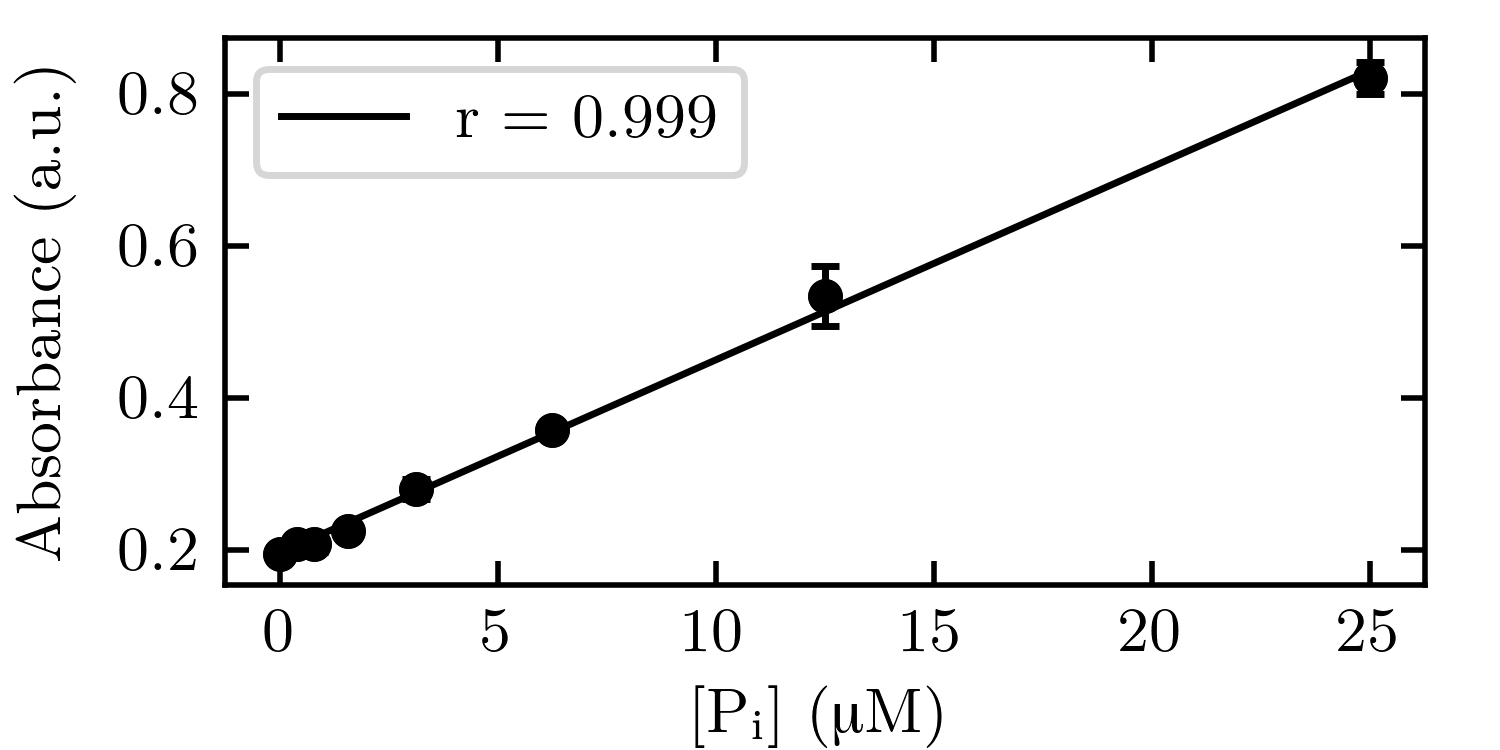
\includegraphics[width=\single]{figures-ras/optical_response.png}
    \caption{
        Calibration curve of the malachite green colorimetric assay collected from phosphate standards of 0.00, 0.39, 0.78, 1.56, 3.13, 6.25, 12.5, and 25 $\mu$M. 
        The response is linear over the range of phosphate concentration measured in our experiments.
    }
    \label{fig:ras-response}

\end{figure}

\subsection{MD and SASA Calculations} 

A template Ras/\RalB{}I18C docked complex with GTP and \ce{Mg^2+} in the binding site and all crystallized waters was modeled by homology from the 1lfd crystal structure\cite{Huang1998} using the MODELLER software package \cite{Marti-Renom2000, Sali1993, Fiser2000}, and the E31K mutation on Ras in the published structure was reverted to the wild-type glutamate. 
From this structure, I18C of \RalB{} was further modified to cyanocysteine and independently minimized using the Avogadro molecular editing package \cite{Hanwell2012}. 
Using this template, 15 separate mutations from the WT Q61 residue of Ras to all residues except A, G, C, and P were made using the mutagenesis wizard tool in PyMol \cite{DeLano2002}.
Mutations to A and G were not made because they lack a $\chi_1$ dihedral angle. 
Mutations to C and P were not made because the rates could not be measured experimentally.
Parameters for the nitrile-containing cyanocysteine (CNC) residue have been described previously \cite{Stafford2010, Ensign2011}.
Phosphate parameters for use in GTP have been published by Meagher et al\cite{Meagher2003}.
However, the charges in this parameter set were derived in accordance with the Amber99 force field. 
To attain parameters consistent with the Amber03 force field (ffAmber03), multiconformational RESP\cite{Cornell1993, Bayly1993, Cieplak1995} was used to fit charges using the Duan et al. protocol\cite{Duan2003} in the seven minimum energy conformations identified in Meagher et al. 
Charges for ffAmber03 were all similar to the charges for the Amber99 force field and can be found in Table \ref{tbl:ras-charges}. 
Though the protonation state of the terminal phosphate of GTP in Ras proteins has been recently discussed in the literature \cite{Knihtila2015, Mann2018}, for these simulations we used the fully deprotonated structure of GTP (net charge of -4). 
All further minimizations and MD simulations were performed using the Gromacs 2016.3 molecular dynamics simulation package\cite{Berendsen1995, Lindahl2001, VanDerSpoel2005, Miyake-Stoner2009, Hess2008, Pronk2013, Pall2015, Abraham2015} and ffAmber03 \cite{Duan2003, Sorin2005}.

\begin{table}
    \caption[Partial charges for phosphate atoms]{
        Partial charges for the phosphate atoms derived in accordance with Amber03.
    }
    \begin{center}
    \begin{tabular}{cc}
    \toprule
       \rowcolor{lgray}
       Atom Name & Charge  \\
        \cmidrule(r){1-1}\cmidrule(l){2-2}
     CT  &        0.295166 \\
      HC &        -0.034122 \\
     O3  &       -0.934008   \\
     O2(1)  &   -0.841563   \\
     O2(2) &    -0.854716   \\
     OS(1)  &   -0.471014   \\
     OS(2)  &   -0.506642   \\
     OS(3) &    -0.529221   \\
     P(1)   &     1.190429   \\
     P(2)   &     1.178895   \\
     P(3)   &     1.139338   \\
    \bottomrule
    \end{tabular}
    \end{center}
    \label{tbl:ras-charges}
\end{table}

The 16 protein systems were energy minimized in a vacuum using the steepest descent algorithm and solvated in a dodecahedron box of TIP3P water \cite{Jorgensen1983}, with a minimum distance of 1.5 nm between the protein and the edge of the box. 
The solvated systems were then energy minimized using steepest descent, heated under the NVT ensemble at 300 K, and equilibrated under the NPT ensemble at 1 atm, each with heavy atom restraints on the protein atoms. 
Following equilibration, the heavy atom restraints were removed, and a dihedral restraint of 100 kJ mol$^{-1}$ was applied to the $\chi_1$ dihedral of Q61X in 12 windows separated by \ang{30}. 
Each of these restrained windows was relaxed in the NVT ensemble for 50 ps to allow the dihedral angle to move to the sampling window, resulting in 12 equilibrated rotamers of Q61 per each mutation at this residue (192 total structures). 
The dihedral restraint on the $chi_1$ dihedral of Q61X was relaxed to 70 kJ mol$^{-1}$ and given a flat potential within \ang{15} of the window of interest, and production MD was run on each equilibrated structure for 2 ns, using a 2 fs time step and a stochastic integrator. 
Particle mesh-Ewald electrostatics\cite{Cheatham1995} was implemented with a Coulombic cutoff of 8 \si{\angstrom}, and van der Waals (VDW) interactions were cut off at 8 \si{\angstrom}. 
Snapshots were recorded every 4 ps during simulations.

%%%%%%%%%%%%%%%%%%%%%%%%%%%%%%%%%%%%%%%%%%%%%%%%%%%%%%%%%%%%%%%%
%%%%%%%%%%%%%%%%%%%%%%%%%%%%%%%%%%%%%%%%%%%%%%%%%%%%%%%%%%%%%%%%
\section{Results} \label{ras-results}
%%%%%%%%%%%%%%%%%%%%%%%%%%%%%%%%%%%%%%%%%%%%%%%%%%%%%%%%%%%%%%%%
%%%%%%%%%%%%%%%%%%%%%%%%%%%%%%%%%%%%%%%%%%%%%%%%%%%%%%%%%%%%%%%%

\subsection{Measurement of the Intrinsic Hydrolysis Rate}

A hypothesized mechanism for intrinsic GTP hydrolysis by Ras (Figure \ref{fig:ras-mech}A) proposes that the electric field created by the arrangement of amino acids at the Ras surface is critically important for enzyme function. 
To determine the effect that each Q61X mutation caused to the local electric field, it was necessary to determine the extent to which each mutation changed the rate of enzyme hydrolysis, which was not possible to construct from the literature. 
Various methods used previously on different RasQ61X mutants have not been comprehensive or quantitative, but generally it has been found that mutations to position 61 result in slower intrinsic GTP hydrolysis rates \cite{Der1986, Krengel1990}. 
We measured the initial rate of intrinsic hydrolysis of WT Ras and 17 mutants at position 61 to examine the role of the residue in the electrostatic stabilization of the proposed hydronium ion. 
To do this, we monitored the increase in concentration of phosphate over time for each mutant, measured using a malachite green colorimetric assay. 
Because the Ras-GTP complex has a $K_d$ in the picomolar range, the addition of excess GTP to initiate the reaction resulted in a single exponential rise in the concentration of phosphate. 
In order to have a quantitative comparison between the mutants in our experiment, we used linear regression on the first five measurements of phosphate concentration (i.e., 0-180 min), which corresponds to the linear portion of the exponential curve. 
We extracted the initial rates from the slope of the resulting fits, and all fits are shown in Figure \ref{fig:ras-all_fits}. 
For brevity, representative curves are shown in Figure \ref{fig:ras-curves}, and initial rates for all mutants are reported in Table \ref{tbl:ras-data}. 
The error is reported as the standard error of the linear regression. 
In some cases, we obtained a better fit with smaller error by omitting the first data point because of low sensitivity of the zero time point in colorimetric assays. 
In all cases, we report the fit that yielded the lowest standard error. 
We chose to measure the initial rate of the reaction rather than a fit of the observed rate over the entire exponential curve because some mutants do not appear to have reached equilibrium through the course of the 8 h experiment, either because the mutant is too slow or because the mutant protein no longer functions due to denaturation or aggregation. 
However, it should be noted that only the Q61V construct visibly precipitated after 3 h at 37 \si{\celsius}, and there was no other visible aggregation for any other mutant over the course of the 8 h experiment.

\begin{figure} 
    \center
    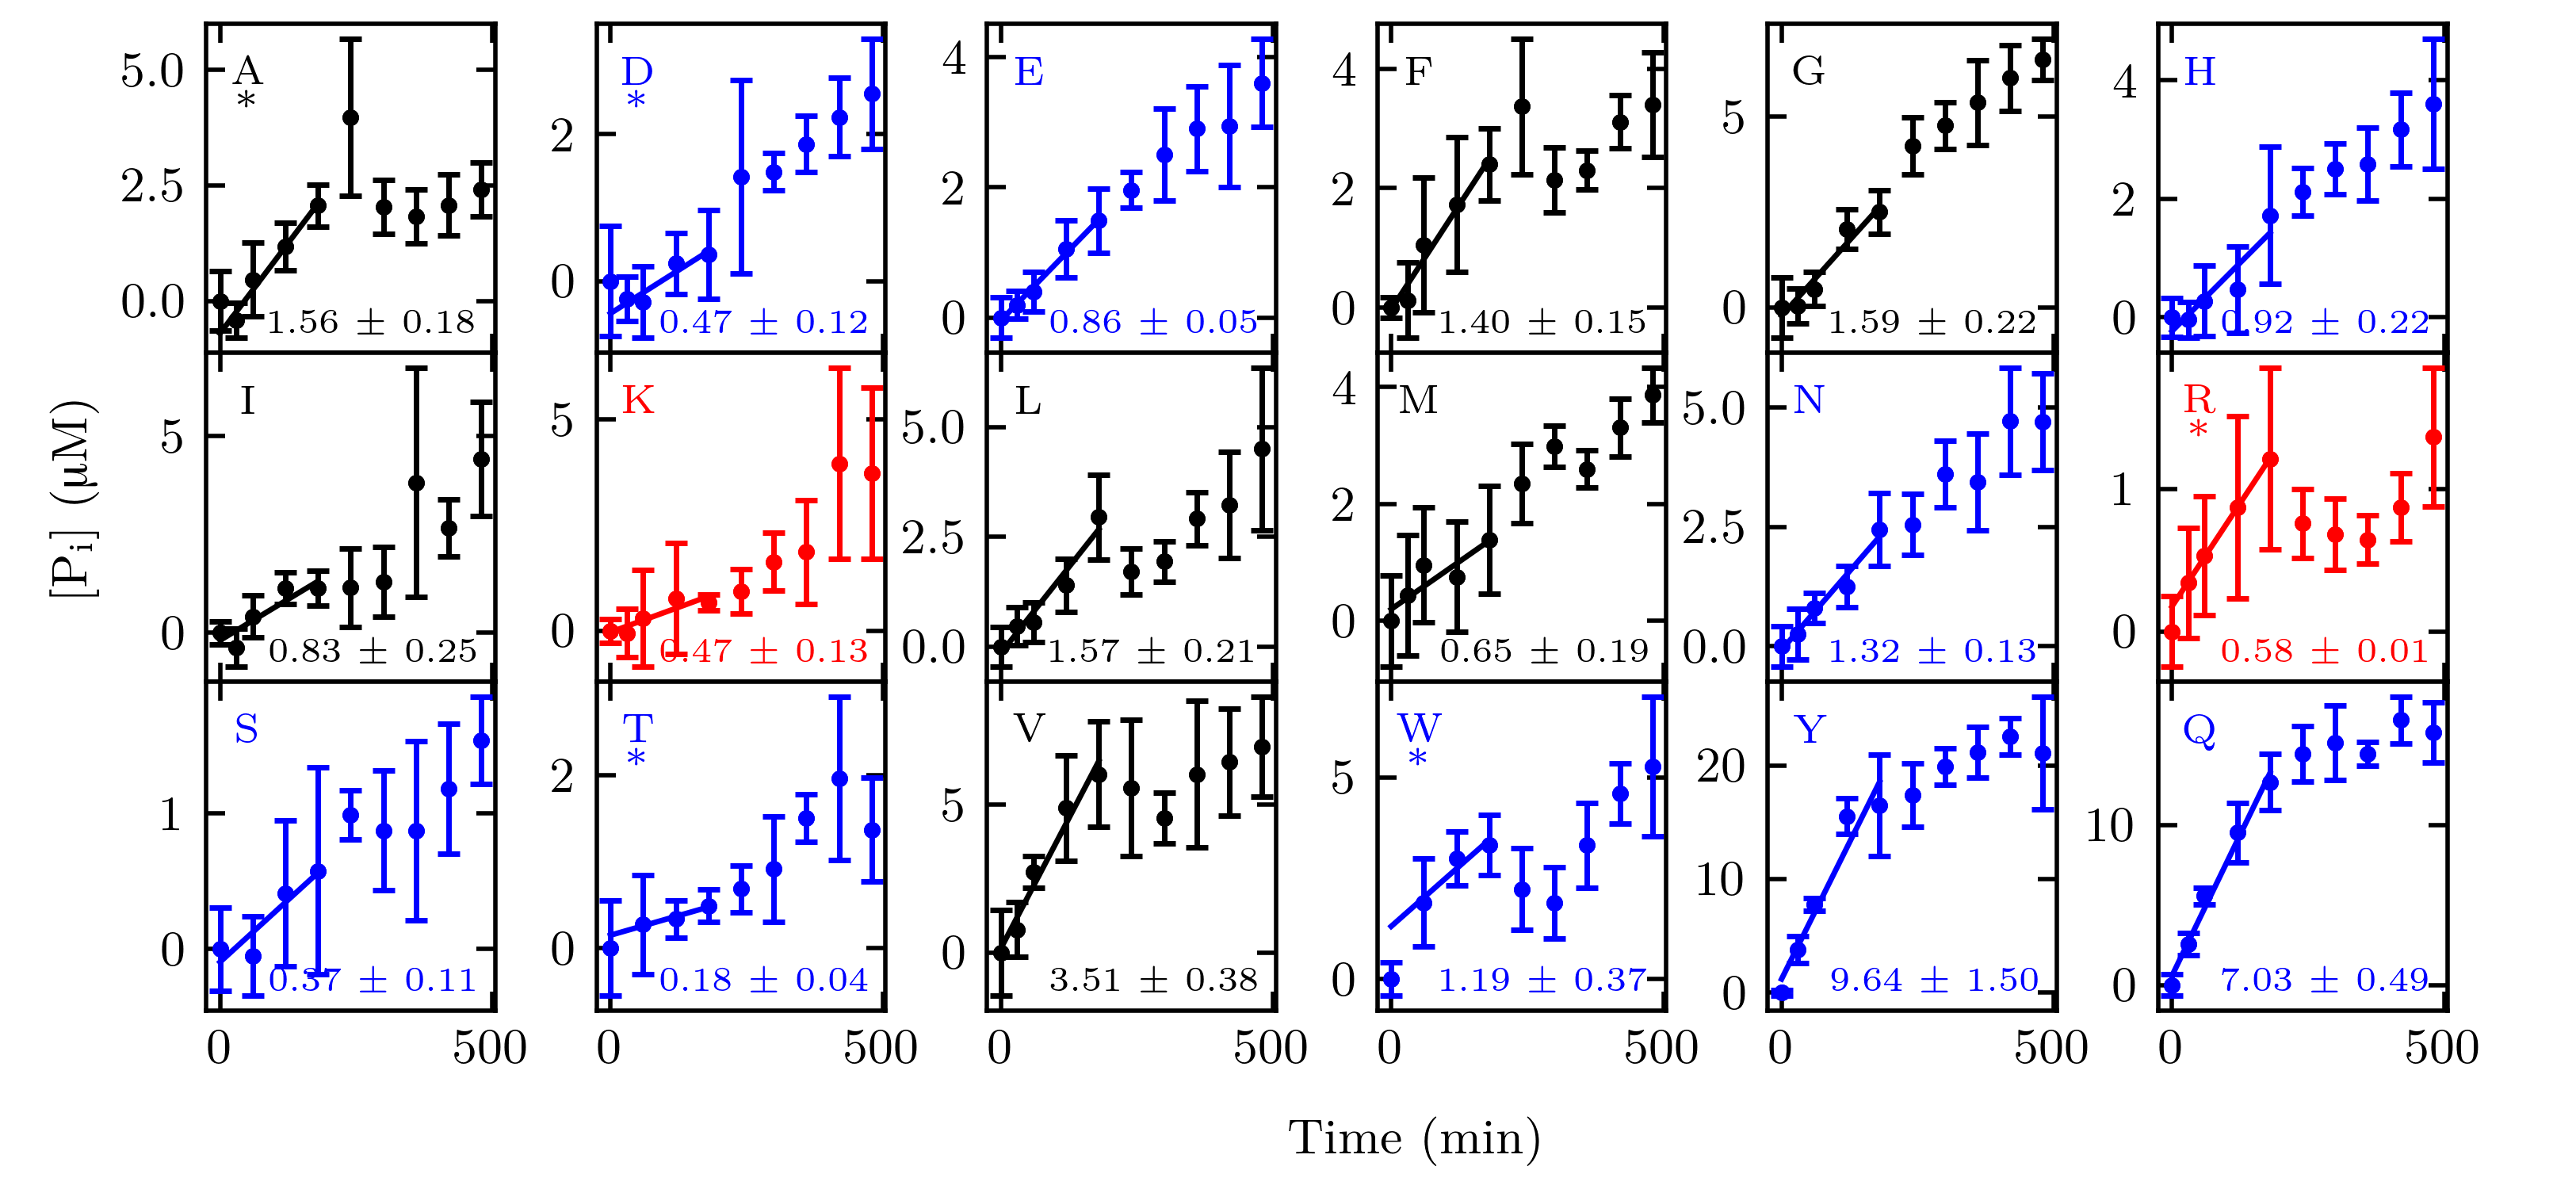
\includegraphics[width=\double]{figures-ras/all_fits.png}
    \caption{
        The production of inorganic phosphate, \ce{Pi}, as a function of reaction time for all viable RasQ61X constructs. 
        The identity of the amino acid at position 61 is shown in the upper left corner of each plot. 
        The first five points were fit with linear regression. 
        The slope and standard error of the fit are displayed in the bottom-right corner of each window. 
        If a lower standard error was obtained by omitting the first time point (0 min), then that fit is reported. 
        Such cases are marked with an asterisk in the top-left corner. 
        Blue: polar or negatively charged residues; red: positively charged residues; black: nonpolar residues.
    }
    \label{fig:ras-all_fits}
\end{figure}

\begin{table}
    \caption[Summary of experimental and computational results]{
        Vibrational Frequencies of a Nearby Nitrile on \RalBSCN{}, 
        Measured Intrinsic Initial Rates of GTP hydrolysis, and 
        Computed SASA Values of Both the Entire Side Chain and Only the Side Chain Polar Atoms (N, O, and H bound to N or O) from MD Simulation for 18 Constructs of RasQ61X
    }
    \begin{center}
    \begin{tabular}{ccccc}
    \toprule
    \rowcolor{lgray}
        Ras Construct & $\tilde{\nu}^{a}$   & Initial Rate$^{b}$  & \multicolumn{2}{c}{SASA$^{c}$ of: (\si{\angstrom^2}) }\\
    \rowcolor{lgray}
    & (cm$^{-1}$) &     ($10^{-2}$ $\mu$M min$^{-1}$)  & polar atoms & side chain \\
    \cmidrule(r){1-1}\cmidrule(lr){2-2}\cmidrule(lr){3-3}\cmidrule(l){4-5}
    WT Ras$^{d}$   & $2162.8 \pm 0.2$ & $ 7.03 \pm 0.49  $ & $65 \pm 15$ & $98  \pm 16 $\\
    \rowcolor{lgray}
    \multicolumn{5}{c}{Residues with Charged Sidechains} \\
    RasQ61D & $2162.0 \pm 0.1$ & $ 0.47 \pm  0.12 $ & $51 \pm 7  $ & $77  \pm 7  $\\
    RasQ61E & $2162.8 \pm 0.2$ & $ 0.86 \pm  0.05 $ & $60 \pm 10.$ & $91  \pm 11 $\\
    RasQ61K & $2163.1 \pm 0.2$ & $ 0.47 \pm  0.13 $ & $50 \pm 17 $ & $114 \pm 22 $\\
    RasQ61R & $2162.4 \pm 0.1$ & $ 0.58 \pm  0.01 $ & $71 \pm 24 $ & $121 \pm 24 $\\
    \rowcolor{lgray}
    \multicolumn{5}{c}{Residues with Polar Sidechains} \\
    RasQ61H & $2163.8 \pm 0.2$ & $ 0.92 \pm  0.22 $ & $34 \pm 6  $ & $108 \pm 14 $\\
    RasQ61N & $2162.7 \pm 0.2$ & $ 1.32 \pm  0.13 $ & $49 \pm 13 $ & $76  \pm 10 $\\
    RasQ61S & $2164.4 \pm 0.1$ & $ 0.37 \pm  0.11 $ & $18 \pm 9  $ & $47  \pm 9  $\\
    RasQ61T & $2164.7 \pm 0.2$ & $ 0.18 \pm  0.04 $ & $20 \pm 9  $ & $59  \pm 11 $\\
    RasQ61W & $2164.1 \pm 0.2$ & $ 1.19 \pm  0.37 $ & $18 \pm 10.$ & $151 \pm 21 $\\
    RasQ61Y & $2163.5 \pm 0.1$ & $ 9.64 \pm  1.50 $ & $36 \pm 15 $ & $130.\pm 25 $\\
    \rowcolor{lgray}
    \multicolumn{5}{c}{Residues with Nonpolar Sidechains} \\
    RasQ61A & $2162.0 \pm 0.2$ & $ 1.56 \pm  0.18 $ &                   &         \\
    RasQ61F & $2163.0 \pm 0.2$ & $ 1.40 \pm  0.15 $ & $0  \pm 0  $ & $114 \pm 21 $\\
    RasQ61G & $2163.1 \pm 0.1$ & $ 1.59 \pm  0.22 $ &              &              \\
    RasQ61I & $2164.0 \pm 0.2$ & $ 0.83 \pm  0.25 $ & $0  \pm 0  $ & $95  \pm 9  $\\      
    RasQ61L & $2163.2 \pm 0.2$ & $ 1.57 \pm  0.21 $ & $0  \pm 0  $ & $102 \pm 14 $\\
    RasQ61M & $2162.6 \pm 0.1$ & $ 0.65 \pm  0.19 $ & $0  \pm 0  $ & $101 \pm 20 $\\
    RasQ61V & $2163.9 \pm 0.0$ & $ 3.51 \pm  0.38 $ & $0  \pm 0  $ & $78  \pm 11 $\\
    \bottomrule
    \end{tabular} \\
    \end{center}
    $^{a}$Taken from ref \citenum{Stafford2012}. $^{b}$Errors in the rate are reported as the standard error of the linear fit. $^{c}$Errors in the SASA are reported as the standard deviation of the entire ensemble of structures. $^{d}$The identity of position 61 in wild-type Ras is Q.
    \label{tbl:ras-data}
\end{table}

\begin{figure}
    \center
    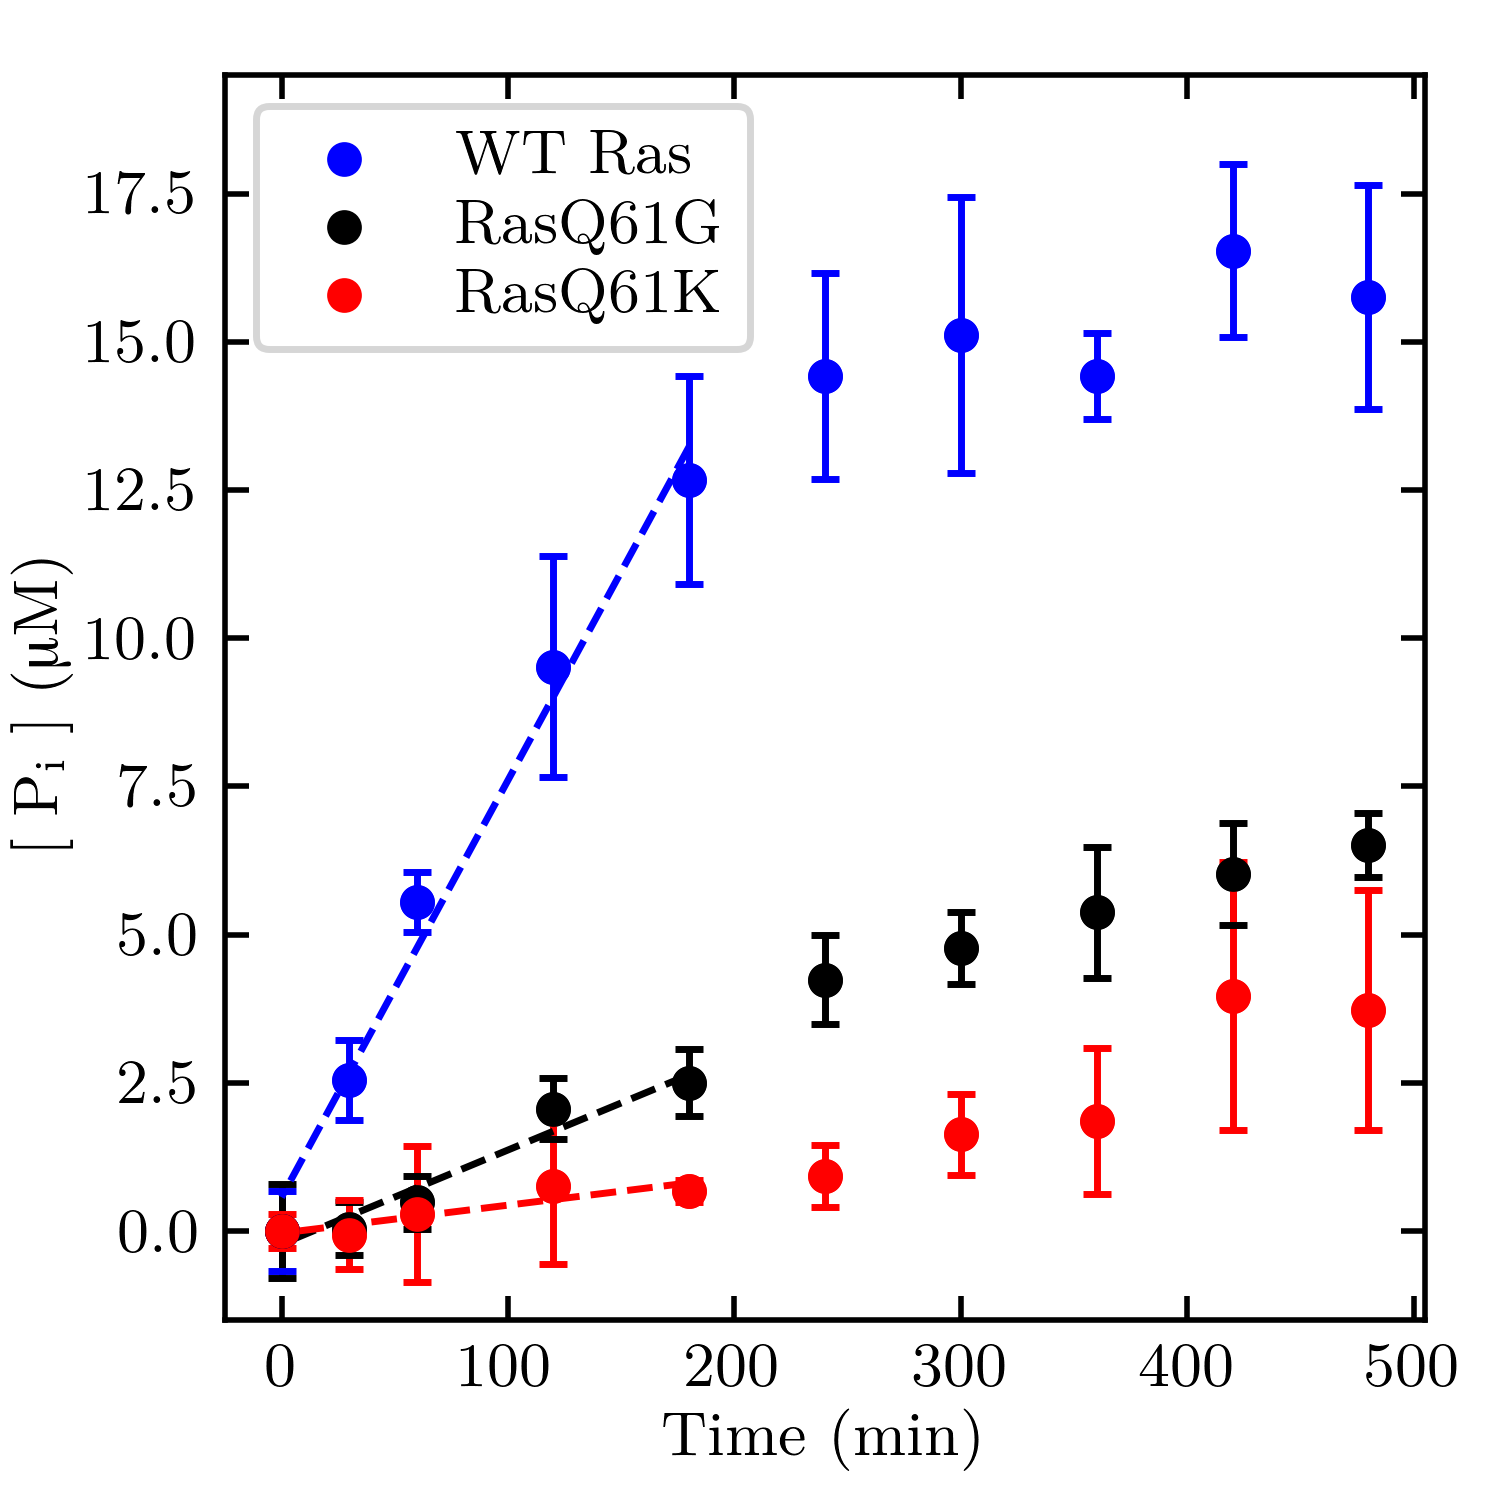
\includegraphics[width=\single]{figures-ras/modelCurvesFigure.png}
    \caption{
        Representative kinetic measurements of 4 $\mu$M RasQ61X constructs reacted with 20 $\mu$M GTP over 8 h, WT (blue), Q61G (black), and Q61K (red). 
        The dashed lines represent the linear fit to the first five time points. 
        The slope of the linear fit is the initial rate of the intrinsic hydrolysis reaction. 
        The rates for each mutant are reported in Table \ref{tbl:ras-data}.}
    \label{fig:ras-curves}
\end{figure}

Though the most common approach to enzyme kinetics is the Michaelis-Menten formalism \cite{Michaelis1913, Johnson2011}, in this case, the mutations at position 61 should affect the turnover rate of the enzyme ($k_{\text{cat}}$) and not the overall Michaelis constant ($K_m$). 
Because of this, measuring the initial rate at a single substrate concentration was sufficient, given the number of constructs we investigated. 
Because initial rates depend on a variety of conditions including protein and substrate concentrations, buffer conditions, and temperature, all constructs were measured under exactly the same conditions, so they could be compared appropriately. 
In general, our results corroborate previously reported qualitative results that Q61X mutants tend to have significantly lower rates of intrinsic GTP hydrolysis with one notable exception: Q61Y had a faster initial rate ($9.64 \pm 1.50 \times 10^{-2}$ $\mu$M min$^{-1}$) than the WT ($7.03 \pm 0.49 \times 10^{-2}$ $\mu$M min$^{-1}$). 
However, all other Q61X mutant rates were slower than WT. 
Q61V had a moderate hydrolysis rate of $3.51 \pm 0.38 \times 10^{-2}$ $\mu$M min$^{-1}$. 
However, this construct precipitated after 3 h, suggesting that while the initial rate was faster than other mutations, the protein was less stable. 
The other 14 mutants we measured had initial rates of intrinsic GTP hydrolysis of less than $2.00 \times 10^{-2}$ $\mu$M min$^{-1}$.

In order to understand these results, we sorted the mutants into categories based on the polarity and ionizability of the side chain at position 61, factors which are expected to be significant for the ability to interact with and stabilize any catalytically important water molecules in the active site. 
Residues with positively charged side chains (K and R) had measured initial rates between $0.40 \times 10^{-2}$ and $0.60 \times 10^{-2}$ $\mu$M min$^{-1}$, a 15-fold decrease in intrinsic rate from WT. 
Residues with negatively charged side chains (D and E) had measured initial rates between $0.40$ and $0.90 \times 10^{-2}$ $\mu$M min$^{-1}$, a 10- to 20-fold decrease. 
For the nonpolar residues (A, F, G, I, L, M, and V), we measured initial rates between $0.6 \times 10^{-2}$ and $1.6 \times 10^{-2}$ $\mu$M min$^{-1}$, with the exception of V for which we measured a rate of $3.51 \times 10^{-2}$ $\mu$M min$^{-1}$. 
Polar, uncharged residues (H, N, Q, S, T, W, and Y) varied much more significantly, the fastest of which were the WT (Q) measured at $7.03 \times 10^{-2}$ $\mu$M min$^{-1}$ and Y measured at $9.64 \times 10^{-2}$ $\mu$M min$^{-1}$.
Two of the larger polar residues (H and W) had measured rates of $0.92 \times 10^{-2}$ $\mu$M min$^{-1}$ and $1.19 \times 10^{-2}$ $\mu$M min$^{-1}$, respectively. 
The smaller polar residues (S and T) were among the slowest mutants with rates of $0.37 \times 10^{-2}$ $\mu$M min$^{-1}$ and $0.18 \times 10^{-2}$ $\mu$M min$^{-1}$, respectively. 
The remaining large polar mutant (N), which is the most chemically similar to the wild-type Q, had a rate of $1.32 \times 10^{-2}$ $\mu$M min$^{-1}$, approximately six times slower than the WT rate. 
Although the few published rate constants of intrinsic hydrolysis by RasQ61X mutants reported in the literature have been calculated using the Michaelis-Menten formalism, and therefore cannot be compared directly to our initial rate measurements, we report them here for convenience. 
John et al. reported rate constants of $2.8 \times 10^{-2}$ min$^{-1}$ for the WT Ras and $0.2 \times 10^{-2}$ min$^{-1}$ for RasQ61H \cite{John1988}. 
Krengel et al. reported an observed rate of $0.1 \times 10^{-2}$ min$^{-1}$ for RasQ61L \cite{Krengel1990}.
RasQ61E has been reported to have a 10-fold slower hydrolysis rate than the WT\cite{Der1986}; however, Frech et al. reported a 20-fold faster intrinsic hydrolysis rate for RasQ61E when controlling for the 100-fold larger $K_d$ values for the RasQ61E-GTP complex \cite{Frech1994}.

Recently, Stafford et al. used VSE spectroscopy to measure electric field changes due to the change in identity of the residue at RasQ61\cite{Stafford2012}. 
In those experiments, RasQ61X was docked to \RalBSCN{}, which contained a cyanocysteine vibrational probe. 
The FTIR absorption frequencies from the nitrile group on the probe when docked to each Ras mutant are listed in Table \ref{tbl:ras-data}. 
Though \RalB{} docks to GTP-bound Ras with a micromolar $K_d$, we did not expect it to have an effect on the Ras intrinsic hydrolysis rate. 
To confirm this, and in order to compare our rate results with the published VSE data, we measured the intrinsic hydrolysis rate of WT Ras alone versus WT Ras docked to \RalBSCN{} and observed no differences in the rate of intrinsic hydrolysis whether or not \RalBSCN{} was present (Figure \ref{fig:ras-ral}).

\begin{figure}
    \center
    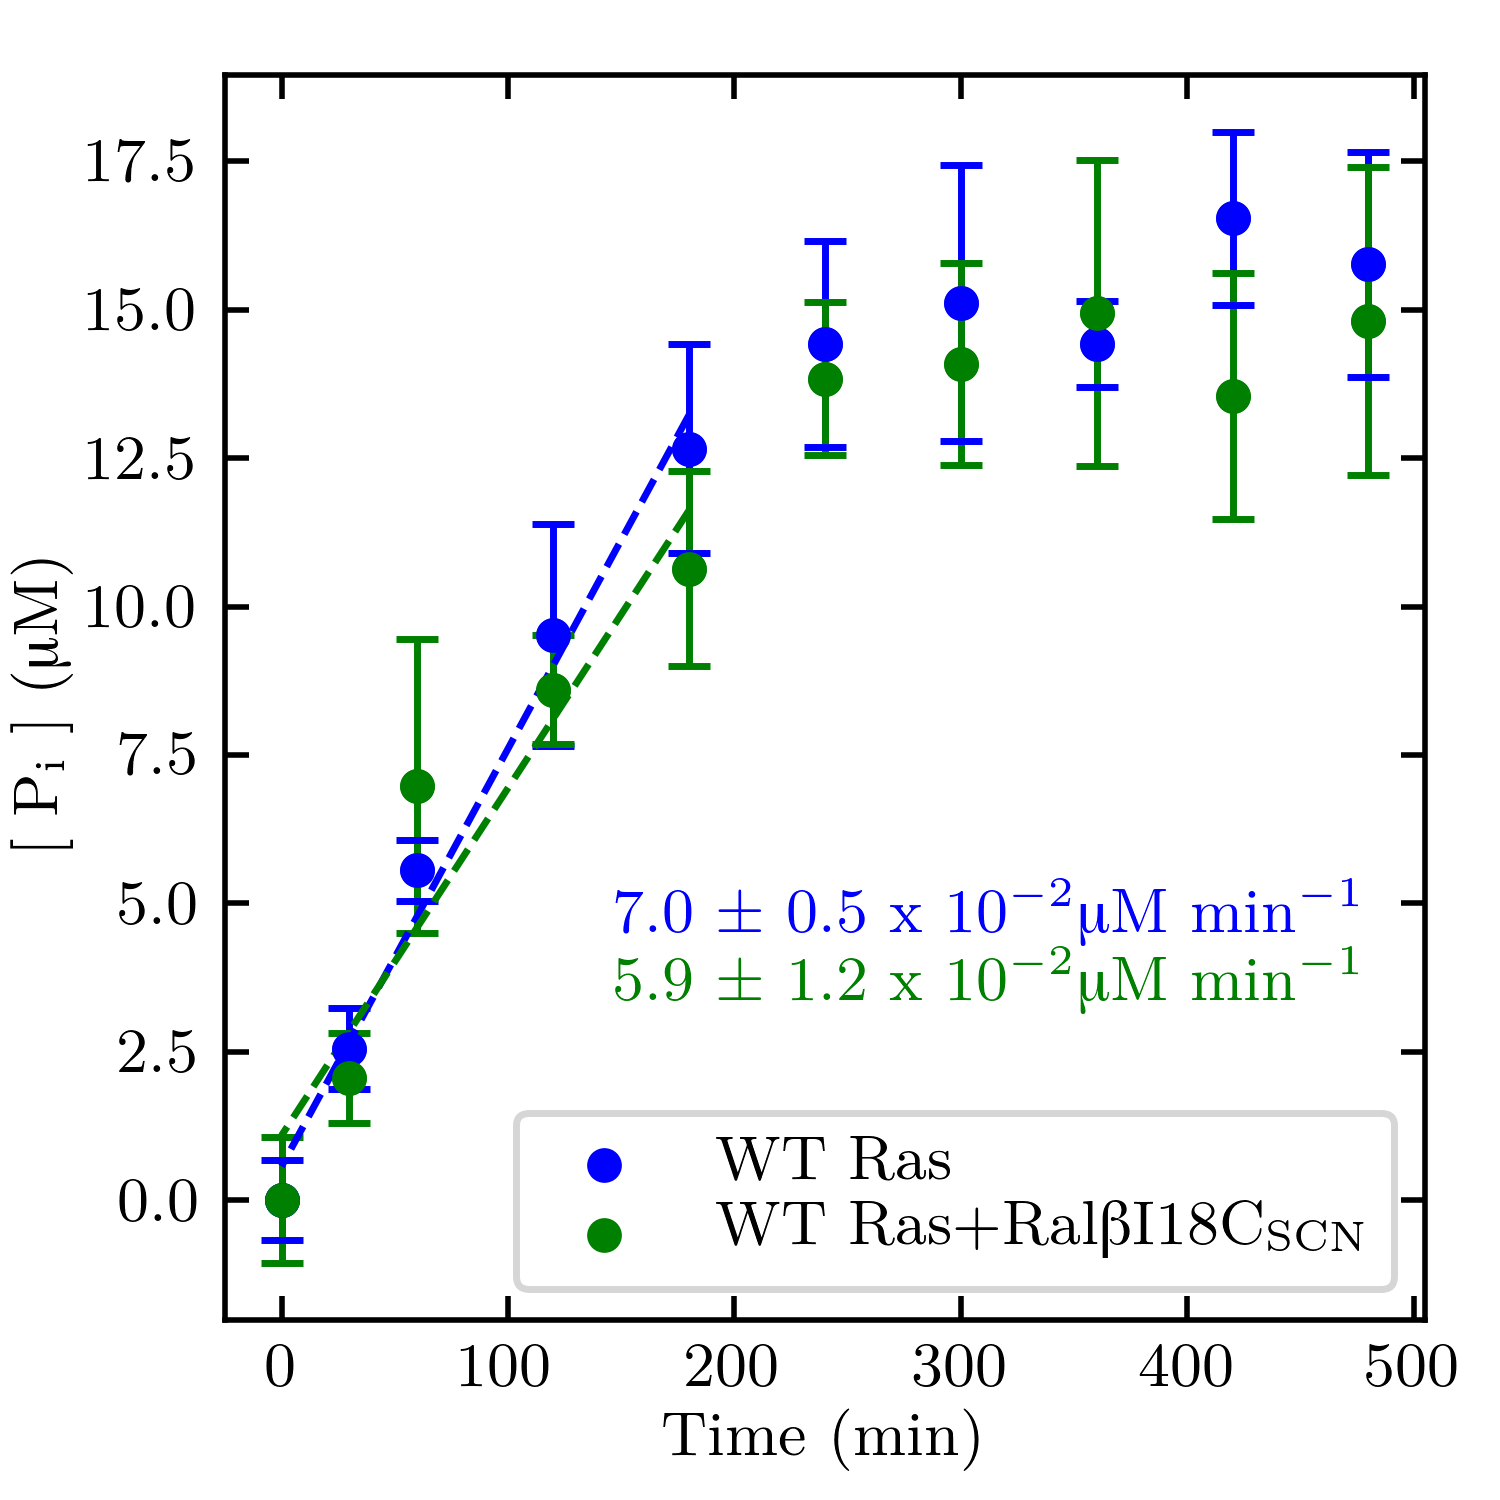
\includegraphics[width=\single]{figures-ras/Figure3.png}
    \caption{
        Concentration of the phosphate product of the intrinsic hydrolysis reaction for both WT Ras (blue) and WT Ras docked to \RalBSCN{} (green) over 8 h. 
        Linear regression fits are shown to the first five time points of each data set, and the slopes are displayed in the corresponding color. 
        The intrinsic hydrolysis rate of WT Ras/\RalBSCN{} is within error of the intrinsic hydrolysis rate of WT Ras alone ($5.9 \pm 1.1 \times 10^{-2}$ $\mu$M min$^{-1}$ and $7.0 \pm 0.5 \times 10^{-2}$ $\mu$M min$^{-1}$, respectively).
    }
    \label{fig:ras-ral}
\end{figure}

\subsection{SASA Calculations}

Because the proposed mechanism in Figure \ref{fig:ras-mech}A is based on a favorable interaction of Q61 with water, we attempted to quantify the likelihood of this interaction by calculating the SASA for each mutant of several subsets of atoms of the Q61X residue using the gmx sasa tool \cite{Eisenhaber1995}.
While SASA is often an oversimplification of solvent interactions, it is nevertheless a good starting point because it is efficient and convenient to calculate from a protein structure or MD trajectory. 
We therefore calculated the SASA of both the whole side chain and the polar atoms on the side chain; we refer to these quantities as the ``side chain SASA'' and the ``polar atom SASA,'' respectively. 
All N and O atoms and their bonded hydrogens were considered to be polar atoms. 
Each calculated SASA was weighted using the weighted histogram analysis method (WHAM) at 300 K, and the Boltzmann-weighted average SASA value was computed. 
These averages and standard deviations are reported in Table \ref{tbl:ras-data}.

Since F, I, L, M, and V do not have polar atoms on their side chains, the polar atom SASAs for these residues were exactly zero. 
S, T, and W all had similar polar atom SASAs of $\sim$18 \si{\angstrom^2}. 
This is not surprising, since they each have one heavy polar atom and one polar hydrogen. 
However, Y, which also has one polar heavy atom and one polar hydrogen, had a polar atom SASA of $\sim$37 \si{\angstrom^2}, more than double the other hydroxyl side chains (S and T), suggesting that the polar atoms of Y interact much more strongly with water than S or T. 
H, which has two polar heavy atoms but only one polar hydrogen, had a similar polar atom SASA of $\sim$34 \si{\angstrom^2}. 
The other two polar, uncharged residues (N and Q) have identical polar groups yet exhibited different polar atom SASAs at $\sim$49 \si{\angstrom^2} and $\sim$65 \si{\angstrom^2}. 
Similarly, the two negatively charged residues (D and E) have identical polar groups yet exhibited different polar atom SASAs at $\sim$51 \si{\angstrom^2} and $\sim$60 \si{\angstrom^2}, respectively. 
In both of these cases (N versus Q, and D versus E), the larger residue had the larger polar SASA, indicating the extra carbon in the side chain allowed the polar atoms to extend further from the backbone and interact more with solvent. 
Finally, we calculated a polar atom SASA for K that was similar to that of N and D ($\sim$50 \si{\angstrom^2}), and we calculated the largest polar atom SASA for R (which has the most polar atoms) of $\sim$71 \si{\angstrom^2}.

We also calculated the side chain SASAs for all mutants and compared them to the polar atom SASAs. 
Unsurprisingly, because of their relative size, S and T had the lowest side chain SASAs at $47 \pm 9$ \si{\angstrom^2} and $59 \pm 11$ \si{\angstrom^2},respectively. 
D, N,and V all had similar side chain SASAs at $77 \pm 7$ \si{\angstrom^2}, $76 \pm 10$ \si{\angstrom^2}, and $78 \pm 11$ \si{\angstrom^2}, respectively, despite D and T having about the same molecular volume.
This indicates that the polar side chain of T spent more time interacting with the protein than D, and less time interacting with water. 
Residues M, L, E, I, and Q all had intermediate side chain SASAs that fell between 91 \si{\angstrom^2} and 101 \si{\angstrom^2}. 
Residues F, H, K, and R had larger side chain SASAs at $114 \pm 21$ \si{\angstrom^2}, $108 \pm 14$ \si{\angstrom^2}, $114 \pm 22$ \si{\angstrom^2},and $121 \pm 24$ \si{\angstrom^2}, respectively. 
This is surprisingly low for R, indicating that the positively charged side chain interacted favorably with the surrounding protein but not available water molecules.
Finally, residues W and Y had the largest side chain SASA values at $151 \pm 21$ \si{\angstrom^2} and $130 \pm 25$ \si{angstrom^2}. 
While such a large value is unsurprising for W since the residue is so large, 130 \si{\angstrom^2} is nearly the maximum surface area for Y, indicating a very favorable interaction with the solvent environment. 
Combined, the SASA calculations indicated that residues similar in size and chemical identity can still partition differently in water based on the local chemical structure of the protein near position 61 and therefore make different contributions both to the electric field and the distribution of water in the active site. 

%%%%%%%%%%%%%%%%%%%%%%%%%%%%%%%%%%%%%%%%%%%%%%%%%%%%%%%%%%%%%%%%
%%%%%%%%%%%%%%%%%%%%%%%%%%%%%%%%%%%%%%%%%%%%%%%%%%%%%%%%%%%%%%%%
\section{Discussion}\label{ras-discussion}
%%%%%%%%%%%%%%%%%%%%%%%%%%%%%%%%%%%%%%%%%%%%%%%%%%%%%%%%%%%%%%%%
%%%%%%%%%%%%%%%%%%%%%%%%%%%%%%%%%%%%%%%%%%%%%%%%%%%%%%%%%%%%%%%%

Because the proposed mechanism of intrinsic hydrolysis of GTP in Ras (Figure \ref{fig:ras-mech}A) relies on electrostatic stabilization of a transient hydronium ion in the active site, we plotted the measured vibrational frequencies from Stafford et al.\cite{Stafford2012} against the measured initial rates of intrinsic hydrolysis (Figure \ref{fig:ras-stark_vs_rate}). 
Since hydrolysis rates change by nearly 2 orders of magnitude, it is useful to view these differences in rate on a logarithmic scale. 
For the polar and negatively charged residues, which are capable of stabilizing the proposed hydronium ion, the rates increased rapidly with increasing nitrile absorption frequency until $\sim$2163 \si{\wn}, the absorption energies of Ras containing both Q (i.e., WT) and Y at position 61, and then rapidly decreased with the continued increase in absorption frequency. 
This correlation was fit to a normal distribution with the residues capable of stabilizing the hydronium ion (the polar and negatively charged residues). 
For these data, residues that caused the nitrile absorption frequency to red-shift or blue-shift from $\sim$2163 \si{\wn} decreased the rate.

\begin{figure}
    \center
    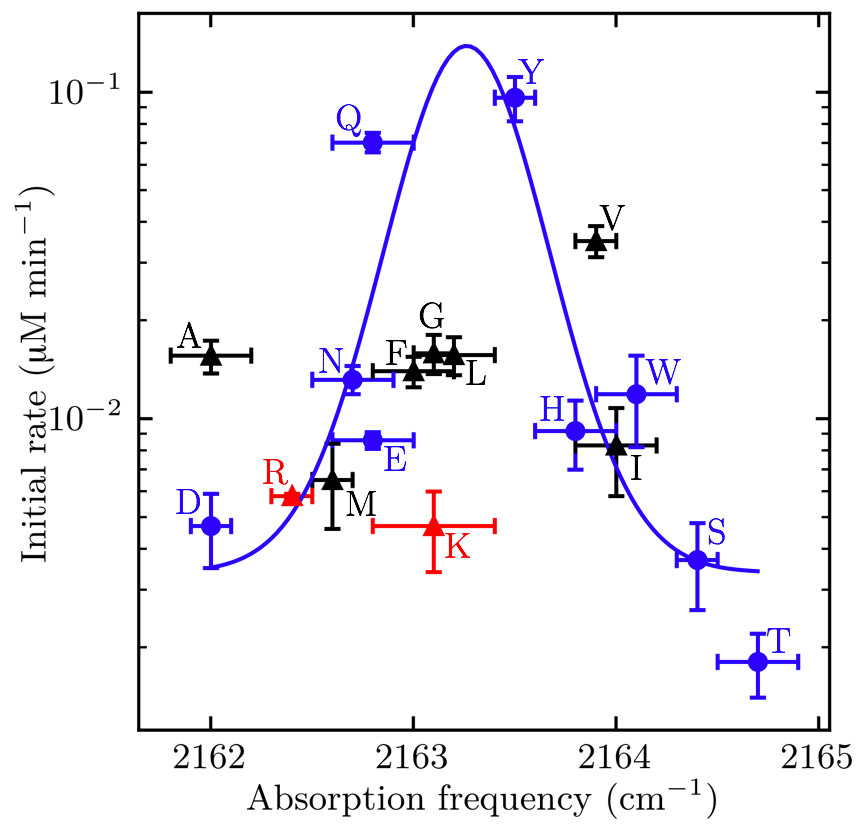
\includegraphics[width=\single]{figures-ras/Figure4.png}
    \caption{
        Vibrational frequencies of the nitrile on \RalBSCN{} against the log of the measured intrinsic rate of GTP hydrolysis. 
        Blue: polar and negatively charged side chains. Black: all nonpolar side chains. 
        Red: the two positively charged side chains. Blue line: normal distribution fit to the polar and the negatively charged side chains. 
        All points that were excluded from the fit are marked with triangles.
    }
    \label{fig:ras-stark_vs_rate}
\end{figure}

Because nitrile groups have been shown to report on changes in solvation due to hydrogen bonding, we calculated the SASA of the nitrile on \RalBSCN{} and the number of waters within a 5 \si{\angstrom} sphere of the nitrile. 
These values were within error of each other for all of the Q61X mutants and are presented in Table \ref{tbl:ras-sasa}. 
Further, because the solvation effect is caused by changes in specific hydrogen bonding interactions\cite{Choi2008}, we calculated the geometries of each observed hydrogen bond between the nitrile and solvent. 
Recently, we have shown that the geometry of these interactions can dominate the vibrational frequency\cite{First2018}.
In this case, however, the average angles and distances of the hydrogen bonding interactions were all within error of each other for each of the 18 mutant systems, as shown in Table \ref{tbl:ras-sasa}. 
Together, these data demonstrate that the perturbation to the solvation environment caused by the mutation has relaxed over the $\sim$9 \si{\angstrom} distance between the nitrile probe and position 61. 
We have previously demonstrated that, in cases of a similar hydrogen bonding environment, such as these systems, shifts in nitrile frequency agree with independent measurements of electric field \cite{Slocum2016, Slocum2017}.
We therefore interpret the shifts in absorption frequency as a measure of change in the electric field through eq \ref{eq:ras-stark}.

\begin{table}
    \caption[Nitrile exposure to water in the Ras/\RalBSCN{} constructs]{
        Boltzmann-weighted averages of the SASA of the nitrile on \RalBSCN{}, 
        number of waters within a 5 \si{\angstrom} sphere of the nitrogen of the nitrile, and 
        geometric properties of all the hydrogen bonding interaction between the solvent and the nitrile in the simulations. 
        These geometric properties are illustrated in Figure \ref{fig:ras-hbond}.
    }
    \begin{center}
    \begin{tabular}{cccccc} 
    \toprule
        \rowcolor{lgray}
        Ras Construct & SASA (\si{\angstrom^2})  & \# waters & $\left < \theta_1 \right >$  & $\left < \theta_2 \right >$ & $\left < d_{\rm{NH}} \right >$ (\si{\angstrom}) \\
    
        \cmidrule(r){1-1}\cmidrule(lr){2-2}\cmidrule(lr){3-3}\cmidrule(lr){4-4}\cmidrule(lr){5-5}\cmidrule(l){6-6}
    
    RasQ61D  & $51 \pm 13$  &  $14 \pm 2$    &  $135.2 \pm 19.3$ & $152.3 \pm 13.5$  & $2.1 \pm 0.2 $              \\  
    RasQ61E  & $60 \pm 13$  &  $15 \pm 2$    &  $133.5 \pm 19.3$ & $152.2 \pm 13.6$  & $2.1 \pm 0.2 $              \\  
    RasQ61F  & $51 \pm 17$  &  $14 \pm 3$    &  $137.3 \pm 19.4$ & $153.2 \pm 13.1$  & $2.1 \pm 0.2 $              \\  
    RasQ61H  & $48 \pm 15$  &  $14 \pm 3$    &  $137.4 \pm 19.3$ & $152.9 \pm 13.4$  & $2.1 \pm 0.2 $              \\  
    RasQ61I  & $58 \pm 15$  &  $15 \pm 3$    &  $134.6 \pm 18.9$ & $152.6 \pm 13.5$  & $2.1 \pm 0.2 $              \\  
    RasQ61K  & $56 \pm 16$  &  $15 \pm 3$    &  $135.1 \pm 19.6$ & $152.9 \pm 13.2$  & $2.1 \pm 0.2 $              \\  
    RasQ61L  & $57 \pm 17$  &  $15 \pm 3$    &  $135.5 \pm 18.8$ & $153.1 \pm 13.6$  & $2.1 \pm 0.2 $              \\  
    RasQ61M  & $48 \pm 18$  &  $13 \pm 3$    &  $136.9 \pm 19.3$ & $153.3 \pm 13.0$  & $2.1 \pm 0.2 $              \\  
    RasQ61N  & $52 \pm 17$  &  $14 \pm 3$    &  $135.1 \pm 19.3$ & $152.3 \pm 13.6$  & $2.1 \pm 0.2 $              \\  
    RasQ61Q  & $55 \pm 19$  &  $14 \pm 3$    &  $137.2 \pm 19.1$ & $153.0 \pm 13.3$  & $2.1 \pm 0.2 $              \\  
    RasQ61R  & $61 \pm 19$  &  $15 \pm 3$    &  $135.3 \pm 19.1$ & $152.7 \pm 13.5$  & $2.1 \pm 0.2 $              \\  
    RasQ61S  & $53 \pm 16$  &  $13 \pm 3$    &  $132.0 \pm 18.6$ & $152.6 \pm 13.7$  & $2.1 \pm 0.2 $              \\  
    RasQ61T  & $45 \pm 19$  &  $13 \pm 3$    &  $134.8 \pm 19.6$ & $152.7 \pm 13.7$  & $2.1 \pm 0.2 $              \\  
    RasQ61V  & $53 \pm 17$  &  $15 \pm 3$    &  $136.9 \pm 19.3$ & $153.7 \pm 13.1$  & $2.1 \pm 0.2 $              \\  
    RasQ61W  & $62 \pm 15$  &  $15 \pm 3$    &  $136.3 \pm 18.9$ & $151.8 \pm 13.7$  & $2.1 \pm 0.2 $              \\  
    RasQ61Y  & $56 \pm 18$  &  $14 \pm 3$    &  $135.8 \pm 19.0$ & $152.4 \pm 13.5$  & $2.1 \pm 0.2 $              \\  
    
    \bottomrule
    \end{tabular}
    \end{center}
    \label{tbl:ras-sasa}
\end{table}

\begin{figure}
    \center
    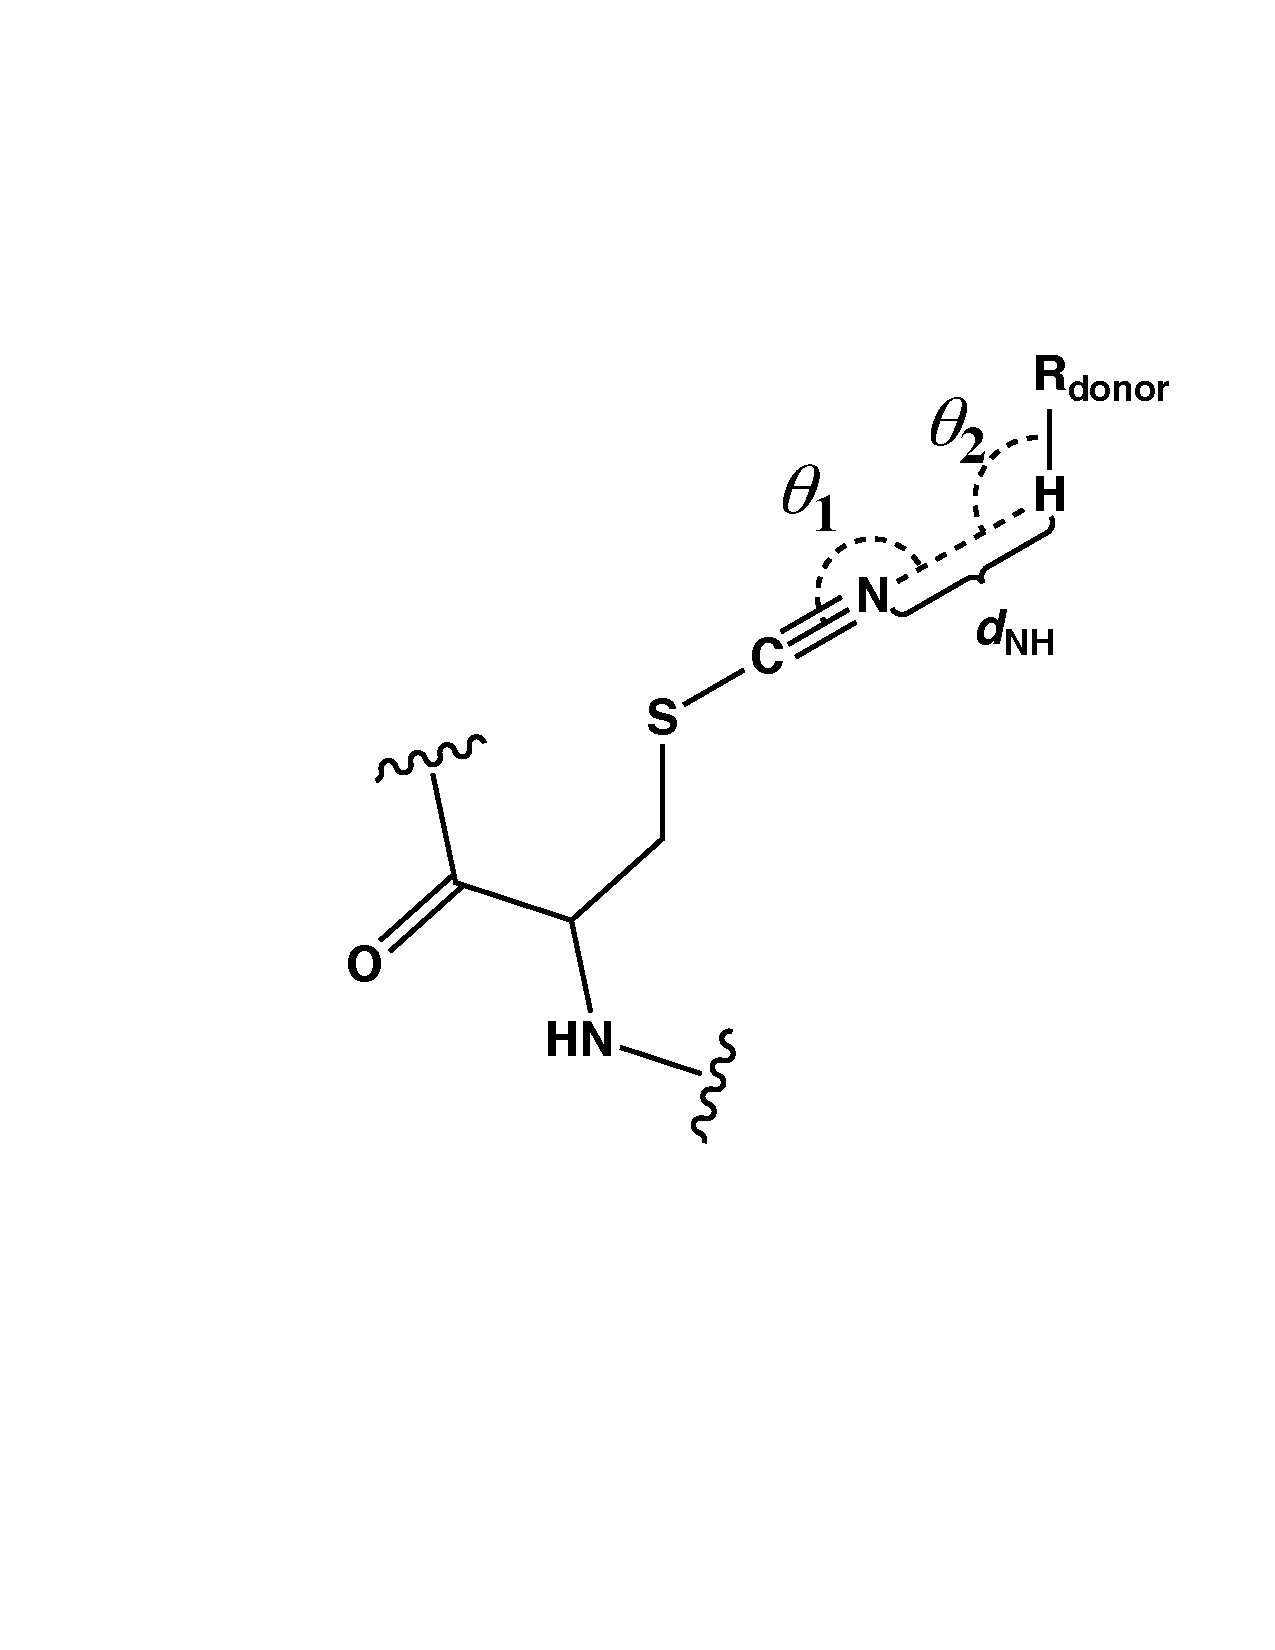
\includegraphics[width=\single]{figures-ras/Figure_S4.pdf}
    \caption{
        Geometric criteria and property definitions for the hydrogen bonding calculations. 
        $\theta_1$ is the C--N$\cdots$H angle, $\theta_2$ is the N$\cdots$H--R$_{\text{donor}}$ angle, where R$_{\text{donor}}$ represents a water hydrogen bond donor, and $d_{\text{NH}}$ is the distance between the hydrogen and the acceptor nitrogen. 
        To be considered a hydrogen bond, $\theta_1$ must be greater than \ang{99}, $\theta_2$ must be greater than \ang{120}, and $d_{\text{NH}}$ must be less than 2.45 \si{\angstrom}. 
        Adopted from ref \citenum{First2018}.
    } 
    \label{fig:ras-hbond}
\end{figure}

The observation in Figure \ref{fig:ras-stark_vs_rate} supports the hypothesis that the role of Q61 is to provide an electrostatic contribution to the stabilization of water near the active site and that Q61X mutants that do not provide the optimal electrostatic potential; i.e., all mutants studied besides Q and Y are less effective at stabilizing the catalytic hydronium ion. 
Mutations that caused a deviation from the optimal field in either direction (measured as a red- or blue-shift in the nitrile vibrational frequency) disrupted the intrinsic mechanism and decreased the rate, except for residues that did not stabilize a hydronium ion, resulting in rates that are normally distributed about an optimal electric field.

For the residues that would be unable to stabilize the hydronium ion in the active site, no such trend was observed. 
Two of the uncorrelated residues are R and K, the two positively charged amino acids (red data points in Figure \ref{fig:ras-stark_vs_rate}). 
These two side chains are incapable of stabilizing a hydronium ion due to Coulombic repulsion and are thus easily explained. 
The hydrophobic residues at position 61 display a more interesting behavior, however, with a range of hydrolysis activities depending on the identity of the hydrophobic residue (black data points in Figure \ref{fig:ras-stark_vs_rate}). 
For example, V has an intermediate initial rate of intrinsic hydrolysis ($3.51 \pm 0.38$ $\mu$M min$^{-1}$), while M has a very low initial rate ($0.65 \pm 0.19$ $\mu$M min$^{-1}$).  
Side chain size alone does not explain this observation: G, A, V, and L increase in molecular volume in that order, but the rates of GTP hydrolysis in those Q61X mutants do not follow the same trend.

In order to investigate the effect of side chain size, we plotted the polar atom SASA and the side chain SASA for each mutant against the nitrile shift and the initial rate of GTP hydrolysis. 
As observed in Stafford et al., the SASA of the polar atoms are well correlated with the measured vibrational frequency of the nearby nitrile on \RalBSCN{} (Figure \ref{fig:ras-sasa}A). 
With increased sampling and increased accuracy of the SASA calculation, our correlation ($r = -0.89$) is improved compared to the previous result \cite{Stafford2012}. 
Therefore, the measured field observed by the nitrile is a good measure of the ability of Q61X to interact with water and thus a good metric by which to evaluate the hypothesis of Buhrman et al. 
No correlation was observed between the polar atom SASA and the measured intrinsic rate (Figure \ref{fig:ras-sasa}B), and when we measured the side chain SASA, we found that it did not correlate to the nitrile shifts (Figure \ref{fig:ras-sasa}C). 
However, we found that the SASA of the side chain was moderately correlated (Figure \ref{fig:ras-sasa}D, $r = 0.81$) to the measured initial rate of the side chains capable of stabilizing the hydronium ion (the polar and negatively charged residues), with the exception of W. 
Because of the unique chemical structure of W, the side chain SASA was extremely large, yet the large SASA of W did not translate to a large number of water molecules in the active site of the protein. 
This prompted us to calculate how many water molecules were actually present in the GTP binding site based on the identity of the residue at position 61.

\begin{figure}
    \center
    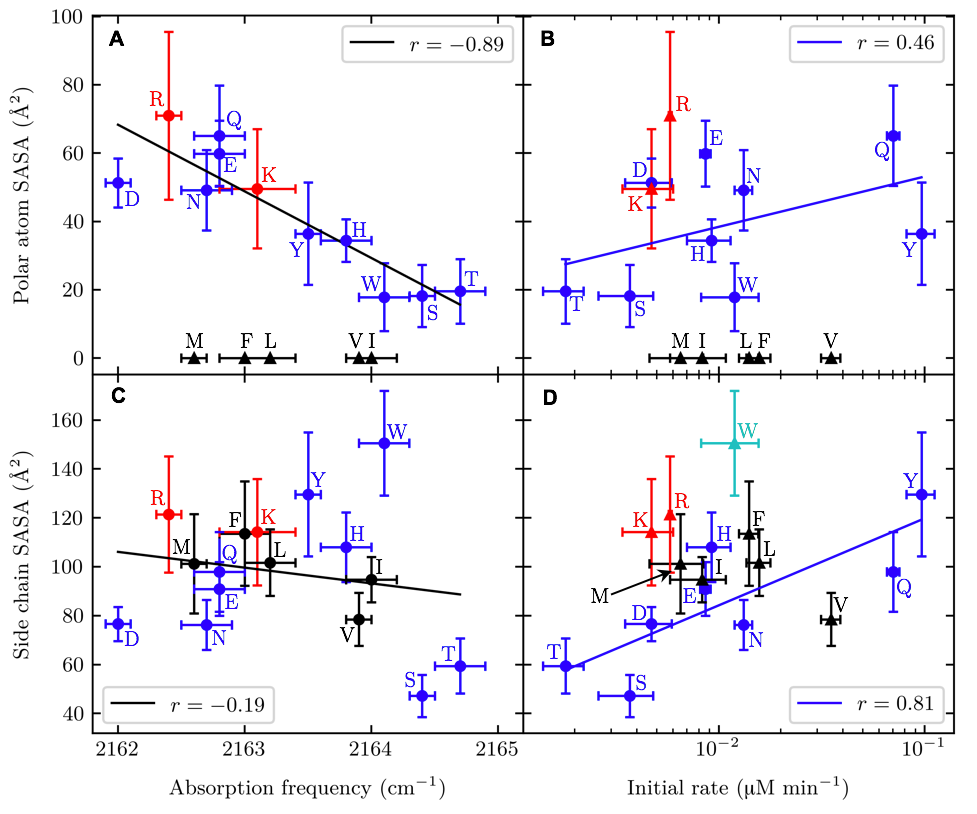
\includegraphics[width=\double]{figures-ras/Figure5.png}
    \caption{
        Boltzmann-weighted polar atom and side chain SASAs compared to experimentally measured values of nitrile absorption frequency and initial rate of intrinsic hydrolysis in RasQ61X mutants. 
        (A) The absorption frequency of the nitrile on \RalBSCN{} against the polar atom SASA of Q61X. 
        (B) The initial rate of intrinsic hydrolysis against the polar atom SASA of Q61X. 
        (C) The absorption frequency of the nitrile on \RalBSCN{} against the side chain SASA of Q61X. 
        (D) The initial rate of intrinsic hydrolysis against the side chain SASA of Q61X. 
        Blue: polar or negatively charged side chain. 
        Red: positively charged side chains. 
        Black: nonpolar side chains. 
        Triangles: residues not included in the linear regression. 
        In panel D, W (cyan) is excluded from the polar residue group as discussed in the text.
    }
    \label{fig:ras-sasa}
\end{figure}

While SASA is a convenient measure of the ability of a residue to interact with water, it lacks molecular level details of the interaction. 
Specifically, it does not address how much solvent is actually interacting with the residue. 
Instead, it only estimates the area of a residue that could interact with solvent. 
Because of this distinction and the observation that W interacted with a small number of waters, we calculated the number of waters that are confined to the active site around GTP. 
All waters that were within 5 \si{\angstrom} of GTP's reactive terminal phosphate oxygen (O1G) atom and within 5 \si{\angstrom} of the side chain of Q61 were considered to be in the active site. 
We have plotted the Boltzmann-weighted average number of water molecules that met these criteria against the log of the measured intrinsic rate in Figure \ref{fig:ras-scount}. 
We found that the number of waters in the active site was strongly correlated ($r = 0.93$) to the log of the measured intrinsic rate for residues that are capable of stabilizing the proposed hydronium ion; that is, for polar residues and negatively charged residues. 
We interpret the observation of this strong correlation to mean that the ability of the residue at position 61 to interact with water impacts the intrinsic hydrolysis rate.

\begin{figure}
    \center
    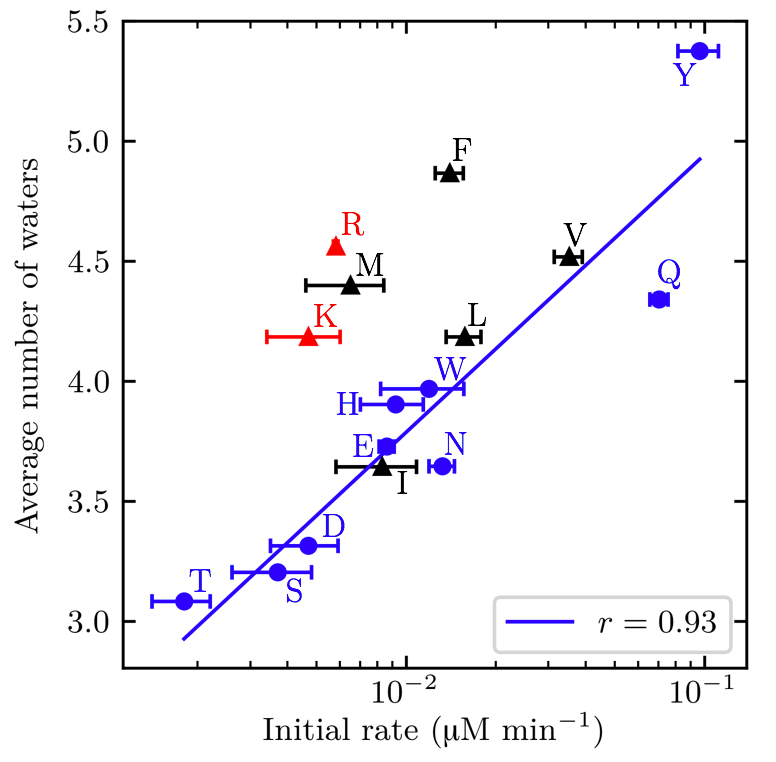
\includegraphics[width=\single]{figures-ras/Figure6.png}
    \caption{
        Boltzmann-weighted average number of waters in the active site per frame against the measured intrinsic rate. 
        To be considered in the active site, each water needed to be within 5 \si{\angstrom} of the Q61X side chain and within 5 \si{\angstrom} of the terminal phosphate oxygen of GTP (atom name O1G). 
        Blue: all polar or negatively charged side chains. 
        All other points are marked as triangles and are excluded from the fit. 
        Red: positively charged side chains. 
        Black: nonpolar side chains.
    }
    \label{fig:ras-scount}
\end{figure}

The positively charged residues (R and K) and the nonpolar residues (M, F, V, L, and I) are not included in the linear regression fit. 
Interestingly, it appears that the three branched nonpolar residues I, L, and V do still fit this same trend (including these residues in the fit does not change the correlation). 
However, without a concrete reason to include I, L, and V and exclude M and F, we have decided to omit all nonpolar residues from the trend. 
Indeed, if we consider the hydration potential of each residue as reported by Wolfenden et al.\cite{Wolfenden1981}, which quantifies the free energy of the transfer of the side chain from the vapor phase to buffered water, this distinction becomes even more interesting. 
When calculated in a vacuum, M and F are the only hydrophobic residues for which the transfer from the vapor phase to the solution phase occurs spontaneously, with negative hydration potentials (-1.48 and -0.76 kcal mol$^{-1}$, respectively, at pH 7), while, under the same conditions, the other hydrophobic residues I, L, and V had positive hydration potentials (2.15, 2.28, and 1.99 kcal mol$^{-1}$, respectively, at pH 7). 
This suggests that these two outliers have higher affinities for water and are changing the organization of water in the active site in some manner that is different from the other nonpolar residues. 
It is interesting that the positively charged and nonpolar residues had nonzero intrinsic hydrolysis rates, despite being unable to stabilize the transient hydronium ion. 
Without more information, it is impossible to determine if the rates are merely shifted from the correlation in Figure \ref{fig:ras-scount}, or if these mutants hydrolyzed GTP via an alternative mechanism that does not rely on the stabilization of a hydronium ion in the transition state.

Nevertheless, these results strongly support a multiwater intrinsic hydrolysis mechanism, such as the one shown in Figure \ref{fig:ras-mech}A, in which Q61 electrostatically stabilizes a hydronium ion in the transition state caused by the nucleophilic attack of a basic water molecule. 
In the case of the mechanism proposed by Buhrman et al., the hydronium ion is thought to be located between Q61, the bridging oxygen to the $\gamma$-phosphate, and a terminal oxygen on the $\gamma$-phosphate. 
This location was originally proposed based on observations from a crystal structure, which, by necessity, were obtained with the nonhydrolyzable GTP analogue 5'-guanylylimidodiphosphate (GppNHp) in the binding site. 
It is generally thought that the conversion of the bridging oxygen to a nitrogen between the second and third phosphate is a fairly conservative change, and it has allowed for the study of GTPases in the ON state. 
In the case of the VSE measurements by Stafford et al., which also relied on GppNHp, there should be very little difference in the results between GTP-bound Ras and GppNHp-bound Ras because the only observable perturbation at this distance should be electrostatic. 
However, the effect on the hydrogen bonding network caused by the switch of an oxygen to a nitrogen in the phosphate region may not be negligible. 
Indeed, in every one of our simulations of Q61X constructs with GTP, the bridging oxygen accepts a hydrogen bond from the amide backbone of G12. 
The interaction distances and number of hydrogen bonds per frame between these two groups are shown in Table \ref{tbl:ras-g12}. 
However, this interaction is not present in the crystal structure of Buhrman et al. 
The replacement of GTP with GppNHp in the crystallization replaces a hydrogen bond accepting oxygen (the bridging oxygen) with a hydrogen bond donating nitrogen, which could push G12 farther from the $\gamma$-phosphate, providing room for a water to be observed in between G12 and GppNHp. 
In our simulations, however, the hydrogen bond between G12 and GTP brings the protein backbone too close to allow for a water in this location. 
Therefore, while our data supports a multiwater mechanism in which Q61 electrostatically stabilizes a hydronium ion, which in turn stabilizes the transition state, we hypothesize that the hydronium ion must be elsewhere.

\begin{table}
    \caption[Interactions between GTP and residue G12 in Ras]{
        Interaction distances and probability of a hydrogen bond per frame between the amide nitrogen of G12 and the bridging oxygen (OS3) of GTP. 
        The standard deviations of the probabilities are omitted because they are of the same order of magnitude as the probabilities.
    }
    \begin{center}
    \begin{tabular}{ccc}
    \toprule
   \rowcolor{lgray}
    Ras construct & Interaction distance & Hydrogen bond probability\\
    \cmidrule(r){1-1}\cmidrule(rl){2-2}\cmidrule(l){3-3}
Q61D  & $2.86 \pm   0.12$ &   $0.54 $\\%\pm   0.50$  \\
Q61E  & $2.99 \pm   0.14$ &   $0.52 $\\%\pm   0.50$  \\
Q61F  & $2.87 \pm   0.12$ &   $0.50 $\\%\pm   0.50$  \\
Q61H  & $2.89 \pm   0.13$ &   $0.65 $\\%\pm   0.48$  \\
Q61I  & $2.90 \pm   0.14$ &   $0.71 $\\%\pm   0.45$  \\
Q61K  & $2.90 \pm   0.13$ &   $0.70 $\\%\pm   0.46$  \\
Q61L  & $2.88 \pm   0.13$ &   $0.47 $\\%\pm   0.50$  \\
Q61M  & $2.87 \pm   0.12$ &   $0.50 $\\%\pm   0.50$  \\
Q61N  & $2.86 \pm   0.12$ &   $0.52 $\\%\pm   0.50$  \\
Q61Q  & $2.85 \pm   0.11$ &   $0.53 $\\%\pm   0.50$  \\
Q61R  & $2.89 \pm   0.13$ &   $0.67 $\\%\pm   0.47$  \\
Q61S  & $2.88 \pm   0.12$ &   $0.49 $\\%\pm   0.50$  \\
Q61T  & $2.89 \pm   0.13$ &   $0.73 $\\%\pm   0.44$  \\
Q61V  & $2.89 \pm   0.14$ &   $0.43 $\\%\pm   0.50$  \\
Q61W  & $2.91 \pm   0.14$ &   $0.76 $\\%\pm   0.43$  \\
Q61Y  & $2.87 \pm   0.13$ &   $0.59 $\\%\pm   0.49$  \\

\bottomrule
\end{tabular}
    \end{center}
    \label{tbl:ras-g12}
\end{table}

Proposed mechanisms have also identified other residues in the region that could contribute to the intrinsic hydrolysis reaction, in particular Y32 identified in the mechanism proposed by Buhrman et al \cite{Buhrman2010}. 
Though mutant forms of residues other than G12, G13, and Q61 have not generally been identified as oncogenic, nor have they been reported as frequent mutations in tumors, Y32 is of interest to us because the Buhrman et al. mechanism suggests that it may be a secondary stabilizer of the transition state hydronium ion. 
However, our simulations were not set up to test specifically the mechanism proposed by Buhrman et al.; this is based on the crystal structure 3k8y where Y32 is oriented differently than our simulations based on 1lfd. 
Using simulations based on the crystal structure 3k8y and corresponding experiments, we are currently investigating the effect of mutations to Y32 on the intrinsic hydrolysis rate and will report these results in a later publication. 

Ultimately, the ability of each of these mutations to slow hydrolysis enough to convert Ras into an oncoprotein is based not only on its role in the intrinsic hydrolysis reaction but also on the likelihood that the DNA mutation causing these changes could occur. 
It is therefore not surprising that the oncogenic mutants of RasQ61X are also statistically the most likely to occur because they require the mutation of only a single nucleotide. 
The E, K, L, and R codons are only a single base switch away from the WT; the work described here demonstrates that any one of those changes results in a drastic suppression of intrinsic hydrolysis, leading to oncogenic effects which have been cataloged elsewhere \cite{Prior2012, Hobbs2016}. 
It has been suggested by Cox et al. that therapeutic strategies targeting the intrinsic hydrolysis mechanism of Ras may need to be mutation-specific\cite{Cox2014} and therefore require knowledge of the differences in the electrostatic contributions of these side chains. 
Our data set can be used to validate new computational models and inform future drug design efforts towards targeting the oncogenic forms of H-Ras. 

%%%%%%%%%%%%%%%%%%%%%%%%%%%%%%%%%%%%%%%%%%%%%%%%%%%%%%%%%%%%%%%%
%%%%%%%%%%%%%%%%%%%%%%%%%%%%%%%%%%%%%%%%%%%%%%%%%%%%%%%%%%%%%%%%
\section{Conclusions}\label{ras-conclusion}
%%%%%%%%%%%%%%%%%%%%%%%%%%%%%%%%%%%%%%%%%%%%%%%%%%%%%%%%%%%%%%%%
%%%%%%%%%%%%%%%%%%%%%%%%%%%%%%%%%%%%%%%%%%%%%%%%%%%%%%%%%%%%%%%%

We measured initial rates of intrinsic hydrolysis of GTP by WT Ras and 17 mutants of Q61. 
We compared the measured rates to previous measurements of nitrile probe frequency for each construct and found that polar and negatively charged residues, which are capable of stabilizing a hydronium ion, have initial rates that were normally distributed around a central nitrile frequency of $\sim$2163 \si{\wn}. 
Recently, using hybrid QM/MM simulations, Tichauer et al. arrived at a similar conclusion that also supports a multiwater mechanism for a closely related protein, N-Ras, by demonstrating that mutations at position 61 alter the distribution of waters in the active site \cite{Tichauer2018}. 
Similarly, we compared the initial rates to the average number of waters in the binding site calculated from MD simulations and showed that the number of waters in the binding site was strongly correlated with the initial rate for residues that can stabilize a hydronium ion. 
These observations support a multiwater mechanism of intrinsic hydrolysis, such as that of Buhrman et al. 
We further postulated that the proposed location of the transition state hydronium ion cannot be located at the bridging oxygen based on the observation of a hydrogen bond between G12 and GTP that was not present in the crystal structures that used the nonhydrolyzable GTP analogue, GppNHp. 
Together, these results form a data set that will be useful for validating computational models and potential future therapeutic strategies.



%%%%%%%%%%%%%%%%%%%%%%%%%%%%%%%%%%%%%%%%%%%%%%%%%%%%%%%%%%%%%%%%%%%%%%
% Appendix/Appendices                                                %
%%%%%%%%%%%%%%%%%%%%%%%%%%%%%%%%%%%%%%%%%%%%%%%%%%%%%%%%%%%%%%%%%%%%%%
%
% If you have only one appendix, use the command \appendix instead
% of \appendices.
%
%\appendices
%\index{Appendices@\emph{Appendices}}%
%
%\include{chapter-appendix1}
%
%\include{chapter-appendix2}
%
%\include{chapter-appendix3}


%%%%%%%%%%%%%%%%%%%%%%%%%%%%%%%%%%%%%%%%%%%%%%%%%%%%%%%%%%%%%%%%%%%%%%
% Generate the bibliography.					     %
%%%%%%%%%%%%%%%%%%%%%%%%%%%%%%%%%%%%%%%%%%%%%%%%%%%%%%%%%%%%%%%%%%%%%%
%								     %
% NOTE: For master's theses and reports, NOTHING is permitted to     %
%	come between the bibliography and the vita. The command      %
%	to generate the index (if used) MUST be moved to before      %
%	this section.						     %
%								     %
%\chapter{References}

%%Change Bibliography -> References
\renewcommand{\bibname}{References}
\addcontentsline{toc}{chapter}{References}
\bibliographystyle{achemso}
\bibliography{/Users/jfirst/Documents/Mendeley/Bibtex/library.bib,\jobname-control}
\index{References@\emph{References}}%			     %
%%%%%%%%%%%%%%%%%%%%%%%%%%%%%%%%%%%%%%%%%%%%%%%%%%%%%%%%%%%%%%%%%%%%%%


%%%%%%%%%%%%%%%%%%%%%%%%%%%%%%%%%%%%%%%%%%%%%%%%%%%%%%%%%%%%%%%%%%%%%%
% Generate the index.						     %
%%%%%%%%%%%%%%%%%%%%%%%%%%%%%%%%%%%%%%%%%%%%%%%%%%%%%%%%%%%%%%%%%%%%%%
%								     %
% NOTE: For master's theses and reports, NOTHING is permitted to     %
%	come between the bibliography and the vita. This section     %
%	to generate the index (if used) MUST be moved to before      %
%	the bibliography section.				     %
%								     %
%\printindex%    % Include the index here. Comment out this line      %
%		% with a percent sign if you do not want an index.   %
%%%%%%%%%%%%%%%%%%%%%%%%%%%%%%%%%%%%%%%%%%%%%%%%%%%%%%%%%%%%%%%%%%%%%%


%%%%%%%%%%%%%%%%%%%%%%%%%%%%%%%%%%%%%%%%%%%%%%%%%%%%%%%%%%%%%%%%%%%%%%
% Vita page.							     %
%%%%%%%%%%%%%%%%%%%%%%%%%%%%%%%%%%%%%%%%%%%%%%%%%%%%%%%%%%%%%%%%%%%%%%

%\begin{vita}
%Jeremy Todd First
%Is a vita even a real thing? If so, the text goes here and is a quick
%biography. Who would want to read about you? 
%\end{vita}

\end{document}
